%%%%%%%%%%%%%%%%%%%%%%%%%%%%%%%%%%%%%%%%%%%%%%%%%%%%%%%%%%%%%%%%%%%%%%%%%%%%%
%%%%%%                                                                  %%%%% 
%%%%%%          Maqueta de memòria TFC/PFC de l'EETAC                   %%%%% 
%%%%%%                                                                  %%%%% 
%%%%%%%%%%%%%%%%%%%%%%%%%%%%%%%%%%%%%%%%%%%%%%%%%%%%%%%%%%%%%%%%%%%%%%%%%%%%%
%%%%%%%%%%%%%%%%%%%%%%%%%%%%%%%%%%%%%%%%%%%%%%%%%%%%%%%%%%%%%%%%%%%%%%%%%%%%%
%%                                                                         %%
%%          Autor: Xavier Prats i Menéndez (xavier.prats@upc.edu)          %% 
%%                  Technical University of Catalonia (UPC)                %%
%%                                                                         %%
%%%%%%%%%%%%%%%%%%%%%%%%%%%%%%%%%%%%%%%%%%%%%%%%%%%%%%%%%%%%%%%%%%%%%%%%%%%%%
%%      This work is licensed under the Creative Commons  Attribution-     %%
%%   -Noncommercial-Share Alike 3.0 Spain License. To view a copy of this  %% 
%%    license, visit http://creativecommons.org/licenses/by-nc-sa/3.0/es/  %%
%%    or send a letter to Creative Commons, 171 Second Street, Suite 300,  %%
%%                  San Francisco,California, 94105, USA.                  %%
%%%%%%%%%%%%%%%%%%%%%%%%%%%%%%%%%%%%%%%%%%%%%%%%%%%%%%%%%%%%%%%%%%%%%%%%%%%%%
%% Versió 2.1 - Juliol 2012                                                %%
%%%%%%%%%%%%%%%%%%%%%%%%%%%%%%%%%%%%%%%%%%%%%%%%%%%%%%%%%%%%%%%%%%%%%%%%%%%%%

%%% NOTA: els seguents packages son necessaris per utilitzar la
%%%       plantilla seguent:
%%%       ifthen,calc,helvet,pslatex,fancyhdr,nextpage,subfigure,tocloft,graphicx,url

%%% NOTA: Es possible que algunes distribuicions Linux o Windows.
%%%       no portin aquests paquets instal·lats per defecte.
%%%       En aquest cas els haureu d'instal·lar manualment.


%%%%%%%%%%%%%%%%%%%%%%%%%%%%%%%%%%%%%%%%%%%%%%%%%%%%%%%%%%%%%%%%%%%%%%%%%%%%%
% 1- INICIALITZACIÓ
%%%%%%%%%%%%%%%%%%%%%%%%%%%%%%%%%%%%%%%%%%%%%%%%%%%%%%%%%%%%%%%%%%%%%%%%%%%%%

\documentclass[spanish,final]{setup/eetac_tfc_pfc}
%% * OPCIONS A CONFIGURAR al \documentclass
%%    - Estat del document: final o draft
%%      NOTA: Draft no inserta les figures i marca només l'espai que
%%      ocupen. També s'indica quan el text sobrepassa els marges.
%%      Draft és molt útil per compilar ràpid el document si no és important
%%      en aquell moment visualitzar les figures.
%%    - Idioma PRINCIPAL del document: catalan, spanish, english, french...

\usepackage[english,spanish]{babel}
%%  * INCLOURE TOTS ELS IDIOMES QUE S'USARAN EN EL DOCUMENT
%%    NOTA: per canviar d'idioma al mig del document usar:
%%          \selectlanguage{nom_idioma}
%%%%%%%%%%%%%%%%%%%%%%%%%%%%%%%%%%%%%%%%%%%%%%%%%%%%%%%%%%%%%%%%%%%%%%%%%%%%%

%%%%%%%%%%%%%%%%%%%%%%%%%%%%%%%%%%%%%%%%%%%%%%%%%%%%%%%%%%%%%%%%%%%%%%%%%%%%%
% 2- CÀRREGA DE PAQUETS ADICIONALS (OPCIONALS)
%%%%%%%%%%%%%%%%%%%%%%%%%%%%%%%%%%%%%%%%%%%%%%%%%%%%%%%%%%%%%%%%%%%%%%%%%%%%%

%%% NOTA: Es possible que algunes distribuicions Linux o Windows.
%%%       no portin aquests paquets instal·lats per defecte.
%%%       En aquest cas els haureu d'instal·lar manualment.

%% El paquet inputenc és extramadament útil. 
%% Permet escriure els accents directament amb l'editor de texte
%% sense haver de fer coses com per exemple: introducci\'o
%% Heu d'especificar la codificació de caracters que utilitzeu pel
%% vostre fitxer (en aquest exemple utf8)
\usepackage[utf8]{inputenc}

%% Símbols matemàtics de la American Mathematical Society
\usepackage{amssymb,amsmath, amsfonts}  

%% El paquet array proporciona eines molt útils a l'hora de fer 
%% equacions amb matrius
\usepackage{array}             

%% Paquet que permet fer taules fusionant cel·les de files consecutives
\usepackage{multirow}          

%% Paquet molt útil en cas de tenir taules molt llargues que 
%   ocupin vàries pàgines
\usepackage{longtable}          

%% Permet canviar els colors del document
%\usepackage{color,colortbl}

%% Paquet molt útil que permet activar links en el PDF final.
%% * NO OBLIDAR DE CONFIGURAR els quatre primer camps!
\usepackage[
  pdfauthor={Rodrigo Sampedro Casis},            % Configurar adientment
  %pdftitle={Treball Fi de Carrera - autor}, % Configurar adientment
  %pdfsubject={Titol del TFC aqui},          % Configurar adientment
  % Modificació respecte a la versió 2.1 - Iván Padilla Montero - Juliol 2014
  pdftitle={Treball Fi de Grau - autor}, % Configurar adientment
  pdfsubject={Desarrollo de una Oficina de Ingeniería Remota: Análisis y Implementación de una Solución en el Contexto del Teletrabajo},          % Configurar adientment  
  pdfkeywords={keyword1, keyword2, ...},    % Configurar adientment
  pdfcreator={EETAC-UPC}, 
  pdfproducer={LaTeX, dvipdf},
  pdfdisplaydoctitle=true, plainpages=false, linktocpage=true,         
  colorlinks=true, linkcolor=blue,citecolor=blue,urlcolor=blue,
  hyperfootnotes=false, pagebackref=true, pdfpagelabels=true,
  pdfpagemode=UseOutlines,
]{hyperref} 

%% NOTA IMPORTANT!:
%% Per tal que hyperef funcioni correctament amb els capitols o seccions no
%% numerats (\chapter*{}), com per exemple introducció, conclusions i bibliografia
%% cal posar les dues comandes seguents ABANS del \chapter*{} en questió
%\cleardoublepage
%\phantomsection

%% Permet trencar links URL. 
%% Atenció! afegir aquest paquet DESPRES del hyperref!!
\usepackage{breakurl} 

%% Permet arranjar matricialment multiples figures
%% NOTA: afegir aquest paquet DESPRES del hyperref!!
%%       Si no es desitja utilitzar aquest paquet, comentar la linia seguent
%%       i anar TAMBE al fitxer de classe (eetac_tfc_pfc.cls) per substituir: 
%%       \RequirePackage[subfigure]{tocloft}  per  \RequirePackage{tocloft}
\usepackage{subfigmat}         


% definicion de bloques de codigo
\usepackage{listings}
\usepackage{xcolor}

\definecolor{codegreen}{rgb}{0,0.6,0}
\definecolor{codegray}{rgb}{0.5,0.5,0.5}
\definecolor{codepurple}{rgb}{0.58,0,0.82}
\definecolor{backcolour}{rgb}{0.95,0.95,0.92}


\lstdefinestyle{yaml}{
     basicstyle=\color{blue}\footnotesize,
     rulecolor=\color{black},
     string=[s]{'}{'},
     stringstyle=\color{blue},
     comment=[l]{:},
     commentstyle=\color{black},
     morecomment=[l]{-}
 }

\lstdefinestyle{mystyle}{
    backgroundcolor=\color{backcolour},   
    commentstyle=\color{codegreen},
    keywordstyle=\color{magenta},
    numberstyle=\tiny\color{codegray},
    stringstyle=\color{codepurple},
    basicstyle=\ttfamily\footnotesize,
    breakatwhitespace=false,         
    breaklines=true,                 
    captionpos=b,                    
    keepspaces=true,                                   
    showspaces=false,                
    showstringspaces=false,
    showtabs=false,                  
    tabsize=2
}

\lstdefinestyle{customc}{
  belowcaptionskip=1\baselineskip,
  breaklines=true,
  frame=L,
  xleftmargin=\parindent,
  language=C,
  showstringspaces=false,
  basicstyle=\footnotesize\ttfamily,
  keywordstyle=\bfseries\color{green!40!black},
  commentstyle=\itshape\color{purple!40!black},
  identifierstyle=\color{blue},
  stringstyle=\color{orange},
}

\lstdefinestyle{yaml}{
     basicstyle=\color{blue}\footnotesize,
     rulecolor=\color{black},
     string=[s]{'}{'},
     stringstyle=\color{blue},
     comment=[l]{:},
     commentstyle=\color{black},
     morecomment=[l]{-}
 }


\lstset{style=mystyle}

\renewcommand\lstlistingname{Code}
\renewcommand\lstlistlistingname{Bloques de Código}
\newcommand{\tony}[1]{\textcolor[rgb]{0.0,0.0,1.0}{#1}}

%%%%%%%%%%%%%%%%%%%%%%%%%%%%%%%%%%%%%%%%%%%%%%%%%%%%%%%%%%%%%%%%%%%%%%%%%%%%%


%%%%%%%%%%%%%%%%%%%%%%%%%%%%%%%%%%%%%%%%%%%%%%%%%%%%%%%%%%%%%%%%%%%%%%%%%%%%%
% 3- DOCUMENT
%%%%%%%%%%%%%%%%%%%%%%%%%%%%%%%%%%%%%%%%%%%%%%%%%%%%%%%%%%%%%%%%%%%%%%%%%%%%%

%%% Configuració de les dades i variables boleanes rellevants del document:
%%%%%%%%%%%%%%%%%%%%%%%%%%%%%%%%%%%%%%%%%%%%%%%%%%%%%%%%%%%%%%%%%%%%%%%%%%%%%
%%%%%%                                                                  %%%%% 
%%%%%%       Fitxer de dades per la memoria TFC/PFC de l'EETAC          %%%%% 
%%%%%%                                                                  %%%%% 
%%%%%%%%%%%%%%%%%%%%%%%%%%%%%%%%%%%%%%%%%%%%%%%%%%%%%%%%%%%%%%%%%%%%%%%%%%%%%
%%%%%%%%%%%%%%%%%%%%%%%%%%%%%%%%%%%%%%%%%%%%%%%%%%%%%%%%%%%%%%%%%%%%%%%%%%%%%
%%                                                                         %%
%%          Autor: Xavier Prats i Menendez (xavier.prats@upc.edu)          %% 
%%                  Technical University of Catalonia (UPC)                %%
%%                                                                         %%
%%%%%%%%%%%%%%%%%%%%%%%%%%%%%%%%%%%%%%%%%%%%%%%%%%%%%%%%%%%%%%%%%%%%%%%%%%%%%
%%      This work is licensed under the Creative Commons  Attribution-     %%
%%   -Noncommercial-Share Alike 3.0 Spain License. To view a copy of this  %% 
%%    license, visit http://creativecommons.org/licenses/by-nc-sa/3.0/es/  %%
%%    or send a letter to Creative Commons, 171 Second Street, Suite 300,  %%
%%                  San Francisco,California, 94105, USA.                  %%
%%%%%%%%%%%%%%%%%%%%%%%%%%%%%%%%%%%%%%%%%%%%%%%%%%%%%%%%%%%%%%%%%%%%%%%%%%%%%
%% Versio 2.1 - Juliol 2012                                                %%
%%%%%%%%%%%%%%%%%%%%%%%%%%%%%%%%%%%%%%%%%%%%%%%%%%%%%%%%%%%%%%%%%%%%%%%%%%%%%

%%%%%%%%%%%%%%%%%%%%%%%%%%%%%%%%%%%%%%%%%%%%%%%%%%%%%%%%%%%%%%%%%%%%%%%%%%%%%%%
%%  VARIABLES A CONFIGURAR                                                  %%%
%%%%%%%%%%%%%%%%%%%%%%%%%%%%%%%%%%%%%%%%%%%%%%%%%%%%%%%%%%%%%%%%%%%%%%%%%%%%%%%

%% - Projecte o Treball de Fi de Carrera?
%%      PFC = true   -> Projecte de Fi de Carrera
%%      PFC = false  -> Treball  de Fi de Carrera
\setboolean{PFC}{false}

%% - Escollir la titulació
%\titulacio{Enginyeria Tècnica Aeronàutica, especialitat Aeronavegació}
%\titulacio{Enginyeria T\`ecnica de Telecomunicaci\'o, especialitat Sistemes de Telecomunicaci\'o}
%\titulacio{Enginyeria T\`ecnica de Telecomunicaci\'o, especialitat Telem\`atica}
%\titulacio{Enginyeria de Telecomunicaci\'o (segon cicle)}
% Modificació respecte a la versió 2.1 - Iván Padilla Montero - Juliol 2014
%\titulacio{Grau en Enginyeria d'Aeronavegaci\'o}
%\titulacio{Grau en Enginyeria d'Aeroports}
\titulacio{Grado en Ingenieria Telematica}
%\titulacio{Grau en Enginyeria de Sistemes de Telecomunicació}


%% - Configurar els idiomes del document
%% Si l'idioma PRINCIPAL del document es l'angles, posar aquesta variable a true
\setboolean{Leng}{false}

%% Escollir entre catala i castella (idioma principial, o nomes pel resum en cas que l'idioma principal sigui anglès)
%%  catala = true   -> idioma principal (o només resum) en Català
%%  catala = false  -> idioma principal (o només resum) en Castella
\setboolean{Lcat}{false}

%% Titol del document en l'idioma principal del document 
\titol{Desarrollo de una Oficina de Ingeniería Remota: Análisis y Implementación de una Solución en el Contexto del Teletrabajo}

%% Titol del document en anglès (Per l'apartat overview)
\titolE{Development of a Remote Engineering Office: Analysis and Implementation of a Solution in the Context of Home Office}

%% Titol del document en catala/castella (Per l'apartat resum)
\titolC{Desarrollo de una Oficina de Ingeniería Remota: Análisis y Implementación de una Solución en el Contexto del Teletrabajo}


%% - Nombre d'autors del TFC/PFC?
%%      UNautor = true   Un sol autor
%%      UNautor = false  Més d'un autor
\setboolean{UNautor}{true}

%% - Nom del(s) Autor(s) del document
%% NOTA: En cas de mes d'un autor cal posar la comana \and entre els
%%        noms dels autors
\autor{Rodrigo Sampedro Casis}

%% - Nombre de directors del TFC/PFC. Tipicament 1 o 2
%%      UNdirector = true   Un sol director
%%      UNdirector = false  Dos directors
\setboolean{UNdirector}{true}

%% - Nom del Director del TFC/PFC
\director{Antonio Marzoa Domínguez}

%% - Nom del segon director en cas de tenir-lo:
\segonDirector{Nom2 Cognoms2}


%% - Es vol incloure una dedicatoria?
%%      dedicatoria = true   -> S'afegeix una pagina amb \textDedicatoria
%%      dedicatoria = true   -> No s'afegeix dedicatoria
%% NOTA: no confondre dedicatòria amb agraïments. Una dedicatoria sol ser
%%       un missatge curt d'una o dues frases màxim a la persona, o persones
%%       a les quals es dedica el treball. 
%%       Els agraïments poden ser extensos i l'autor pot agraïr a diverses
%%       persones coses diferents en funció de l'ajuda rebuda, per exemple. 
%%       Si es volen incloure agraïments, fer-ho al fitxer de la 
%%       memòria creant una secció nova amb  \chapter*{Agraïments}
\setboolean{dedicatoria}{true}
\textDedicatoria{a Chloe promotora de la idea}

%% - Es vol incloure una pagina d'index de figures?
\setboolean{paginaLOF}{true}  % List of Figures

%% - Es vol incloure una pagina d'index de taules?
\setboolean{paginaLOT}{true}  % List of Tables 

%% - El projecte ha estat supervisat per alguna persona externa? 
%%   (NOMES en cas de practiques en empresa)
%%      supervisor = true    -> Hi ha un supervisor
%%      supervisor = false   -> No hi ha un supervisor
\setboolean{supervisor}{false}

%% NOMES en el cas de practiques en empresa (supervisor=true) s'han de 
%% configurar les variables seguents: 

%% Supervisor del TFC/PFC 
\supervisor{Nom del Supervisor}

%% - Es vol incloure el logotip de l'empresa?
%%   En el cas que el TFC/PFC s'hagi fet en règim d'intercanvi amb una
%%   empresa, es pot afegir el seu logotip a la cantonada superior
%%   dreta de la portada. En aquest cas:
%%   - posar logo=true
%%   - posar el path de la imatge i l'alçada del logo a \mylogo
\setboolean{logo}{false}
\mylogo{./setup/EETAC-positiu-negre}{1.5cm}
  

%%% Configuració de MACROS o ENTORNS (opcionals) definides per l'usuari:
%%%%%%%%%%%%%%%%%%%%%%%%%%%%%%%%%%%%%%%%%%%%%%%%%%%%%%%%%%%%%%%%%%%%%%%%%%%%%
%%%%%%                                                                  %%%%% 
%%%%%%    Fitxer de macros d'usuari per la memoria TFC/PFC de l'EETAC   %%%%% 
%%%%%%                                                                  %%%%% 
%%%%%%%%%%%%%%%%%%%%%%%%%%%%%%%%%%%%%%%%%%%%%%%%%%%%%%%%%%%%%%%%%%%%%%%%%%%%%
%%%%%%%%%%%%%%%%%%%%%%%%%%%%%%%%%%%%%%%%%%%%%%%%%%%%%%%%%%%%%%%%%%%%%%%%%%%%%
%%                                                                         %%
%%         Author: Xavier Prats i Menendez (xavier.prats@upc.edu)          %% 
%%                  Technical University of Catalonia (UPC)                %%
%%                                                                         %%
%%%%%%%%%%%%%%%%%%%%%%%%%%%%%%%%%%%%%%%%%%%%%%%%%%%%%%%%%%%%%%%%%%%%%%%%%%%%%
%%      This work is licensed under the Creative Commons  Attribution-     %%
%%   -Noncommercial-Share Alike 3.0 Spain License. To view a copy of this  %% 
%%    license, visit http://creativecommons.org/licenses/by-nc-sa/3.0/es/  %%
%%    or send a letter to Creative Commons, 171 Second Street, Suite 300,  %%
%%                  San Francisco,California, 94105, USA.                  %%
%%%%%%%%%%%%%%%%%%%%%%%%%%%%%%%%%%%%%%%%%%%%%%%%%%%%%%%%%%%%%%%%%%%%%%%%%%%%%
%% Versio 1.5 - Juliol 2010                                                %%
%%%%%%%%%%%%%%%%%%%%%%%%%%%%%%%%%%%%%%%%%%%%%%%%%%%%%%%%%%%%%%%%%%%%%%%%%%%%%


%%% Xevi's macros for vectors and matrices:

%\newcommand{\ve}[1]{\mbox{\boldmath$#1$}}          
\newcommand{\ve}[1]{\vec{#1}}  
\newcommand{\ma}[1]{\mbox{\boldmath$\mathcal{#1}$}}

%%% Xevi's macros for brackets:
\newcommand{\lp}{\left(}
\newcommand{\lc}{\left[}
\newcommand{\lcl}{\left\{}
\newcommand{\rp}{\right)}
\newcommand{\rc}{\right]}
\newcommand{\rcl}{\right\}}

%%% Xevi's new environment for HIPOTESIS
\newcounter{num_hyp}
\newenvironment{hyp}[2]{
        \refstepcounter{num_hyp}
        \vspace*{2.5ex}
        {\noindent \bf\sffamily HYPOTHESIS #1 : #2} \\
        \sl
}
        {\vspace{1ex}
}

\newcommand{\SUMhyp}[2]{
 {\sffamily HYPOTHESIS #1 : #2} 
}
  

%%% Configuració manual de les regles d'hyphenation:
%%%%%%%%%%%%%%%%%%%%%%%%%%%%%%%%%%%%%%%%%%%%%%%%%%%%%%%%%%%%%%%%%%%%%%%%%%%%%
%%%%%%                                                                  %%%%% 
%%%%%%    Fitxer de hyphenation per la memoria TFC/PFC de l'EETAC       %%%%% 
%%%%%%                                                                  %%%%% 
%%%%%%%%%%%%%%%%%%%%%%%%%%%%%%%%%%%%%%%%%%%%%%%%%%%%%%%%%%%%%%%%%%%%%%%%%%%%%
%%%%%%%%%%%%%%%%%%%%%%%%%%%%%%%%%%%%%%%%%%%%%%%%%%%%%%%%%%%%%%%%%%%%%%%%%%%%%
%%                                                                         %%
%%         Author: Xavier Prats i Menendez (xavier.prats@upc.edu)          %% 
%%                  Technical University of Catalonia (UPC)                %%
%%                                                                         %%
%%%%%%%%%%%%%%%%%%%%%%%%%%%%%%%%%%%%%%%%%%%%%%%%%%%%%%%%%%%%%%%%%%%%%%%%%%%%%
%%      This work is licensed under the Creative Commons  Attribution-     %%
%%   -Noncommercial-Share Alike 3.0 Spain License. To view a copy of this  %% 
%%    license, visit http://creativecommons.org/licenses/by-nc-sa/3.0/es/  %%
%%    or send a letter to Creative Commons, 171 Second Street, Suite 300,  %%
%%                  San Francisco,California, 94105, USA.                  %%
%%%%%%%%%%%%%%%%%%%%%%%%%%%%%%%%%%%%%%%%%%%%%%%%%%%%%%%%%%%%%%%%%%%%%%%%%%%%%
%% Versio 1.5 - Juliol 2010                                                %%
%%%%%%%%%%%%%%%%%%%%%%%%%%%%%%%%%%%%%%%%%%%%%%%%%%%%%%%%%%%%%%%%%%%%%%%%%%%%%

\hyphenation{Cas-tell-de-fels}
\hyphenation{EETAC}
  

\begin{document}

%% Seleccionar l'idioma principal del document:
\selectlanguage{spanish}

\beforepreface  

%% RESUM i OVERVIEW
%%%%%%%%%%%%%%%%%%%%%%%%%%%%%%%%%%%%%%%%%%%%%%%%%%%%%%%%%%%%%%%%%%%%%%%%%%%%%
% NOTA: les longituds passades com a parametres d'entrada  s'han
%        d'ajustar manualment fins que el requadre del resum/overview
%        ocupi tota la pàgina. 

%%% Resum en català (o castellà)
\selectlanguage{spanish}   
\begin{resum}{10cm}
Actualmente el mundo tecnológico sufre una expansión sin precedentes debido a la cuarta revolución industrial\cite{c_revolucion_4_0} y el acceso o actualización de las pequeñas y medianas empresas a las tecnologías de la información\cite{c_pyme_digital}. Esto ha supuesto la llegada de una amplia oferta de empleos de escasa inversión material, alta capacitación curricular y la posibilidad de des localización de los empleados, favoreciendo el crecimiento de lo que se ha venido a conocer como “la ingeniería en remoto”\cite{c_remote_work_stat_uk} \cite{c_remote_work_stat_talent}. Los empleados que han entrado en este nuevo  ambiente de trabajo, tienen herramientas similares debido a su condición de “remoto” mayoritario, independientemente de si pertenecen a una gran empresa o una startup, sean freelances o subcontratados por consultoras externas.\newline
\newline
Paralelamente, tras la pandemia de COV-19\cite{c_covid_remote}, se ha evidenciado la necesidad y facilidad del trabajo en remoto así como la conciliación del home office. Sin embargo, ha creado la falacia del ingeniero con un ordenador, capaz de trabajar desde casa con compañeros que no se conocen físicamente, así como la vuelta irremediable a la oficina por pérdida de productividad en muchas empresas\cite{c_back_office}.\newline
\newline
Este TFG  analiza, evalúa e implementa una solución a la creación de una oficina de desarrollo de ingeniería en remoto, explotada y utilizada por el propio autor del mismo, detallando los problemas encontrados y las soluciones halladas e implementadas durante la construcción de esta. \newline
\newline
En los anexos se resume el estado de arte de los principales puntos de interés, especialmente en el ámbito tecnológico, así como se presenta una posible guía para la puesta en marcha de una startup tecnológica a partir del trabajo realizado, y desde un punto de vista técnico, puesto que los requisitos son tanto aplicables para un trabajador en remoto, como para un trabajador por cuenta ajena, o bien aplicable al desarrollo inicial de una empresa con pocos trabajadores.\newline
\newline
 El objetivo principal es obtener un set mínimo de recursos que permitan de una manera genérica, sin un coste excesivo, permitir un correcto desarrollo de la actividad, sorteando problemas y facilitando la creación de herramientas de trabajo colaborativo.\newline
\newline
Asimismo se ha utilizado esta plantilla como base de proyectos personales y como implementación activa en varias empresas pyme de familiares y amigos del propio autor.

\end{resum}

%%% Resum en anglès
\selectlanguage{english}   
\begin{overview}{10cm}
At the moment, the technological world is undergoing an unprecedented expansion due to the fourth industrial revolution\cite{c_revolucion_4_0} and the access or update of small and medium-sized enterprises to information technologies\cite{c_pyme_digital}. This has led to the emergence of a wide range of jobs with low material investment, the requirement of high curriculum qualification, and the possibility of employee delocalization, promoting the growth of what has come to be known as "remote engineering"\cite{c_remote_work_stat_uk} \cite{c_remote_work_stat_talent}. Employees who have entered this new work environment use similar tools due to their predominantly "remote" condition, regardless of whether they belong to a large company or a startup, or being freelancers, or being subcontracted by external consulting firms.\newline
\newline
In parallel, the COVID-19 pandemic\cite{c_covid_remote}, the need and ease of remote work, as well as the balance of home office, have become evident. However, it has created the fallacy of the engineer with a computer, capable of working from home with colleagues they have never met physically, as well as the inevitable return to the office due to a loss of productivity in many companies\cite{c_back_office}.\newline
\newline
This Bachelor's Degree analyzes, evaluates, and implements a solution for creating a remote engineering development office, used by the author on his own, detailing and explaining the problems and solutions undertaken during its construction.\newline
\newline
In the appendices, the state of the art of the main points of interest regarding the project is summarized, especially in the technological field, and a possible guide for launching a technology startup from a technical perspective is presented since the requirements are applicable to both remote and in-house workers, or even to the initial development of a company with few employees.\newline
\newline
The main goal is to obtain a minimal set of resources that, in a fairly generic manner and without excessive cost, enable the proper development of activities, overcoming challenges, and facilitating the creation of collaborative work tools.\newline
\newline
Furthermore, this template has been used as the basis for personal projects and actively implemented in several family and friend-owned SMEs.

\end{overview}

% Tornar a l'idioma principal del document
\selectlanguage{spanish}  

%NOTA: En cas d'utilitzar l'espanyol com a idioma principal del document, el
%      latex anomena les taules com a 'Cuadros'. Si es desitja canviar aquesta
%      nomenclatura i utilitzar la paraula 'Tabla' descomentar les línies següents:
\def\listtablename{Índice de tablas}
\def\tablename{Tabla}%


% Amb aqueta comanda indiquem que ja s'han inclòs tots els apartats del prefaci del 
% projecte o podem començar a incloure els capitols de la memòria
\afterpreface

\clearpage





%%%%%%%%%%%%%%%%%%%%%%%%%%%%%%%%%%%%%%%%%%%%%%%%%%%%%%%%%%%%%%%%%%%%%%%%%%
%%%%%% INCLOURE A PARTIR D'AQUÍ TOTS ELS CAPÍTOLS DE LA MEMORIA   %%%%%%%%
%%%%%%%%%%%%%%%%%%%%%%%%%%%%%%%%%%%%%%%%%%%%%%%%%%%%%%%%%%%%%%%%%%%%%%%%%%

% NOTA: recordar que la introducció i les conclusions són capítols NO
%       enumerats, per tant s'ha d'usar \chapter*

% NOTA: és aconsellable incloure els capítols de la memòria en fitxers 
%       separats utlitzant la comanda \input  Per exemple:
%       \input{capitol1}  
%       que farà que s'inclogui el fitxer capitol1.tex

% NOTA: Si es vol incloure agraïments i/o glosari, fer-ho utilitzant 
% \chapter*{} i incloure'ls abans la introducció

\cleardoublepage
\phantomsection
\chapter*{Introducción}
Este TFG esta centrado en el concepto de teletrabajo y mas específicamente en los requisitos, herramientas y conceptos que se aplican en un trabajo remoto profesional. El caso de estudio se centra en la solución realizada a un problema logístico y familiar, para habilitar un espacio adecuado para el teletrabajo y las herramientas necesarias tanto desde el punto de vista del trabajador como desde la infraestructura en la nube de una empresa.

\section{Objetivos}
Los objetivos de este TFG son:
\begin{itemize}
    \item Planificar y solventar la necesidad de un espacio de teletrabajo (para este autor) y facilitar el home-office o flexwork, para la pareja del autor, debido a la incorporación de un nuevo miembro a la familia (Chloe).  
    
    \item Investigar, recopilar y resumir un estado del arte tanto infraestructura (física) como herramientas e infraestructura de software (virtuales).
    
    \item Definir los requisitos y un ejemplo de implementación de una oficina física, para la realización del teletrabajo de este autor. Implementarlo y evaluar los resultados o puntos de mejora y comparativas con oficinas / setups previos.
    
    \item Definir e implementar, una nube con los servicios mínimos para realizar teletrabajo, de especial interés para autónomos, pequeñas y medianas empresas o startups tecnológicas.
    
    \item Simplificar y automatizar el proceso, con el objetivo de poder usar el resultado practico de este TFG, como elemento genérico o producto fácilmente desplegable sin necesidad de conocimientos profundos.

\end{itemize}

\section{Requisitos}

La definición de trabajo en remoto, difiere según el porcentaje de jornada laboral realizada;  la ubicación desde dónde se realiza; la topología y forma de la empresa y el estatus jurídico del trabajador.  En el anexo \ref{S:anexo_A}, se desarrollan los diferentes tipos o escalas de teletrabajo, sin embargo la casi totalidad de desarrollo técnico de \textbf{este documento se centra en la modalidad de “home office” de un 60-100\%}, es decir, trabajar desde casa e ir 1-2 días por semana o en ocasiones específicas. Por consiguiente una parte importante de este documento se centra en los requisitos y caso practico de 'una oficina física de desarrollo tecnológico' para teletrabajar.

¿Qué entendemos como una oficina de desarrollo tecnológico? Todos aquellos trabajos que se involucran en el desarrollo (mantenimiento o creación)  de productos/servicios tecnológicos. Esto está intrínsecamente relacionado con software y una de las siguientes necesidades más demandadas por pymes (pequeña y mediana empresa):

\begin{itemize}
    \item Desarrollo de software: sin incluir los nuevos productos, existe una necesidad de digitalizar todo proceso en papel, manual o burocrático así como actualizar viejos software para su uso extendido en ‘la nube’; o el digital twin\cite{c_digital_twin} que permite representar elementos físicos en el mundo digital y realizar simulaciones. 

    \item Infraestructura en la nube:  permitir el acceso des-localizado, el escalado y la flexibilidad de gestión al tener recursos en una nube, tanto como servicio como el soporte asociado.
    
    \item Infraestructura tecnológica (redes \& hardware), acceso, actualización y puesta en marcha tanto de servidores, seguridad, sensores, oficinas o elementos para el teletrabajo.
    
    \item Análisis de datos: existe un nuevo mercado basado en la gran cantidad de datos y el minado y procesado de los mismos con fines optimizadores o como subproducto derivado.
    
    \item Electrónica, sensores, impresión 3D y prototipado: puede resumirse en llevar las nuevas tecnologías low cost al mercado tradicional, permitiendo un grado tecnológico en pequeñas empresas o explotaciones, anteriormente solo utilizado en grandes empresas.

    \item Ciberseguridad y temas legislativos: los nuevos riesgos y deberes implica que una actividad se digitalice.

\end{itemize}

¿Qué significa esto para los requisitos de nuestra oficina de desarrollo? Básicamente que un componente muy significativo obligatorio debe estar centrado en la infraestructura física del trabajador y la gestión o creación de una nube digital por parte de la empresa. 

Independientemente de que tipo de trabajador y donde sea el lugar de la actividad ¿Qué necesita un técnico para desarrollar un trabajo en remoto?

\begin{itemize}
    \item Un espacio físico, internet, luz, hardware, temperatura, control de horarios … que nombraremos requisitos físicos.
    
    \item Software y plataforma de comunicación directa, ya sean salas, teléfono, herramientas informáticas (correo,  videoconferencia, red social corporativa, página web), organizar/almacenar/monitorizar el trabajo realizado.

    \item Redes, Vpn, capas de seguridad de aislamientos, seguridad.
    
    \item Wiki, documentación, guías o código de buenas prácticas, que no solo faciliten la producción de los proyectos sino que eviten problemas estructurales y promuevan un mantenimiento ágil así como definen la dinámica de trabajo desde el punto de vista humano.
    
\end{itemize}

Durante los diferentes apartados de este documento, se irán desglosando los diferentes temáticas de interés iniciando desde un punto de vista genérico dando paso a un caso específico para finalmente exponer la implementación de “mi oficina” realizada por este autor, y la nube digital asociada. El documento principal introduce y desarrolla las utilidades y conceptos utilizadas así como los resultados obtenidos pero la gran parte del contexto, razonamientos y detalles o comparativas se predisponen en los anexos adjuntos o en algunos casos en documentos externos no adscritos a esta memoria.

Este TFG esta segmentado en 3 partes, capitulo \ref{S:tema_1}, anexos \ref{S:anexo_A} y \ref{S:anexo_B}, focalizados en la perspectiva del trabajador. Capitulo \ref{S:tema_2} y \ref{S:tema_3} y anexos \ref{S:anexo_C}, \ref{S:anexo_D}, \ref{S:anexo_E} focalizados en la infraestructura necesaria desde el punto de vista técnico-empresarial. Y capitulo \ref{S:tema_4} centrado en las dinámicas de trabajo en grupo, buenas practicas o metodología en desarrollo de software.

Finalmente en el anexo \ref{S:anexo_F} las conclusiones obtenidas en casos reales al implementar la base proporcionada por la 'oficina física y virtual', se evalúan y mencionan varios sub-proyecto personales así como la aplicación en varios negocios reales.

\chapter{Oficina física}\label{S:tema_1}
Este tema define los requisitos teóricos de la construcción de una oficina en remoto, contrastada con dos setups, uno mi habitación de estudio reconvertida en oficina durante la pandemia de 2020-21 véase \ref{S:setup_pandemia} y el diseño implementación y uso de “mi oficina-virtual” durante 2022-23. Los requisitos se catalogan en 7 categorías (véase anexo \ref{S:requisitos}), \textbf{mínimo, adecuado y óptimo} respecto a la calidad del requisito; y \textbf{básico, profesional, profesional pro y business} en relación a el coste.


\section{Requisitos}
En este apartado se define la base adecuada para una oficina en casa o también útil como base elemental de oficina para una startup tecnológica.

\subsection{Elementos físicos}
Entendemos como mínimo indispensable un pc o laptop para realizar la tarea, sin embargo esto es “la falacia estudiantil”. Realizar un trabajo profesional de manera continuada ( 8 horas), sin interrupciones y concentrado no debe llevarse a cabo en espacios públicos o familiares. Las malas condiciones posturales así como climatización o la inestabilidad de servicios claves como internet degradan la calidad final del trabajo\cite{c_postura} y contribuyen psicológicamente en una actitud negativa del trabajador\cite{c_postura_covid}.

 Está claro que un elemento implícito es el espacio de trabajo, una habitación, un cubículo, un coworking, su principal función es permitir instalar en el el setup informático quien es el verdadero centro de la oficina. Pero otros aspectos como tener una iluminación y ventilación adecuada, así como facilitar la organización de apuntes, herramientas o periféricos necesarios durante la jornada laboral son tan importantes como el propio setup.

Finalmente se ha definido espacialmente, el doble del tamaño de un cubículo de las bibliotecas de UPC como el espacio adecuado y una habitación dedicada como óptima. 

\subsection{Setup informático}
En el anexo \ref{S:setup_informatico} mencionan las principales corrientes en la selección y montaje de un setup. En mi opinión y como conclusión se recomienda encarecidamente un setup basado en laptop, aunque puede utilizarse un pc o mini pc. Es requisito indispensable un monitor extendido de 24’-27’, aunque se recomienda el uso de dos pantallas (\ref{S:pantallas}). El uso de periféricos tales como ratón/teclado, auriculares con micrófono, todos ellos conectados a través de un elemento centralizador de interconexión de pantallas, pc/laptop.

Respecto al hardware existe una evolución histórica\cite{c_guia_hardware}, cuellos de botella y estrategias a la hora de planificar la compra y mantenimiento de los diferentes componentes del  hardware, como resumen en el punto \ref{S:hardware_recursos}, detalla las estrategias a utilizar en la selección de hardware sin la comprensión del mismo.

 En base a las estrategias de selección de hardware, en el contexto actual (2023) la prioridad es la utilización de las nuevas plataformas RAM DDR5 enlazadas con las últimas series de procesadores AMD Ryzen o Intel; ram adecuada de 16 GB, 32 GB óptimo, discos duros SSD o NVMe de 512 GB - 1 TB.

Focalizando en modalidades 8 cores (adecuado), es decir, procesadores Ryzen 5/7, o Intel i5/i7 que como configuración final puede presupuestarse entre 900-1200€ + mantenimiento 100-150€ en 2026.

Pero siguiendo una estrategia ‘b’, pueden conseguirse ofertas significativas para obtener un hardware bastante equivalente basado en ddr4 en el rango 500-700€ y 100€ de mantenimiento en 2025, y planificar un reemplazo por un hardware nuevo de  600-800€ en 2027.

Por último existe una extensión de la estrategia ‘b’ basada en mini pc, la cual aunque degrada la movilidad y el mantenimiento, permite obtener un hardware sin GPU equivalente por 250-400€ y un mantenimiento 100-150€ en 2025.

 Respecto a las tarjetas gráficas deben ser adecuadas a las necesidades del trabajador. Un programador puede usar gráfica cpu-embedded, pero actividades gráficas o renderizado requieren de GPU dedicadas. En caso de optar por GPU integradas, los procesadores AMD Ryzen tienen una clara ventaja sobre Intel tanto en performance, como en calidad-precio.

Para un mayor detalle así como entender la selección y mantenimiento del setup recomendamos encarecidamente la lectura del anexo \ref{S:anexo_B} o guía externa  para hardware \cite{c_guia_hardware}.

\subsection{Conectividad}
Toda infraestructura asumida en el espacio de trabajo, son los llamados abastecimientos auxiliares (véase anexo \ref{S:abastecimientos_auxiliares}), ya que sin ellos no es posible realizar el trabajo o en algunos casos degrada tanto la eficacia como la comodidad del trabajador.

Internet o conectividad es el requisito indispensable, ya que una oficina puede existir pero no ser en remoto. Otra cosa es definir las propiedades de la conexión, como solución general el requisito de una conexión con un mínimo de \textbf{15 / 5 Mbps (down/up)}, con \textbf{delays} no mayores a \textbf{75 ms} y tasas baja de \textbf{jamming 30 ms}, es decir, un servicio de ADSL céntrico, cable coaxial, conectividad 3G/4G/5G urbana o fibra estándar cumplen o superan las características requeridas.

 De especial interés el análisis comparativo de la tabla \ref{T:comp_conexion_tech} que cataloga aquellas tecnologías no aptas, problemáticas o poco apropiadas por calidad precio, como son Wimax, internet por satélite o ADSL en zonas rurales.

\section{Tabla de Requisitos}
 En la tabla \ref{T:tabla_requisitos} resume los diferentes requisitos necesarios de una oficina física para teletrabajar. Aquellos que comienzan con “\textbf{+}” hace referencia a extender en anterior requisito con más elementos. Las categorías o elementos marcados indicados con “\textbf{*}” son de uso obligatorio. Véase un acoplamiento generalizado entre prestaciones y costes, que no representa la realidad de mercado, sino una tendencia intencionada para buscar las mejores prestaciones en base a un precio límite. 
\begin{table}[!htbp]
\begin{center}
   
    \caption{Tabla de requisitos físicos, oficina.}
\resizebox{15cm}{!} {
 \label{T:tabla_requisitos}
    \begin{tabular}{|p{3.5cm}|p{3cm}|p{3cm}|p{3cm}|p{3cm}|}    
    \hline    
        ~ & {\bf Mínimo - Básico} &  {\bf Adecuado - Procesional} & {\bf Óptimo - Profe.Pro} & {\bf Óptimo - Business}  \\ \hline
        
        Espacio de trabajo* & cubículo UPC & escritorio personal  & habitación / coworking & despacho dedicado \\ \hline
        
        Iluminación* & luz blanca oficina & +luz natural & +regular luz natural & +regular luz artificial  \\ \hline
        
        Ventilación* & manual & automático & aclimatado & aclimatado con renovación \\ \hline
        
        Hardware Base* & pc-torre & mini-pc laptop & laptop especializado & hardware sobre dimensionado o exclusivo \\ \hline
                
        CPU* cores & 4 cores 2-3 años & 8 cores 1-2 años & 8-16 cores 1-2 años & 12/16/32 cores  < 1 año  \\ \hline
        
        RAM* & ddr4 8-12 GB & ddr4 16 GB ddr5 8-16 GB & ddr4 32 GB ddr5 16-32 GB & ddr5 32 GB \\ \hline

        Disco Duro* & SSD 256 GB 100 - 200 MB/s  & SSD 512 GB - 1000 GB 400-600 MB/s & SSD mayor 1 TB 600-1000 MB/s & NVMe 1-2 TB 1000 - 7000 MB/s \\ \hline

        Pantallas* & x1 21'-24‘, HD & x2 21’-24', HD-FHD & x2 27’ FHD-2K & x2-x3 27’-34’ 2K-4K \\ \hline

        Periféricos & webcam micro* auriculares* ratón* & HD cam* HD micro Auriculares HF ratón-teclado inalámbrico*  & +cam bloqueable +auriculares con cancelación de ruido +pad táctil o bolígrafo táctil  & +cam HD cancelación de ruido y micrófono estéreo +software eliminación de sonido externos \\ \hline

        Elemento centralizador & - & Cable VGA/HDMI Hub usb & dock-station* extender usb-vga-hdmi  & hub-station usb-c  \\ \hline
        
        Elemento de seguridad & - & lector de tarjeta con pin & lector de huellas & llave usb con cierre de lector huellas  \\ \hline
        
        Elemento opcionales & alfombrilla ratón pomodoro & +reposamuñecas +reposapiés +monitor elevado & +monitores ajustables +ratón ergonómico & +VR \\ \hline
        
        Conectividad* & ADSL / 3G urbano & ADSL2 / VDSL / 4G / cable coaxial Fibra 100 MB/s  & Fibra >300 MB/s 5G & StarLink \\ \hline
        
        Extras & almacenaje estanterías y cajones & impresora / escaner / telefono ip & kit electronica soldador impresora 3D pizarra & projector alexa / google home / sensoring hub \\ \hline
        
        Seguridad & cajonera con llave & +ip cam & +habitación con llave & +sensores de puerta o presencia \\ \hline
       
    \end{tabular}
}
\end{center}
\end{table}

La gran mayoría de los requisitos de un setup eficiente para un uso profesional deben de estar enmarcados en opciones “\textbf{adecuadas-profesionales}” u “\textbf{óptimo - profesional-pro}”. En concreto el caso de estudio de este trabajo se centra en un enfoque “óptimo” siempre que el precio sea “profesional”, o degradado a “adecuado” por la mejora de relación calidad-coste.


 \section{Diseño Práctico}

 En este apartado se plantea un problema real, “crear un espacio y acondicionarlo” para permitir la instalación de un setup real asumiendo la solución teórica de los requisitos anteriores.

\subsection{Circunstancias e histórico}

En el anexo \ref{S:circunstancias}, se especifican las condiciones generales, pre pandémica, durante la pandemia y post pandemia. Podemos resumirlas en “siempre he contado con una habitación dedicada como despacho compartida con mi pareja”, dicha habitación tenía un uso estudiantil así como para hobbies. Varios elementos, tales como pantalla, conexión de internet o espacio dedicado, hacían inviable su uso real como lugar de teletrabajo. 

La remodelación (véase \ref{S:setup_pandemia}) y mejora durante y post pandemia la convirtió en un lugar apto para teletrabajar (monopolizado por mi), sin embargo dicha remodelación estaba dirigida a una función más familiar (habitación para niños).  En 2022 se descarta completamente el uso de la habitación puesto que para finales de ese año se espera la incorporación de un nuevo miembro a la familia. Las nuevas circunstancias (véase \ref{F:setup_bebe}) obligan a la búsqueda de un espacio adecuado y reconstrucción completa de la habitación de teletrabajo, diseñada bajo los parámetros del punto 1.2 de este trabajo. Así como la planificación de una nube privada aplicable tanto a mi oficina para proyectos personales, como al trabajo de mi pareja para flexibilizar o facilitar el trabajo remoto con la nueva incorporación familiar.

\subsection{Creación de un espacio de trabajo}

En el anexo \ref{S:nueva_room} se especifican posibles soluciones espaciales, así como las circunstancias detalladas del problema. Tras evaluar las diferentes posibilidades finalmente la solución es crear un espacio de trabajo utilizando una caseta de aluminio a medida hermética.

Esta solución elimina una zona mal drenada y hundida de la terraza y que no es útil debido a una respiradero-chimenea comunitario así mismo se combina con armario de aluminio en otra zona infrautilizada para realojar aquellos elementos que ocupaban el espacio de la caseta.

Por lo tanto, debido a ser la única solución aceptable como material de construcción se usa aluminio y paneles sándwich con cámara térmica, lacados en blanco del mismo tipo que los utilizados por la comunidad de vecinos para la separación entre terrazas, apropiadamente anclados a muro, paredes y apropiadamente herméticos con silicona, especialmente suelos.

\subsection{Dimensiones y distribución}

El acceso a la caseta, así como la iluminación natural, se realizan mediante una puerta corrediza y una ventana acristalada también corredera, típicas de cerramientos de aluminio.

Con el objetivo de maximizar la capacidad, y el movimiento el techo será prácticamente plano, con una inclinación de 5º para drenar el agua. Por normativa comunitaria, dichas aguas deben caer a mi terraza, no se puede exponer nada diferente al panel de aluminio en los tramos de alféizar de la fachada.

Por lo tanto las dos únicas paredes útiles son las que disponen de la ventana (Sur-Oeste) y puerta (Oeste-Norte), y por consiguiente las otras dos paredes son las indicadas para almacenamiento y setup fig.\ref{F:planos_caseta}.

 Aunque no es lo mas deseado una 'iluminación natural lateral' en las pantallas, se dedujo que la predisposición más útil es un Setup en 'L'', utilizando la pared Oeste-Norte como base del setup y la ventana como base de la 'L' generando una mesa extendida para tareas manuales como soldadura, herramientas o disponer de un espacio extra y permitiendo la colocación de almacenaje en la pared norte (la más extensa).

\begin{figure}[htb]
\begin{center}
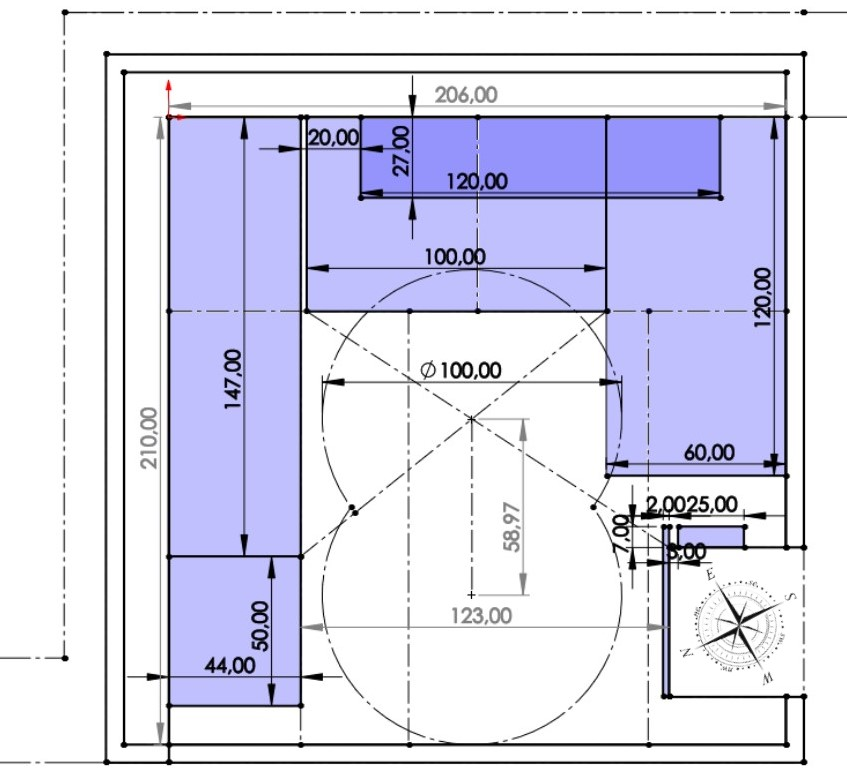
\includegraphics[width=0.9\textwidth]{./figuras/planos_caseta.jpg}
\caption{Diseño caseta, distribución mobiliario}
\label{F:planos_caseta}
\end{center}
\end{figure}

Dicha pared tiene de suelo a techo, mobiliario con cajoneras y estanterías, quedando el segundo nivel apoyado directamente sobre el medio alféizar. En el centro de la caseta se ha generado un espacio de 1-1.3 metros ideal para una silla giratoria con ruedas que accede fácilmente a toda la oficina y no entorpece el movimiento.

Por último tanto el espacio de entrada como los recovecos entre la chimenea-respiradero y el aluminio, son ampliamente funcionales debido a la puerta corredera y el uso de las pizarras este espacio es ampliamente usado como lugar de reflexión y pensamiento.

\subsection{Electricidad y Red}

La conexión eléctrica así como la conectividad se basa en una instalación nueva, extendiéndose desde la existente durante el proceso de puesta a punto previo a la instalación de armario y caseta. Con el objetivo de facilitar y separar las instalaciones, se dispondrá de un cableado de 2.5$mm^{2}$ y PIA asociado únicamente para la caseta y otro para enchufes e iluminación de terraza.

Inicialmente se contaba con un PLC de 10 Mbps que permite conexiones a través de la red eléctrica de iluminación de la terraza, sin embargo se ha instalado un cableado directo de ethernet desde la vivienda con el fin de maximizar dicha conexión a 1 Gbps.

\section{Construcción Oficina}

Este punto resume la construcción de la caseta presupuesto y tiempos aunque su detalle y pormenorizado se encuentra en el anexo \ref{S:anexo_B}.

\subsection{Acondicionamiento terraza}

Previamente a la instalación de la caseta así como del armario se realizaron un conjunto de tareas de acondicionamiento y mantenimiento previos que están descritos en anexo \ref{S:trabajos_previos} Los principales cambios fueron:

\begin{figure}[htb]
\begin{center}
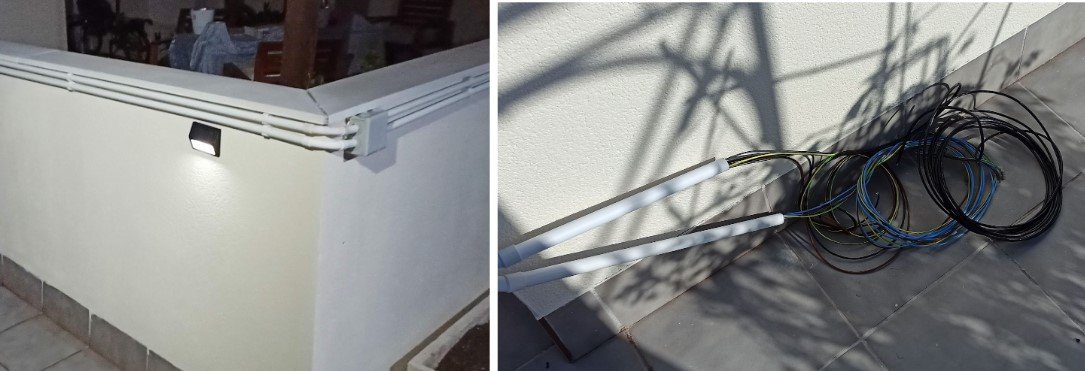
\includegraphics[width=1\textwidth]{./figuras/montaje_electrico.jpg}
\caption{Montaje eléctrico.}
\label{F:montaje_electrico}
\end{center}
\end{figure}

\begin{enumerate}
    \item Limpieza de paredes (barrido y agua a presión), alféizares con productos ácidos y suelos (con ácido clorhídrico diluido y detergente) para eliminar cal y abrir los poros.    
    \item Pintar la terraza y aplicaciones borada en juntas desgastadas entre baldosas.    
    \item Colocación de cajas y canalizaciones eléctricas en la terraza, permitiendo diferenciar, iluminación terraza, alimentación caseta y cable de red.
\end{enumerate}

\subsection{Caseta y armario}

El material de cortado así como montaje fue presupuestado y construido por una empresa local de aluminio, cerramientos, puertas y ventanas, que es la utilizada por la comunidad de vecinos para la instalación de las separaciones de medianera. En apenas 5 días la empresa encargada terminó la instalación completa de los cerramientos de aluminio, previos a la Semana Santa fig.\ref{F:estructuras_aluminio}
\begin{figure}[htb]
\begin{center}
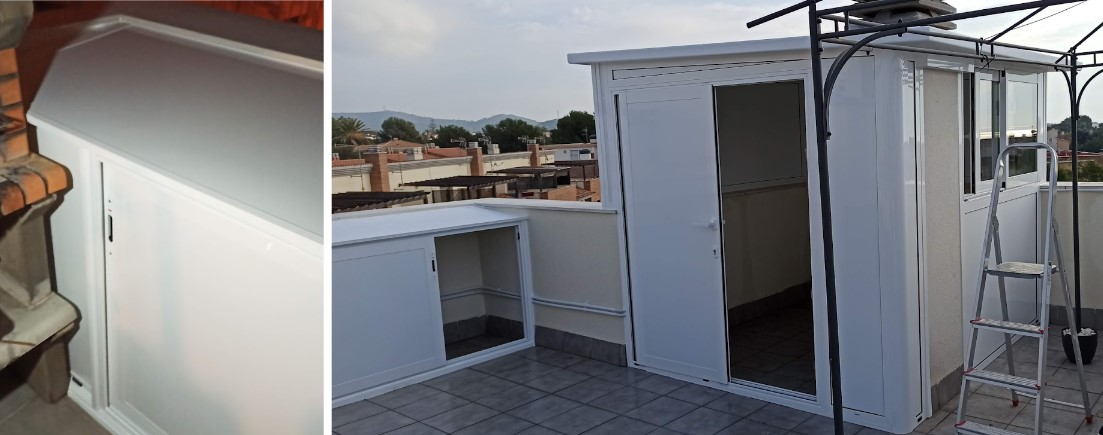
\includegraphics[width=1\textwidth]{./figuras/estructuras_aluminio.jpg}
\caption{Estructuras de aluminio.}
\label{F:estructuras_aluminio}
\end{center}
\end{figure}
En los días posteriores una vez secadas las juntas se continuó con la instalación eléctrica  tanto de armario como caseta, con puntos de luces, interruptores, enchufes y cajas internas fig.\ref{F:caseta_con_iluminacion_y_mobiliario}.
Así como un primer aislamiento de paredes y suelo con capa transparente anti-humedad previa a la colocación de mobiliario y alfombras.
\begin{figure}[htb]
\begin{center}
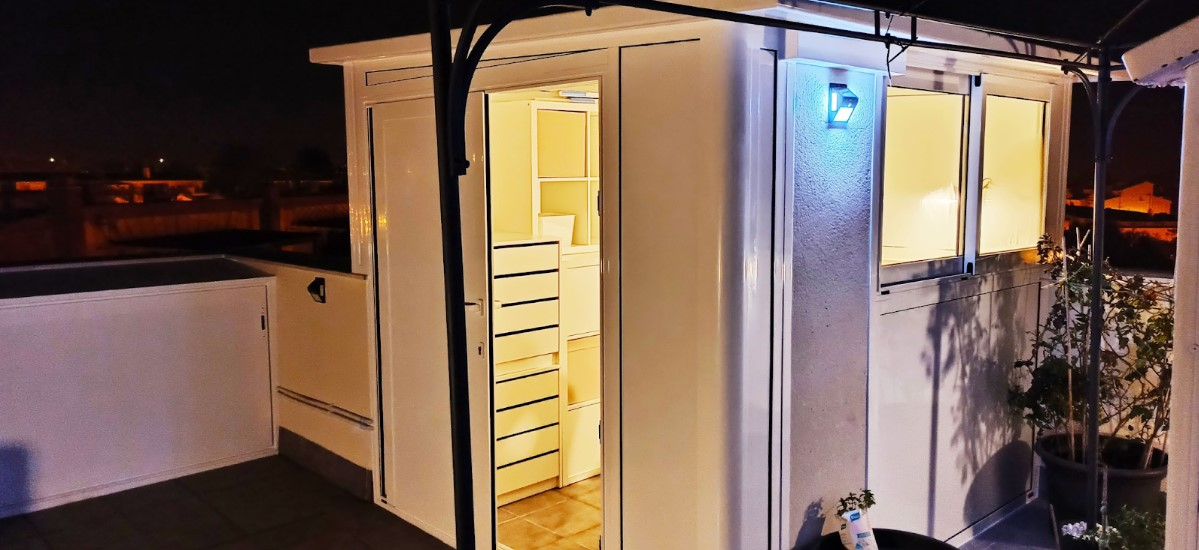
\includegraphics[width=1\textwidth]{./figuras/caseta_con_iluminacion_y_mobiliario.jpg}
\caption{Caseta iluminada}
\label{F:caseta_con_iluminacion_y_mobiliario}
\end{center}
\end{figure}
El mobiliario principalmente ikea o leroy merlin, se fundamenta en almacenamiento o estanterías apropiadamente seleccionadas para optimizar el espacio a un coste competitivo. La mesa y el elevador de pantallas son elementos estandarizados de ikea.
\begin{figure}[!htb]
\begin{center}
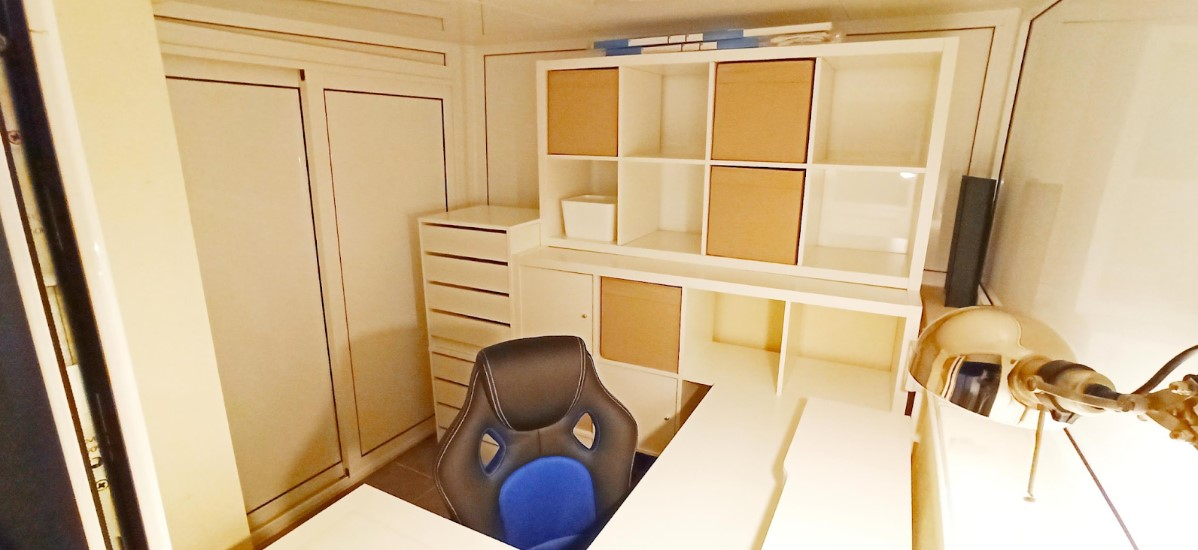
\includegraphics[width=1\textwidth]{./figuras/mobiliario_interior}
\caption{Caseta mobiliario.}
\label{F:mobiliario_interior}
\end{center}
\end{figure}

\subsection{Presupuestos planificación}

La gran mayoría de trabajos realizados a excepción de los montajes de aluminios se han realizado por este autor. Debido a ello la realización de las tareas no solo se ven limitadas por la secuencialidad de las mismas o necesidad de esperas como secado o asentamiento, sino que también se debe tener en cuenta que está mayoritariamente realizadas de viernes-domingo más días sueltos 4-6 h dedicados entre semana. Como contrapartida el coste real es “nulo” ya que no he asignado un precio real hora, pero como queda reflejado en la tabla de presupuesto con un tiempo personal muy monopolizado por la construcción.

Por ejemplo, aunque las tareas previas a la instalación de la caseta no superan los 15 días de trabajo continuado se realizaron durante Febrero-Marzo, casi 40 días laborales y 20 festivos.

\begin{figure}[!htb]
\begin{center}
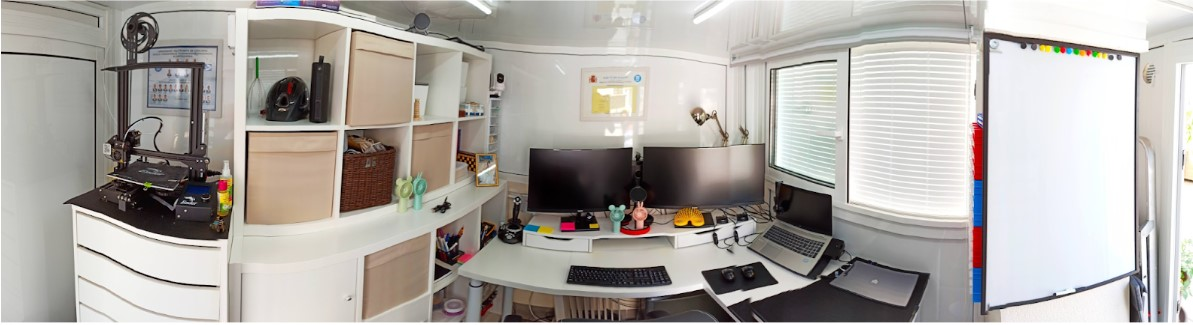
\includegraphics[width=1\textwidth]{./figuras/caseta_migrada}
\caption{Panorámica caseta migrada.}
\label{F:caseta_migrada}
\end{center}
\end{figure}
En la siguiente tabla se muestran los tiempos y costes de las tareas a realizar, que están dispuestas en orden cronológico de realización.
\begin{center}
\label{T:presupuesto}
\begin{longtable}[ht]{|p{3cm}|p{8cm}|p{1.5cm}|p{1.5cm}|}
\caption{Presupuesto Caseta Física}
    \\ \hline
    \textbf{Elemento} & \textbf{Descripción} & \textbf{Tiempo} & \textbf{Coste Material} \\ \hline
    Limpieza Alféizar & Barrer, frotar, aplicar producto limpieza especial, aclarado & 4 h & 6€ \\ \hline
    Limpieza Pared & Barrido y agua a presión & 1d & 0€ \\ \hline
    Limpieza Suelo & Barrido, fregado, limpieza con salfumán diluido & 1d & 10€ \\ \hline
    Pintar Terraza & pintado y limpieza posterior de suelo & 2d & 35€ \\ \hline
    Boradas y juntas & Aplicación y limpieza de borada en juntas. & 4d & 15€ \\ \hline
    Cajas y canalización & Colocación de cajas y canalizaciones eléctricas & 3d & 25€ \\ \hline
    Cableado Eléctrico & Pasar cableado eléctrico, interconexión de cajas y puntos de luz. & 2d & 40€ \\ \hline
    Cableado Ethernet & Adecuar cableado desde azotea comunitario, eliminar antena Wimax, pasar cableado por terraza. & 1d & 15€ \\ \hline
    Armario Aluminio Aislado & Montaje y sellado de armario por empresa. & 2d & 1500€ \\ \hline
    Caseta Aluminio & Montaje de laterales, montaje alféizar, montaje tejado, sellado. Montaje ventana y puerta. & 4d & 4500€ \\ \hline
    Luces, enchufes y tubos led & Instalación de cableado, enchufes, interruptores, cajas internas y tubos led de iluminación. & 3d & 60€ \\ \hline
    Mobiliario & Compra y montaje de mobiliario ikea & 2d & 450€ \\ \hline
    Mesa & Montaje de mesa customizada y eleva pantallas & 5h & 80€ \\ \hline
    Extras mobiliario & Separadores, protectores, cubetas ikea etc... & 1d & 60€ \\ \hline
    Pizarra & Montaje de pizarras en la chimenea-respiradero & 4h & 25€ \\ \hline
    Estore & Montaje y anclaje de estor interior difuminador de luz en ventana. & 2h & 20€ \\ \hline
    Mosquitera  & Instalar mosquitera plástica fácilmente reemplazable o reinstalable. & 1h & 4€ \\ \hline
    Persiana exterior & Compra instalación y sujeción de persiana alicantina externa de pvc. & 2d & 40€ \\ \hline
    Cámara Seguridad & IP cam con IA de reconocimiento personas con movimiento automatizado 360º & 2h & 35€ \\ \hline
    Alfombra Oficina & Alfombra robusta, oficina, con grosor extra aislante. & 2h & 80€ \\ \hline
    Mudanza & Mover el antiguo setup, herramientas, libros etc a la nueva oficina. Mover Impresora 3D, periféricos. & 3d & - \\ \hline
    Router & Router wifi para caseta y alrededores de terraza. & 1h & 25€ \\ \hline
    Switch & Switch Giga ethernet para conexiones por cable de elementos de la caseta & 1h & 20€ \\ \hline
    Google Home & Elemento interactivo de smart home dedicado a terraza y oficina & 1h & 18€ \\ \hline
    Smart things & Luces de terraza configurables (color, intensidad) accionadas por Alexa/Google assistant. Termómetro, interruptor inteligente. & 1h & 32€ \\ \hline
    Cámaras Seguridad & Cámaras de Seguridad Exterior de Terraza y Balcón, + Switch-Router que provee the conectividad a la terraza y las cámaras & 2h & 55€ \\ \hline
    Pingüino Calefactor & Pingüino, bomba calor/frió/deshumidificador para 15$m^{2}$ & 2h & 350€ \\ \hline
    ~ & ~ & ~ & ~ \\ \hline
    \textbf{Total} & ~ & \textbf{35d} & \textbf{7500€} \\ \hline
\end{longtable}
\end{center}

\subsection{Resultados de construcción}

Finalmente en mayo la caseta esta completamente terminada y 100\% funcional, siendo utilizada tanto en horario de oficina en mi trabajo, hobbies, formaciones y la elaboración de esta tesis. Así como la ejecución entre Febrero-Abril y un coste final de 7600-7800€, se puede asumir una finalización en plazo así como costes adecuados a lo planificado, no superando desvíos de 3-5\%.

\begin{figure}[htb]
\begin{center}
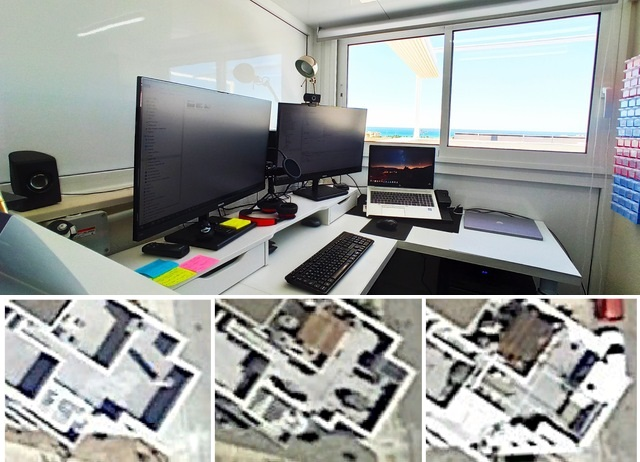
\includegraphics[width=0.9\textwidth]{./figuras/setup_mayo}
\caption{Setup en mayo, vista satélite pre pandemia, pandemia, actualidad.}
\label{F:setup_mayo}
\end{center}
\end{figure}

Véase una explicación al pormenor en el anexo B los puntos \ref{S:circunstancias} como la causa y comparativa con setups anteriores,  referentes a la construcción \ref{S:trabajos_previos}, \ref{S:estructura_aislamiento} así como otros puntos menos resaltables tales como iluminación \ref{S:iluminacion_caseta} y un conjunto no despreciable de fallos, mejoras y correcciones durante 2023 (\ref{S:cambios_2023}) que evidencian la continuación del proyecto mas allá de su desarrollo principal.

Por otra parte este proyecto de bricolaje técnico, ha servido de base para la aplicación en otros ámbitos personales del conocimiento técnico/practico adquirido, como la instalación del sistema eléctrico y solares en un almacén agrícola de mi padre; el cableado ethernet de mi casa, casa de mis padres, suegra, oficinas y en general cualquier amigo que me ha pedido ayuda con cableado ethernet y cámaras de seguridad. Así como muchos elementos del setup, y especialmente la guía\cite{c_guia_hardware} y a previsión de mantenimiento para la selección de hardware con fines profesionales a largo termino.

Finalmente como cliente y promotor de este espacio, me siento completamente satisfecho al pasar una media entre 9-13 horas de mi día a día en dicho espacio y obtener un aislamiento familiar perfecto y separación de entorno profesional y personal.

\chapter{Servicios y herramientas}\label{S:tema_2}
Una vez resuelto los temas propiamente físicos, es necesario evaluar las diferentes posibilidades, softwares y estrategias para permitir realizar un trabajo virtualmente. Este tema muestra los diferentes puntos de interés a la hora de generar una nube y sus diversas herramientas necesarias para el día a día.

\section{Software, hardware y gestión.}
En el Anexo \ref{S:decisiones_software} se especifica el razonamiento tanto de las licencias como del tipo de software base que se utiliza en esta oficina virtual. 

El precepto es el uso de \textbf{Software libre, auto gestionado}, generalmente basado en versiones \textbf{LTS(Long Time Support) soportadas por comunidades} que dependiendo de un análisis coste/precio se auto gestiona o externaliza parcialmente.

Por ello aunque el 98\% de la utilidades y necesidades pueden ser cubiertas por software libre desde el SO (Sistema Operativo) linux, tareas ofimática y especialmente en desarrollo de software, se entiende que una licencia retail tanto de windows, como programas genéricos de ofimática puede no superar los 3-10€ siendo permanentes y fácilmente asequibles, especialmente cuando hablamos de pc/laptop desktop y no de servidores. 


Respecto a que auto gestionar y que externalizar, adoptaremos un enfoque puramente económico, minimizando los costes en base a nuestro conocimiento técnico. Por ello la principal externalización son el dominio y servidor de correo, junto a uno/dos VPS (virtual private server), como punto externo de conectividad para aplicaciones esenciales véase anexo \ref{S:anexo_mvp}, donde también se detalla el aprovisionamiento y securización anexo \ref{S:setup_abastecimiento}.

\begin{table}[!ht]
    \centering
    \begin{tabular}{|p{4cm}|p{5cm}|p{5cm}|}
    \hline
        \textbf{Requisito} & \textbf{Caso seleccionado} & \textbf{Coste} \\ \hline
        Hardware cloud base & VPS (2 cpu, 2GB/44G ram, 40 GB disk, red  250/500 Mbps) & 4-6 € / mes (dependiente de promoción) \cite{c_vps_ovh} \\ \hline
        Hardware cloud productos & VPS (2/3 cpu, 4GB ram, 80 GB disk, red  500 Mbps) & 8-12 € / mes (dependiente de promoción) \cite{c_vps_time4vps} \\ \hline
        Hardware Desarrollo & power hardware wake up on demand ( localhost ) & 20-40 € / mes coste eléctrico \\ \hline
        S.O (base) server & Linux LTS: Debian, Alma o Rocky & 0€ LTS community supported \\ \hline
        Cloud platform & Ansible \& docker \& docker-compose/swarm  & 0€ LTS community supported \\ \hline
        Services & Principalmente servicios auto alojados mediante dockerizacion & 0€ community supported \\ \hline
    \end{tabular}
\end{table}

\section{Ansible}
Ansible\cite{c_ansible} es uno de los software más utilizados actualmente como herramienta devops,  y es la principal herramienta de automatización de este trabajo. Ansible es un software de aprovisionamiento y orquestación, es decir, permite gestionar configuraciones y tareas orientadas a estado de una manera simple y centralizada.

La herramienta utiliza SSH para comunicarse desde un nodo central, utiliza YML como lenguaje descriptivo y JSON como salida. Permite usar una gran variedad de módulos para realizar tareas simples.
\begin{figure}[!htb]
\begin{center}
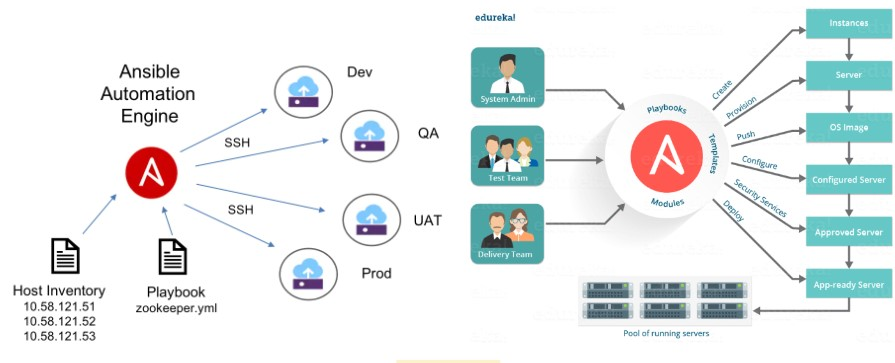
\includegraphics[width=1\textwidth]{./figuras/ansible_diagram.jpg}
\caption{Ansible diagrama funcionamiento\cite{i_ansible_1}\cite{i_ansible_2}.}
\label{F:ansible_diagram}
\end{center}
\end{figure}
El objetivo de la herramienta es generar grupos o jerarquías de servidores a los que conectarse vía SSH con los credenciales apropiados. Nótese que no es necesario de ningún software previo en dichos servidores únicamente un servicio SSH con la apropiada credencial de login.
\begin{figure}[!htb]
\begin{center}
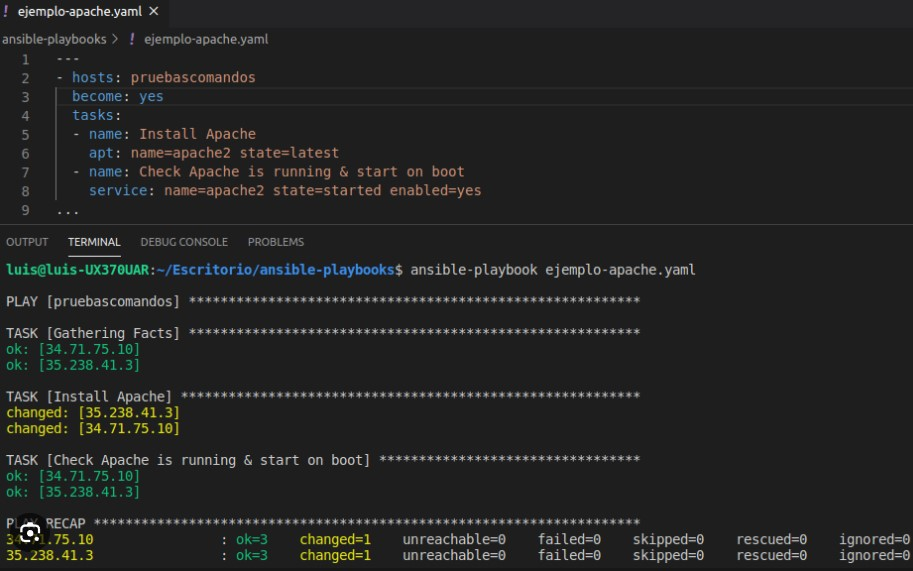
\includegraphics[width=0.9\textwidth]{./figuras/ejemplo_ansible.jpg}
\caption{Ansible ejemplo de ejecución desde proyecto VScode .}
\label{F:ejemplo_ansible}
\end{center}
\end{figure}
Una vez conectado ejecuta el comando o las tareas asociadas al script de ejecución (copiar configuraciones, ejecutar comandos, verificar estados). Estas tareas están sujetas a estado, es decir, el YML de la tarea define el estado final que se desea y el script chequea si se cumple o sino ejecuta la tarea para obtenerlo. Las tareas se ejecutan por grupo y/o tag y la ejecución se produce en paralelo en todas las máquinas.

El resultado final es que tras la ejecución del script, recibimos un output coloreado no solo con las descripción de las tareas verificadas, ejecutas  y resultado de las mismas sino con la posibilidad de acceso a un log detallado en formato json (véase fig.\ref{F:ejemplo_ansible}).

El verdadero poder de los módulos de Ansible reside en su gran abanico de opciones y softwares soportados. Permitiendo gestionar host virtualizadores o API de proveedores para crear máquinas, dispositivos de red. Ejecutar o acceder la casi totalidad de las funciones de linux y windows server. Configuración y ejecución de software de amplio uso como docker\cite{c_docker}, kubernetes\cite{c_kubernetes}, git\cite{c_git}, npm, gestores de repositorios o librerías, y la retroalimentación del output de ciertas tareas para la designación de tag o grupo de la máquina ejecutora o como input condicional para otras tareas.

Finalmente Ansible también permite la agrupación de las tareas y ficheros relacionados como rol en una estructura jerárquica de ficheros. Por lo tanto, automatizar una tarea como 'rol'. Esta estructura facilita su puesta en marcha, su actualización y su publicación en Ansible Galaxy (repositorio de rols de ansible), o lo que es lo mismo re-utilizar la gran cantidad de publicaciones de rol, evitando tener que crear un trabajo desde cero o tener acceso a innumerables ejemplos reales.

Debido al acoplamiento del caso real (Elenkar) y la sensibilidad de ciertos datos, sensibles desde el punto de vista de seguridad hacia futuros ataques, solo se han desvelado parcialmente las partes mas genéricas de dichos script, véase anexo \ref{S:ansible_ejemplo} como ejemplos.

\section{Contenedores y Docker Service}
Cuando se necesita ejecutar una aplicación o servicio se necesitan tres cosas principales, un SO que lo soporte, las librerías externas que pueda usar el software y la configuración e instalación customizada dentro del SO que lo ejecuta.

A excepción de software auto empaquetado como el de Mac OS o aplicaciones snap, la gran mayoría de softwares utilizan librerías (dll, lib) para su funcionamiento (“reusar es de pobres, pero eficiente” ). La gestión de las librerías puede conllevar a un problema cuando múltiples aplicaciones del SO requieren de librerías que entran en conflicto, o dejan de ser soportadas tras una actualización o los requisitos de máquinas virtuales de ejecución Python, Java, Php, Node, requieren de diferentes versiones en paralelo.

La necesidad de gestionar servicios pseudo duplicados que actúan sobre un mismo puerto (apache, tomcat, node) o el uso compartido de varias aplicaciones del mismo host-web. No solo hace complejo su gestión sino vulnerable ya que afecta a todos los elementos de manera transversal. La caída del servicio base o la vulneración de seguridad de una aplicación puede exponer el resto de ejecuciones del SO al compartir sistema de archivos, procesos y memoria; y solucionar este problema por VM (Máquinas virtuales) por servicio es poco eficiente y económicamente costoso.

\begin{figure}[!htb]
\begin{center}
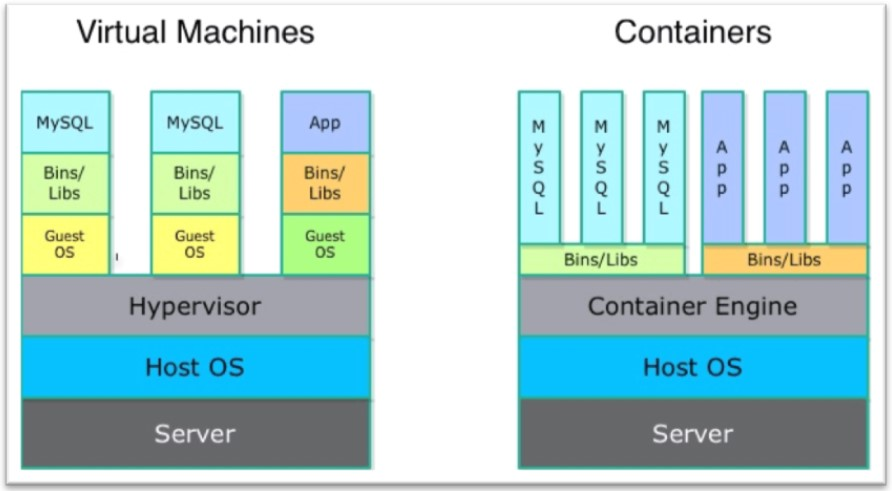
\includegraphics[width=1\textwidth]{./figuras/virtual_machine_vs_docker.jpg}
\caption{Maquina virtual vs contenedores\cite{i_containers}.}
\label{F:virtual_machine_vs_docker}
\end{center}
\end{figure}
Un contenedor, no es más que un formato estandarizado que incluye la aplicación, sus dependencias y una base de sistema operativo, para una ejecución independiente, aislada y ligera de la aplicación. A diferencia de una Virtual machine, el contenedor no emula hardware, sino que ejecuta la aplicación directamente en el kernel del sistema hospedante, sin embargo utiliza la abstracción a 'nivel de espacio de usuario' (similar chroot, cgroups y namespaces\cite{c_funcionamiento_docker}) para que el sistema de archivos, los recursos, los procesos estén aislados en el contenedor. Por otra parte, los contenedores usualmente contienen un único hilo de ejecución que es arrancado al iniciar el contenedor y cuyos cambios no son persistentes, sólo temporales mientras el contenedor está en ejecución.

Docker\cite{c_docker} es un software de código abierto usado como servicio de contenedores. Permite crear, gestionar, abstraer y automatizar el uso de contenedores permitiendo definir redes, puertos, arrancar imágenes, acceder a sus logs o mapear carpetas persistentes dentro del container.

Las imágenes de un container se crean en base a capas (como fotos del sistema de archivos), de tal manera que múltiples imágenes de aplicaciones diferentes pueden compartir capas. Si tengo múltiples imágenes de contenedores, que ejecutan software java, pero el SO (alpine) y la máquina virtual de java son iguales únicamente las capas diferentes, dependencias y aplicación serán propias de cada container. De igual manera la diferencia entre las imágenes y los container en ejecución es una última capa temporal que contiene los cambios del contenedor durante su ejecución. Entendiendo esta propiedad; es factible ejecutar múltiples containers de una misma imagen en paralelo, es decir, permite el escalado horizontal de recursos.

Por último las imágenes se pueden almacenar en repositorios como Docker Hub, que sirven a su vez no solo para arrancar contenedores sino como base para imágenes más complejas, permitiendo desarrollar tus imágenes únicamente dependientes de la capa de aplicación y delegando en comunidades el mantenimiento de aquellos elementos que no son el focus de nuestro producto.

Las principales mejoras de usar docker son:
\begin{itemize}
    \item Aislamiento, seguridad, gestión simplificada centralizada de múltiples aplicaciones dockerizadas en una única Virtual machine / servidor.
    \item Rapidez, simplicidad y sencillez en despliegue sin necesidad de instalación.
    \item Administración del sistema, sin conocimiento previo o mantenimiento sobre la aplicación.
    \item Consistencia e Independiente de plataforma, misma ejecución en test, local o producción. Facilidad en pruebas o despliegues continuos (CI/CD).
    \item Modularidad y escalabilidad horizontal, perfecto para entornos de microservicios o ambientes distribuidos.
    \item Repetibles, replicables y versionables, permite facilitar las migraciones o flexibilizar entornos y desarrollos muy ágilmente.
\end{itemize}

Por ultimo se debe entender que con el énfasis de la automatización, muchos de nuestros servicios dockerizados necesitan acceder a información de otros servicios dockerizados, por lo que en este documento se utilizan aproximaciones de docker complejas ( dind o dood) ve ase Anexo \ref{S:docker_complex}

\section{Docker Compose, Kubernetes, Docker Swarm}
Existen múltiples orquestadores sobre docker. Un orquestador de container es una capa extra de software que interacciona con nuestro engine de contenedores. Su principal ventaja es la configuración o el acceso a una interfaz más humana que el command line del engine. 

\begin{figure}[!htb]
\begin{center}
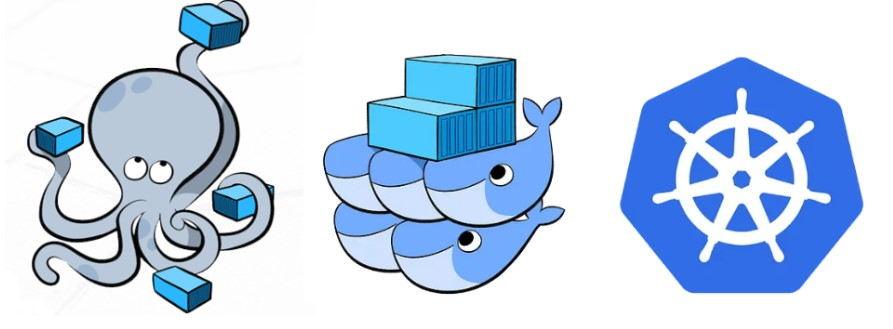
\includegraphics[width=1\textwidth]{./figuras/docker_compose_swam_kubernates.jpg}
\caption{Docker compose, swam y kubernetes logo images\cite{i_orquestadores}.}
\label{F:docker_compose_swam_kubernates}
\end{center}
\end{figure}
Sin embargo otras tareas como la definición de relaciones entre contenedores, sincronía y monitorización también son añadidas a la propia funcionalidad del engine. El mejor ejemplo es Docker-Compose\cite{c_docker_compose}, que permite configurar fácilmente en un formato YML multiples contenedores, redes, volúmenes, condiciones y relaciones entre ellos en un único fichero, permitiendo su arranque y gestión. Docker-Compose es el orquestador utilizado en este documento debido a su facilidad y el foco de una única máquina (VPS) o servidor autocrático, que actúa de manera aislada.

Sin embargo, si fuera necesario, Docker-Swarm\cite{c_docker_swarm} es un orquestador que incluye las funcionalidades de docker-compose y genera un cluster de trabajo, permitiendo unificar múltiples máquinas con servicio docker instalada como un único cluster. Facilitando no solo las herramientas de un cluster tales como master-slave, backups y balanceo de carga, sino añadiendo más herramientas no incluidas en docker-compose, como escalado, monitorización, ingress network point y encriptaciones .

Por último Kubernetes\cite{c_kubernetes} es un framework de containers, open source creado por google, que gestiona de una manera más profunda y profesional la creación y uso de un cluster de contenedores en la nube. Aunque es mi herramienta diaria de trabajo como desarrollador de software, no será usada en este trabajo puesto añade un complejidad y trabajo adicional no necesario para el nivel de requisitos de nuestros servicios donde \textbf{no se espera una gran demanda y se tiene una restricción de recursos escasos}.

\section{Arquitectura de nuestros Servicios}
La arquitectura base de la oficina virtual se fundamenta en la conjunción de tres pilares:
\begin{figure}[!htb]
\begin{center}
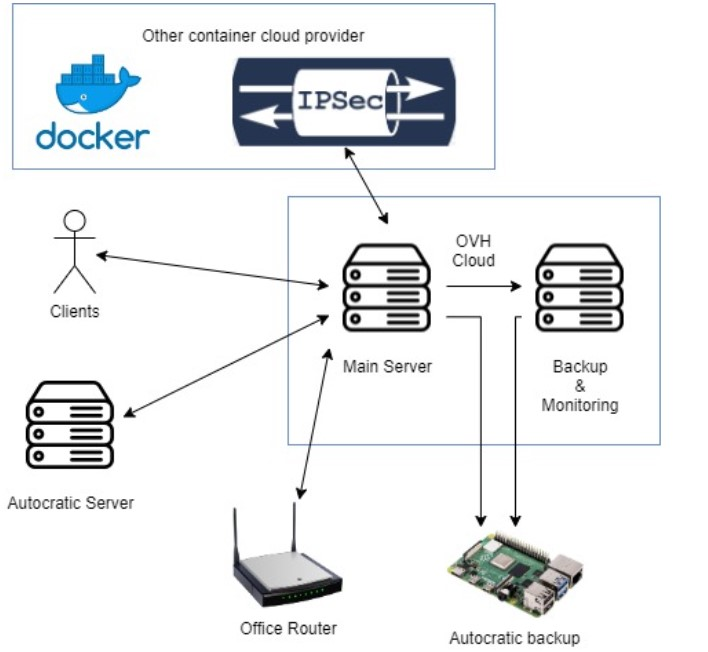
\includegraphics[width=0.75\textwidth]{./figuras/arquitectura.jpg}
\caption{Diagrama de interacción.}
\label{F:arquitectura}
\end{center}
\end{figure}
\begin{itemize}
    \item Uso de Linux LTS segurizado y automatizado que instala docker como principal servicio, minimizando y facilitando el mantenimiento de la máquina.
    \item El uso de docker y orquestadores de docker para proveer de los diferentes servicios necesarios y la interacción de los mismos.
    \item El uso de Ansible para el aprovisionamiento del servidor, la seguridad y configuración de los servicios, asi como la conetividad y configuraciones de elementos conectados al VPS por una VPN o túneles.
\end{itemize}
Los servicios públicos tales como web publica, proxy o vpn son expuestos directamente.

El servidor principal, permite conexiones reversas a los servidores-granja de producto o servidores autócratas re-enrutando el trafico. Un servidor secundario sirve como gestor de mantenimiento, monitorización y backup del principal, así como un backup autocrático en local con raspberry pi almacena el histórico de backups y configuraciones.

En todo momento, la idea es poder crecer en una nube externalizada o local, así como mantener en todo momento un control de backup. El proxy permite exponer servicios hospedados en nube externa o local a través del servidor principal VPS. La VPN permite conectar a servicios no expuestos a internet, pero si en la intranet.

Todo ello fácilmente gestionable por ansible, docker-compose que junto a los backups de configuraciones y volúmenes permiten replicar, migrar o restaurar todo en cuestión de minutos.

\section{Aprovisionamiento y Securización}
El aprovisionamiento principal es configuración, creación de grupos, permisos, eliminación de todo software innecesario del servidor, añadir docker, actualizaciones desatendidas y la autorización de claves ssh sobre un usuario administrativo de deploy.

La principal baza de seguridad de este proyecto se basa en la simplicidad, aislamiento y el uso de docker como elemento separador entre aplicaciones.

Por lo tanto, blindando del firewall y servicio SSH, la seguridad se basa en la ausencia de “accesos” y la “compartimentación”  de elementos. A excepción de los servicios públicos dockerizados y SSH no hay más servicios expuestos en la ip pública del VPS aislando y protegiendo el SO. Así mismo aquellos servicios que no requieren de ser expuestos públicamente, se utilizan internamente vía vpn - intranet.

Por lo general se puede resumir la securización del server en los siguientes conceptos:
\begin{enumerate}
    \item Purga de elementos vulnerables o no usados del sistema.
    \item Denegación de todo puerto no autorizado. Firewall ofensivo con denegación de ip.
    \item Configuración securizada de ssh. Solo permitidos non-root, vía claves asimétricas y valores default cambiados.
    \item Control con filelog, logwatch, logcheck, accounting para auditorias.
    \item Log rotate, y mecanismo de mitigación de ataques como fail2ban o denyhosts.
    \item Exponer el mínimo de servicios externamente y usar VPN para el resto.
    \item Scripts de control, sudo limitado y notificaciones de procesos de superusuarios.
    \item Usar VPN e integrar una nodo (raspberry pi o similar) con NIDS (Network Intrusion Detectors System) como prevención en redes locales interconectadas.
    \item Usar imágenes docker oficial o auto-ensambladas, que siguen buenas prácticas o escáneres de seguridad (docker hub lo incluye).
\end{enumerate}

Véase rol del Ansible de segurización \cite{c_code} y el anexo \ref{S:anexo_segurizacion} .

\section{Servicios}
En este apartado se indican los servicios seleccionados como nube MVP(Minimum Viable Product), en el anexo  \ref{S:anexo_mvp} se detallan razonamiento, posibles candidatos y una argumentación sobre cada uno de los principales servicios. En la tabla ~\ref{T:mvo_mas_diez} y  ~\ref{T:mvp_nube_seleccionado}, indican como obligatorios los marcados con un a ’*’. En el caso de que la nube se aplique a un grupo de trabajo de 10 o mas personas se incluyen los siguientes servicios:
\begin{table}[!htb]
\caption{Docker services más de 10 personas.}
\label{T:mvo_mas_diez}
\begin{tabular}{|p{2cm}|p{3cm}|p{5cm}|p{2cm}|}
\hline
\multicolumn{1}{|c|}{\textbf{Tipo de Servicio}} & \textbf{Herramienta} & \multicolumn{1}{c|}{\textbf{Detalles}} & \multicolumn{1}{c|}{\textbf{Tipo y Coste}} \\ \hline
Comunicación Interna \textgreater{}10 trabajadores & Rocket Chat\cite{c_rocket_chat} & Requiere recursos y mantenimiento continuado, es decir, servidor dedicado & Interno VPS dedicado 3-5€ / mes \\ \hline
Autenticación Centralizada & KeyCloak\cite{c_keycloak} con LDAP\cite{c_ldap} & Utilizar un LDAP que suministra información a KeyCloak y automatizar la carga de LDAP & Interno 0€ VPS principal \\ \hline
\end{tabular}%
\end{table}

\begin{table}[!htb]
\caption{Servicios docker nube MVP.}
\label{T:mvp_nube_seleccionado}
\begin{tabular}{|p{2cm}|p{3cm}|p{5cm}|p{2cm}|}
\hline
\multicolumn{1}{|c|}{\textbf{Tipo de Servicio}} & \textbf{Herramienta} & \multicolumn{1}{c|}{\textbf{Detalles}} & \multicolumn{1}{c|}{\textbf{Tipo y Coste}} \\ \hline
Correo Electrónico * & Don Dominio\cite{c_dondominio} & Externo 10 € / año 10 cuentas 3 GB o 20 € / año 15 cuentas 10 GB. & Externo 10 € / Año \\ \hline
Comunicación Externa* & Teams, Zoom, Whatsapp, Telegram & Centralizadas desde cliente Fermi. & Externa, 0€ \\ \hline
Comunicación Interna & Teams / Slack & Es un elemento excesivamente costoso, en recursos. Se usara servicio gratuito limitado. & Externa, 0€ \\ \hline
Almacenamiento* & Nextcloud\cite{c_nextcloud} & Requiere recursos, es decir, servidor VPS dedicado o via intranet a un server autocratico. & Interno 3-5€ / mes \\ \hline
Aplicación ofimática & Only Office / collabora\cite{c_colabora} & Hosteado junto a next cloud en un server dedicado. & Interno incluido nextcloud server \\ \hline
Wiki* & Bookstackapp\cite{c_bookstack} / MediaWiki\cite{c_media_wiki} & Ligero y útil para desarrollo. & Interno 0€ VPS \\ \hline
VPN* & Wire Guard\cite{c_wireguard} & Punto externo de conexiona intranet, generación de múltiples VPN. & Interno 0€ VPS \\ \hline
Repositorio de Code & Gitea\cite{c_gitea} & Si es publico en servidor VPS principal, si es privado puede estar en un server autocrático. & Interno 0€ VPS \\ \hline
CI/CD & Jenkins\cite{c_jenkins} / Drone \cite{c_drone}& Si es publico en servidor VPS principal, si es privado puede estar en un server autocratico. & Interno 0€ VPS \\ \hline
Web Service* & WordPress\cite{c_wordpress} / Static web\cite{c_hugo} & Simplemente como pagina web principal y/o blog & Interno 0€ VPS \\ \hline
Ticketing & Taiga\cite{c_taiga} & Simple y eficiente board de scrum-agile. & Interno 0€ VPS \\ \hline
\end{tabular}%
\end{table}

Es importante recordar que en las pruebas de concepto anexo \ref{S:pruebas_concepto} no se ha automatizado el proceso de configuración de interacción entre los servicios, en el caso de autenticación. 

El tuning de los plugins o las third parties, debe hacerse manualmente durante la primer arranque de la nube. Este proceso puede automatizarse pero requiere un conocimiento específico de cada servicio y tiempo dedicado excesivo, por lo que se ha priorizado la prueba de múltiples servicios y la selección del más conveniente, ya que una vez configurado apropiadamente, puede usarse el primer backup como producto pre configurado de la nube. 

Finalmente recordar que no es necesario el uso de todos los servicios, es decir, la empresa u oficina virtual debe hacer uso en función de sus necesidades, tanto en tamaño de grupo de trabajo, criterios de seguridad y monitorización etc ... deben ser coherentes con las necesidades.
\clearpage

\section{Múltiples Docker compose y limitaciones}
Para la puesta en marcha tanto de servicios externos, así como servicios no expuestos debemos de entender que muchos de ellos tiene bases de datos o servicios auxiliares, es decir por ejemplo el servicio de web puede ser un único container con todo (db,wordpress,web server, php) o puede ser múltiples container aportando cada uno su propio sub-servicio. Por lo tanto ya sea por catalogación o por simplicidad no es práctico la generación de un único docker-compose con todos los servicios. 

Lo óptimo es la definición de servicios o grupos de servicio bajo un único docker-compose, facilitando la tarea de instaurar un servicio systemD\cite{c_docker_compose_systemD} de Linux, que arranque los servicios junto con el Sistema operativo. Otro elemento útil es el uso de “Múltiples file call”\cite{c_docker_compose_multiples} en casos complejos o de elementos comunes permitiendo importar sub-ficheros yml para conformar un docker-compose final o sobre-escribir un fichero con otro \cite{c_docker_compose_override}. Par aun mayor detalle véase anexo \ref{S:docker_compose_details}.

La principal limitación de docker-compose es su aplicación en un único host, lo que limita su uso a entornos de desarrollo/testing o como nuestro caso aquellas herramientas que no requieren de una alta disponibilidad y demanda, ya que no implementa de manera nativa ningún tipo de escalado o balanceo de carga. Sin embargo si utilizamos versiones superiores a la V3, es plausible deployar directamente ficheros docker-compose en cluster de docker swarm previamente inicializados facilitando la evolución hacia un escalado horizontal de recursos.

\section{Docker Backups}
Como se ha mencionado en el anterior punto, se ha priorizado la configuración manual de plugins o interrelaciones entre los servicios, sobre la “auto-creación por script” ya que requiere de un tiempo y esfuerzo sobre dimensionado para el objetivo de este trabajo, que es tener una nube, pero no auto-configurar ágilmente.

Sin embargo sí es objetivo que esta nube se pueda construir y destruir o realizar una restauración ágilmente, es decir, se definen y configuran las relaciones entre servicios, se realiza un backup que puede ser usado como base de construcción para nuevos despliegues (siempre y cuando se mantenga la selección de servicios e interrelación). Por lo tanto la generación de backups periódicos para posibles restauraciones, así como el despliegue de backups como nuevas nubes es un elemento obligatorio.

Toda la información que los servicios desplegados contienen se fundamenta en las capas variable de los contenedores y en los volúmenes persistentes, es decir, con el apropiado backup de volúmenes, los contenedores son capaces de re-arrancar con todo apropiadamente configurado. 

Muchas veces los servicios dependen de otros servicios auxiliares tales como bases de datos, en estos casos dependiendo de si se aplicado una política de centralización en una única base de datos o en múltiples, puede hacerse el backup “por servicio” exportando sus schemas, o realizarse directamente un backup del volumen de la ddbb.

En todo caso el procedimiento siempre sigue una pauta marcada, que únicamente es influenciada por los recursos que disponemos en el VPS:
\begin{enumerate}
    \item Parada de servicios, excepto ddbb o similares.
    \item Backup de ddbb o servicios auxiliares por script.
    \item Apagado de todo servicio y realización de backup de volúmenes.
    \item Reiniciado de servicios.
\end{enumerate}


El punto crítico es la capacidad de procesado así como el espacio limitado en disco. 

Existen múltiples puntos de vista a la hora de realizar el backup usualmente se utilizan métodos de diferenciado binario con checksum (similar a git) y compresión para generar layers de cambio de las que se almacena un número máximo de veces. 

Existen software especializados también dockerizados como autorisc\cite{c_autorisc} o duplicati\cite{c_duplicati}, sin embargo el punto principal de este backup en el VPS es minimizar el uso de recursos por ello se sobreentiende que verdaderamente el backup es una sincronización en red, utilizando software como rsync\cite{c_rsync}, que sincroniza los folders de los volúmenes con un servidor remoto y es allí donde se realiza el proceso de backup propio y almacenado del último backup en un medio donde la capacidad no es un problema, ni existen limitaciones de cpu.

Entiéndase también que la realización del backup es automática-global, aunque se permita por la estructura de carpetas y subcarpetas la realización parcial de backup manualmente. 

\section{Automatizaciones y scripts}
Una vez seleccionados los servicios necesarios para nuestra nube y su prueba de concepto validada, es necesario la realización de automatizaciones para su uso diario y gestión:
\begin{itemize}
    \item Ansible y script de despliegue, son principalmente scripts de ansible que deben permitirnos un despliegue rápido desde cero de todos nuestros servicios. Dicho despliegue debe validar y llamar a script de securización y aprovisionamiento si las máquinas elegidas, si no están apropiadamente predispuestas.
    \item Apagado, encendido de la plataforma, haciendo énfasis en la automatización de muchos servicios o grupos de servicios como servicio de systemd\cite{c_systemd}, incluyendo la inicialización de los mismo al reiniciar la máquina linux  (véase anexo \ref{S:systemD} ).
    \item Cron, script o ansibles de backups, purgado de datos y chequeos de seguridad y actualización. Su principal función es verificar la seguridad y consistencia de las máquinas linux, gestionando un apagado para la realización de backups, limpieza y reinicio de la plataforma principalmente en horario nocturno (3-5 am).
    \item Validación de ecosistema, los anteriores apartados hacen referencia a máquinas exclusivamente centradas en VPS o servidores, pero es necesario una validación y gestión del cloud en todas las características añadidas, redes, conexiones vpn a otros servidores o entornos de trabajo.
\end{itemize}

\section{Legalidad}
Este apartado indica únicamente una tendencia o recomendaciones a la hora de evaluar los requisitos y riesgos legales de nuestra nube. Como ciudadanos europeos o empresas que trabajen dentro de el área económica europea, debemos tener claro 2 pilares fundamentales:
\begin{itemize}
    
    \item Cumplir la carta de derechos fundamentales de la UE y directivas o reglamentos europeas de protección de datos\cite{c_ue_rpgd}, ya que estas incluyen las leyes nacionales\cite{c_boe_rpgd} de los diferentes estados en temas de protección de datos, derechos u obligaciones en el mundo digital europeo.
    
    \item Servidores europeos o equivalentes, es decir, muchos de los requisitos necesarios se adquieren al usar un proveedor europeo con sede en Europa, o en países homologados para datos europeos. Este punto es especialmente conveniente, debido a que raramente se utilizan nubes lejanas geográficamente debido a la degradación de propiedades de red como el ping, availability, bw que degradan la conexión.
    
\end{itemize}

La recomendación como desarrollador que impera, para evitar la complejidad y el sobre esfuerzo de tratar con datos sensibles, es "\textbf{utiliza única y exclusivamente aquellos datos realmente necesarios"}, haciendo especial énfasis en evitar aquellos datos de especial sensibilidad como religión, tendencia sexual, etnia, afiliaciones políticas o sindicales, genéticos, biométricos identifica-torios, relativos a historial de salud o datos traceable.

La segunda recomendación es no vincular datos personales con otros conjuntos de datos almacenados, facilitando la eliminación de los mismos en el plazo de conservación de los datos de carácter personal.

La tercera recomendación es, segmenta, clasifica tus datos o modifícalos degradando su sensibilidad. Degradar o hacer anonimo un dato significa implica tener un dato sensible como la MAC, IP u otros identificadores que por su carácter único y identificativo es necesario. Se pueden transformar vía hash o checksum obteniendo un segundo valor que no tiene las clasificación de datos personal pero mantiene su carácter único y traceador para nuestro aplicativo.  

\subsection{Clasificación de datos e inventario}
Es importante inventariar y clasificar los datos utilizados en la nube o software. Se recomienda una clasificación a tres niveles:
\begin{enumerate}
    \item Confidencial: un dato que requiere no ser expuesto y por lo tanto no puede almacenarse en claro. Limitando el acceso al valor.
    \item Activo critico: es un dato confidencial con integridad y 'availability', es decir, permite verificar su no modificación y un procedimientos de acceso garantizado.
    \item Datos personales identificables, es un activo critico de carácter personal, por lo que incluye una clausula de tiempo de almacenamiento y eliminación el tiempo máximo legal.
\end{enumerate}

\subsection{Consentimiento y mecanismo de acceso}
Cuando obligatoriamente necesitamos un dato sensible, es muy importante que el tratamiento se base en el consentimiento del interesado, el responsable deberá ser capaz de demostrar que aquel consintió el tratamiento de sus datos personales. Por lo tanto el consentimiento debe ser inequívoco y explícito, ya que tiene la responsabilidad jurídica de demostrar que el usuario ha dado su permiso. Como ejemplo \textbf{no se puede poner pre-marcado por defecto la aceptación de política de privacidad}.

Por otra parte en todo momento existen unos procedimientos\cite{c_aedp} para atender las demandas de los clientes sobre sus derechos, y dichos procedimientos deben ser visibles, accesibles y sencillos.
\chapter{Redes y Casuísticas}\label{S:tema_3}
Este tema resume y expone ejemplos llevados a cabo en la prueba de concepto de redes para la oficina virtual. Es de especial interés para comprender el detalle realizado la lectura del Anexo \ref{S:anexo_D}.

\section{VPN e intranet}
Primeramente hemos de entender que siempre existe una “red común”, por lo tanto ya sea como freelance en mi oficina en casa, o la sede física de una pequeña pyme o una gran oficina en un edificio de cristal en el centro metropolitano, o una red en un cloud siempre existe una \textbf{red principal}.

\subsection{Objetivos de VPN}
Normalmente los servicios internos están accesibles dentro de esta red y bloqueados externamente. Por lo tanto tenemos múltiples intereses para implementar una VPN o virtual private network, comúnmente llamadas intranet, que nos permita el acceso a esta red interna:
\begin{itemize}
    \item Conexión directa con otros elementos de la VPN, es la funcionalidad básica de una red, permite interconectar pc, impresoras o varias personas, pero usando una interfaz virtual, es decir, cada uno usando como soporte su LAN-real.\textbf{ Especialmente interesante para utilizar elementos de control remoto} o monitorización.

    \item Conexión entre redes, en muchos casos puede ser de interés que múltiples LAN (múltiples sedes) sean también accesibles entre sí mediante la red principal sin necesidad de ser expuestas a internet o alquilar un cable-túnel a un proveedor de telecomunicaciones.
    \item DNS, monitorizado y filtrado. Especialmente útil para monitorizar. Usualmente las redes tienen su propio dns, que aparte de añadir servicios interno, permite filtrar llamadas dns o implementar otros mecanismo útiles anti spam\cite{c_pi_hole}.
    \item Salida predeterminada. En algunos casos nos interesa que la IP desde la que salimos sea nuestra red principal, ya sea por temas de legalidad, accesos concedidos u otros servicios que filtran por ubicación o ip.
\end{itemize}

Para entender adecuadamente cómo funcionan las VPN hay que refrescar conceptos básicos de Redes véase anexo \ref{S:anexo_D} tales como 'NAT', 'Enrutado', 'DNS', 'proxy reverse', así como elementos utilizados en nuestro despliegue. .

\subsection{Tipo de enlaces VPN}

En base a la topología o complejidad o tecnología utilizada existen diferentes tipos de enlaces, en este trabajo asumimos siempre VPN a niveles L2 o L3 de la capa OSI\cite{c_osi}, es decir equivalentes a una red cableada.

\begin{figure}[!htb]
\begin{center}
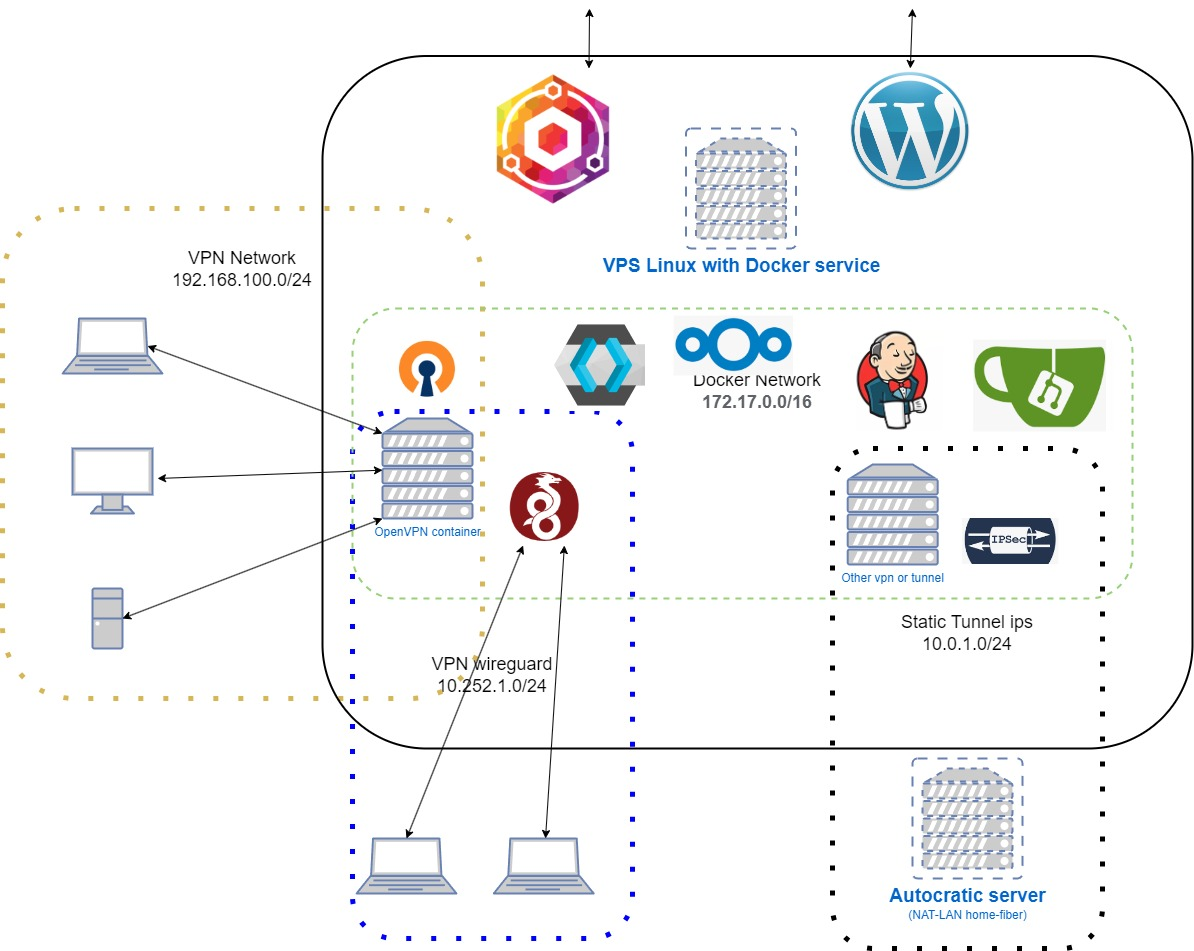
\includegraphics[width=0.9\textwidth]{./figuras/entorno_redes}
\caption{Casuística de interés de VPN - VPS.}
\label{F:entorno_redes}
\end{center}
\end{figure}

\begin{itemize}
    \item Túneles P2P, es decir, conexiones puntuales para interconectar redes o servidores. Usualmente estáticas, utilizadas como red de transporte troncal. Es una mono-red  ya que es un único enlace entre dos nodos y se les denomina como túneles ya que una vez entra el tráfico en ellas sale en el destino.
    \item VPN como servicio-salida a internet, aunque puede ser entendido como un nodo central de enlaces p2p, formando una red al re-enrutar tráfico en el nodo central, su objetivo radica como puerta de enlace para conectar clientes externos. Su objetivo principal es acceder a intranets y geo-localizar el cliente dentro de la intranet, saliendo al exterior con IP y legalidad del servidor VPS. 
    \item Conectar o exponer elementos de manera sencilla sin necesidad de IP pública, pre-configurado de nat-reverse y firewall. Se utiliza un cliente de una conexión reversa a una VPN como servicio-salida, evitando problemas intermedios tales como NAT, firewall, CG-NAT\cite{c_cg_nat} de la red proveedora de conectividad, el objetivo en este caso no es el enrutado sobre la vpn, sino lo contrario, la exposición de un servicio en la propia VPN a internet a través de IP pública del VPS que ofrece la VPN.
    \item Seguridad y compartimentación, la red así como las intranet son una capa más de seguridad por aislamiento al cifrar una comunicación y limitar el acceso a las comunicaciones e imponer una barrera de acceso a recursos únicamente ofrecidos dentro de la intranet.
\end{itemize}


\section{Casuísticas de interés}
Obviando la conexión directa de elementos públicos o privados (detrás de NAT), o la definición propia de VPN para usar dicha red en nuestros objetivos existen un conjunto de situaciones que se resuelven con una implementación por defecto de VPN.

\subsection{ Interconexión de redes privadas por VPN}
Este caso es de interés muy habitual, múltiples LANs, especialmente si son redes de oficinas regionales, desean estar interconectadas de manera privada, es decir equivalente a interconectadas por cable, para permitir acceder a los diferentes servicios o clientes de cada una de ellas.
\begin{figure}[!htb]
\begin{center}
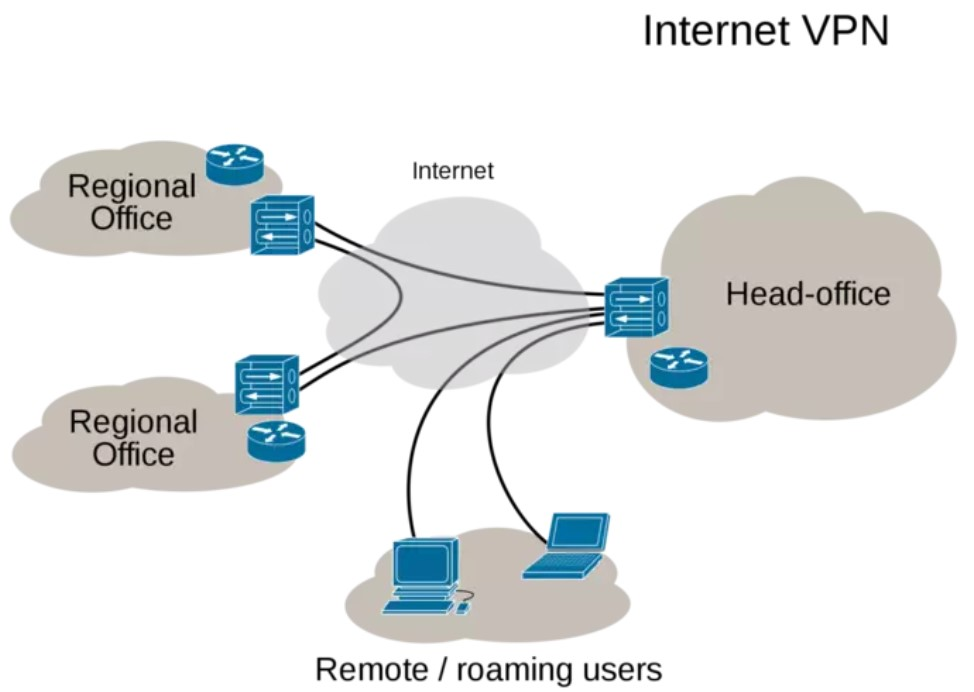
\includegraphics[width=0.75\textwidth]{./figuras/vpn_network_link}
\caption{Diagrama interconexión de redes por VPN\cite{i_redes_sedes}.}
\label{F:vpn_network_link}
\end{center}
\end{figure}
Se define una VPN, la cual actúa como red de transporte en forma de estrella, e incluye unas reglas de enrutado para anunciar y permitir la comunicación entra Lan - VPN- Lan. Véase anexo \ref{S:enrutado_sedes} con un caso detallado y explicado.

Los principales servicios más beneficiados son IT (soporte), servidores de almacenamiento en red y el uso de protocolos de comunicación (FTP, PING ..) entre elementos de ambas redes.

Un punto importante de la interconexión de LANs y VPS es el uso extensivo de captación de imágenes de seguridad y sensores tales como cámaras ip, sensores wifi o gateways de sensores (zigbee, z-wave o bluetooth) ya que son sistemas que suelen estar aislados a LANs no expuestas y no accesibles.

Se debe entender que no es necesario instalar un cliente VPN en cada elemento de la LAN, sino definir aquel elemento que “enruta” el tráfico por la vpn o utilizar un router con cliente VPN ( véase anexo \ref{S:enrutado_sedes}).

\subsection{ Múltiples capas de VPN}\label{S:doble_layer}
Desde la perspectiva de seguridad pero especialmente para la separación de conocimiento o grupos de trabajo existe la necesidad de una VPN principal (intranet) para acceder a los servicios esenciales y la conectividad una vez ya dentro de la intranet de otras VPN para redes concretas no expuestas por el VPS. Esto también aplica a la gestión UI de la propia VPN-layer2 evitando puntos de ataque por no estar expuesta a internet.

\begin{figure}[!htb]
\begin{center}
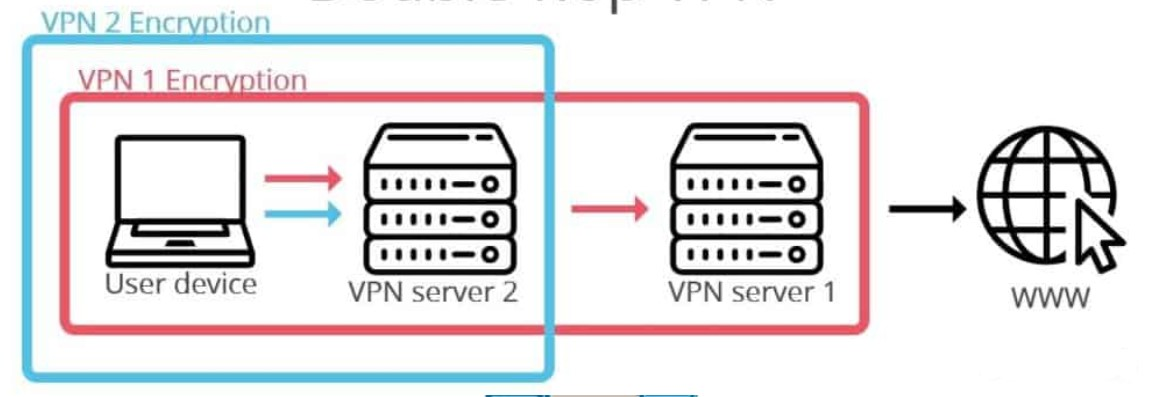
\includegraphics[width=0.75\textwidth]{./figuras/vpn_ultiples_layers}
\caption{VPN multi-salto, multi-capa.}
\label{F:vpn_ultiples_layers}
\end{center}
\end{figure}

De especial interés también puede ser el uso de una o mas tecnologías vpn, combinando diferentes capas y tecnologías.

\subsection{DNS filtro y espejos.}

Un servicio DSN-proxy interno es de especial necesidad para ofrecer una interfaz intuitiva al acceso de los servicios internos, así como filtro de seguridad capaz de filtrar publicidad o accesos web inseguras o en black list similares a pihole\cite{c_pi_hole}.
\begin{figure}[!htb]
\begin{center}
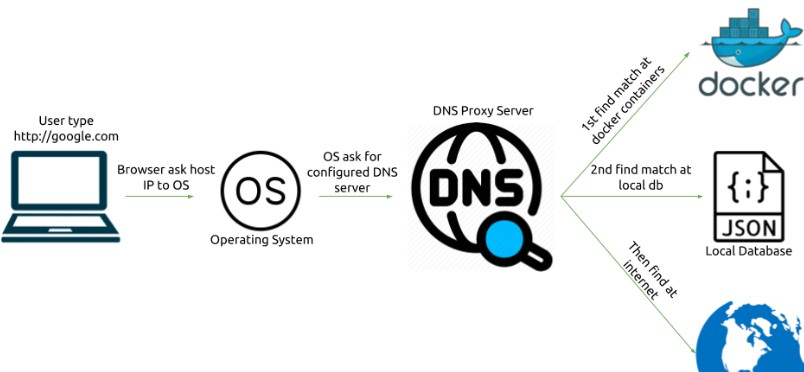
\includegraphics[width=0.8\textwidth]{./figuras/dns-proxy.jpg}
\caption{Diagrama DNS proxy\cite{i_dns}.}
\label{F:dns_proxy}
\end{center}
\end{figure}
Dentro de la VPN es de especial utilidad puesto que los servicios dockerizados no expuestos no tiene una IP estática, por consiguiente la asignación de un DNS interno que contenga los dominios internos dentro de la VPN es algo necesario (véase anexo \ref{S:dns}).

Finalmente existe la necesidad de creación de repositorios espejos, es decir, se bloquea el acceso a repositorios de uso común como dockerhub, maven, node etc.. y se crea un repositorio interno espejo que cachea o generan repositorios “aptos” (aprobados por seguridad o pendientes de auditar), para su uso interno como espejo de los públicos.

\subsection{Exposición externa vía VPS}
A veces no disponer de recursos, una ip pública en una sede o restricciones legales es un impedimento para ejecutar servicios en dicho lugar geográfico.
En estos casos se utiliza un elemento publico adecuado (IP y ubicación) para tunelar trafico (vía VPN) a nuestros recursos privados.
\begin{figure}[!htb]
\begin{center}
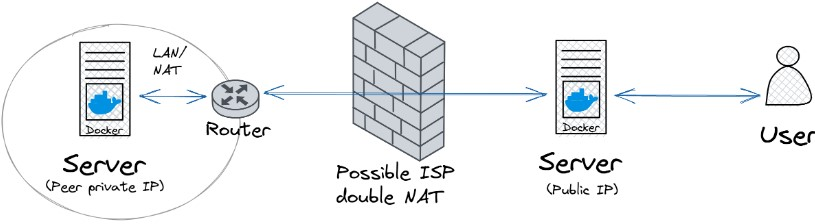
\includegraphics[width=1\textwidth]{./figuras/tunnel_resources.jpg}
\caption{Conexión a recursos detrás de CG-NAT / Firewall o NAT.}
\label{F:tunnel_resources}
\end{center}
\end{figure}

Por otra parte la exposición de los recursos detrás del tunel pueden ser expuestos utilizando una técnica de "proxy reverse", que es también utilizada como automatización de multi-dominio en el propio servidor VPS. Otro interés puede ser la atenuación de ataques o recopilación de estadísticas si nuestra nube de gran potencia pasa por proxy en un VPS, fácilmente bloqueable o parapetado con un firewall.

\begin{figure}[!htb]
\begin{center}
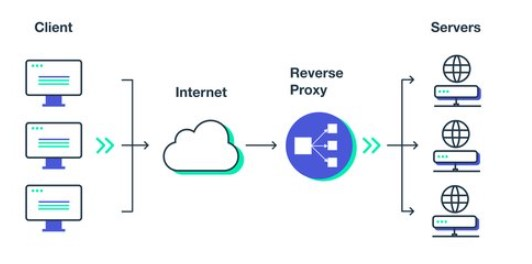
\includegraphics[width=0.8\textwidth]{./figuras/reverse_proxy.jpg}
\caption{Reverse proxy diagram.}
\label{F:reverse_proxy}
\end{center}
\end{figure}

 Un ejemplo simple es la reconversión de una vieja bodega en un pequeño cluster de servidores para un proveedor de pymes. Probablemente el aislamiento y temperatura de la bodega, es idóneo para la refrigeración y uso continuado de los servidores, así como la utilización de recursos verdes para generación eléctrica o refrigeración activa fácilmente amortizables. Sin embargo el coste de un enlace público o geo-localizar la ip del cluster puede tener costes elevados(económicos o de seguridad), mientras que la contratación de dos proveedores de fibra, debido a las altas capacidades actuales (300-1000 Mbps) permite un uso profesional de enlaces de público general.

\section{Docker y automatización de redes}

Docker permite crear diferentes tipos de redes virtuales e interconectar los contenedores docker a una o más de ellas.
Aquellos contenedores públicos, tiene los puertos directamente mapeado a la red hospedante del vps, sin embargo todos aquellos servicios no expuestos ( db, dns, servicios privados) para evitar la interconexión de todos por una red bridge default y su vulnerabilidad de seguridad, se definen diferentes redes por temática (auxiliar, wordpress, vpn-layer1, vpn-layer 2 ...).

Los contenedores que pertenecen a más de una red, se interconectan a ambas donde la red default gateway es la primera conectada en orden alfabético.

Así mismo recordemos que docker contiene un dns interno que es capaz de redirigir nombre del servicio, id, hostname, alias de red. Esta redirección depende del contexto, es decir, si dos contenedores están en redes diferentes aisladas, la resolución no devolverá ip alguna, en caso de haber conectividad redirigirá a la ip interna de la interfaz de conexión.

\subsection{Automatizaciones}
Con el fin de evitar la creación de configuraciones estáticas o complejas, se ha optado por un enfoque automático y auto generado, es decir, cada vez que desplegamos un contenedores en un red de docker aquellos servicios como proxies, dns, portainer y otros elementos monitorizadores deben conocer de la existencia de los nuevos contenedores y auto configurarse para su correcto funcionamiento.

Esto se consigue mediante Docker out of Docker\cite{c_dood} véase anexo \ref{S:docker_compose_details} y dockergen\cite{c_docker_gen}, estos mecanismos permite acceder desde los contenedores a meta-datos de otros contenedores en ejecución, especialmente variables, labels y propiedades de redes. 

\subsection{Reverse Proxy y HTTPS}
La primera automatización es el uso de un reverse proxy con certificados https automáticos, es decir, aquellos contenedores públicos se subscriben junto a un Traefik\cite{c_traefik} o Ngix\cite{c_ngix} proxy que gracias a un container de let's encrypt\cite{c_letsencrypt} y las utilidades de Dood\cite{c_dood} y dockergen\cite{c_docker_gen}, identifican los hostname, dominio o alias de los container, generan el certificado de let's encrypt y la configuración de reverse-proxy hacia los puertos indicados, véase flechas verdes figura \ref{F:entorno-dockerNetworks} o prueba de concepto anexo \ref{S:reverse_proxy_example}.

Por consiguiente únicamente con definir las variables y deployar en la red docker, el contenedor es accesible via el puerto 80/443 con https certificado públicamente hacia el dominio preseleccionado en las variables del contenedor (únicamente requiere tener registrado el dominio y la redirección pertinente hacia el VPS).

\subsection{Dns automatizado}
De una manera similar, puesto que docker internamente auto gestiona un dns propio, util, y actualizado es posible la utilización de dns proxy-relay, utilizando como master el dns interno de docker basado en Docker out of docker\cite{c_dood} o la extensión del contenedor con resolver basado en el dns docker.

Por lo tanto en base al dns master de docker, resolverá la petición en local (hosts files y resolv de VPS hospedante), después resolverá los valores entre los diferentes valores docker internos, se puede configurar un segundo nivel local en base de datos local del contenedor dns (json, db, dominios internos seteados por UI manualmente) y finalmente llamara a los dns externos que utiliza el VPS.

Es por lo tanto un sistema completo de dns en si puesto que permite todas las peticiones dentro de la red docker. Debido a que es posible situar el servicio de VPN en dicha red y utilizarla como default gateway, obtenemos un dns 100\% funcional para peticiones internas como externas, al utilizar el VPS como default gateway a internet (véase  figura \ref{F:entorno-dockerNetworks}).

\subsection{Interconexión de Red docker, VPN y gateway}

Existe un problema, para permitir la conectividad vía default gateway via VPS. No es posible salir a internet con IP internas de una VPN, es decir privadas. Es necesario la utilización de un mecanismo de NAT-Masquerade, para que sea la IP del VPS.

Este mecanismo esta proporcionado nativa mente en docker, por ello desde dentro de un container podemos acceder a internet, ya que entre las ip publica del VPS y las redes internas de Docker hay un NAT funcionando. Sin embargo desde la VPN únicamente esta habilitado el enrutado a otras redes, es decir, requiere de una NAT entre la red VPN y la red interna de docker que el servidor de VPN tiene como default gateway.

Por otra parte este NAT red VPN hacia las redes del contenedor-servidor VPN, puede tener especial utilidad, ya que las NAT se pueden definir por interfaces o dominios de redes. Esto nos permite hacer que toda petición proveniente de la VPN paredca estar originada en el propio VPN-server container, el cual si esta conectado a mas de una red (default gateway u otras), nos permita una comunicación  de la VPN hacia los servicios dockerizados. Esta comunicación es unidireccional, es decir debe ser preestablecida en ese orden para ser bidireccional, por lo que inhabilita la posibilidad de acceder desde los contenedores dockerizados a IPs concretas de la VPN.

Otro elemento interesante es la declaración de dominios internos que apuntan a ip's internas de la VPN para servicios entre sedes. Aunque dichas ips no son accesibles desde los servicios dockerizados en el VPS, si lo son desde la VPN, por lo que el servicio dns configurado manualmente es funcional para todo elemento conectado a la VPN.

Como conclusión, aquellos elementos conectados a la VPN, pueden:
\begin{itemize}
    \item Usar la VPN como default gateway, saliendo a internet por el VPS (flechas rojas, figura \ref{F:entorno-dockerNetworks}).
    \item Definir como servicio de dns, el contenedor dns-proxy interno, permitiendo resolver dominios internos y utilizando los dns externos apropiados para la ip del VPS.
    \item Conectarse y utilizar todos los servicios expuestos en las redes internas de docker a los que el contenedor servidor VPN esta conectado.
    \item Conectividad con las LANs de sedes, si estas son expuestas a través de la VPN si existe un elemento conectado a ambas (VPN y LAN) configurado como gateway LAN-VPN-LAN.
    \item Exposición remota de servicios, en aquellas VPN de mecanismos inverso (flecha negra figura \ref{F:entorno-dockerNetworks}).
\end{itemize}
\begin{figure}[!htb]
\begin{center}
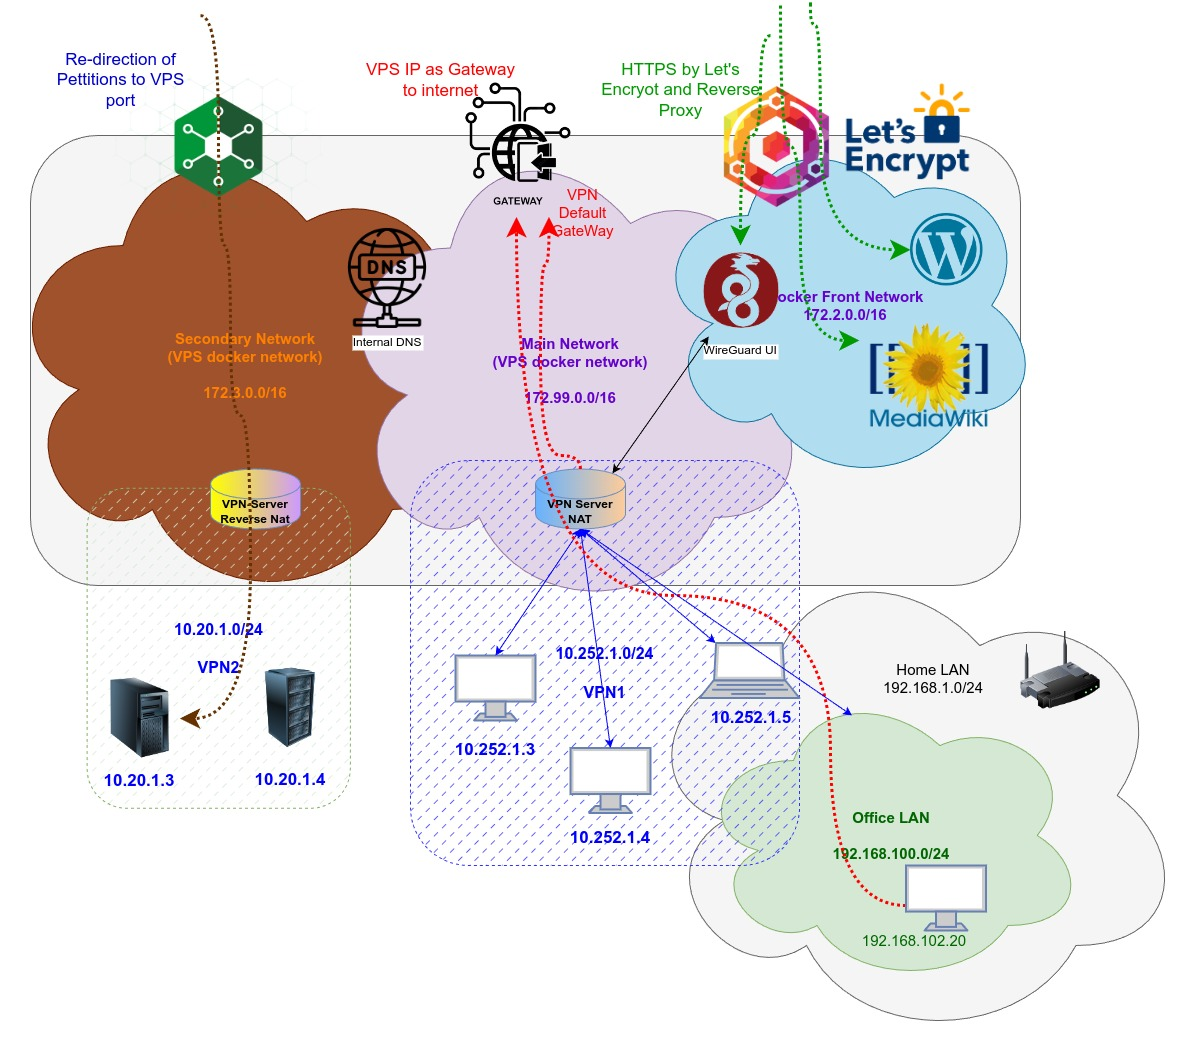
\includegraphics[width=1\textwidth]{./figuras/entorno-dockerNetworks.jpg}
\caption{Diagrama de interconexión de redes docker y servicios.}
\label{F:entorno-dockerNetworks}
\end{center}
\end{figure}
Por otra parte, si deseamos que nuestra VPN permita un acceso reverso, es decir enviar peticiones o trafico desde la red docker a nuestra IP en la VPN o nuestra LAN expuesta por dicha IP-vpn, no es posible la utilización de los servicios dockerizados, o el uso de la VPN como default gateway, ya que requiere implementar un Nat-reverso docker-network a VPN (véase flechas marrones figura \ref{F:entorno-dockerNetworks}),
o una configuración especifica (estática) de DMZ para permitir conexiones especificas a través del NAT.

Por ultimo para la interconexión de sedes, es indiferente, ya que las sedes pueden comunicarse a través de la red VPN, sin necesidad de pasar por las redes docker y no se ven afectadas por ningún tipo de NAT, únicamente es necesario tener un elemento conectado a la VPN en dichas LAN y la configuración adecuada.

\section{Caso desarrollado}
El caso desarrollado se ha centrado en la implementación de 3 VPN, focalizados en tres objetivos diferenciados (véase figura \ref{F:red_entorno_vpn}). 

Una primera VPN1 cuyo objetivo es la interconexión de elementos de la VPN(principal), la salida como puerta de enlace por el VPS y el acceso a servicios dockerizados internos (DNS, web, internos …). Una segunda VPN2 cuyo principal objetivo es la interconexión de LANs o enrutado. Y por último una tercera VPN3 que se puede acceder únicamente conectado a la VPN1 / VPN2, es decir una segunda capa VPN como explica el punto \ref{S:doble_layer} para aquellos servicios seguros y no disponibles desde la red principal del cloud.

\begin{figure}[!htb]
\begin{center}
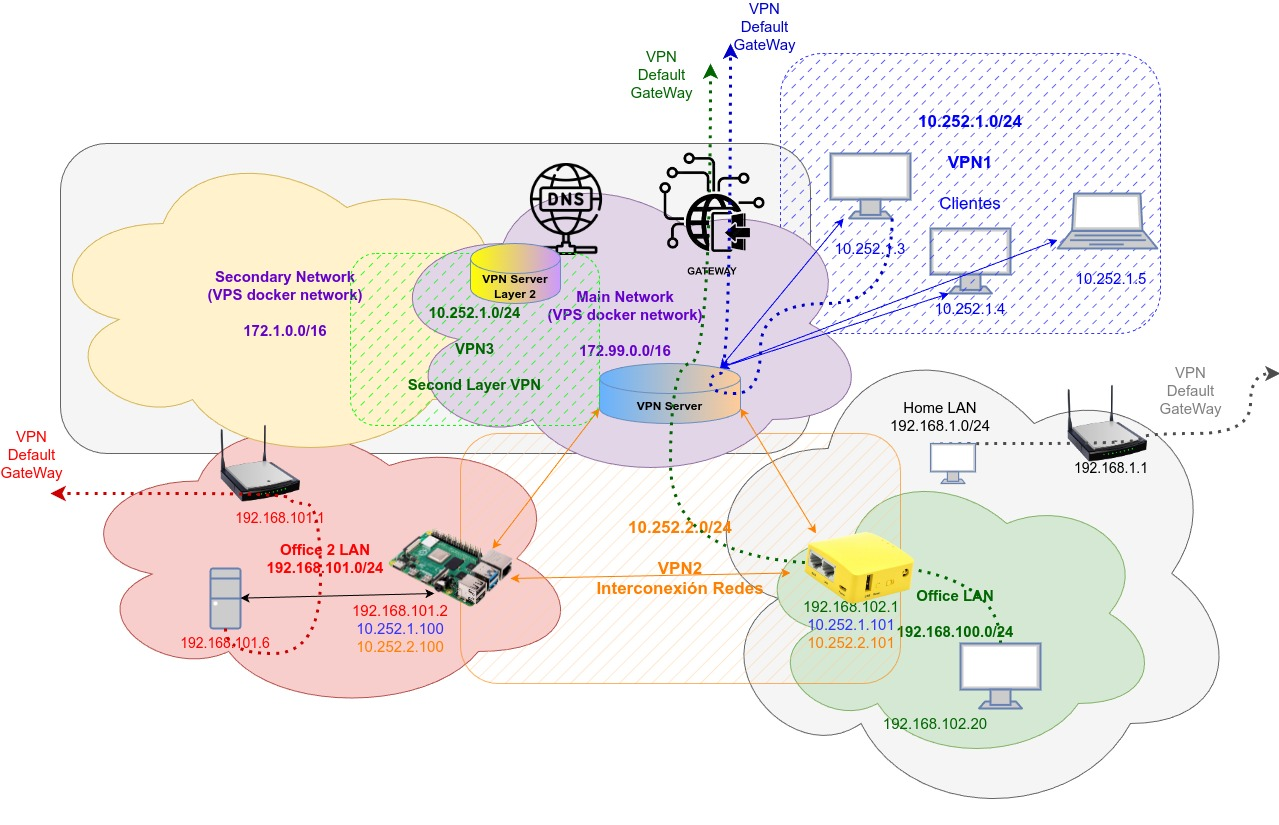
\includegraphics[width=1\textwidth]{./figuras/red_entorno_vpn}
\caption{VPNs, relación entre ellas VPS y clientes.}
\label{F:red_entorno_vpn}
\end{center}
\end{figure}

En el diagrama de la figura \ref{F:red_entorno_vpn} se muestra un ejemplo real donde tenemos 8 redes diferentes, 3 LAN, 3 VPN, y 2 redes docker:
\begin{itemize}
    \item VPN1 10.252.1.0/24 (azul) , cuyos clientes entunelan tráfico en esta red virtual privada, gestionada por el VPN server. Implementa un NAT masquerade de azul-morado, provee de acceso a internet y conectividad con los servicios dockerizdos de la red morada.
    \item VPN2 10.252.2.0/24 (naranja) , cuyos clientes entunelan tráfico en esta red virtual privada, gestionada por el VPN server. Provee conectividad de la red docker hacia las LAN de sedes y viceversa.
    \item Docker network 172.99.0.0/16 (morada), es una red privada de docker donde están la mayoría de  servicios docker del VPS. Permite enrutar tráfico a través del VPS al exterior. Las sedes tiene conectividad con dichos servicios vía VPN2 así como el resto de clientes de VPN1. Es la red principal del cloud-VPS.
    \item Office 2 LAN, 192.168.101.0/24 (rojo) compuesta por una oficina con router ADSL/fibra en la cual existe un dispositivo raspberry pi conectado a la VPN2. Permite acceder a la red morada (docker con servicios) y otras sedes (LAN verde oscuro). Ejemplo de casuística con default gateway por su propio router, no es por el VPS.
    \item Office LAN, 192.168.100.0/24 (verde oscuro) compuesta por una sede en casa con su propia LAN 192.168.1.0/24 adsl/fibra (gris) en la que se ha instalado un router wifi que habilita un NAT entre ambas e implementa un cliente vpn directo a la VPN2. Básicamente usa la red gris como infraestructura, se conecta vía VPN2 para enrutar todo el tráfico VPN-Red Docker hasta salir por el gateway del VPS. 
    \item  HomeLAN 192.168.1.0/24 (gris), LAN local de soporte a una red de oficina. Se puede observar como la red gris es independiente, no puede acceder a la red verde, ni ninguna otra red y su default gateway es su router, únicamente es usada como infraestructura.
    \item VPN Layer 2, VPN3 10.252.1.0/24 (verde claro), es una VPN únicamente accesible desde la red morada, es decir, se requiere de la VPN1 o estar en alguna LAN conectada a la VPN2 para poder acceder a ella. Similar a la VPN1-morada, realiza una conexión VPN3-amarilla, permitiendo acceder aquellos servicios dockerizados en la red docker interna amarilla y proveyendo de default gateway vía la red amarilla de docker.
    \item Second Docker net, 172.1.0.0/16 (amarilla) es otra red interna de docker la cual solo se puede acceder vía VPN3 que a su ves solo es accesible vía VPN1/VPN2. Es un caso de doble capa de VPN para acceder a los servicios.
    
    \item Elementos conectados a la VPN1, red azul, desde otros accesos, son terminales tunelados, es decir, su default gateway pasa a ser el VPS y usan el dns interno de la red morada docker. Tienen completa conectividad con los servicios de la red morada.
\end{itemize}

\section{Generalización de Casos}
Con el fin de explicar todas las posibilidades que brinda la nube generada en este documento, explicaremos los diferentes casos de uso general generar a través del diagrama de red de la figura \ref{F:red_entorno_vpn} y de la figura \ref{F:entorno-dockerNetworks} :
\begin{itemize}
    \item[--] Red verde oscura, es un ejemplo de despliegue por router portable, permite llegar a cualquier lugar y conectar por cable dicho router que genera un LAN autoconfigurada vía VPN2 a los servicios principales del VPS.
    \item[--] Red roja, es un ejemplo de sede conectada al VPS. No modifica la funcionalidad de la red, pero añade rutas estáticas de enrutado a través de un elemento conectado a la VPN2 en este caso una raspberry pi.
    \item[--] Red azul, es un ejemplo de VPN clásica, provee de acceso a internet vía VPS y permite la inter conectividad a diferentes redes (intranet). Aunque los clientes pertenecientes a dicha red (VPN1) pueden verse entre si, pero no son accesibles directamente desde el VPS ni exponen sus propias LAN.
    \item[--] Red naranja, en el diagrama \ref{F:red_entorno_vpn} es usada como infraestructura de interconexión entre sedes. Sin embargo puede ser utilizada como una VPN parcial similar a VPN1 pero sin usar el VPS como default gateway o utilizando los dns internos como alternativos, únicamente se utiliza para acceder a unos servicios concretos, especialmente si están en otras sedes.
    \item[--] Red morada, es una red virtual dentro del contexto del VPS. Es la \textbf{RED PRINCIPAL} de nuestro cloud, es decir la red troncal y en ella se sitúan los servicios dockerizados, está conectada a nivel bridge con el VPS por lo actúa como VPS-gateway y  como proveedor de dns internos. Aunque la gran mayoría de servicios son internos, un mínimo de ellos es publico (vpn server) o compartidos con otras redes docker.
    \item[--] Red verde clara, es un claro ejemplo de VPN múltiple layer, genera una VPN3 que solo es accesible una vez conectado a la VPN1 o VPN2.
     \item[--] Red amarilla, es un  caso de red aislada de docker, no accesible desde el exterior, requiere de una o mas VPN para ser accesible. 
    \item[--] Red gris, ejemplo de red de infraestructura sin acceso o interacción con las redes de cloud-VPS.
    \item[--] Red marrón, figura \ref{F:entorno-dockerNetworks} ejemplo de red docker interna con proxy de redirección, es decir, puede contener ciertos servicios expuestos, pero su principal función es exponer clientes VPN a través de un Nat-reverse y un reverse-Proxy en la ip del VPS.
    \item[--] Red azul claso, figura \ref{F:entorno-dockerNetworks} ejemplo de red docker con servicios públicos con su principal característica es un reverse-Proxy y let's encrypt para generar HTTPS en los servicios expuestos. Es una red aislada de la red principal (morada), aunque varios servicios puede estar en ambas redes como por ejemplo la front-ui de el servidor VPN.
\end{itemize}

\chapter{Desarrollo de software}\label{S:tema_4}
Para el desarrollo de software de una manera adecuada, profesional e interdisciplinar (independiente de lenguaje, framework o grupo de trabajo) es necesario no solo unas herramientas en común, sino unas dinámicas de trabajo en equipo y especialmente una metodología de trabajo técnica, profesionalizada.

Usualmente se entiende que aunque un autónomo o freelance desarrollan un trabajo adecuado, en software el review o validación por terceros es un elemento crítico en la filosofía de verificación mejora y calidad del producto por ello asumimos que el entorno de trabajo cuenta siempre con un mínimo de 3-4 personas que forma un equipo técnico.

Por otra parte el equipo asume que tanto las tareas a realizar como la responsabilidad de las mismas no es personal sino grupal, por lo que todo el equipo debe ser involucrado en las tareas de gestión, desarrollo, testeo, documentación y puesta en marcha de la aplicación.

\section{Dinámica de trabajo (equipo)}
Actualmente por contexto laboral, las filosofía de trabajo AGILE\cite{c_agile}, y en concreto SCRUM\cite{c_scrum} son de amplia aceptación y exitosas. Por ello son las seleccionadas por este documento.

\subsection{Agile}
Agile es una metodología de trabajo cuya principal enfoque reside en la gestión de equipos y proyectos; define la manera de interaccionar personas, herramientas y procesos favoreciendo la colaboración con el cliente por encima de la negociación contractual. Su principal objetivo es el desarrollo de software funcional y la flexibilidad o respuesta al cambio a la hora de seguir una planificación.

\begin{figure}[!htb]
\begin{center}
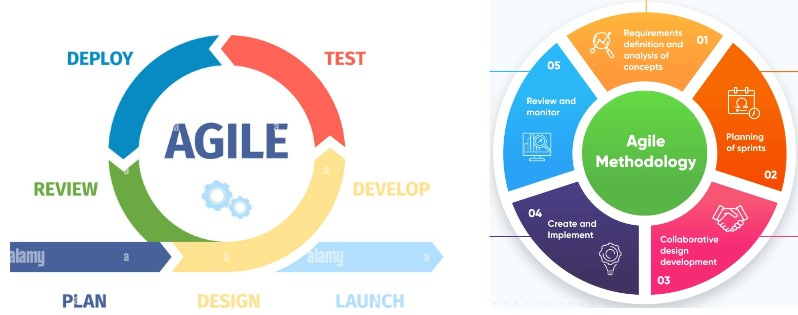
\includegraphics[width=1\textwidth]{./figuras/agile}
\caption{Diagrama metodología AGILE.}
\label{F:agile}
\end{center}
\end{figure}

\subsection{Scrum}
Scrum es la implementación de una filosofía agile, destaca por su aproximación en fases y división del tiempo de trabajo en sprints (2-3 semanas de trabajo). El objetivo de scrum es la mejora continua, facilitando el valor añadido en un calendario de entregas, para ello define unas fases de planificación, evaluaciones diarias, re-definición, review y retrospectiva. Existen roles como el product owner que interacciona con los clientes para garantizar que se entienden los requisitos y se alcanzan los objetivos marcados para cada sprint. El equipo utiliza las “historias” del cliente-product owner, para definir tareas funcionales, estas deben ser especificadas y estimada por el equipo dentro de un backlog.

\begin{figure}[!htb]
\begin{center}
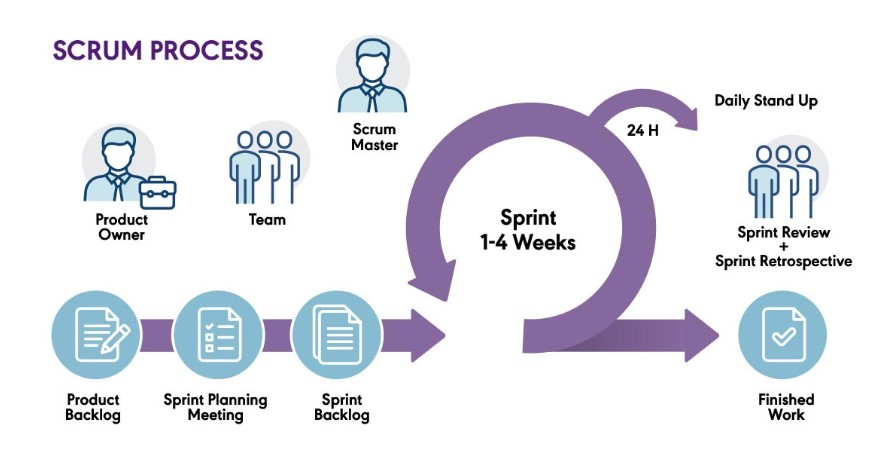
\includegraphics[width=1\textwidth]{./figuras/scrum}
\caption{Diagrama funcionamiento SCRUM-AGILE\cite{i_scrum}.}
\label{F:scrum}
\end{center}
\end{figure}
El scrum master es el encargado de facilitar y supervisar el funcionamiento del scrum, dirigiendo las reuniones. El y el equipo planifican los tickets a realizar en un sprint, entre los estimados del backlog. Diariamente se comenta brevemente el trabajo realizado, problemas abordados del día anterior y la previsión diaria.

En caso de cambios no planificados se re-priorizan los tickets y se redefine el sprint restante, con el fin de obtener siempre una mayor satisfacción en la entrega. Una vez acabado el sprint, se realiza un proceso de review con el cliente con feedback real y de calidad sobre el resultado obtenido así como una retrospectiva del equipo sobre que se hizo bien, mal, causas, mejoras a implementar especialmente desde el punto de vista de gestión e información dentro del equipo.

Desde el puntos de vista técnico, cada cambio no solo está traceado por un ticket del sprint, sino que debe incluir las siguiente apartados:
\begin{itemize}
    \item Documentación, descripción técnica de los cambios realizados por la tarea, que fundamenta la documentación general del software.
    \item Pull request, con el código de la tarea, auto-explicativo o apropiadamente documentado. Todo código debe respetar un código de buenas prácticas general o definido por el equipo. Test unitario o de integración que validan la funcionalidad añadida.
    \item Validación de un CI build con revisión aprobada, donde se compila ejecuta los test, se pasa validadores de calidad de código o vulnerabilidades como sonar\cite{c_sonar} o blackduck\cite{c_blackduck}. Review cualitativo de otros programadores y review en profundidad por aquellos que conocen la naturaleza del servicio o los cambios (approved).
\end{itemize}

\subsection{Generalización y profesionalidad}
La importancia tanto de la metodología de equipo, como las buenas prácticas y estructuras de trabajo no solo aporta robustez, calidad y estandarización al trabajo entregado, sino que permite optimizar al equipo como cadena de trabajo.

 Un caso destacado del trabajo estandarizado es la generalización de tareas, es decir, cualquier elemento del equipo puede asumir o traspasar tareas aunque no sean suyas, ya que el código debe ser fácilmente legible, testeado y documentado; fielmente protocolizado. Y este punto normalmente es inviable en equipos inferiores a 3-4 personas, donde no hay una dinámica de trabajo en equipo, sino división del trabajo y asignación de elementos.

Por ello la transferencia de tareas/código tienden a generar refactorizaciones o recreaciones de software ante la inviabilidad de mantenimiento o comprensión por ser un software no estandarizado o dicho de otra forma, creado por desarrolladores que no saben trabajar en equipo, o no profesionalizan su trabajo ya que no puede ser transferido.

\section{Git, CI/CD y contenedor}
Actualmente toda empresa de software debe de tener un control sobre los cambios del software y mecanismos automatizados para la evaluación del mismo. Pasar código por mail, usb o un almacenamiento en la nube no solo es un riesgo de seguridad sino que no es profesional y es el principio de un ciclo de malas praxis.

\subsection{Git y repositorios de código}
Git\cite{c_git} es un programa de control de versión, significa que define versiones de código, permite generar nuevas versiones cuando se le generan cambios al código. 

Permite calcular las diferencias entre versiones del código anterior y realizar “commits”, es decir, aglutinar un conjunto de cambios y almacenarlos como diferencias entre la versión anterior y nueva. Este commit, incluye un mensaje descriptivo de los cambios y en muchas ocasiones código o nombres del ticket asociado para trazabilizar el cambio.

El código se construye desde un commit inicial a la versión deseada, esta aplicación de las diferencias, permite la generación de “ramas” en base a aplicar unos cambios u otros. 

El concepto de rama permite establecer versiones en paralelo del mismo software, así mismo permite unir ramas (merge) o crear nuevas a partir de las anteriores.
\begin{figure}[!htb]
\begin{center}
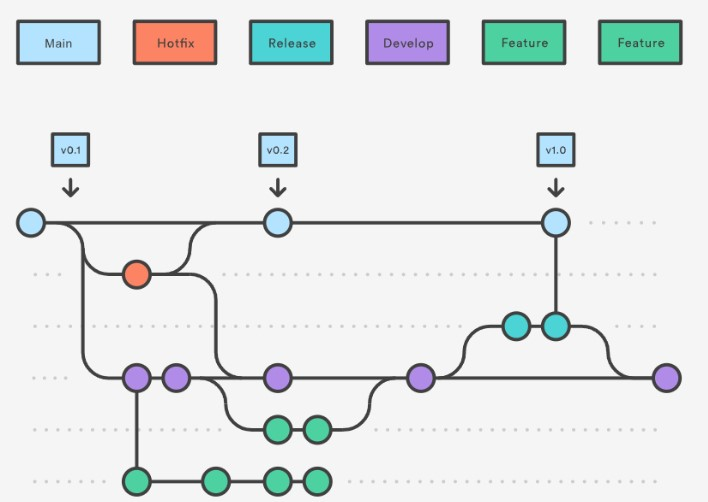
\includegraphics[width=1\textwidth]{./figuras/git_flow}
\caption{Diagrama flujo de trabajo en git\cite{i_git_flow}.}
\label{F:git_flow}
\end{center}
\end{figure}
 El verdadero potencial de este software es un repositorio o servidor git en línea, el concepto es sincronizar nuestro git local con repositorios en remoto que también sincronizan con otros desarrolladores de software. 
 
 Establecida una dinámica de trabajo (git flow figura \ref{F:git_flow}), permite trabajar de manera paralela a programadores sobre el mismo código sin “pisarse” y sobre todo, tracear y poder volver a versiones anteriores del código, sean nuestras o de otros desarrolladores.
 
\subsection{CI/CD}
CI/CD se refiere a las siglas de Integración Continua / Entrega Continua en inglés, es un concepto que se basa en el uso del repositorio de git y un código apropiadamente testeado.

Cuando se termina una tarea, el desarrollador realiza un PR (Pull Request) que inicia una petición de revisión de los commits añadidos para la funcionalidad, esta petición acciona un programa agente, que compila y ejecuta los test. Si es satisfactorio almacena la nueva versión del código compilado en un repositorio no de código sino de binarios/paquetes (según sea el lenguaje utilizado) y espera el 'ok' de otros programadores en el PR. Esta acción de construcción y testeo continuada de versiones del software o integración (CI), puede ser acompañada de script automatizados que despliegan (CD) directamente el software construido en una plataforma de trabajo, que puede ser desarrollo, test o directamente producción, es decir, continuamente se entregan versiones nuevas del software.

Como último eslabón, tenemos la 'contenerización' que en nuestro caso de uso es dockerizacion, es decir, generar un contenedor docker con los binarios generados por el CI y guardar la imagen en un repositorio de contenedores, para que el CD únicamente tenga que actualizar la imagen docker vieja por una versión más nueva en nuestro orquestador de despliegue.

\subsection{Opinión de un usuario con experiencia}
La combinación de un equipo agile con un entorno de git + CI/CD, más el uso de contenedores, permite el desarrollo en paralelo y revisión de tareas fácilmente, donde en cada cambio se valida el software y construye una nueva imagen, se despliega automáticamente sin riesgo humano. Todo ello con los beneficios intrínsecos mencionados que aporta docker a un software.

En mi opinión, este proceso completo únicamente se da en grandes empresas o startups tecnológicas con personal cualificado, pero en más del 50 \% de las pymes relacionadas con software o pequeños departamentos de software de grandes empresas, falla estrepitosamente, es decir, o no se aplica al completo o no se quieren aplicar tanto las metodologías de equipo o las automatizaciones y requisitos técnicos.

\section{CI basado en docker}
Históricamente se ha evolucionado desde un CI/CD de binarios, hacia un CI de binarios, que se construyen en un contenedor y el CD usa directamente el contenedor.

 El caso más utilizado jenkins\cite{c_jenkins}, es un agente multi-plugin que permite prácticamente la ejecución de cualquier lenguaje de programación, orquestador de dependencias y el uso  de terceras aplicaciones. El problema reside en que el agente debe tener acceso a máquinas con el compilador, máquina virtual o dependencias necesarias para la compilación y ejecución de los test. Al igual que un servidor linux, requiere de un mantenimiento y complejidad a la hora de gestionar adecuadamente las versiones y compiladores; especialmente cuando una empresa cuenta con múltiples equipos donde cada uno con un producto que puede tener requisitos diferentes.

 Una primera solución es el uso de docker como “aplicación”, es decir, utilizar los binarios de un container para ejecutar comandos específicos utilizando el directorio de trabajo como volumen. Así, una ejecución de maven/gcc/node/composer para generar los binarios/archivos necesarios y/o permite ejecutar los test. En dicho caso se reduce el mantenimiento, pero requiere de múltiples imágenes docker en el agente-ci.

En nuestro caso de interés, no disponemos de servidores-agentes sino que nuestra intención es que un container docker ejerza de agente-ci y por definición un container debe ser ligero. El punto novedoso, es el uso de container, con docker instalado, es decir, Docker in docker\cite{c_dind} y build ci\cite{c_ci_docker} en dockerfile con múltiples\cite{c_docker_multistage} etapas. Véase anexo \ref{S:docker_complex} docker desde dentro del propio contenedor. 

El segundo elemento es el uso de construcción de contenedores como build, es decir, compilar, ejecutar los test y construir la imagen en un único paso. Para ello se usa el concepto de múltiples etapas\cite{c_docker_multistage} que permite ejecutar pasos previos en imágenes base diferente que no son usadas para la imagen base final sino para la ejecución de comandos intermedios. 

Finalmente obtenemos que con solo docker instalado y la apropiada configuración, aquellos requisitos técnicos serán descargados como imágenes auxiliares usadas, y generan una imagen docker ligera únicamente con los ficheros necesario para la ejecución en producción.

\section{CI/CD dentro de nuestra nube}
Durante la realización de este documento se han realizado múltiples pruebas de concepto, entre ellas las prueba de un CI/CD basado en gitea\cite{c_gitea}-drone\cite{c_drone}. Al evaluar lo junto a servicios públicos externalizados como github\cite{c_github}, bitbucket\cite{c_bitbucket} o gitlab\cite{c_gitlab} entendemos que para un grupo reducido de desarrolladores es mas práctico y evita tareas de mantenimiento y segurización el uso de herramientas gratuitas externas. Sin embargo en aquellos casos donde el grupo de trabajo sea mas extenso o la naturaleza del código a generar tenga un carácter confidencial, se puede utilizar las pruebas conceptuales (véase anexo \ref{S:ci_ejemplo}) como parte de nuestra nube privada.

\section{Setup Software Local}
En los entornos locales puede haber una mayor diversidad de SO, ya que no es un elemento crítico para el desarrollo. Sin embargo debe existir una automatización y especialmente una estandarización con el objetivo de minimizar problemas o la no reproducción de circunstancias a la hora de depurar o corregir un error detectado en producción, por lo tanto es de especial interés que las versiones y software esté alineado no solo en producción sino entre los propios programadores (herramientas auxiliares). En los siguientes apartados se detallan las estrategias principales utilizadas como software-local para cliente de nuestra nube o herramientas y configuraciones de desarrollo.

\subsection{Automatización Local}
Podemos usar Scripting, principalmente bash o batch, aunque se recomienda el uso de ansible apuntado a localhost. Podemos distinguir varias tareas:
\begin{itemize}
    \item Instalación y configuraciones de elementos críticos de la compañía tales como cliente vpn, software de comunicaciones, correo o agentes de IT.
    \item Instalación de software necesario. Git, un gestor de repositorios git visual, compiladores, máquinas virtuales, IDE (Entornos de desarrollo), docker.
    \item Configuración de herramientas, gitignore, estandarización de IDE, puede ser definidas por la compañía, el grupo de trabajo o simplemente personalización individuales como los alias, guardadas en un repositorio de dot files.
\end{itemize}

\subsection{Herramientas de desarrollo basadas en docker}
Docker como compañía y empresa esta potenciando últimamente el segmento 'escritorio', especialmente en windows. Aunque docker CE (community edition) es open source, existe una versión privada con tools, interfaz gráfica y extras, dicha versión tiene engine para servidores y engine utilizada habitualmente en escritorio windows.

De una manera muy similar a la "dockerización de servicios", su intención es la dockerización de todo tipo de aplicaciones, especialmente UI, permitiendo instalar y gestionar programas en escritorio. Este nuevo enfoque facilita especialmente la automatización de herramientas necesarias en nuestro Sistema Operativo de escritorio, ya que uno de los problemas mayores es olvidar o seguir fielmente pasos de una guía de herramientas, así como la gestión de herramientas con diferentes versiones dependiendo de la fecha de aplicación de la guía.

Por otra parte, si por ejemplo trabajamos con diferentes versiones o dependencias, facilita mucho la instalación en paralelo de las mismas ya que todo queda dentro de un container. Un ejemplo puede ser un Docker-compose que integra las diferentes versiones de Java / pyhton/ php ..., el IDE de desarrollo, git y otras herramientas. Al igual que en el servidor únicamente con gestionar apropiadamente los volúmenes obtenernos un entorno funcional en segundos, con versiones estáticas y mas fáciles de actualizar.

\subsection{Dot files y configuraciones portables}
Recientemente se ha estandarizado una estrategia de archivos de configuración muy típica en el mundo linux/mac denominada “dot files”\cite{c_dot}\cite{c_dot_tools}. En los sistemas unix o derivados tiene archivos de configuración que normalmente usan el prefijo ‘.’ que a su vez indica un archivo oculto en el sistema. 

La gran mayoría son configuraciones default o de respaldo, ya que muchos software de desarrollo no solo deben estar apropiadamente configurados sino que existe una tendencia a configurar customizaciones, especialmente para la realización de atajos, alias o la configuración de múltiples softwares interaccionando o selecciones de versión default en caso de varias instalaciones.

En muchos casos no solo se trata de un trabajo detallado y costoso sino tuneado a lo largo de meses de pruebas, ensayos y errores. Además dichos ficheros suelen residir en carpetas especiales del usuario, carpeta de instalación o en directorios del sistema, añadiendo no solo una compleja trazabilidad sino la dependencia del lugar de instalación personalizado.

La estrategia de “dot files” se basa en la premisa de centralizar todos estos ficheros junto a scripts, alias y claves de una manera centralizada. Para ello en vez de editar los archivos originales se crean enlaces simbólicos de la carpeta centralizada a la posición de los archivos. Aquellos ficheros como claves o configuraciones sensibles son apropiadamente cifrados y se genera un inventario de “software dot file”, con el fin de automatizar su instalación, creación de links o la conmutación de configuraciones basada en perfiles. Finalmente esta carpeta está bajo control de versiones apropiadamente sincronizado con un repositorio(véase ejemplo de codelitv\cite{c_dot_repository}).

Como resultado se obtiene un control centralizado y sencillo de todas las configuraciones, un backup y restauración rápidos. Pero lo más importante un formateo-instalación o traspaso de configuración de SO rápido y eficiente, no estático, sino de manera continua ya que mediante git, se sincronizan diferente perfiles (ramas) de dot files en diferentes ordenadores, actualizando diariamente los cambios introducidos en otro pc.

\cleardoublepage
\phantomsection
\chapter{Conclusiones}
En la entrega de este documento (Octubre de 2023), se puede afirmar que la gran mayoría de los objetivos iniciales de este trabajo se han conseguido.

En primer lugar se ha planificado y ejecutado la creación de un lugar de teletrabajo adecuado para el autor, un trabajo continuo no exento de errores y mejoras realizadas durante el verano. Destacando especialmente en las comparativas con otros setup anteriores (anexo \ref{S:circunstancias}) y las soluciones aplicadas convergentes  con otros autores en temáticas similares \cite{c_overemployed}.

Segundo, se ha obtenido una nube virtual, económica, escalable fácilmente transferible que facilita y permite el teletrabajo. Especialmente aplicada a Elenkar S.L en el caso de mi pareja, pero de gran utilidad para proyectos personales o 'caseros'.

Por ultimo durante la investigación y recopilación se han comparado gran cantidad de servicios, tecnologías y proyectos basados en comunidades (véase tabla \ref{T:servicios_dockerizados} así como pruebas de concepto \ref{S:pruebas_concepto}), permitiendo seleccionar aquellos elementos mas útiles, ágiles y simples, que permiten ofrecer un producto customizable basado en un conglomerado de servicios gratuitos, LTS soportado por comunidades. 

Desde el punto de vista técnico la conjunción de servicios gestionado por docker, docker-compose y ansible, ha permitido un ágil despliegue, backup y restauración, minimizando el mantenimiento (véase \ref{lst:systemD_docker_reload}) o el conocimiento necesario para utilizarlo, mientras requiere de un perfil bajo de recursos de gran utilidad en pequeñas y medianas empresas.

En definitiva un boceto de producto comercial al por menor, que ya es explotado minoritaria-mente como pack de servicios similares externalizados\cite{c_tomahost}, productos especializados en casuísticas especificas como VPN\cite{c_procustodibus}, comunicación, web, almacenamientos(proveídos mismamente por VPS ovh\cite{c_vps_ovh}) o en autocracia (basada en raspberry pi) son por ejemplo Syncloud\cite{c_syncloud}.

En conclusión, este trabajo no solo muestra el conocimiento o un resumen del estado actual entorno al teletrabajo y las herramientas necesarias para implementarlo. Sino que existe un verdadero mercado segmentado en la puesta en marcha de los servicios o la gestión directa de ellos. En ambos casos son pequeñas y mediana empresas, sin recursos donde normalmente uno de sus proveedores de red / material / hosting / vps / proveedore de software (web) han aceptado un rol de montaje, gestión y mantenimiento como una segunda fuente de ingresos pero especialmente como servicio \textbf{diferenciador} y complementario a sus clientes.

\section{Conclusiones de la aplicación en Elenkar}
Elenkar S.L es una pequeña empresa de 3-4 trabajadores enfocada en servicios inmobiliarios y servicios exclusivos relacionados, afincada en el baix penedes.

Sus principales necesidades son Web (captación de clientes), mail (método de comunicación vía internet), capacidad de almacenaje y compartición de documentos (dropbox / drive) con otras inmobiliarias/clientes.

Tras la aplicación de este documento se ha conseguido:
\begin{itemize}
    \item Planificación real, y mejora de los recursos hardware, como software externalizados bajo el mismo presupuesto.
    \item Segurización y robusted real, tanto de red interna, interacción con clientes y vulnerabilidades de la gestión humana.
    \item Despliegue de recursos autócratas o confederales, a un coste low cost, que permiten reducir un presupuesto de 250€/anuales para un único servicio (dropbox), en un coste real de 60€/año por múltiples servicios incluyendo el almacenamiento en la nube.
    \item Acceso a servicios que han permitido la realización de trabajo en remoto parcial, VPN, acceso remoto, gestión centralizada de contraseñas seguras, control remoto de PC y compartición de recursos en remoto como impresoras, escáneres y servicios en red.
    \item El acceso a servicios no requeridos pero que mejoran el día a día como interacción de sensores y actuadores, gestión de alarmas o seguridad.
\end{itemize}

\section{Conclusiones Personales}
Desde el punto de vista personal puedo concluir que me ha permitido centralizar la casa de mis padres, casa de mi suegra, mi casa, otros inmuebles de una manera equivalente a las diversas sedes de una empresa. Y por similitud un soporte más directo y automatizado al no depender de terceras herramientas o de acciones humanas para configurar, arreglar elementos digitales.

Por otra parte como ayuda personal a proyecto de amigos/ex-compañeros, creo que les ha permitido reducir sus gastos iniciales así como reducir sus dependencias de softwares específicos, siendo una curva de aprendizaje más ligera para personas no técnicas, cuando se intenta realizar un proyecto personal de negocio.

\section{Trabajo futuro}
Aunque se ha obtenido el trabajo deseado y se han probado diversos conceptos de gran interés, se han detectado trabajos o conglomerados similares a este trabajo, especialmente focalizados en rasberry pi o en self hosting de servicios. Sin embargo todos ellos existen bajo un pretexto especializado o un conglomerado de servicios en pack, creo que lo que aun no existe en ningún producto privativo o opensource es el seleccionando de los casos de interés que autogenera la versión de docker-compose interesada o el despliegue directo de dicha versión sobre un VPS. Por lo tanto con posterioridad a este TFG, continuare con el provecto en vías personales para la extensión y automatización del mismo incluyendo una UI que lo haga aun mas asequible sin conocimiento técnico.


%%%  BIBLIOGRAFIA
%%%%%%%%%%%%%%%%%%%%%%%%%%%%%%%%%%%%%%%%%%%%%%%%%%%%%%%%%%%%%%%%%%%%%%%%%%

%%% Per la bibliografia hi ha 2 opcions: generarla amb la utilitat BibTeX 
%%%                                      o fer-la ''a ma''
%%% NOTA: podeu trobar facilment informació sobre BibTeX a:
%%%  http://www.ctan.org/tex-archive/biblio/bibtex/contrib/doc/

%%% OPCIO 1: BibTeX (recomanat) -> descomentar les comandes seguents:
%\bibliographystyle{unsrt}   %% Estil de bibliografia EETAC
%\cleardoublepage
%\phantomsection
% Indicar aqui el(s) fitxer(s) que contenen la bibliografia
%\bibliography{citacion-01.bib}  
%\pdfbookmark{Bibliografia}{sec:biblio}

%%% OPCIO 2: bibliografia manual
%%%
%%% L'argument d'entrada es el numero de referencies que s'inclouen
\cleardoublepage
\phantomsection
\begin{thebibliography}{2}

%% Llibres:  Autor/s (cognoms i inicials dels noms), títol del llibre (en cursiva), editor, ciutat i any de publicació. Quan es cita el capítol d'un llibre s'ha d'indicar el títol del capítol (entre cometes), el títol del llibre (en cursiva) i els números de pàgines amb la primera i la darrera incloses.

%%  Citas Resumen
\bibitem{c_revolucion_4_0} 
López Cristina, Solana-González Pedro y Vanti Adolfo.
``Industria 4.0: la transformación digital de las empresas''.
(\href{https://www.researchgate.net/publication/360877564_Industria_40_la_transformacion_digital_de_las_empresas}{Link} ISBN 2199-8531. 05-2022): 15-35 .

\bibitem{c_pyme_digital} 
Jarosław Brodny y Magdalena Tutak.
``Digitalization of Small and Medium-Sized Enterprises and Economic Growth: Evidence for the EU-27 Countries''. {\it Journal of Open Innovation: Technology, Market, and Complexity, volume 8, number 2}.
(\href{https://www.sciencedirect.com/science/article/pii/S2199853122000087}{Link} ISBN 978-84-18167-15-7 2022).

\bibitem{c_remote_work_stat_uk} 
Andrew Fennell 
``Remote working statistics UK''. {\it Standout CV}.
(\href{https://standout-cv.com/remote-working-statistics-uk}{Link} 2023).

\bibitem{c_remote_work_stat_talent} 
Equipos y talento Blog
``Un 82\% de las compañías ha implantado el teletrabajo''. {\it Equipos y talento}.
(\href{https://www.equiposytalento.com/noticias/2023/02/21/un-82-de-las-companias-ha-implantado-el-teletrabajo}{Link} 21-02-2023).

\bibitem{c_covid_remote} 
Blszczyk Michal,  Popovi, Milan,  Zajdel, Karolina, y Zajdel Radoslaw
``The impact of COVID-19 on remote work: A global natural experiment''. {\it Sustainability Volume 14 Number 20}.
(\href{https://www.mdpi.com/2071-1050/14/20/13373/pdf}{Link} ISSN 2071-1050  2022).

\bibitem{c_back_office} 
 Katie Burke
``Biggest Tech Companies Walk Back Remote-Work Policies''. {\it CoStar News}.
(\href{https://www.costar.com/article/1350827524/biggest-tech-companies-walk-back-remote-work-policies}{Link} 12-2022).

\bibitem{c_boe_teletrabajo} 
 Jefatura del Estado del Reino de España
``Ley 10/2021, de 9 de julio, de trabajo a distancia.''. {\it BOE núm. 164, de 10 de julio de 2021}.
(\href{https://www.boe.es/eli/es/l/2021/07/09/10}{Link} 
BOE-A-2021-11472 ).

\bibitem{c_work_remote_eurofound} 
Jon Messenger, Oscar Vargas Llave, Lutz Gschwind, Simon Boehmer, Greet Vermeylen y Mathijn Wilkens
``Working anytime, anywhere: The effects on the world of work''. {\it Eurofound }.
(\href{https://www.eurofound.europa.eu/sites/default/files/ef_publication/field_ef_document/ef1658en.pdf}{Link} ISBN 978-92-897-1569-0  2017).

\bibitem{c_overemployed} 
Overemployed Blog community.
``Overemployed, tools, setup, software and books.''.
(\href{https://overemployed.com/}{Link} , 2000-23).


\bibitem{c_oecd_productividad_telework} 
Santo Milasi and Ignacio González-Vázquez y Enrique Fernández-Macías
``Telework before the COVID-19 pandemic''. {\it OECD Productivity Working Papers}.
(\href{https://www.oecd-ilibrary.org/content/paper/d5e42dd1-en}{Link}  Number 21 2021).

\bibitem{c_boe_pandemia} 
 Jefatura del Estado del Reino de España
``Real Decreto-ley 8/2020, de 17 de marzo de medidas urgentes extraordinarias para hacer frente al impacto económico y social del COVID-19''. {\it BOE núm. 73, de 18/03/2020.}.
(\href{https://www.boe.es/eli/es/rdl/2020/03/17/8/con}{Link} 
BOE-A-2020-3824 ).

\bibitem{c_trabajador_quemado} 
 Manuel Fidalgo Vega, Instituto Nacional de Seguridad e higiene en el trabajo (INSST)
``NTP 704: Síndrome de estar quemado por el trabajo o
"burnout" (I): definición y proceso de generación''. {\it CENTRO NACIONAL DE CONDICIONES DE TRABAJO.}.
(\href{https://www.insst.es/documents/94886/326775/ntp_704.pdf}{Link} 
NTP 704, 2003).

\bibitem{c_digital_twin} 
 Angira Sharma, Edward Kosasih, Jie Zhang, Alexandra Brintrup y Anisoara Calinescu
``Digital Twins: State of the art theory and practice, challenges, and open research questions''. {\it Journal of Industrial Information Integration, Volume 30.}.
(\href{https://www.sciencedirect.com/science/article/pii/S2452414X22000516}{Link} 
ISSN 2452-414X, 2022 ).

\bibitem{c_postura} 
Rahman Chowdury, Uddin Syed, Karim, M. y Ahmed Mohiuddin
``Evaluation of work postures - The associated risk analysis and the impact on labor productivity''. {\it Journal of Engineering and Applied Sciences, Volume 10 2542 - 2550.}.
(\href{https://www.researchgate.net/publication/275892689_Evaluation_of_work_postures_-_The_associated_risk_analysis_and_the_impact_on_labor_productivity}{Link} , 04-2015).

\bibitem{c_postura_covid} 
Akulwar-Tajane Isha, Darvesh Musfira, Ghule Maithili, Deokul Spandita, Deora Bhavna y Mhatre Vedika
``Effects of COVID -19 Pandemic Lock Down on Posture in Physiotherapy Students: A Cross Sectional Study''.
(\href{https://www.researchgate.net/publication/349179203_Effects_of_COVID_-19_Pandemic_Lock_Down_on_Posture_in_Physiotherapy_Students_A_Cross_Sectional_Study}{Link} , 01-2021).

\bibitem{c_guia_hardware} 
Sampedro Casis, Rodrigo
``Selección de hardware, guia y contexto histórico.''.
(\href{https://github.com/rodrigo-sampedro/tfg_rodrigo_sc/blob/main/extra_documents/Seleccion\%20de\%20Hardware.pdf}{Link} , 2023).

\bibitem{c_resolucion_estadisticas_W3Schools} 
W3Schools
``Browser Display Statistics.''.
(\href{https://www.w3schools.com/browsers/browsers_display.asp}{Link} , 2000-23).

\bibitem{c_pia} 
lucera
``PIA electricidad: Qué es y para qué sirve''.
(\href{https://lucera.es/blog/pia-electricidad-que-es-y-para-que-sirve}{Link} , 2023).

\bibitem{c_wimax_tech} 
Wikipedia, La enciclopedia libre.
``Worldwide Interoperability for Microwave Access.''.
(\href{https://es.wikipedia.org/wiki/WiMAX}{Link} , 2023).

\bibitem{c_starlink_tech} 
Wikipedia, La enciclopedia libre.
``Starlink.''.
(\href{hhttps://es.wikipedia.org/wiki/Starlink}{Link} , 2023).

\bibitem{c_dsl_tech} 
Wikipedia, La enciclopedia libre.
``Digital subscriber line: DSL.''.
(\href{https://en.wikipedia.org/wiki/Digital_subscriber_line}{Link}, 2023).

\bibitem{c_plc_tech} 
Wikipedia, La enciclopedia libre.
``Power Line Communications.''.
(\href{https://es.wikipedia.org/wiki/Power_Line_Communications}{Link}, 2023).

\bibitem{c_inhouse_outsource} 
Alicia Zambrano Braun
``Inhouse vs. Outsourcing – ¿Cuál elegir y cuándo?''.
(\href{https://www.sortlist.es/blog/outsourcing/}{Link}, 2023).

\bibitem{c_boe_fibra} 
 Jefatura del Estado del Reino de España
``Orden ECE/1166/2018, de 29 de octubre.''. {\it BOE núm. 270, de 8 de noviembre de 2018}.
(\href{https://www.boe.es/diario_boe/txt.php?id=BOE-A-2018-15341}{Link} 
BOE-A-2018-15341 ).

\bibitem{c_licencias} 
Phil Odence
``Five types of software licenses you need to understand''.{\it Synopsys blog.}.
(\href{https://www.synopsys.com/blogs/software-security/5-types-of-software-licenses-you-need-to-understand.html}{Link}, 2023).

\bibitem{c_cg_nat}
Wikipedia, La enciclopedia libre.
``Carrier Grade NAT''.
(\href{https://es.wikipedia.org/wiki/Carrier_Grade_NAT}{Link}, 2023).

\bibitem{c_vps_ovh} 
Web page OVH SAS.
``VPS OVH cloud euro prices.''.
(\href{https://www.ovhcloud.com/es-es/vps/}{Link}, 2023).

\bibitem{c_vps_time4vps} 
Web page Time4 VPS.
``VPS Time4 VPS euro prices.''.
(\href{https://www.time4vps.com/linux-vps/}{Link}, 2023).

\bibitem{c_ansible} 
Ansible project web page.
``Ansible simplest automate aps and IT infraestructure software.''.
(\href{https://www.ansible.com/}{Link}, 2023 ).

\bibitem{c_docker_network} 
Docker Community.
``Docker Network documentation.''.
(\href{https://docs.docker.com/network/}{Link}, 2023).

\bibitem{c_docker} 
Docker web page.
``Docker entorno en tiempo de ejecucion para la creacion y gestion de contenedores.''.
(\href{https://www.docker.com/}{Link}, 2023).

\bibitem{c_dind} 
Docker community \& Tianon Docker project.
``Docker in Docker.''.
(\href{https://hub.docker.com/_/docker}{Link}, 2023 ).

\bibitem{c_dood} 
Luc Juggery.
``Docker Tips : about /var/run/docker.sock''.
(\href{https://betterprogramming.pub/about-var-run-docker-sock-3bfd276e12fd}{Link}, 2023 ).

\bibitem{c_docker_gen} 
Ngix-proxy community.
``Generate files from docker container meta-data''.
(\href{https://github.com/nginx-proxy/docker-gen}{Link}, 2023).

\bibitem{c_docker_sysbox} 
Nestybox company and community.
``An open-source, next-generation "runc" that empowers rootless containers to run workloads such as Systemd, Docker, Kubernetes, just like VMs.''.
(\href{https://github.com/nestybox/sysbox}{Link}, 2023).

\bibitem{c_docker_compose} 
Docker Compose documentación, web page.
``Docker Compose herramienta de gestion multi-container.''.
(\href{https://docs.docker.com/compose/}{Link}\href{https://github.com/docker/compose}{source}, 2023).

\bibitem{c_docker_swarm} 
Docker Swarm documentación web page.
``Docker Swarm herramienta de gestion multi-container clusterizado.''.
(\href{https://docs.docker.com/engine/swarm/}{Link}, 2023).

\bibitem{c_kubernetes} 
Kubernetes web page.
``kubernetes plataforma opensource de cluster de contenedores''.
(\href{https://kubernetes.io/es/}{Link}, 2023).

\bibitem{c_sso} 
Wikipedia, La enciclopedia libre.
``Single sign-on''.
(\href{https://en.wikipedia.org/wiki/Single_sign-on}{Link}, 2023).

\bibitem{c_dondominio} 
Soluciones Corporativas IP, SL.
``Don Dominio Servicios de correo.''.
(\href{https://www.dondominio.com/es/products/email/}{Link}, 2023).

\bibitem{c_mail_selfhosted} 
awesome-selfhosted
``Mail selft hosted service collection tools.''.
(\href{https://github.com/awesome-selfhosted/awesome-selfhosted##communication---email---complete-solutions}{Link}, 2023).

\bibitem{c_docker_mail} 
 Docker Mailserver Organization
``Docker Mailserver Documentation.''.
(\href{https://docker-mailserver.github.io/docker-mailserver/edge/}{Link}, 2023).

\bibitem{c_slack} 
Slack Technologies, LLC, una empresa de Salesforce
``Slack plataforma de comunicacion.''.
(\href{https://slack.com/intl/es-es}{Link}, 2023).

\bibitem{c_teams} 
Microsoft
``Teams Microsoft plataform.''.
(\href{hhttps://www.microsoft.com/es/microsoft-teams/group-chat-software/}{Link}, 2023).

\bibitem{c_telegram} 
Telegram company.
``Telegram web page.''.
(\href{https://telegram.org/}{Link}, 2023).

\bibitem{c_franz} 
Franz company \& community.
``One service unlimited accounts''.
(\href{https://meetfranz.com/}{Link}, 2023).

\bibitem{c_ferdi} 
Ferdi community.
``Opensource fork of Franz.''.
(\href{https://opencollective.com/getferdi}{Link}, 2023).

\bibitem{c_station} 
Station community.
``One app to rule them all.''.
(\href{https://getstation.com/}{Link}, 2023).

\bibitem{c_intranet} 
Telefonica Ecuador.
``Intranet ventajas''.
(\href{https://empresas.blogthinkbig.com/intranet-una-manera-efectiva-de-encarar-la-comunicacion-interna}{Link}, 2023).

\bibitem{c_asterisk} 
 Sangoma Technologies.
``Asterisk powers IP PBX systems, VoIP gateways, conference servers and other custom solutions''.
(\href{https://www.asterisk.org/}{Link}, 2023).

\bibitem{c_samba} 
Samba Team Members
``Since 1992, Samba has provided secure, stable and fast file and print services for all clients using the SMB/CIFS protocol, such as all versions of DOS and Windows, OS/2, Linux and many others.''.
(\href{https://www.samba.org/}{Link}, 2023).

\bibitem{c_dropbox} 
Dropbox Company.
``Dropbox mantén todo al alcance de tu mano.''.
(\href{https://www.dropbox.com/}{Link}, 2023).

\bibitem{c_drive} 
Google LLC
``Google Drive es un servicio de alojamiento y sincronización de archivos desarrollado por Google.''.
(\href{https://drive.google.com/}{Link}, 2023).

\bibitem{c_mega} 
MEga The Privacy Company.
``Almacena archivos, chatea y reúnete, todo en un solo lugar.''.
(\href{https://mega.io/}{Link}, 2023).

\bibitem{c_seafile} 
Seafile community team.
``Your Data Safety is our First Priority.''.
(\href{www.seafile.com}{Link}, 2023).

\bibitem{c_owncloud} 
 ownCloud GmbH.
``ownCloud, your file platform.''.
(\href{https://owncloud.com/}{Link}, 2023).

\bibitem{c_nextcloud} 
Nextcloud GmbH.
`` Files, Talk, Groupware y Office en una única plataforma, optimizando el flujo de colaboración. ''.
(\href{https://nextcloud.com/es/}{Link}, 2023).

\bibitem{c_colabora} 
Collabora Ltd
``Collabora Online es un paquete de oficina en línea de código abierto desarrollado por Collabora Productivity, una división de Collabora.''.
(\href{https://www.collaboraoffice.com/collabora-online/}{Link}, 2023).

\bibitem{c_media_wiki} 
MediaWiki community \& Docker Community
``MediaWiki is free and open-source wiki software.''.
(\href{https://hub.docker.com/_/mediawiki}{Link}, 2023).

\bibitem{c_bookstack} 
BookStack registered trade mark of Daniel Brown.
``BookStack is a simple, self-hosted, easy-to-use platform for organising and storing information. ''.
(\href{https://www.bookstackapp.com/}{Link}, 2023).

\bibitem{c_pinedocs} 
Alexander, xy2z (user).
``A fast and lightweight site for viewing files.''.
(\href{https://github.com/xy2z/PineDocs}{Link}, 2023).

\bibitem{c_gitea_comparation} 
Gitea Community docs.
``Gitea General Features and Comparation''.
(\href{https://docs.gitea.com/next/installation/comparison##general-features}{Link}, 2023).

\bibitem{c_git} 
Git web page.
``Git control de versiones distribuido.''.
(\href{https://git-scm.com/}{Link}, 2023).

\bibitem{c_gitlab} 
Gitlab Inc. 
``Un servicio web de forja, control de versiones y DevOps basado en Git.''.
(\href{https://about.gitlab.com/}{Link}, 2023).

\bibitem{c_github} 
Microsft. 
``GitHub is where over 100 million developers shape the future of software, together. .''.
(\href{https://github.com/}{Link}, 2023).

\bibitem{c_bitbucket} 
Atlassian
``Bitbucket es un servicio de alojamiento basado en web, para los proyectos que utilizan el sistema de control de versiones Mercurial y Git''.
(\href{https://bitbucket.org/}{Link}, 2023).

\bibitem{c_gogs} 
The Gogs project 
``Gogs is a painless self-hosted Git service.'.
(\href{https://gogs.io/}{Link}, 2023).

\bibitem{c_gitea} 
Gitea Ltd.
``Gitea es un paquete de software de código abierto para alojar el control de versiones de desarrollo de software utilizando Gi.'.
(\href{https://about.gitea.com/}{Link}, 2023).

\bibitem{c_jenkins} 
Jenkins Project.
`Jenkins es un servidor de automatización open source escrito en Java.'.
(\href{https://www.jenkins.io/}{Link}, 2023).

\bibitem{c_drone} 
Harness Inc. 
`Drone is a self-service Continuous Integration platform for busy development teams.'.
(\href{https://www.drone.io/}{Link}, 2023).

\bibitem{c_porcentaje_wordpress} 
Wnpower New y blog. 
`Market share y estadísticas de WordPress actuales'.
(\href{https://www.wnpower.com/blog/marketshare-estadisticas-wordpress/}{Link}, Noviembre 2022).

\bibitem{c_wordpress} 
Wordpress company.
`Build and grow your website with the best way to WordPress.'.
(\href{https://wordpress.com/}{Link}, 2023).

\bibitem{c_prestashop} 
PrestaShop company.
`Vende online en una plataforma e‑commerce totalmente personalizable que se adapta al crecimiento de tu negocio.'.
(\href{https://prestashop.es/}{Link}, 2023).

\bibitem{c_bees} 
BEES global company.
`BEES está transformando el modelo tradicional de ventas, ubicando a los clientes en el centro de todo, haciendo sus vidas más simples y sus negocios más rentables.'.
(\href{https://www.bees.com/es}{Link}, 2023).

\bibitem{c_hugo} 
Hugo open source project.
`Hugo is one of the most popular open-source static site generators.'.
(\href{https://gohugo.io/}{Link}, 2023).

\bibitem{c_keeweb} 
Keepass project.
`KeeWeb is a webclient for Keepass software.'.
(\href{keeweb.info}{Link}, 2023).

\bibitem{c_repository_comparative} 
Disbug, Aswin Kumar KP.
`Github vs Gitlab vs Bitbucket.'.
(\href{https://disbug.io/en/blog/github-vs-gitlab-vs-bitbucket}{Link}, 2023).

\bibitem{c_rocket_chat} 
Rocket.Chat company.
`Deja que la conversación fluya.'.
(\href{https://es.rocket.chat/}{Link}, 2023).

\bibitem{c_tinode} 
Tinode LLC.
`Instant messaging server.'.
(\href{https://github.com/tinode/chat}{Link}, 2023).

\bibitem{c_zulip} 
Tinode LLC.
`Organized team chat, the calmer, more efficient way to work'.
(\href{https://zulip.com/}{Link}, 2023).

\bibitem{c_element} 
New Vector Ltd.
`A secure communications platform built around you.'.
(\href{https://element.io/}{Link}, 2023).

\bibitem{c_wire} 
Wire Swiss GmbH
`Protect the information that you have been entrusted with.'.
(\href{https://wire.com/en/}{Link}, 2023).

\bibitem{c_mattermost} 
Mattermost, Inc
`Accelerating mission critical work in complex operational environments.'.
(\href{https://mattermost.com/}{Link}, 2023).

\bibitem{c_mailu} 
Mailu authors comunity.
`Mailu is a simple yet full-featured mail server as a set of Docker images.'.
(\href{https://mailu.io/2.0/}{Link}, 2023).

\bibitem{c_ldap} 
IETF RFC 4510, RFC 4511.
`The Lightweight Directory Access Protocol.'.
(\href{https://en.wikipedia.org/wiki/Lightweight_Directory_Access_Protocol}{Link}, \href{https://datatracker.ietf.org/doc/html/rfc4511}{Link RFC}, 2023 ).

\bibitem{c_keycloak} 
Red Hat projects community.
`Keycloak is an open source identity and access management solution.'.
(\href{https://www.keycloak.org/}{Link}, 2023).

\bibitem{c_openvpn} 
OpenVPN, Inc..
`OpenVPN provides VPN server solutions for small to mid-size businesses.'.
(\href{https://openvpn.net/}{Link}, 2023).

\bibitem{c_wireguard} 
Jason A. Donenfeld. The zx2c4 project.
`WireGuard securely encapsulates IP packets over UDP. .'.
(\href{https://www.wireguard.com/}{Link}, 2023).

\bibitem{c_ipsec} 
IETF RFC 6071
`IPsec es un conjunto de protocolos cuya función es asegurar las comunicaciones sobre el Protocolo de Internet autenticando y/o cifrando cada paquete IP en un flujo de datos.'.
(\href{https://en.wikipedia.org/wiki/IPsec}{Link},\href{https://datatracker.ietf.org/doc/html/rfc6071}{Link RFC}, 2023 ).

\bibitem{c_pritunl} 
Pritunl, Inc
`Enterprise Distributed OpenVPN, IPsec and WireGuard Server.'.
(\href{https://pritunl.com/}{Link}, 2023).

\bibitem{c_netmaker} 
NetMaker Inc
`Unify your devices with an ultra-powerful overlay network.'.
(\href{https://www.netmaker.io/}{Link}, 2023).

\bibitem{c_taiga} 
Taiga Inc
`A featured-rich software that offers a very simple start through its intuitive user interface.'.
(\href{https://taiga.io/}{Link}, 2023 ).

\bibitem{c_planka} 
Planka, opensource team.
`Free open source kanban board for workgroups.'.
(\href{https://planka.app/}{Link}, 2023).

\bibitem{c_passbolt} 
Passbolt S.A.
`The open source password manager for teams.'.
(\href{https://www.passbolt.com/}{Link}, 2023).

\bibitem{c_portainer} 
Portainer company.
`Portainer is the most versatile container management platform that simplifies your secure adoption of containers with remarkable speed.'.
(\href{https://www.portainer.io/contact-us}{Link}, 2023).

\bibitem{c_wireguar_ui} 
Khanh Ngo, ngoduykhanh(user).
`A web user interface to manage your WireGuard setup.'.
(\href{https://github.com/ngoduykhanh/wireguard-ui}{Link}, 2023).

\bibitem{c_wg_easy} 
Wg-easy community.
`The easiest way to run WireGuard VPN + Web-based Admin UI.'.
(\href{https://github.com/wg-easy/wg-easy}{Link}, 2023).

\bibitem{c_adguard} 
Portainer company.
`AdGuard es la mejor manera de deshacerse de los anuncios molestos, rastreadores en línea y proteger tu computadora del malware.'.
(\href{https://adguard.com/es/welcome.html}{Link}, 2023).

\bibitem{c_mageddo} 
Elvis Souza, mageddo (user).
`Solve your DNS hosts from your docker containers, then from your local configuration, then from internet.'.
(\href{https://github.com/mageddo/dns-proxy-server}{Link}, 2023).

\bibitem{c_dns_proxy_carlsverre} 
Carl Sverre, carlsverre (user).
`Created to solve a single problem well. Run this container in a docker-compose v2 file and it will proxy dns requests to the docker daemon's embedded dns server. Technically this will work for any docker user network, but its designed to be used with docker-compose.'.
(\href{https://github.com/carlsverre/damn-simple-dns-proxy}{Link}, 2023).

\bibitem{c_autorisc} 
Nicco, cupcakearmy (user).
`Autorestic is a wrapper around the amazing restic.'.
(\href{https://autorestic.vercel.app/}{Link}, 2023).

\bibitem{c_duplicati} 
Cuplicati community.
`Free backup software to store encrypted backups online.'.
(\href{https://www.duplicati.com/}{Link}, 2023).

\bibitem{c_onlyoffice} 
Ascensio System SIA .
`Run your private office with the ONLYOFFICE'.
(\href{https://www.onlyoffice.com/}{Link}, 2023).

\bibitem{c_rsync} 
Linux command.
`Rsync is a fast and extraordinarily versatile file copying tool.'.
(\href{https://linux.die.net/man/1/rsync}{Link}, 2023).

\bibitem{c_openldap_keycloak} 
Ivan Franchin.
`Proof-of-Concept springboot-react-keycloak with openldap.'.
(\href{https://github.com/ivangfr/springboot-keycloak-openldap}{Link}, 2023).

\bibitem{c_php_ldap_admin}
Deon George.
`Web based LDAP administration tool.'.
(\href{https://github.com/leenooks/phpLDAPadmin}{Link}, 2023).

\bibitem{c_systemd}
Freedesktop Organization.
`systemd System and Service Manager'.
(\href{https://www.freedesktop.org/wiki/Software/systemd/}{Link}, 2023).

\bibitem{c_journald}
Command from systemD.
`The journalctl command is part of the systemd suite of utilities and is used to query and display log messages from the systemd journal'.
(\href{https://www.geeksforgeeks.org/journalctl-command-in-linux-with-examples/}{Link}, 2023).

\bibitem{c_funcionamiento_docker} 
Eduardo Zepeda.
``Coffee bytes Blog: Artículos sobre desarrollo web y Linux.''.
(\href{https://coffeebytes.dev/container-de-docker-con-namespaces-y-cgroups/}{Link}, 2023).

\bibitem{c_docker_compose_systemD} 
 Rubén Aguilera Díaz-Heredero {\it Adictos al trabajo, autentia.}
``Ejecutar cualquier docker-compose como servicio.''.
(\href{https://www.adictosaltrabajo.com/2018/04/03/ejecutar-cualquier-docker-compose-como-servicio/}{Link}, 2018).

\bibitem{c_docker_compose_multiples} 
 Mehdi Hosseini,{\it Medium blog.}
``How to Link Multiple Docker Compose Files.''.
(\href{https://medium.com/@mehdi_hosseini/how-to-link-multiple-docker-compose-files-7250f10063a9}{Link}, 2022).

\bibitem{c_docker_compose_override} 
Philipp Scheit,{\it Medium blog.}
``docker-compose advanced configuration.''.
(\href{https://pscheit.medium.com/docker-compose-advanced-configuration-541356d121de}{Link}, 2018).

\bibitem{c_boe_rpgd} 
 Jefatura del Estado del Reino de España
``Ley 2/2023, de 20 de febrero, reguladora de la protección de las personas que informen sobre infracciones normativas y de lucha contra la corrupción.''. {\it BOE núm. 44, de 21 de Febrero de 2023}.
(\href{https://www.boe.es/eli/es/l/2023/02/20/2/con}{Link} BOE-A-2023-4513).

\bibitem{c_ue_rpgd} 
 Comisión Europea.
``El Reglamento general de protección de datos (RGPD), la Directiva sobre protección de datos en el ámbito penal y otras normas relativas a la protección de datos personales.''. {\it La proteccion de datos de la UE RGPD}.
(\href{https://commission.europa.eu/law/law-topic/data-protection/data-protection-eu_es}{Link} BOE-A-2023-4513).

\bibitem{c_aedp} 
Agencia Española de protección de datos.
``Derechos, Deberes y área de actuación.''. 
(\href{https://www.aepd.es/}{Link} 2023).

\bibitem{c_pi_hole} 
Pi-hole, LLC.
``Pi-hole es una aplicación para bloqueo de anuncios y rastreadores en Internet.''. 
(\href{https://pi-hole.net/}{Link} 2023).

\bibitem{c_procustodibus} 
Arcem Tene INC, Seattle, USA
``Pro Custodibus makes WireGuard networks easy to manage.''. 
(\href{https://www.procustodibus.com/}{Link} 2023).

\bibitem{c_tomahost} 
E-Internet 
``Productos VPS, hosting, y shelf host de terceros productos(wordpress, phrestashop, wiki, nextcloud, vpn ...).''. 
(\href{https://tomahost.com/}{Link} 2023).

\bibitem{c_syncloud} 
E-Internet 
``Syncloud device runs your apps at your premises.''. 
(\href{https://syncloud.org/}{Link} 2023).

\bibitem{c_osi} 
ISO/IEC 7498.
`The Open Systems Interconnection model.'.
(\href{https://en.wikipedia.org/wiki/OSI_model}{Link}, \href{https://www.iso.org/standard/20269.html}{Link ISO/IEC 7498-1}, 2023).

\bibitem{c_https} 
WWW protocol
`Hypertext Transfer Protocol Secure.'.
(\href{https://en.wikipedia.org/wiki/HTTPS}{Link} 2023).

\bibitem{c_letsencrypt} 
Internet Security Research Group
`Let’s Encrypt es una Autoridad de Certificación gratuita, automatizada, y abierta.'.
(\href{https://letsencrypt.org/es/}{Link} 2023).

\bibitem{c_traefik} 
Traefik Labs
`The world’s most popular cloud-native application proxy that helps developers and operations teams build, deploy and run modern microservices applications quickly and easily.'.
(\href{https://traefik.io/}{Link} 2023).


\bibitem{c_ngix} 
F5, Inc
`The open source web server that powers more than 400 million websites.'.
(\href{https://www.nginx.com/}{Link} 2023).

\bibitem{c_ci_docker} 
Docker Documentation
`Continuous integration with Docker.'.
(\href{https://docs.docker.com/build/ci/}{Link} 2023).

\bibitem{c_docker_multistage} 
Docker Documentation
`Multi-stage builds.'.
(\href{https://docs.docker.com/build/building/multi-stage/}{Link} 2023).

\bibitem{c_docker_compose_v2} 
Docker Documentation
`Compose file version 2 references.'.
(\href{https://docs.docker.com/compose/compose-file/compose-file-v2/}{Link} 2023).

\bibitem{c_docker_compose_v3} 
Docker Documentation
`Compose file version 2 references.'.
(\href{https://docs.docker.com/compose/compose-file/compose-file-v3/}{Link} 2023).

\bibitem{c_docker_compose_include} 
Docker Documentation
`Compose include.'.
(\href{https://docs.docker.com/compose/multiple-compose-files/include/}{Link} 2023).

\bibitem{c_docker_compose_merge} 
Docker Documentation
`Compose Merge.'.
(\href{https://docs.docker.com/compose/multiple-compose-files/merge/}{Link} 2023).

\bibitem{c_mars_server} 
Borja Paz Rodríguez
`Managed home server with Docker, Docker Compose, Make and Bash'.
(\href{https://github.com/borjapazr/mars-server}{Link} 2023).

\bibitem{c_we_transfer} 
WeTransfer
`WeTransfer is the simplest way to send your files around the world'.
(\href{https://wetransfer.com/}{Link} 2023).

\bibitem{c_dd_wrt} 
EmbeDD GmbH
`DD-WRT is a Linux based alternative OpenSource firmware suitable for a great variety of WLAN routers and embedded systems. '.
(\href{https://dd-wrt.com/}{Link} 2023).

\bibitem{c_agile} 
Wikipedia, La enciclopedia libre.
`Agile software development. '.
(\href{https://en.wikipedia.org/wiki/Agile_software_development}{Link} 2023).

\bibitem{c_scrum} 
Wikipedia, La enciclopedia libre.
`Scrum is an agile project management system commonly used in software development and other industries. '.
(\href{https://en.wikipedia.org/wiki/Scrum_(software_development)}{Link} 2023).

\bibitem{c_sonar} 
Wikipedia, La enciclopedia libre.
`SonarQube es una plataforma para evaluar código fuente. '.
(\href{https://en.wikipedia.org/wiki/SonarQube}{Link} 2023).

\bibitem{c_blackduck} 
Synopsys
`Black Duck software composition analysis (SCA) helps teams manage the security, quality, and license compliance risks that come from the use of open source and third-party code in applications and containers '.
(\href{https://www.synopsys.com/software-integrity/security-testing/software-composition-analysis.html}{Link} 2023).

\bibitem{c_git} 
Software Freedom Conservancy.
`BGit is a free and open source distributed version control system designed to handle everything from small to very large projects with speed and efficiency.'.
(\href{https://git-scm.com/}{Link} 2023).

\bibitem{c_dot} 
Joel Glovier.
`Your unofficial guide to dotfiles on GitHub.'.
(\href{https://dotfiles.github.io/}{Link} 2023).

\bibitem{c_dot_tools} 
Lars Kappert.
`A curated list of dotfiles resources. Inspired by the awesome list thing.'.
(\href{https://github.com/webpro/awesome-dotfiles}{Link} 2023).

\bibitem{c_dot_repository} 
CodelyTV.
`Repository containing all the automation required to setup your MacOS in just a few seconds after a fresh install.'.
(\href{https://github.com/CodelyTV/dotfiles}{Link} 2023).

\bibitem{c_onlyoffice} 
Ascensio System SIA.
`Dirige tu oficina privada con ONLYOFFICE una suite ofimática en línea segura y compatible con los formatos de MS Office.'.
(\href{https://www.onlyoffice.com/es/}{Link} 2023).

\bibitem{i_ansible_1} 
Steve Strutt, IBM Cloud Schematics Service.
`Image Source Ansible diagram.'.
(\href{https://www.ibm.com/blog/end-to-end-application-provisioning-with-ansible-and-terraform/}{Link} Septiembre 2023).

\bibitem{i_ansible_2} 
Omar Aqlan.
`Image Source Ansible diagram.'.
(\href{https://omaralhakimy.wordpress.com/2018/11/08/ansible-with-example/}{Link} Septiembre 2023).

\bibitem{i_containers} 
Karthikeyan Shanmugam
`Image Source Docker vs Virtual Machine.'.
(\href{https://cloudnativenow.com/topics/cloudnativedevelopment/what-are-containers-and-why-do-we-need-them/}{Link} Septiembre 2023).

\bibitem{i_orquestadores} 
Atharv Yeole.
`Image Source Docker-compose, swarm y kubernetes.'.
(\href{https://atharvyeole.medium.com/best-analogy-to-understand-docker-docker-compose-docker-swarm-and-kubernetes-69cd980a6e6a}{Link} Septiembre 2023).

\bibitem{i_redes_sedes} 
Wikipedia, La enciclopedia libre.
`Image Source Redes interconexion de sedes.'.
(\href{https://upload.wikimedia.org/wikipedia/commons/0/00/Virtual_Private_Network_overview.svg}{Link} Septiembre 2023).

\bibitem{i_dns} 
defreitas/dns-proxy-server.
`Image Source Redes interconexión de sedes.'.
(\href{https://hub.docker.com/r/defreitas/dns-proxy-server}{Link} Septiembre 2023).

\bibitem{i_scrum} 
PM Partners
`Image Source Scrum.'.
(\href{https://www.pm-partners.com.au/the-agile-journey-a-scrum-overview/}{Link} Septiembre 2023).

\bibitem{i_git_flow} 
Atlassian
`Image Source Git flow.'.
(\href{https://www.atlassian.com/es/git/tutorials/comparing-workflows/gitflow-workflow}{Link} Septiembre 2023).

\bibitem{i_coworking} 
Redacción emprendedores
`Image Source Coworking.'.
(\href{https://emprendedores.es/gestion/oficina-caliente-teletrabajo/}{Link} Septiembre 2023).

\bibitem{i_family} 
Isabel Tolosa L.
`Image Source Teletrabajo.'.
(\href{https://www.basepublica.cl/category/cultura-y-sociedad/}{Link} Septiembre 2023).

\bibitem{i_pantallas} 
Intel.
`Image Source pantallas formas y dimensiones.'.
(\href{https://www.intel.la/content/www/xl/es/gaming/resources/everything-you-need-to-know-about-gaming-monitors.html}{Link} Septiembre 2023).

\bibitem{i_vps} 
M. Ali, hostnoc.
`Image Source servidores tipos.'.
(\href{https://hostnoc.com/what-is-vps-hosting/}{Link} Septiembre 2023).

\bibitem{i_sso} 
Security Lit Limited.
`Image Source SSO.'.
(\href{https://infosecwriteups.com/sso-a-secure-way-for-authentication-and-authorization-6a4fb8794dd6}{Link} Septiembre 2023).

\bibitem{i_dind_dood}
Dhirendra Patil.
`Image Source Docker in Docker and Docker out of Docker.'.
(\href{https://dhirendra777.medium.com/run-docker-inside-docker-f4bce0019095}{Link} Septiembre 2023).

\bibitem{i_dns}
Abu Sayeed.
`Image Source DNS.'.
(\href{https://systemzone.net/mikrotik-dns-client-and-caching-dns-server-configuration/}{Link} Septiembre 2023).

\bibitem{i_ngix_proxy}
Steeve, dev.to .
`Image Source Ngix proxy.'.
(\href{https://dev.to/steeve/manage-a-multiple-websites-server-with-docker-compose-nginx-and-auto-ssl-certificates-298}{Link} Septiembre 2023).

\bibitem{i_cables}
Made-in-china Image products.
`Image Source UTP cables.'.
(\href{https://es.made-in-china.com/co_hzspring/product_U-FTP-Cat-6A-Bc-PVC-Cm-Twisted-Pair-Installation-Cable_oyiurshog.html}{Link} Septiembre 2023).

\bibitem{c_code} 
 Rodrigo sampedro Casis github project
``TFG documentation and code.''.
(\href{https://github.com/rodrigo-sampedro/tfg_rodrigo_sc/}{Link}, 2023).

\end{thebibliography}


%%%%%%%%%%%%%%%%%%%%%%%%%%%%%%%%%%%%%%%%%%%%%%%%%%%%%%%%%%%%%%%%%%%%%%%%%%
%%%%%%                           APENDIXS                         %%%%%%%%
%%%%%%%%%%%%%%%%%%%%%%%%%%%%%%%%%%%%%%%%%%%%%%%%%%%%%%%%%%%%%%%%%%%%%%%%%%
\pagestyle{empty}  % no tocar

%% Descomentar una de les dues línies següents, en funció de:
%%  a) els apendixs s'encuadernaran apart (amb portada) 
%%  b) els apendixs s'enquadernen amb el mateix projecte (sense portada). 
%% Recordeu que si tot el document (amb apèndixs) excedeix les 100 pagines 
%% s'ha d'enquadernar a part
\appendix\ambportada
%\appendix\senseportada


%%%%%%%%%%%%%%%%%%%%%%%%%%%%%%%%%%%%%%%%%%%%%%%%%%%%%%%%%%%%%%%%%%%%%%%%%%
%%%%%% INCLOURE A PARTIR D'AQUI TOTS ELS CAPÍTOLS DELS APENDIXS   %%%%%%%%
%%%%%%%%%%%%%%%%%%%%%%%%%%%%%%%%%%%%%%%%%%%%%%%%%%%%%%%%%%%%%%%%%%%%%%%%%%

\chapter{Teletrabajo}\label{S:anexo_A}

Este anexo resume los conceptos básicos, estado del arte actual tanto desde el punto de vista legal, funcional o práctico relacionado con el “teletrabajo”. El principal objetivo es diferenciar nuestro caso de estudio del resto de casuísticas.

\section{Contexto Semántico}

¿Que es el teletrabajo o home office? ¿Es lo mismo que el trabajo en remoto?

Comencemos definiendo el significado de las palabras, la interacción entre ellas y el uso técnico que entendemos al usarlas. Teletrabajo, significa trabajar a distancia (“tele-” prefijo griego lejos),  “home office” es el término en inglés para indicar trabajar desde casa y “trabajar en remoto” indica que el trabajador realiza su tarea fuera de la oficina principal, es decir, de manera virtual.

\begin{figure}[htb]
\begin{center}
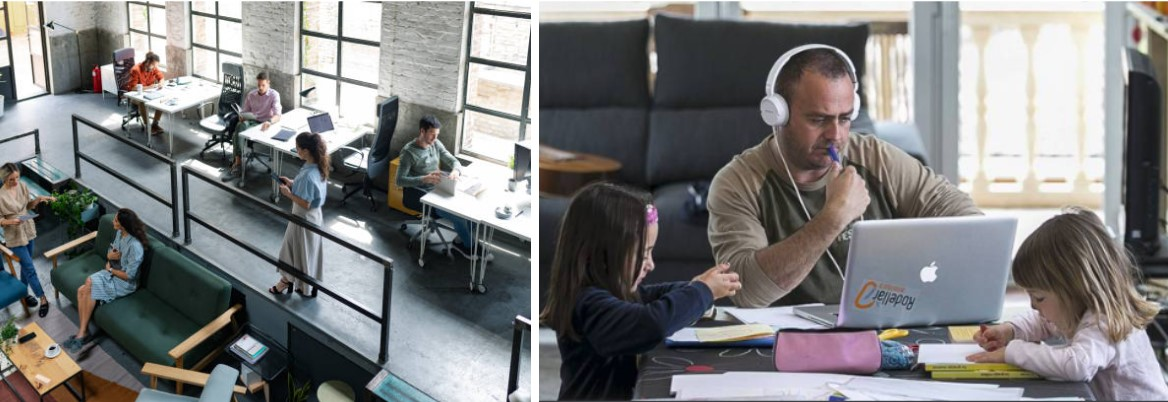
\includegraphics[width=1\textwidth]{./figuras/coworking_vs_homeoffice}
\caption{Coworking\cite{i_coworking} vs home office\cite{i_family}}
\label{F:coworking_vs_homeoffice}
\end{center}
\end{figure}

Aunque estas palabras son similares su uso técnico tiene diferencias significativas e implicaciones legales diferentes. Hemos de separar conceptualmente 3 visiones diferentes y complementarias, la organizativa a la hora de realizar el trabajo (grupo de trabajo), la situación física del trabajador y el carácter legal del trabajador.

Existen empresas que no tienen una sede física con oficina o tienen múltiples, las hay que mandan a sus trabajadores a las oficinas de sus clientes. En cualquiera de estos casos, estos trabajadores realizan el 100\% de su trabajo en remoto, puesto el grupo de trabajo no está reunido completamente en la misma oficina física, pero ninguno lo realiza desde su casa o consta como teletrabajo legalmente, puesto que se desplazan a la oficina que su compañía les indica.

Por otra parte, también existen muchas compañías que ofrecen flexibilidad horaria y la posibilidad de ‘teletrabajar’ dentro de su pack de conciliación. Que el trabajador pueda salir antes de la oficina y terminar un porcentaje de jornada desde casa (o cualquier otro lugar) con el fin facilitar su conciliación trabajo-vida familiar.

 Por último tenemos el caso de muchos trabajadores, especialmente mandos intermedios o especialistas cuyos proyectos con picos de trabajo realizan horas extras “trabajando desde casa”.

Desde el punto de vista técnico, \textbf{trabajar en remoto}, se refiere única y exclusivamente a realizar el trabajo (función dentro del grupo de trabajo) siendo exclusivamente dependiente de \textbf{medios virtuales}, es decir, el grupo de trabajo no está físicamente en contacto directo, no considera el lugar desde donde se realiza la actividad. Trabajar desde casa, o ‘\textbf{home office}’, indica que el trabajador dispone y realiza \textbf{un porcentaje significativo} (y mayoritario) de su trabajo en remoto, desde su vivienda habitual. Por último, \textbf{teletrabajar-legalmente} en España indica que el trabajador realiza más de un 30\% de su jornada laboral fuera de la oficina física de la empresa (ejemplo más 1.5 días a la semana o más de 2 horas 20 min diarias), o hasta un 50\% en contratos formativos.

Legalmente, el teletrabajo es voluntario, por lo tanto es un acuerdo fomentado por ambas partes. La empresa está obligada \cite{c_boe_teletrabajo} a firmar un contrato individual con el trabajador, donde se detallan los pormenores de la cesión de equipamiento y la compensación para los gastos ocasionados por el teletrabajo, así como los plazos, renovaciones y la posibilidad del cambio de dichas condiciones. Habitualmente suele quedar negociado dentro del convenio sindical, indicando que equipos o coworking designados y la cuantía mensual extra asociada a los gastos generados o con un presupuesto máximo preestablecido para nuevas incorporaciones. 

Esto en la gran  mayoría de casos suele plasmarse con “un acuerdo individual” basado en el convenio colectivo, usualmente con un portátil más todo aquel material que permiten llevar de la oficina a tu casa o una lista de elementos a comprar que la empresa te enviará a casa.


\section{Objetivo del teletrabajo}

Múltiples empresas han acabado implementado el teletrabajo, cada una por motivos diferentes\cite{c_work_remote_eurofound}, entre los principales objetivos y beneficios son los siguientes:
\begin{itemize}
    \item Productividad, principalmente relacionada con la mayor concentración de sus trabajadores en ambientes sin ruido ni interrupciones, junto a un uso más eficaz de su jornada al reducir el estrés de desplazarse a las oficinas y reducción de  tiempos perdidos o incidentes (atascos, meteorología, aglomeraciones ...).
    \item Flexibilidad extendida, principalmente focalizada en la conciliación familiar. “Un trabajador feliz” no solo es más productivo, es retener talento.
    \item Trabajadores des localizados, permite adquirir una plantilla no geo-localizada en una región local. Permite captar más talento, ya que el lugar de residencia no es requisito indispensable. Permite equilibrar salarial mente, aquellos lugares con rentas especialmente altas asociadas a grandes metrópolis.
    \item Reducción de costes asociados a la infraestructura física de las oficinas o servicios auxiliares de las mismas. Normalmente la reducción de costes en oficina física es superior a los acuerdos compensatorios de teletrabajo.
    \item Causa mayor, en algunas ocasiones eventos especiales, circunstancias climáticas-locales, situaciones político-sociales o causas médicas, no permiten la realización de la actividad laboral, siendo el teletrabajo la única opción.
\end{itemize}
Por otra parte requiere de una gestión o problemática asociada a la no interacción física, así como el \textbf{no uso} del “lenguaje no verbal” o comportamientos de grupos, difíciles de crear \textbf{sin un trabajo previo no remoto}. Por lo tanto existe las siguientes problemáticas:
\begin{enumerate}
    \item Mala gestión humana, recae en fuga de talento o bajada de productividad.
    \item Bajada generalizada de la creatividad y cohesión en equipos sin encuentros físicos.
    \item Requiere de una gestión jerárquica más directa y plana, así como una supervisión facilitada por ambos lados.
\end{enumerate}

\section{Histórico}
El trabajo en remoto existe hace décadas, especialmente desde la llegada del teléfono y los tele-operadores, pero para nuestra actual comprensión teletrabajar, está íntimamente ligado a trabajar con elementos tecnológicos que desde los años 90 permiten conectarse entre ellos y trabajar directamente con herramientas virtuales en constante comunicación.

Sin embargo ha sido una excepción de una élite muy especializada hasta la llegada de la banda ancha generalizada. No solo a sectores concretos sino también delimitado a regiones densamente pobladas y desarrolladas donde la conexión cumplía con los requisitos adecuados. 

\subsection{Pre pandemia}
Desde 2015 se observa un crecimiento significativo hasta el 5-15\%\cite{c_oecd_productividad_telework} en países desarrollados y la aparición de teletrabajo-des localizado especialmente en externalizaciones y freelance en países más competitivos salarial mente. Ambos casos se focalizan en una necesidad empresarial de obtener empleados cualificados, en un contexto de falta de personal y burbuja salarial.

Las principales características de estos trabajos son la flexibilidad familiar, la formación y la gratuidad de ciertos complementos con el fin del acceso a una mayor  disponibilidad de empleados cualificados que pueden realizar gran parte de su jornada laboral desde casa.

\subsection{Pandemia}
La pandemia covid-19 supuso en 2020-21 un verdadero experimento global que forzó por causas mayores\cite{c_boe_pandemia} el uso de teletrabajo en una gran parte de la población debido a las restricciones médicas. Aunque en algunas empresas especialmente de oficinas el teletrabajo ascendió por encima del 80\%, la realidad es que esta puesta acelerada donde destacaron la falta de medios, herramientas y organizaciones jerárquicas no preparadas para ello.
Desde mi punto de vista, los análisis y datos de este experimento social están muy sesgados por las circunstancias y recursos asociados a los empleados teletrabajando durante esos dos años. Especialmente llama la atención como grupos principalmente personas del sector tecnológico, sin cargas familiares y con unos recursos tecnológicos “semi-preparados” aumentaban significativamente la productividad y satisfacción. Mientras en otros con cargas familiares como niños o sin el adecuado espacio de trabajo lastraban su productividad y satisfacción. Por otra parte es complejo de evaluar, ya que muchas publicaciones son meramente estadísticas y no evalúan la formación y actuación de los mandos intermedios, ya que \textbf{gestionar empleados en remoto  es algo totalmente distinto}.

\subsection{Post Pandemia}
Actualmente dependiendo de qué país, pero especialmente de qué tipo de empresa, se están decidiendo cambios en el teletrabajo, especialmente de origen político-cultural, es decir, no especialmente racionales o justificables. Se han detectado patrones de comportamientos completamente opuestos, mientras hay empresas que insisten en una bajada de la productividad global, otras muestran una subida, generando tres tendencias:
\begin{itemize}
    \item Expansión y estandarización del trabajo en remoto, especialmente en empresas pequeñas, donde la cultura de objetivos y la digitalización favorece el debate ante una productividad mejorada o equilibrada con la reducción de costes asociados al teletrabajo. 

    \item Trabajo híbrido, especialmente en aquellas empresas de gran tamaño que han obtenido resultados contradictorios en sus diferentes grupos de trabajo. Intenta solventar las demandas de teletrabajo de sus trabajadores y la fuga de talento con la baja productividad o mala gestión de los mismos, con cuotas mínimas de días en oficina.

    \item Vuelta a la oficina, gran cantidad de empresas especialmente de gran tamaño, han optado por la vuelta irremediable a la oficina cambiando el teletrabajo, por flexibilidad, es decir inferior al 30\% de la jornada laboral.

\end{itemize}
Interesante es el colapso de servicios, principalmente en empresa o entes públicos, cuyas productividades ya eran bajas previamente a la pandemia,  han colapsado ante el teletrabajo favorecido por la administración, ya sea por una productividad aún menor o una falta de medios, organización o la falta de atención pública adecuada, parece estar destinada como ejemplo de cómo no implementar el teletrabajo.

\subsection{Opinión Personal}
Primero de todo he de indicar que aunque soy partidario del teletrabajo 100\% remoto, aceptó ampliamente la necesidad de 1 o más días en oficina y me interesa especialmente destacar ciertos puntos que no están en el actual debate de “teletrabajo vs oficina”.

El teletrabajo es una herramienta que debe facilitar la labor del trabajador, pero también los resultados para la empresa. Por ello debe cumplir un conjunto de requisitos si queremos que se utilice adecuadamente. La empresa debe proporcionar los medios tanto físicos como digitales para realizarlos, pero una parte importante recae en el trabajador, no solo a la hora de preparar su ambiente de trabajo sino de separar y auto-gestionar su manera de trabajar de su vida personal.

Los mandos intermedios y las dinámicas de equipo deben ser apropiadamente actualizadas para evitar la falta de cohesión, la baja producción o falta de tareas, y el abandono de las personas nuevas, quienes sin una presencialidad y formación no pueden rendir como un trabajador ya formado y cohesionado dentro del equipo.

En mi opinión las estadísticas del teletrabajo enmascaran comportamientos no adecuados dentro del grupo de trabajo. Especialmente aquellos trabajadores que no producen ni rinden cuentas de su trabajo, o nuevas incorporaciones que no saben, no conocen o no interactúan con el equipo, no aprendiendo ni produciendo adecuadamente. 

En definitiva el teletrabajo no solo es una herramienta que ayuda a conciliar, hace evidente quien trabaja y quien no, donde existe una gestión de equipo planificada o no;  y donde hay un equipo cohesionado o fraccionado. 

Por ello muchas veces la presencialidad es necesaria para solucionar un problema; la dedicación de un día presencial cada 1-3 semanas para el equipo es necesario. Así como la dedicación de varias semanas con presencialidad para aquellos senior y junior involucrados en la formación de nuevas incorporaciones. Por último filosofías como SCRUM, e indicadores  (chat, correos, commits, horas conectado) pueden ayudar generar índices de actividad que detecten cuando existe un problema, no solo de baja productividad sino de sobrecarga de trabajo o estrés, también excesivamente habitual en teletrabajo que tarde o temprano derivara en una baja productividad por “el síndrome del trabajador quemado”\cite{c_trabajador_quemado}.

En mi opinión, hay que evaluar las tendencias a largo plazo, segmentando cada caso con su peculiaridad y evaluando de manera continua como mejorar o mantener no solo una productividad óptima sino una satisfacción continuada.

\section{Ofertas laborales}
Actualmente podemos observar la siguiente amalgama de ofertas laborales que integran la palabra “teletrabajo”:
\begin{itemize}
    \item “Flex work”: trabajo flexible, condiciones flexibles en el horario de trabajo así como un máximo de 30\% fuera de la oficina. No es teletrabajo legalmente en España.

    \item “Telecommuting”: se refiere principalmente a trabajadores que realizan su trabajo a distancia, principalmente focalizados en clientes. Aunque la traducción es “teletrabajo” se refiere principalmente a ventas o personal de enlace que viaja regularmente. En muchos casos aplican un 50-20-30, la mitad de la jornada trabajan desde casa, 20\% en la oficina de la empresa y 30\% en viajes o reuniones con clientes.
    
    \item “Partial remote”: Aplica a teletrabajo-legal, indica que es obligatorio asistir al menos 1/2/3 día a la semana y suele combinarse con “flex work”. Es el más utilizado sobre todo en metrópolis, donde el objetivo es minimizar los desplazamientos y mantener a una plantilla “metropolitana” o local. Permite reducir el tamaño de la oficina.

    \item “Work on Objectives”: ofrecen a sus trabajadores aquellas modalidades que ellos más deseen. El único objetivo de la empresa consiste en que las entregas y objetivos se cumplan dando libertad al equipo para auto-gestionar su forma de trabajar.
    
    \item “Full remote”: Esta modalidad indica que para realizar la actividad laboral no es necesario ir a la oficina. Sin embargo, normalmente se realizan reuniones periódicas cada 2/3/4 semanas con el fin de sincronizar, facilitar la comunicación y cohesionar el equipo. Los trabajadores pertenecen a un mismo país o región (4-6 horas-distancia). La oficina está pensada como lugar de encuentro no de trabajo intensivo.
    
    \item “International Full remote”: Aplica la modalidad “full remote” internacionalmente, por lo que las reuniones presenciales son escasas o trimestrales. Suelen generarse grupos regionales que quedan para cohesionar equipo y realizar reuniones físicamente-parciales, pero online entre los diferentes subgrupos.
    
    \item “Remote Freelance”: Personas que se dedican a colaborar o realizar pequeños trabajos. Trabajan en remoto mayoritariamente, desde su casa, pero ocasionalmente se desplazan al cliente para acordar entregar y establecer la dinámica de trabajo. Similar al “work on objectives” y al “full remote” su característica principal es la autogestión y la participación como trabajador externo dentro del grupo de trabajo. Legalmente no son teletrabajadores ya que actúan como trabajadores por cuenta ajena (coloquialmente llamados autónomos en remoto).
    
\end{itemize}

\section{Teletrabajo overemployed}
Desde 2021, se ha hablado de manera abierta del 'overemployed', focalizado en personas que teletrabajan en dos trabajos. No es el objetivo de este documento evaluar la ética o profesionalidad de dichas casuísticas, por lo que entendemos que el contexto es legal, no solapada y en muchos casos el 2º trabajo es dedicación personar a una empresa propia.

Es de interés\cite{c_overemployed} que en muchos de estos casos, la infraestructura física, así como el aislamientos cibernético, red, dispositivos, vpn, en muchos casos se acerca al nivel teórico remalcado por este documento, especialmente entre la separación y uso del setup para usos personales y profesionales. Gran cantidad de periféricos, estrategias y softwares-herramientas se han solapado con los requisitos de este documento.



\section{Caso de estudio}
En este trabajo nos interesa aquellos casos donde existe una realidad de teletrabajo-legal, y dicho trabajador realiza mayoritariamente su actividad desde casa ya que son aquellos que mayor desafío y problemática generan con unos requisitos superiores tanto a nivel de setup, espacio como de herramientas de trabajo.

Por simplicidad así como afinidad a la profesión de este autor, se focaliza en la aplicación directa sobre Ingenieros realizando tareas de desarrollo, principalmente software pero fácilmente aplicable a diseños electrónicos, planos, prototipado y automatizaciones. De igual manera otras profesiones como diseñador gráfico, montaje audiovisual y soporte de incidencias tiene un solapamiento claro en la gran mayoría de requisitos.

\chapter{Requisitos y oficina física}\label{S:anexo_B}
Este anexo contiene las explicaciones, comparativas y conclusiones parciales relacionadas con la creación de una oficina física, hardware así como la documentación fotográfica y otros detalles de la implementación real de “mi oficina” como desarrollo práctico del capítulo \ref{S:tema_1}.

\section{Definición y tipos de requisitos}\label{S:requisitos}

Definición de “\textbf{mínimo}”, entendemos un requisito de mínimos aquellos que permiten realizar el trabajo no exentos de problemática y repercutiendo en la performance o agilidad durante el trabajo. Ejemplos que permiten trabajar de manera “mínima” son aquellos donde tenemos un pc/laptop  y una o varias de las siguientes casuísticas:
\begin{itemize}
    \item Mesa y silla, no especializada y compartida para otros usos.
    
    \item Un pc/laptop que no cumple los requisitos mínimos para hacer el trabajo de manera holgada y afecta negativamente tanto en su uso como en el tiempo requerido.
    
    \item Un espacio de trabajo compartido, ruidoso, con constantes interrupciones ajenas al desarrollo profesional.
    
    \item Conexión de internet insuficiente, que limita las comunicaciones y retrasa significativamente el trabajo.
    
\end{itemize}

Definición de “adecuado”, este apartado puede variar en función de la especialización del trabajo a realizar. Mientras un soporte de incidencias necesita de unos requisitos de hardware básicos, buena conectividad; un renderizado de imagen/vídeo puede necesitar de un hardware potente y una conexión mediocre. Por lo tanto, se sobreentiende que la definición promedio debe estar sensiblemente acoplada a la actividad a realizar. Como se ha mencionado en nuestro contexto nos focalizamos en la creación o gestión de software.

Un  requisito “\textbf{adecuado}” debe permitir una mejora sustancial del 30-40\% en las tareas a realizar sobre un requisito de “mínimo” y permitir evitar la gran mayoría de puntos negativos, que pueden degradar o repercutir no solo la realización y calidad de trabajo sino las comodidad y satisfacción del trabajador.

Un  requisito “\textbf{óptimo}”, depende en gran medida de la especialización y los gustos del propio trabajador, incrementa normalmente la satisfacción del trabajador aunque no es una mejora sustancial en la productividad del trabajo intrínseco.

De una manera muy similar podemos hablar de 4 amalgamas presupuestarias, “\textbf{básico}” usualmente acoplada a la definición de “\textbf{mínimo}”, “\textbf{profesional}” focalizada en calidad precio cumpliendo los requisitos de “\textbf{adecuado}”, “\textbf{profesional pro}” excede los requisitos de adecuado y se acerca a “\textbf{óptimo}” a un precio justificado y finalmente “\textbf{business}”, excede no sólo los requisitos de óptimo y normalmente malgasta recursos o opta por acabados y marcas de mayor prestigio que no aportan mejoras medibles.

\section{Requisitos físicos}

Este apartado evalúa y compara diferentes niveles mínimos/adecuados/óptimos como requisito físicos, es decir, elementos de hardware, espacio e instalaciones para la realización de un trabajo profesional.

\subsection{Área de Trabajo}
Un cubículo público como el que podemos encontrar en las bibliotecas de la UPC (fig. \ref{F:cubiculo_upc}) es el área de trabajo mínima. Un área de trabajo de menos de 1 metro cuadrado capaz de almacenar un portátil y documentación auxiliar, conectividad WIFI, alimentación eléctrica, una silla y como se aprecia en la imagen un área personal aprox. de otro metro cuadrado que en muchos casos delimitada por biombos, marquesinas o cristales translúcidos. 

\begin{figure}[htb]
\begin{center}
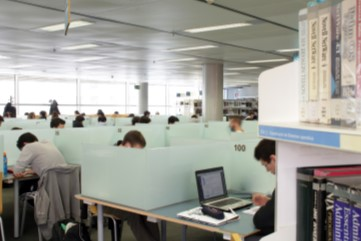
\includegraphics[width=0.75\textwidth]{./figuras/cubiculo_upc}
\caption{Cubículo biblioteca UPC (campus nord)}
\label{F:cubiculo_upc}
\end{center}
\end{figure}

El objetivo de esta área no solo es soportar los elementos de trabajo, sino aislar de distracciones o interacción social al trabajador. Usaremos este cubículo como definición mínima, duplicaremos los requisitos para adecuada y generalizamos en una habitación o pseudo habitación reservada como óptima.

Iluminación artificial (mínimo), compaginada con luz natural (adecuado), luz regulable, persianas, estores, tanto natural como artificial (óptima).

 Ventilación diaria manual (mínimo), ventilación natural o automática (adecuado), espacio aclimatado con filtros, regulador de humedad y porcentaje de aire externo (óptimo).

 \subsection{Otros elementos}

 Es de importancia significativa la selección de mobiliario y elementos auxiliares tales como alfombrillas (mínimo), mesa o escritorio no especializadas (mínimo), escritorio de más 70 cm de altura o regulable (adecuado), mesa-escritorio especializada motorizada que permite trabajar de pie (óptimo).

\begin{figure}[htb]
\begin{center}
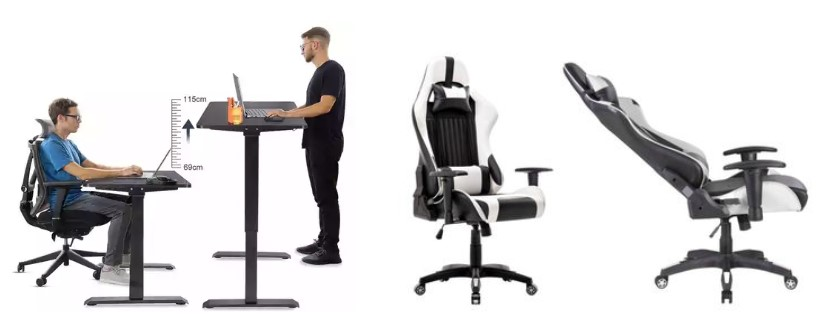
\includegraphics[width=1\textwidth]{./figuras/amazon_sillas}
\caption{Silla y mesas, productos Amazon.}
\label{F:amazon_sillas}
\end{center}
\end{figure}

Silla ergonómica básica (mínimo), silla ergonómica ajustable con cojín lumbar (adecuado), silla gamer o business (óptimo).

\begin{figure}[htb]
\begin{center}
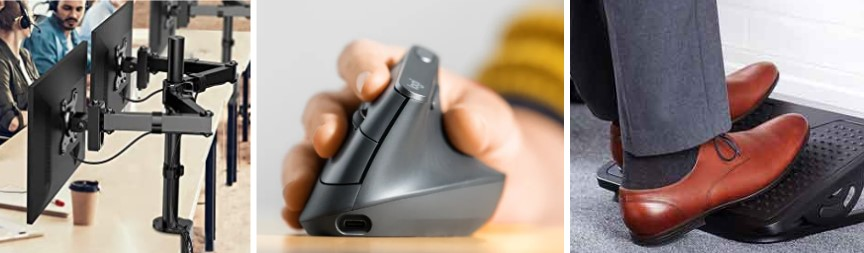
\includegraphics[width=1\textwidth]{./figuras/amazon_extras}
\caption{Porta monitor, raton ergonómico, productos Amazon.}
\label{F:amazon_extras}
\end{center}
\end{figure}

Elemento opcionales como, reposapiés (adecuado), ratón ergonómico / almohadilla con reposa muñecas (adecuado), eleva monitores (adecuado), porta monitor ajustable(óptimo). Debe entenderse que no solo es una cuestión de comodidad, sino que repercute seriamente en la salud de los trabajadores, y por consiguiente en el porcentaje de absentismo laboral generando un problema de salud crónico o reiterativo.

\section{Setup informático}\label{S:setup_informatico}

El setup informática es el corazón de la oficina, ya que es la principal herramienta en torno a la cual giran el resto de requisitos. Además es el elemento más customizable y en el que hay menor consenso, ya que puede ser evaluado económicamente, por mantenimiento, actualización e interoperabilidad.

\subsection{¿Cuál es tu prioridad?}
Primero de todo existe una difícil decisión basada en la movilidad y el mantenimiento. Podemos disponer de un laptop que ofrezca rendimientos “adecuado” a precios “profesionales” con una movilidad e interoperabilidad a través de hubs o docking stations.

También podemos disponer de torre o semi torre comúnmente llamada PC, cuyo hardware-precio tiene mayor cantidad de recursos a menor precio fácilmente ampliable o mantenible pero requieren de un espacio dedicado y tiene nula movilidad.

\begin{figure}[htb]
\begin{center}
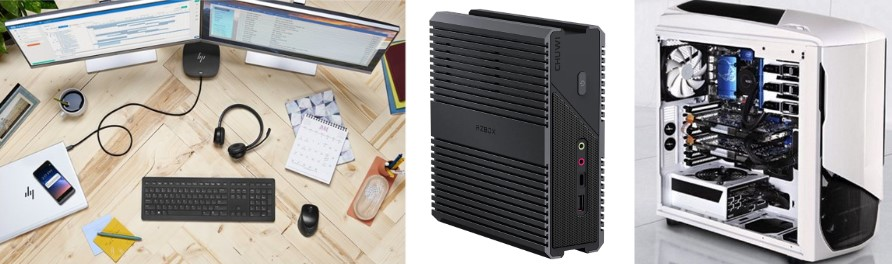
\includegraphics[width=1\textwidth]{./figuras/laptop_minipc_torre.jpg}
\caption{Portátil, mini pc y torre, google images. }
\label{F:laptop_minipc_torre}
\end{center}
\end{figure}

Por último tenemos los mini-pc o torres-slim, contienen un hardware potente para uso 'adecuado', poco actualizable pero muy asequible, además de un volumen reducido y la posibilidad de ser reubicado fácilmente, sin tener la autonomía de un laptop.

Ante un presupuesto fijado a 6-8 años vista, se pueden emplear dos estrategias, 'hardware potente mantenido', o el uso de 'hardware medio pero reemplazable' a 3-4 años, siendo presupuestaria mente equivalentes.

Como recomendación de este autor adoptó ampliamente del uso portátil como elemento más interdisciplinar, autónomo y de fácil uso. Sin embargo para aquellas startups o oficinas físicas el uso de mini-pc puede ser un nicho muy interesante. La estrategia de reemplazo dependen de las circunstancias tecnológicas del mercado en el momento de la compra que son explicadas en los apartados de CPU y RAM.

\subsection{Pantalla, comodidad y opinión}\label{S:pantallas}
Tenemos 'el dilema del tamaño, forma y número de pantallas'; no existe un consenso claro, excepto de que es necesario 1 o más monitorios para trabajar “adecuadamente”, es decir, la pantalla del laptop más un monitor extendido; una gran pantalla o dos pantallas en caso de pc o mini-pc. 

Existe un gran debate sobre si la disposición de los monitores debe ser 16:9 en tamaño de 21’-24’/27’ o de 21:9 en 30’-34’ pulgadas. Mi punto de vista es:  dos pantallas en caso de pc; depende del espacio, presupuesto y tamaño en el caso de laptop.

\begin{figure}[!htb]
\begin{center}
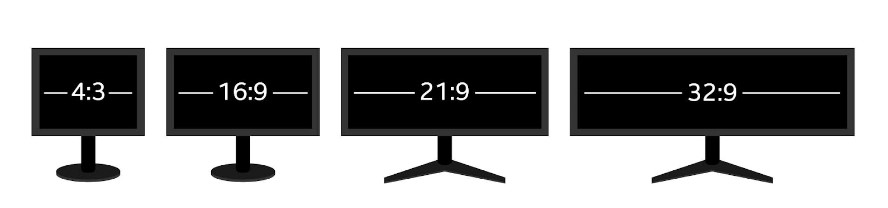
\includegraphics[width=1\textwidth]{./figuras/pantallas_geometria.jpg}
\caption{Monitores, formas y geometrías \cite{i_pantallas}. }
\label{F:pantallas_geometria}
\end{center}
\end{figure}

En mi opinión, si el portátil es “versátil” en movilidad, no supera las 13’-15’ por lo que requiere dos pantallas como un pc, de 24’ o 27’ ambas con las mismas características. Si el portátil tiene una pantalla “adecuada” para trabajar 16’-17’, puede elegir una única pantalla extendida, siendo recomendable 30’-34’ disposición 21:9.

La realidad es que si el presupuesto y el espacio lo permite, he llegado a ver el uso de 3 y 4 pantallas obviando la propia del portátil.

Requisitos indispensables son la resolución mínima FHD (1920x1080), adecuada QHD (2K) y óptima UHD (4k) , tecnologías “eye care” y una frecuencia alta 60-75 hz (adecuado) para reducir el esfuerzo visual. Cualquier otro detalle fuera de estos queda catalogado como customización en función del precio-calidad, ya que mejoras sensibles en las pantallas con un gran presupuesto pueden quedar totalmente degradadas con una inadecuada iluminación ambiental.

\begin{figure}[!htb]
\begin{center}
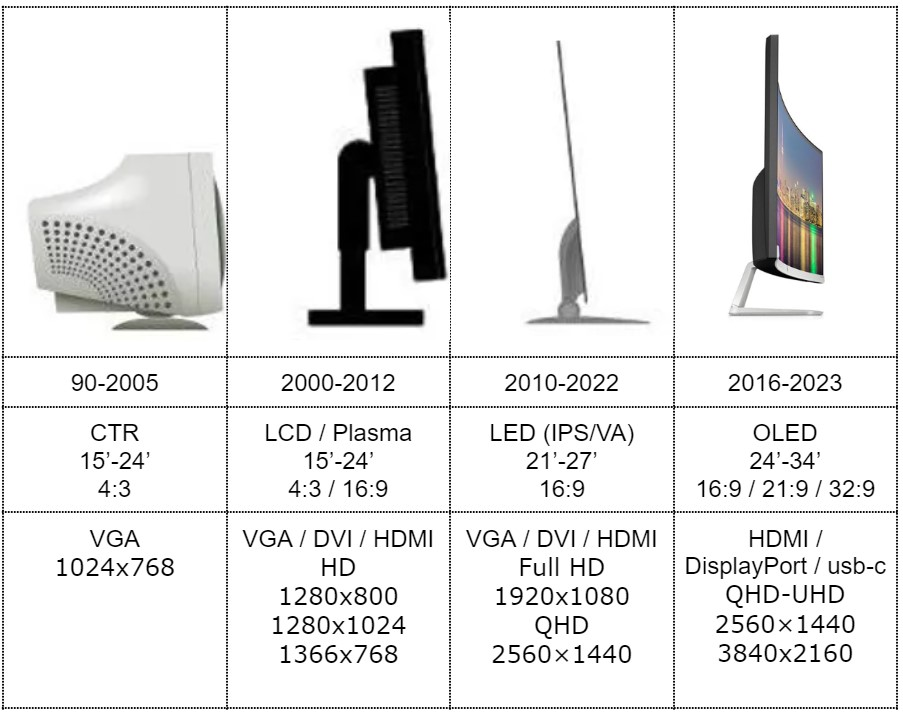
\includegraphics[width=1\textwidth]{./figuras/comparacion_monitor_tech.jpg}
\caption{ Evolución tecnológica monitores ultimos 30 años.}
\label{F:comparacion_monitor_tech}
\end{center}
\end{figure}

Importante resaltar (véase fig. \ref{F:comparacion_monitor_tech}) que el mundo de los monitores, evoluciona más lentamente en una perspectiva 5-10 años, donde la vida media de una pantalla excede los 12 años, por lo que suelen reemplazarse tecnológicamente cuando superan los 10 años por calidad en relación a sus prestaciones-precio.

Por lo tanto no es una cuestión de requisitos mínimos, sino de una tendencia económica, donde a un rango de precio “profesional” evoluciona con mejoras técnicas (resolución, tecnología, espacio-forma) a un precio equivalente. Como dato re-marcable\cite{c_resolucion_estadisticas_W3Schools} las pantallas más compradas en 2020-22 fueron 24’, 27’, 32’ con resolución FullHD, así como la resolución más utilizada en webs de programadores fueron 40\% superiores Full HD, 20\% Full HD y 30\% inferiores.

Como conclusión entenderemos que \textbf{no tiene sentido reemplazar los monitores con menos de 5 años}, así como \textbf{suele ser práctico-económico a partir de los 8 años}, pero se puede trabajar adecuadamente con ellos hasta el final de su vida útil 12 años, que es lo que reflejan las estadísticas de resolución utilizada en navegadores.

\subsection{Hardware y recursos}\label{S:hardware_recursos}
El hardware y recursos empleados evolucionan en el tiempo (a una velocidad más rápida que los monitores), la vida media de un setup actual es de \textbf{4-6 años}, no superando los 8 años, durante los cuales es necesario un mínimo de actualizaciones, mantenimiento o reemplazo de piezas. Así mismo la usabilidad se resiente especialmente en baterías o equipos sin el apropiado mantenimiento.

Actualmente la gran mayoría de PC de 2010-2013 aún están en funcionamiento, 10 años después, algo verdaderamente improbable en los años 80 's, 90' s,  o principios de 2000.

 La realidad es que se ha ganado en rapidez y cantidad pero especialmente en multitasking, especialmente en programas de grandes volúmenes de datos, es decir, ‘más cantidad que calidad’. Por lo que los requisitos tanto del sistema operativo como de los programas más comunes son ampliamente movidos por hardware viejo. Por otro lado, el espacio en disco o la velocidad de acceso, así como la memoria RAM evolucionan continuamente aumentando velocidades y capacidades a un coste inferior, lo cual ha permitido mejorar los cuellos de botella en aquellos hardwares viejos con actualizaciones sencillas véase \cite{c_guia_hardware}. Este punto debe aclararnos que el mantenimiento es un elemento muy critico, especialmente si esperamos extender la vida del hardware 8-12 años para otras tareas no profesionales.

 \subsection{Periféricos}
 Entendemos como periféricos aquellos elementos externos que usualmente se conectan por USB o bluetooth. Un hub de conectividad o hub de monitor externo es obligatorio, así como se sobreentiende un ratón y teclado. Existen varios elementos dignos de mencionar en la catalogación de los mismos:
 \begin{itemize}
     \item Auriculares y uso del micrófono-cámara del portátil (mínimo). Auriculares de alta calidad con micrófono (adecuado), auriculares con cancelación de ruido y micrófonos HD (óptimo), web-cam HD con micrófono con cancelación de ruidos (óptimo).
     \item Plataforma de elevación laptop (adecuado), plataforma hub con refrigeración activa laptop (óptimo).
     \item Sistemas de autenticación externos, lector de huellas, lector de tarjeta etc…. (óptimo).
     \item Panel táctil y bolígrafo asociado (óptimo), pantalla táctiles asociada a monitor o laptop (óptimo).
     \item Google home, Alexa, u otros elementos de domótica, automatización, fuentes musicales o notificaciones. (óptimo, pero requiere de análisis riesgos de seguridad).

     \item Requerimientos especiales, impresora-scaner, impresoras 3d, electrónica de monitorización o placas prototipado. (solo bajo necesidad práctica).
 \end{itemize}

  \subsection{Gestión del setup}
  Existe una norma bastante compleja ya que la gestiona cada individuo, cuyo objetivo es separar el trabajo de tu vida personal. En muchos casos aunque un despacho o habitación dedicada a tu setup sirve como jaula de aislamientos y concentración. La realidad es que gran cantidad de profesionales tiene intereses alineados o coincidentes con sus labores profesionales y de igual manera tiene sus necesidades personales de acceso a la información, cuentas personales, almacenamientos, documentos y juegos.

¿Cómo separar el pc personal del profesional?

Un buen profesional no debe usar su setup profesional para usos personales, primero para mantener esta estricta separación que no afecte o predisponga a distracciones de índole personal durante la jornada laboral. Por otra parte están los riesgos de ciber seguridad de generar un agujero de seguridad desde sus cuentas personales a sus servicios profesionales.

\subsubsection{Aislamiento de navegación}
La gran mayoría de servicios personales a día de hoy son capaces de ser usados vía navegador, así como el acceso a noticias, comunicaciones en línea y servicios streaming como pueden ser música. La primera capa de seguridad es separar y la gestión de nuestras cuentas personales y profesionales en diferentes cuentas de sincronización. Permitiendo acceder a dos cuentas vía nuestro navegador, y evitando almacenar contraseñas, historial de navegación, cookies y otros elementos. Una separación más estable es el uso de diferentes navegadores para cada una de las cuentas, así evitamos una gestión compleja o la afectación de plugins inseguros en el navegador.

En mi opinión son una buena opción, aunque solo debe usarse en momentos de necesidad y debe evitarse lo máximo posible.

La opción más adecuada para dichos casos tales como revisar mails, esperar un mensaje vía whatsapp o simplemente poner tu playlist de relajación en los altavoces pasa por el uso de \textbf{un 2º elemento personal móvil/tablet/laptop} capaz de surtir dicha función sin necesidad de usar tu hardware profesional e \textbf{incluso utilizando diferentes redes} para conectarse.

\subsubsection{Setup Conmutable}
Sin embargo qué hacemos cuando en la post jornada laboral deseo trabajar en mi hobby tecnológico, o simplemente jugar o ver series desde mi pc personal.¿Debo acaso duplicar recursos teniendo un precioso despacho con un setup con múltiples pantallas?

La respuesta es simple; \textbf{No}. Si seleccionamos adecuadamente los monitores a elegir, así como el dock-station o hub de periféricos, pronto entenderemos que es fácil disponer de hasta 3 o 4 fuentes de imagen independientes, múltiples fuentes de sonido y un uso compartido de periféricos. 

\begin{figure}[!htb]
\begin{center}
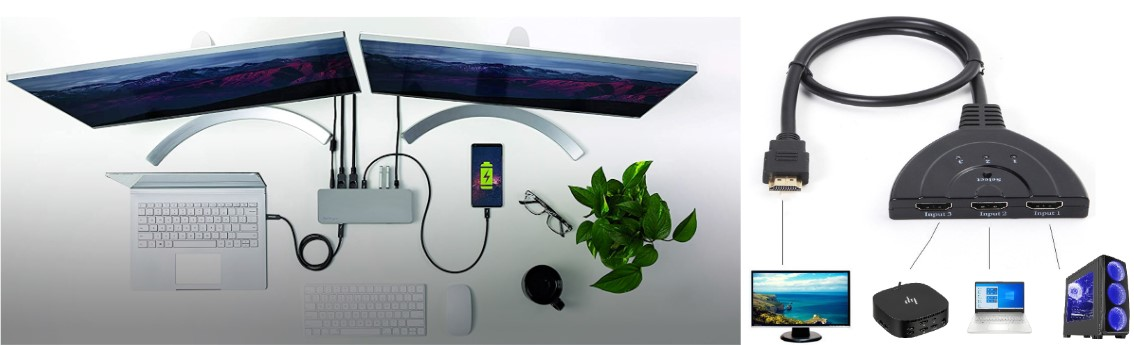
\includegraphics[width=1\textwidth]{./figuras/conectividad_monitores.jpg}
\caption{ Conectividad de monitores, amazon products.}
\label{F:conectividad_monitores}
\end{center}
\end{figure}

Se puede optar por la estrategia centralista, todo se conecta a nuestro hub y con conmutar la conexión usb hub-portátil de laptop profesional a personal ya tenemos el setup completo para uso personal. O se puede seguir una estrategia de fuentes en paralelo, de tal manera que ambos hardware están conectados a puertos diferentes o a través de un multiplexor. Si solo uno está encendido, basta con cambiar de pc/laptop el usb que controla el teclado-ratón o el hub de usb y ya podemos utilizar el setup. Si ambos están encendido, requiere seleccionar en las pantallas la fuente a mostrar y conectar el teclado-ratón aquel que queramos usar.

En mi opinión la segunda opción es más interesante aunque compleja, requiere de una mayor planificación, pero facilita la simultaneidad de 3 o 4 pc, pudiendo estar conectado en sesiones en remoto desde aquel que gestione las pantallas.

\section{Abastecimientos auxiliares}\label{S:abastecimientos_auxiliares}
Abastecimiento auxiliares, son todas aquellas infraestructuras o herramientas necesarias para poder usar nuestro setup adecuadamente. Entre las principales necesidades tenemos los suministros de electricidad, climatización y acceso a internet. Otros interesantes son aquellos que usamos como alternativa funcional cuando un suministro básico falla, sistemas de alimentación ininterrumpida (SAI) o equivalentes, acceso alternativo a la red, setup mínimo alternativo o una planificación aceptable en caso de NO poder realizar home office. 

\subsection{Suministro Eléctrico}
Este elemento parece simple y obviamente necesario, pero a parte de la disponibilidad de red eléctrica y de la partida compensatoria en el acuerdo de teletrabajo qué implicaciones tiene en nuestro oficina el suministro eléctrico.

Disponibilidad de enchufes o switch, verdaderamente es complejo alimentar 2 pantallas, un hub, un portátil, una lámpara y algún que otro periférico extra. Aun lo es más si el sistema eléctrico es viejo y el único enchufe disponible tiene una amalgama de extensores-ladrones interconectados entre ellos. Recordemos que los enchufes tradicionales tienen 10-16A como límite, así como muchos 'alargos' no utilizan cable de 2.5 $mm^{2}$ sino 1.5 $mm^{2}$ de sección.

\begin{figure}[!htb]
\begin{center}
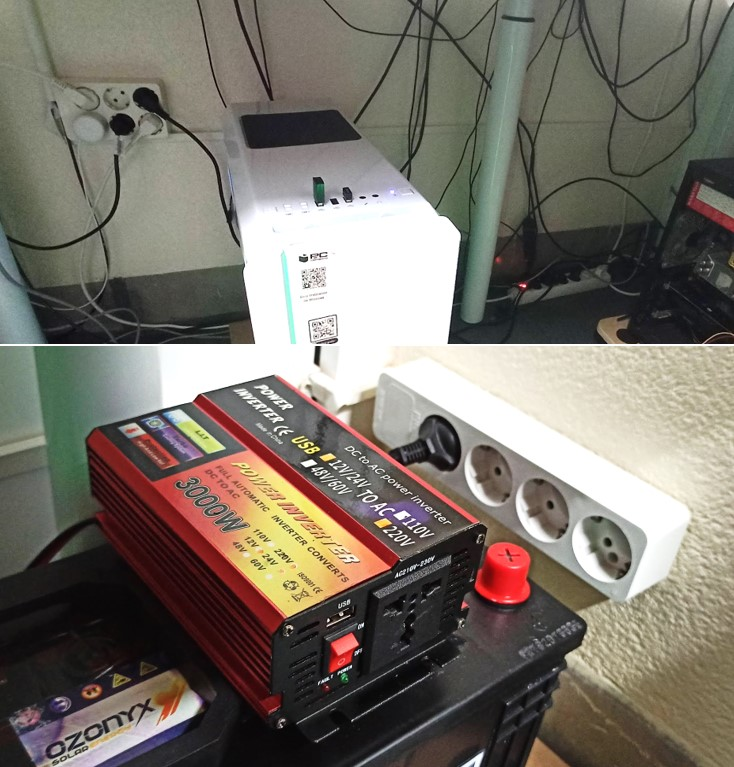
\includegraphics[width=0.75\textwidth]{./figuras/instalacion_electrica.jpg}
\caption{ Enchufes e instalación eléctrica.}
\label{F:instalacion_electrica}
\end{center}
\end{figure}

Como conclusión hemos de recordar que si bien un setup no es una actividad industrial requerirá de un mínimo de 6 enchufes-switch y raramente supera un consumo límite de una toma en torno a los 2000-2500W pero si puede ser un problema en una oficina de una startup afincada en un antiguo piso, especialmente cuando se usan elementos como calefactores o múltiples estaciones de trabajo no planificadas previamente. En dicho caso recomendamos no solo la instalación de múltiples switches con el cableado adecuado, sino el aislamiento de las filas o islas de trabajo, en PIAs\cite{c_pia} independientes con el fin de aislar y detectar fallos eléctricos que no afecten a la oficina de manera generalizada.

\subsection{Climatización}
Este punto tiene controversia entre oficinas como en gastos de teletrabajo. En mi opinión, la temperatura de trabajo óptima es un tema muy personal, sin embargo se recomienda entre 23º-27º en verano y 17º-24º en invierno. El verdadero punto importante es la existencia de una ventilación continuada y adecuada que reduzca los riesgos contaminantes, alérgenos y degradación de la calidad del aire.

Vivo en una zona privilegiada “Costa Daurada” de Tarragona cuyo invierno no baja de los 8º-10º y las temperaturas veraniegas raramente superan los 38º. Por lo que con apenas el aislamiento de la vivienda y una adecuada ventilación bien puede entrar dentro del intervalo de confianza de manera pasiva. Sin embargo nadie ha hablado de la humedad, la cual en la costa es siempre superior al 60\% (invierno) y mayor al 90-95\% (verano).

A su vez, un trabajo en remoto significa, poco movimiento físico y contacto continuado de extremidades con silla y escritorio, por lo que por experiencia propia puedo decir que no se puede trabajar adecuadamente con más de 28º en verano, ni menos de 18º en invierno, sea cual sea la ropa utilizada debido a la alta humedad ambiente y la naturaleza del trabajo.

Como conclusión los ventiladores o calefactores eléctricos son “mínimos”, un spliter de bomba calor frío “adecuado”, usar la aclimatación general de la casa “óptimo” pero costoso. En la instalación de la caseta se opto por un pingüino (bomba de calor/frió), sin embargo se ha desmantelado y sustituido vease mejoras de 2023 \ref{S:cambios_bombacalor}.

\subsection{Acceso a Internet}
Los requisitos de acceso a la red son un elemento crítico para el home office, no solo por las características necesarias sino porque dicho medio es compartido en la vivienda por los usos particulares de la familia. 
\begin{figure}[!htb]
\begin{center}
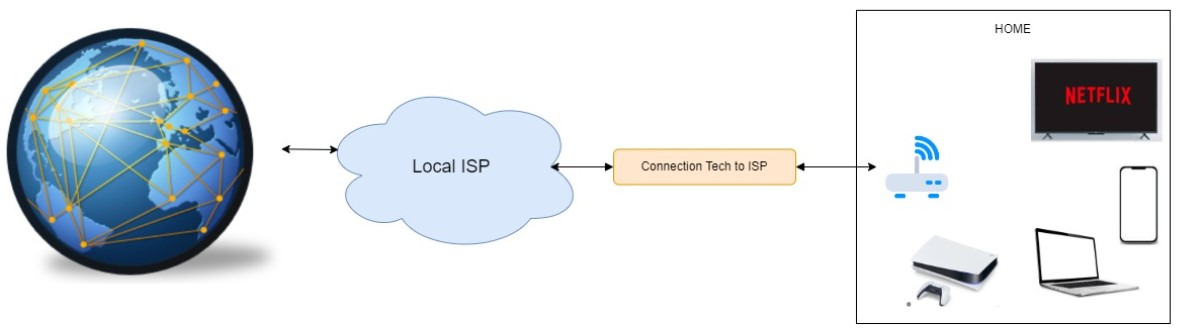
\includegraphics[width=1\textwidth]{./figuras/conexion.jpg}
\caption{Diagrama de conexión. }
\label{F:conexion}
\end{center}
\end{figure}
Por lo tanto la “velocidad” de la conexión debe permitir establecer videoconferencias junto al uso de streaming (netflix,spotify…) u otros usos personales de alta demanda. En la implementación física de mi oficina, usamos mi conexión familiar de 600 Mbps de fibra simétricos que escede ampliamente las necesidades.

\subsubsection{Ancho de banda}
Ancho de banda (BW), tasa o velocidad es la capacidad de transmisión de datos por segundo que permite la conexión de manera estable e ininterrumpidamente. Existen conexiones simétricas, velocidad de subida (uplink) y bajada (downlink) idénticas, y asimétrica donde la uplink suele ser inferior (entorno a un 20-30\% del downlink).

Una vídeo conferencia exigente, con múltiples usuarios enviando imagen y sonido HD con posibilidad de pantalla compartida, requiere de un mínimo de 4-8 Mbps. Una transmisión HD en netflix oscila entre 3-5 Mbps, 15 Mbps si es 4K. Se sobre entiende que en un contexto de coexistencia familiar y de posible ejecución en paralelo de más actividades profesionales, un uso mínimo  requiere una conexión de 10/3 Mbps (uplink/downlink), una conexión adecuada \textbf{15/5 Mbps} y una óptima son aquellas con tasas superiores a los 20/10 Mbps.

El ancho de banda de una conexión está intrínsecamente definido por la tecnología de acceso proveída por el ISP local, ejemplo conexión fibra movistar 100/100 Mbps. Pero influenciado por la congestión del ISP local o nodos intermedios, como ejemplo de las 100 megas simétricas, mi conectividad con diferentes servidores españoles puede ser de 60-80 Mbps (inferior a la conectividad directa con el ISP) y usualmente asimétrica, pero podemos obtener medidas de 15-30 Mbps con servidores asiáticos.

\subsubsection{Latencias}
La latencia, coloquialmente llamada lag o ping, es el tiempo medio de ida o vuelta en una conexión de red, es decir el tiempo mínimo de interacción entre dos elementos de la red. 

Las personas detectamos que la comunicación no es “instantánea”, si la interacción de dos interlocutores es superior a los 300 ms (1/3 segundo), por lo que en telefonía se establece un umbral de 150 ms como latencia máxima a partir de los cuales se percibe una comunicación deficiente, las diferentes plataformas de videoconferencias marcan como deficiente una conexión con ping superiores a 100 ms. Por lo tanto latencias 100-150 ms (mínimo), \textbf{50-100 ms (adecuado)}, inferiores a 50 ms óptimo.

Se ha de resaltar que el tipo de tecnología usada entre la oficina y el ISP (red de acceso) puede suponer el 60\% de la latencia a excepción de la fibra. Pero además aquellas conexiones con más nodos intermedios, es decir, normalmente más lejanas geográficamente acumularan una mayor latencia, debido a la red de transporte. 

\subsubsection{Jitter}
Jitter o fluctuación de retardo es la variabilidad temporal del retardo. Conceptualmente podemos entender que si la latencia es el valor medio, la medición del jitter puede realizarse de diversas maneras como aquellos retardos máximos o usualmente estadísticos como la desviación típica de la latencia.

La principal consecuencia en comunicación online es que aunque la latencia media es aceptable, puede que un 20-30\% de los paquetes tengan retardos mayores o desiguales.

Aunque puede solucionarse con estrategias de buffer, en videoconferencia los buffer tienen tamaños de 50ms, implica la pérdida de información y por ende cortes o inteligibilidad de la comunicación. Por lo tanto jitter max 40 ms requisito mínimo, \textbf{inferior a 30 ms adecuado}, inferior a 10 ms óptimo.

\subsubsection{Tecnologías aptas}
\definecolor{naranja}{rgb}{1.0, 0.49, 0.0}
A la hora de analizar las diversas tecnologías de acceso a internet, las evaluaremos desde el punto de vista “adecuado” (\textcolor[cmyk]{1,0,1,0}{verde}), azul (\textcolor{blue}{óptimo}), aquellas conexiones insuficientes (\textcolor{naranja}{naranja}) para adecuado y aquellas conexiones que no cumplen los requisitos mínimos(\textcolor{red}{rojo}). 

\begin{table}[htb]
    \centering
    \label{T:comp_conexion_tech}
    \caption{Comparación Tecnológias de acceso}
    \begin{tabular}{|p{2.5cm}|p{2cm}|p{2cm}|p{1.75cm}|p{1.75cm}|p{2cm}|}
    \hline \hline 
        ~ & \textbf{Velocidad Downlink} & \textbf{Velocidad Uplink}  & \textbf{Latencia} & \textbf{Jitter} & \textbf{Coste} \\ \hline
        \textbf{Requisitos Adecuados} & \textbf{15 Mbps}  & \textbf{5 Mbps}  & \textbf{75 ms } & \textbf{30 ms}  & \textbf{Profesional}  \\ \hline
        \textcolor{red}{ADSL/ADSL2 (zona alejada)}\cite{c_dsl_tech}  & \textcolor{red}{6-8 Mbps}  & \textcolor{red}{1-2 Mbps}  & \textcolor{naranja}{50-90 ms}  & 15-25 ms  & Básico  \\ \hline
        \textcolor[cmyk]{1,0,1,0}{ADSL/ADSL2+ (zona céntrica) }\cite{c_dsl_tech}  & 16-22 Mbps  & 4-6 Mbps  & 30-60 ms  & 15-20 ms  & Profesional  \\ \hline
        \textcolor[cmyk]{1,0,1,0}{VDSL2 (zona céntrica) }\cite{c_dsl_tech}  & 15-50 Mbps  & 5-18 Mbps  & 15-50 ms  & 10-20 ms  & Profesional  \\ \hline
        \textcolor[cmyk]{1,0,1,0}{Coaxial/cable}  & 30-300 Mbps  & 3-30 Mbps  & 10-30 ms  & 10-15 ms  & Profesional  \\ \hline
        \textcolor{naranja}{3G/4G}  & \textcolor{naranja}{10-80 Mbps}  & 5-30 Mbps  & \textcolor{naranja}{20-80 ms}  & 15-30 ms  & Profesional Pro  \\ \hline
        \textcolor{naranja}{WIMAX Otros Radio link}\cite{c_wimax_tech}  & \textcolor{naranja}{6-30 Mbps}  & \textcolor{red}{1-3 Mbps}  & \textcolor{naranja}{30-80 ms}  & \textcolor{naranja}{15-40 ms}  & Profesional Pro  \\ \hline
        \textcolor{red}{Satellite Link (traditional GEO)} & 10-50 Mbps  & \textcolor{naranja}{1-6 Mbps}  & \textcolor{red}{500-800 ms}  & \textcolor{naranja}{20-50 ms}  & Profesional Pro (Spain*)  \\ \hline
        \textcolor{red}{Satellite Link (LEO )}  & \textcolor{red}{1-10 Mbps}  & \textcolor{red}{0.5-2 Mbps}  & \textcolor{naranja}{50-150 ms}  & \textcolor{naranja}{20-40 ms}  & Profesional Pro  \\ \hline
        \textcolor{blue}{StarLink}\cite{c_starlink_tech}  & 100-400 Mbps  & 5-50 Mbps  & 15-50 ms  & 10-40 ms  & Business  \\ \hline
        \textcolor{blue}{Fibra Básica}  & 50-100 Mbps  & 10-50 Mbps  & 5-15 ms  & 5-10 ms  & Básico-Profesional  \\ \hline
        \textcolor{blue}{Fibra}  & 300 Mbps - 1 Gbps  & 100 Mbps - 1 Gbps   & 1-15 ms  & 1-10 ms  & Profesional Pro  \\ \hline
    \end{tabular}
\end{table}

Se ha de destacar que desde el punto de vista práctico calidad-precio, las mejores opciones son \textbf{la fibra básica, conexión coaxial o VDSL+ \cite{c_dsl_tech} en zona céntrica}.

Aquellas conexiones que dependen de enlaces radio (naranja), cumplen los requisitos, pero tienen valores inferiores o degradados en aquellas áreas geográficamente problemáticas, las cuales no tienen la posibilidad de otro tipo de conexión.

Una vez tenemos una conexión adecuada, en muchos casos el factor limitante no es el tipo de conexión sino el medio de transmisión en la propia vivienda. Las tecnologías más utilizadas son WIFI, PLC\cite{c_plc_tech} y cableado.

\textbf{Obviamente cableado es la mejor opción }permitiendo 1-2.5 Gbps, robusto a interferencias, y no afectado por el número de elementos en la red, así como físicamente ciber- seguro.
Los PLC, permiten velocidades de 10-500/5-50 Mbps no aumentando significativamente la latencia ni el jitter, por lo que son una alternativa mejor que los medios inalámbricos en muchos casos.

El uso de Wifi y repetidores depende tanto de la vivienda, materiales así como elementos conectados. Es de especial interés entender que cuanto mayor sea el número de elementos conectados, o repetidores, menor será la velocidad efectiva de acceso al medio puesto que este es compartido. Es un medio inalámbrico sensible a interferencias y comparte canales con vecinos-geográficos que interfieren la señal. Por otra parte incrementa sensiblemente tanto latencias pero especialmente Jitter, tiene pérdidas más significativas que los medios físicos no inalámbricos.

Así mismo se debe comprender que la velocidad media será afectada por el elemento más lento (más alejado y con estándar más antiguo). Por lo tanto se recomienda la coexistencia de viejos y nuevos estándares con la finalidad de que aquellos elementos de estándares b/g/n se conecten a un AP diferente de los ac/ax. Así como una separación del AP-profesional del AP-familiar. Por último es interesante evaluar si definir canales estáticos, minimizando la interferencia externa y usando canales diferentes en nuestros AP, o el uso de algoritmo de asignación automática.

Conclusión el wifi es aquel elemento que puede tener un rango tan ambiguo de aplicaciones y casuísticas que aun permitiendo en algunos casos mejores performance que cableado (wifi 6 802.11.ax) y siendo la instalación más ágil y sencilla, no es la recomendación de este trabajo. Se recomienda el cableado o uso de PLC  como conexión preferente, con opción a la instalación de un punto wifi en la localización del Setup para uso exclusivo profesional (separación de redes).

\subsubsection{StarLink o el 5G}
La principal característica de las nuevas tecnologías de comunicación inalámbricas se basa no solo en un aumento significativo de la velocidad de transmisión sino de una reducción drástica de las latencias en la red troncal del operador de telecomunicaciones.

Por ello el 5G, su principal virtud no es la alta velocidad sino la baja latencia y jitter, así como la movilidad urbana que permite.

De una manera muy similar Starlink permite la comunicación directa de su red satélital de órbita baja mediante láseres. La reducción de las distancias respecto a satélites en órbitas más altas, así como su cobertura global y facilidad de conmutado en su red esférica, permite obtener bajas latencias inferiores a las conexiones físicas por fibra entre puntos muy distantes en el mundo y una disponibilidad de cobertura completa con excepción de las regiones polares.

Estos puntos pueden ser de interés para actividades estratégicas, fast-trading mundial, seguridad e independencia política de la conexión, o un modo de vida nómada, como puede ser un freelance que vive-trabaja en una casa-barco, moviéndose por diferentes regiones, pero totalmente descartable para el 99\% de los casos de uso común en España, especialmente debido a su \textbf{coste business}.

\subsection{Circunstancias e histórico}\label{S:circunstancias}
Desde 2014 en mi etapa de becario me he dedicado a tareas concretas de ingeniería entremezcladas con la automatización y la programación desde algorítmica básica, programas de gestión. Así mismo desde 2016  me he dedicado a programación, especialmente backend de manera profesional en frameworks de php, python y java.

En 2018 me mudé a un barrio residencial baix penedes que es desde entonces mi actual residencia. El lugar puede describirse como el perfecto barrio residencial, a menos de 1 km de la playa, en una zona muy tranquila zona ampliamente turística y llena de segundas residencias dentro del límite del área metropolitana de Barcelona.

Un punto importante de esta localización, es la pésima infraestructura tecnológica e incluso infraestructura eléctrica de las costas del Baix Penedes. Históricamente la nula planificación, la rápida y exponencial urbanización durante el boom inmobiliarios del último lustro, junto a una infraestructura no dimensionada correctamente para las fluctuaciones de la temporada turística concluye en las siguientes casuísticas:
\begin{itemize}
    \item Apagones, fluctuaciones de corriente o problemas variados durante las temporada turística (junio-septiembre) y navidades, problemas eléctricos relacionados con inundaciones en otoño. Que pueden dejar la zona durante intervalos de 2-3 horas varios días ante una incidencia y su resolución.
    \item Nula conectividad por cobre o fibra, únicamente proveedores de WIMAX\cite{c_wimax_tech} o wifi por antenas point to point y conectividades inferiores a 5 Mbps en cableado antiguo de cobre. Completamente deficientes bajo condiciones meteorológicas adversas y afectadas por picos de demanda.
\end{itemize}

\subsubsection{Pre pandemia}
Se disponía de una habitación de estudio para mi etapa estudiantil de máster, hobbies o zona de estudio/trabajo compartido con mi pareja.
\begin{figure}[!htb]
\begin{center}
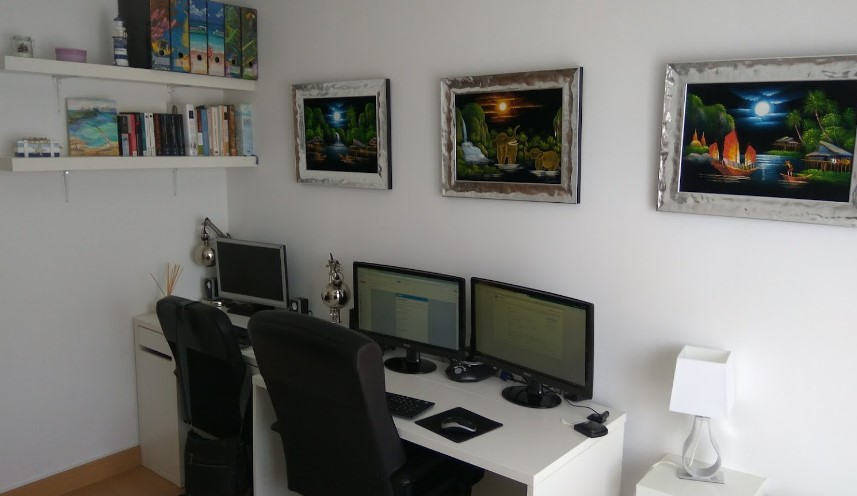
\includegraphics[width=0.8\textwidth]{./figuras/setup_cero.jpg}
\caption{Setup pre pandemia.}
\label{F:setup_cero}
\end{center}
\end{figure}

Curiosamente pocos meses antes de la pandemia, con el objetivo de cumplir la cobertura 90\% establecida por ley para 2020\cite{c_boe_fibra}, se desplegó satisfactoriamente una red de fibra en toda la zona residencial, permitiendo conectividades simétricas de hasta 300 Mbps.

Afortunadamente en mis planes familiares ya contaba con una reforma y mejora de la sala de estudio para adecuarla como dormitorio con escritorio, pudiendo usar como zona de trabajo o habitación de invitados, en perspectiva a un futuro familiar como habitación para un niño o niña.

\begin{table}[htb]
    \centering
    \caption{Setup pre pandemia tabla comparativa}
    \label{T:comp_setup_prepandemia}
    \begin{tabular}{|p{2.5cm}|p{2.5cm}|p{2.5cm}|p{2.5cm}|p{2.5cm}|}
    \hline   \hline
        ~ & \textbf{Zona de trabajo} & \textbf{Hardware} & \textbf{Red} & \textbf{Otros} \\ \hline
        \textbf{Setup} & Escritorio dedicado Sillas de estudio & 2 pantallas 21’ HD PC old-2011 laptop 2013 & Wimax 2/3Mbps Wifi g 54 Mbps & Iluminación  natural y artificial adecuadas \\ \hline
       \textbf{Defectos o planes pendientes} & Mesa baja y poco ancha & Viejo, uso hobbies & Mejora a Fibra pendiente  & Mayor capacidad de almacenaje y eliminación de 2º escritorio diminuto  \\ \hline
    \end{tabular}
\end{table}

 Desde la llegada de la fibra también realice las incorporaciones de una pizarra y una impresora 3D para mis hobbies, así como un cableado de la habitación con ethernet para obtener la máxima velocidad y no ocupar la red Wifi.

 \subsubsection{Pandemia}\label{S:setup_pandemia}
 Dos semanas antes de los reales decretos que pusieron en marcha los mecanismos de aislamiento de la pandemia, la empresa en la que trabajo me proporcionó un portátil como nuevo hardware de trabajo, las credenciales y una vpn para conectarme, comenzando inmediatamente el 100\% del trabajo en remoto como medida precautoria.
 
\begin{figure}[!htb]
\begin{center}
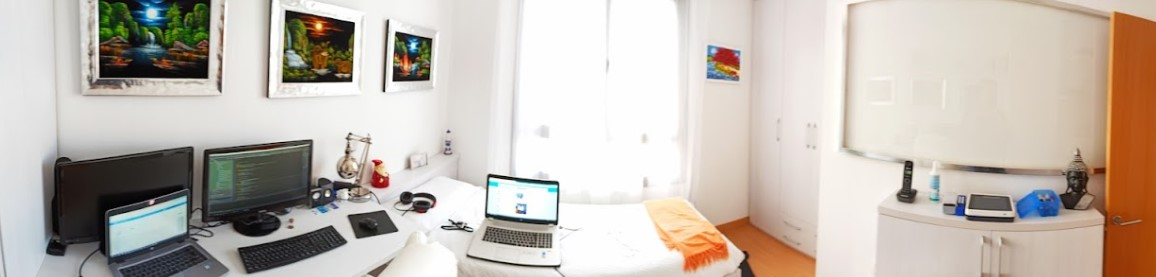
\includegraphics[width=0.95\textwidth]{./figuras/setup_uno.jpg}
\caption{Setup pandemia.}
\label{F:setup_uno}
\end{center}
\end{figure}

Los recientes cambios en la habitación de estudio me permitieron un teletrabajo satisfactorio únicamente degradado por pequeños problemas fácilmente solucionables como la adquisición de un split usb-vga para la utilización de ambos monitores con el portátil laboral, junto a la conexión de mi pc personal.

\begin{figure}[htb]
\begin{center}
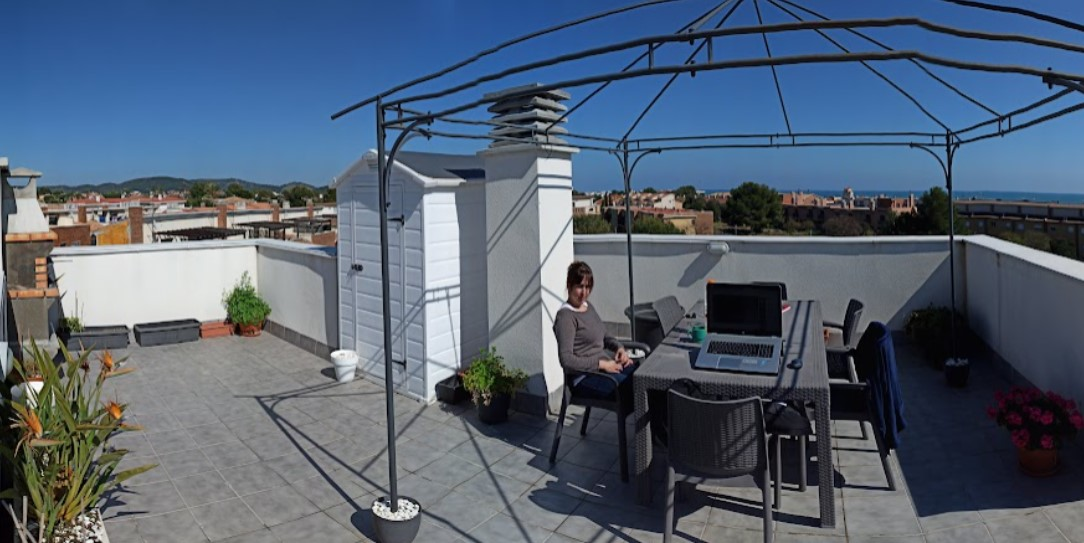
\includegraphics[width=0.9\textwidth]{./figuras/terraza_cero.jpg}
\caption{Terraza en pandemia.}
\label{F:terraza_cero}
\end{center}
\end{figure}

Una de mis tareas de bricolaje durante la pandemia fue la mejora con la instalación de cableado eléctrico para iluminación y enchufes en la terraza. Incluyendo red eléctrica en una caseta de almacenaje situada en la misma. 

\begin{table}[htb]
    \centering
    \caption{Setup Pandemia tabla comparativa}
    \label{T:comp_setup_pandemia}
    \begin{tabular}{|p{2cm}|p{3cm}|p{2.75cm}|p{2.75cm}|p{2.75cm}|}
    \hline   \hline
        ~ & \textbf{Zona de trabajo} & \textbf{Hardware} & \textbf{Red} & \textbf{Otros} \\ \hline
        \textbf{Setup incremental} & +Zona de trabajo a medida adecuada +Mesa alta (+70cm) +Mueble a medida con pc, cableados ocultos +gran capacidad organizativa y de almacenamientos +impresora 3D oculta en armario & +incorporación de split usb en pantallas +cam HD +micro-auricular HD +switch ethernet & +Fibra 300Mbps +Wifi n 150 Mbps / 5G 300 Mbps + cableado ethernet & +Pizarra translúcida +cableado interior de la casa con ethernet + impresora 3D y otros elementos \\ \hline
        \textbf{Defectos o planes pendientes} & Perfecta, pero habitación planificada invitados y futuros hijos.  & Pantallas deficientes Hardware viejo & Ethernet a 100 Mbps mejorable a giga ethernet & La climatización e infraestructuras dependen de la casa. \\ \hline
    \end{tabular}
\end{table}

Con el objetivo de poder disfrutar de horas de luz y la salida al exterior en los continuados confinamientos, instale un PLC\cite{c_plc_tech} que permitía una conectividad de 7-12 Mbps emitiendo una señal wifi en la caseta de la terraza. Permitiendo trabajar algunas horas especialmente por la tarde cuando la intensidad lumínica no deslumbraba la pantalla.

Durante el año 2020, quedó patente la funcionalidad plena de la habitación de estudio como habitación dedicada a teletrabajo, reflejando aquellos punto mejorables, sin embargo también quedó patente la infraestructura del barrio, tiene 3-4 días anuales con incidencias eléctricas cuando el calor o el frío sobrecarga la infraestructura, requiriendo de un plan “b” para dichos días.

Este periodo lo damos por concluido tras finalizar los períodos de aislamiento excepcionales en 2021 y las campañas de vacunación. El teletrabajo 100\% fue continuado como medida precautoria hasta 2023.

\subsubsection{Post pandemia}
Finalmente la mayoría de los puntos mejorables como las pantallas, uso de silla ergonómica-gamer y diversos periféricos o hub fueron subsanados.

\begin{figure}[!htb]
\begin{center}
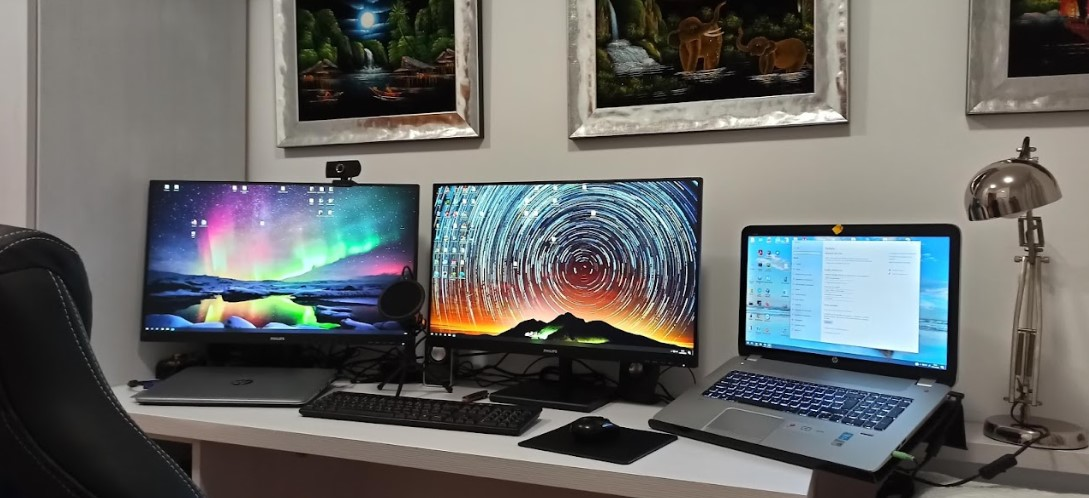
\includegraphics[width=0.85\textwidth]{./figuras/setup_dos.jpg}
\caption{Setup post pandemia.}
\label{F:setup_dos}
\end{center}
\end{figure}

Sin embargo, desde el verano de 2021, quedó patente que el principal problema era la “planificación familiar”, básicamente esa habitación estaba destinada a habitación de niño/niña con escritorio propio.
\begin{figure}[htb]
\begin{center}
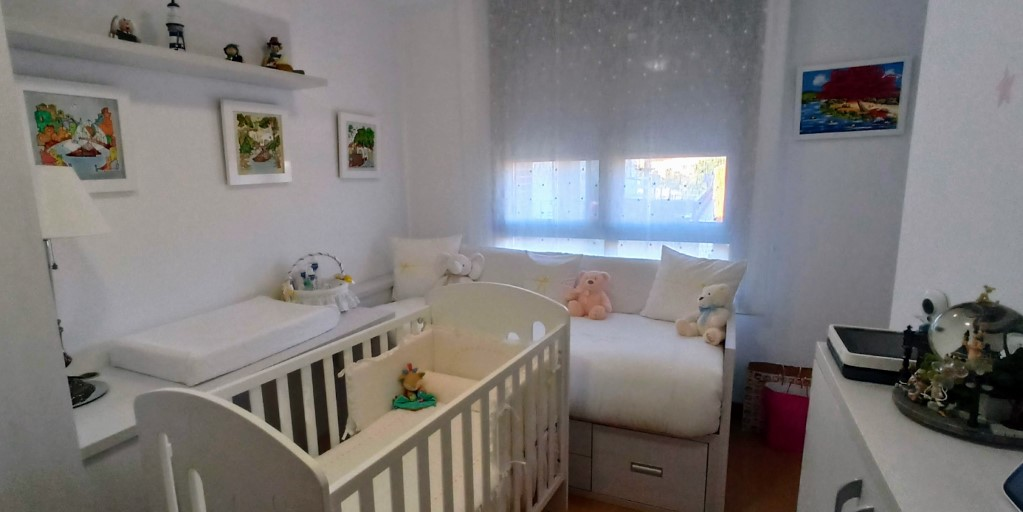
\includegraphics[width=0.85\textwidth]{./figuras/setup_bebe.jpg}
\caption{Setup 2023.}
\label{F:setup_bebe}
\end{center}
\end{figure}
El final de la pandemia reinicio los planes familiares paralizados. Como conclusión aun con la mejora sustancial del setup y sus deficiencias era necesario conseguir una alternativa real en un periodo de 12 a 18 meses incluyendo un nuevo lugar o habitáculo para el setup. Ya que a finales de 2022 el aspecto de la habitación-teletrabajo pasó a ser el siguiente:


\subsection{Nueva habitación}\label{S:nueva_room}
Vivo en un ático de 90 {\rm$m^{2}$}, desgraciadamente la disposición espacial no es eficiente ( 75 {\rm$m^{2}$} útiles) y siempre hace falta espacio de almacenamiento. La predisposición del salón o habitaciones no facilitan la instalación de una zona de trabajo, por lo que no es posible, sin dedicar una habitación en exclusiva.

En primer lugar de interés al igual que muchos amantes del bricolaje es “el trastero”, ya que unos escasos 2-6 {\rm$m^{2}$} predispuestos son más que suficientes para nuestras necesidades, sin embargo, los pisos de mi bloque no cuentan con trasteros propios, por lo que coloque una caseta de pvc en la terraza que realiza dichas funciones de almacenaje.

El segundo lugar de interés ampliamente utilizado en ciudades como Barcelona, Castelldefels o Gava, son los balcones y galerías. Espacio estrechos pero alargados fácilmente convertibles mediante cerramiento de aluminio acristalado para conseguir un espacio extra. Aunque cuento con un amplio balcón-terraza de 10 {\rm$m^{2}$}, la normativa de mi municipio no permite su cerramiento, ya que contiene una escalera de caracol que da acceso directo a la terraza superior.

Tercero, cerramiento de parking o estructura metálica sobre el parking. Dependiendo de las dimensiones acceso y altura del parking, es posible dedicar ciertos metros a una diminuta habitación mediante cerramientos simples o la instalación de estructuras metálicas con el objetivo de obtener la superficie de parking en vertical para la instalación de un trastero. La normativa comunitaria y especialmente la aseguranza de la misma no permiten la instalación de dichas estrategias ni lugares cerrados de almacenaje, por riesgo de incendio.

\begin{figure}[!htb]
\begin{center}
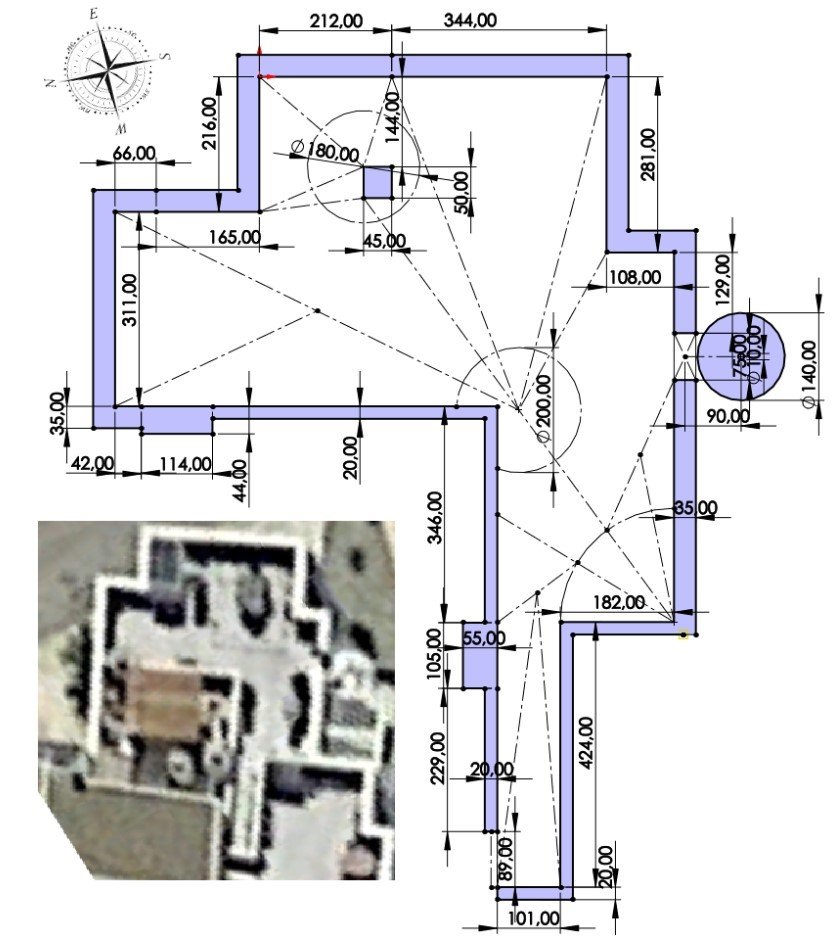
\includegraphics[width=1\textwidth]{./figuras/terraza.jpg}
\caption{Terraza planos, pendiente y zonas inúndales.}
\label{F:terraza}
\end{center}
\end{figure}

Finalmente al ser ático, dispongo de una amplia terraza, algo mayor que el 50\% de la superficie del piso (50-60 {\rm$m^{2}$}) que sin embargo, debido a su predisposición en “L”, un pasillo de acceso y una chimenea-respiradero en la parte principal más ancha, no tiene un uso práctico mayor a 35 {\rm$m^{2}$}, donde el drenaje de la misma es muy deficiente con zonas inúndales marcadas en círculos en el plano (fig.\ref{F:terraza}) que indica las pendientes de drenaje. Además es una terraza comunitaria de uso privativo, es decir, que de acuerdo a las normativa municipal y la ordenanza comunitaria, no se pueden instalar ningún tipo de elemento que:
\begin{itemize}
    \item Se fije o taladre al suelo comunitario.
    \item Rompa la estética (color) del edificio (blanco) y grises (baldosas).
    \item Medianeras, pérgolas,  mobiliario de terraza deben ser del tipo, color y dimensiones establecidas en las reglas comunitarias.
    \item Deben ser elementos de carácter no fijo (desmontables), barbacoas, barras, armarios o cerramientos únicamente anclados en paredes o alféizares.
\end{itemize}

Como especial interés, se definieron las separaciones de medianil, por paneles de aluminio lacado blanco, fuertemente anclados en los muros. Permitiendo cubrir muros vecinales o espacios entre paredes y chimeneas, siempre y cuando hubiese consentimiento mutuo entre vecinos y no se anclaje nada en fachada o paredes comunitarias.

\subsection{Caseta Oficina}
A veces las soluciones son una combinación de casuística y defectos utilizados a tu favor. Durante la pandemia intentamos solucionar los problemas de la terraza, falta de privacidad, una gran cantidad de espacio infra usado y las continuas inundaciones de la caseta-pvc usada como trastero. Así mismo la instalación del PLC y el “trabajo desde exterior” me dejó claro que con el cerramiento adecuado, era el lugar perfecto para trabajar.

\begin{figure}[!htb]
\begin{center}
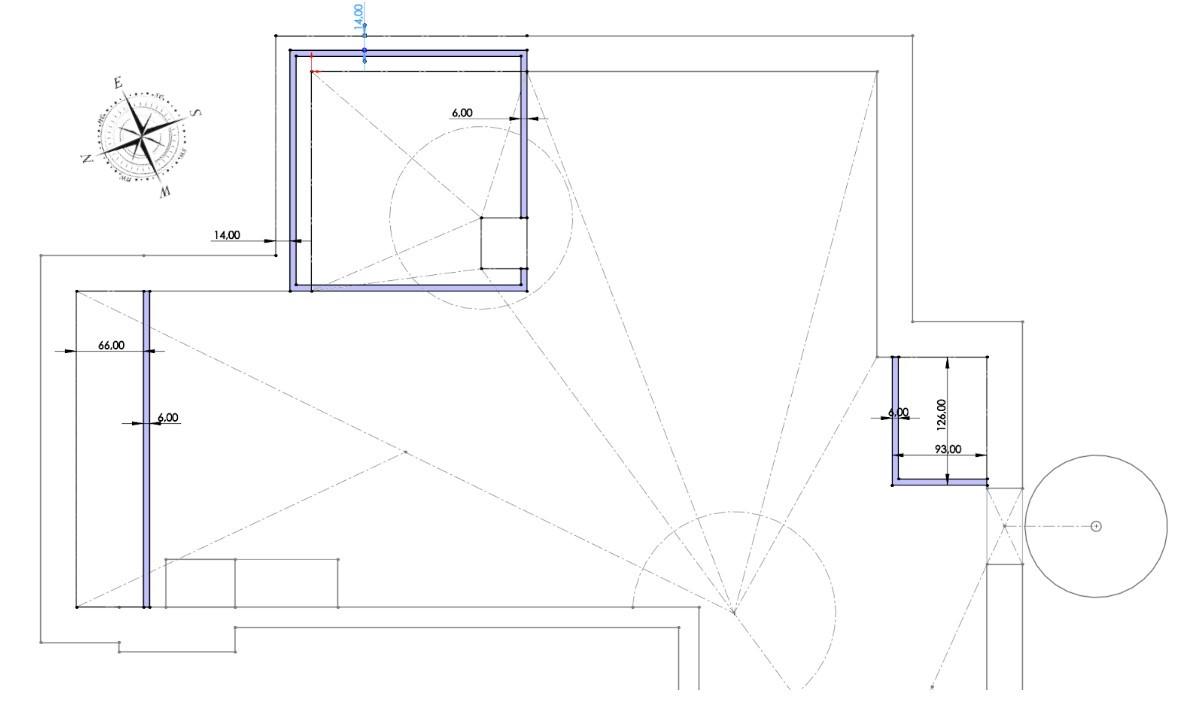
\includegraphics[width=1\textwidth]{./figuras/cerramiento.jpg}
\caption{Terraza cerramientos planificados  con pendientes zonas inúndales marcadas.}
\label{F:cerramiento}
\end{center}
\end{figure}

El plan se basaba en cerrar el medianil con el separador de aluminio para ganar privacidad y que el mismo proveedor de aluminio nos hiciera un armario-almacenaje en torno a la zona no inúndable de espacio muerto entre barbacoa y pared norte. Sin embargo no se llegó a entendimiento con el vecino. 

\begin{figure}[!htb]
\begin{center}
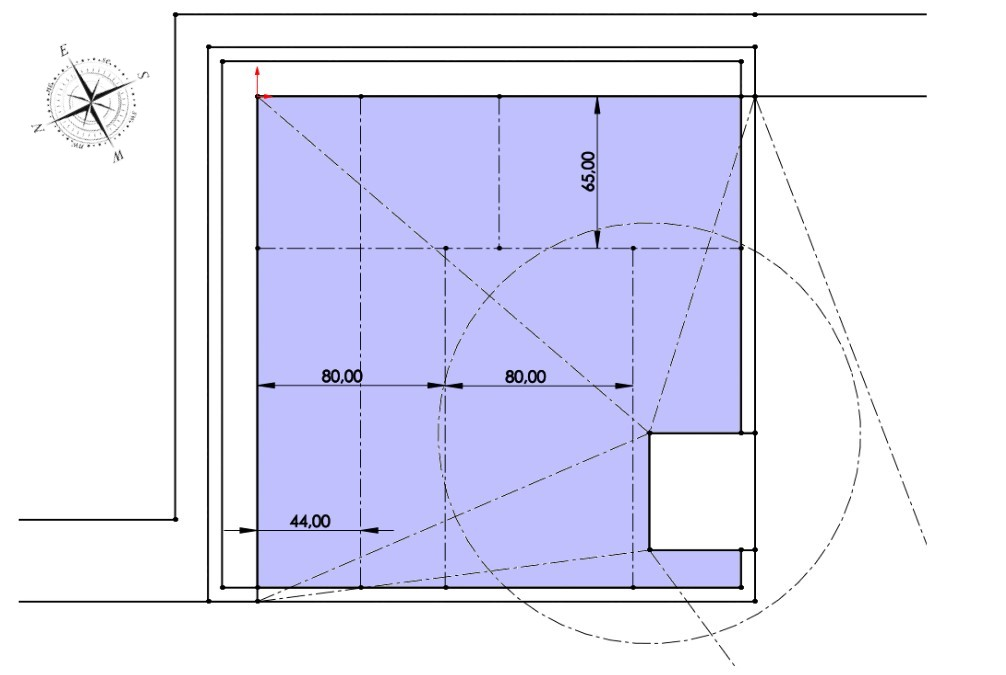
\includegraphics[width=0.85\textwidth]{./figuras/caseta_division_spacio.jpg}
\caption{Caseta división espacial.}
\label{F:caseta_division_spacio}
\end{center}
\end{figure}
Entonces comente la idea de similar al armario, rehacer la caseta-trastero de PVC, pero utilizando el material de separación entre vecinos. El objetivo inicial era conseguir una caseta hermética, evitando “el charco” y el moho, pero sobre todo ganando el alféizar como espacio útil y permitiendo colocar estantes en él, con el fin de obtener un pseudo trastero.

Al detallar, descubrimos que lo que normalmente es 1.80 m de altura, debido a la mala colocación de terraza y a un alféizar algo elevado, los puntos de anclaje de la futura caseta permitían unos valores de 1.86-1.89 m respecto al suelo real de la terraza, es decir, un lugar donde a mi altura 1.79, permite moverse como en una habitación de techos bajos. 

Por otra parte la chimenea-respiradero, pasa de ser un elemento problemático, a un elemento estructural, que permite anclar y dar robustez al formar un cuadrado entre muro-alféizar y chimenea, permitiendo el anclaje lateral y en conclusión resistir cualquier tipo de vientos al cerramiento de aluminio. Por otra parte interiormente habilita un pared robusta sobre la  que anclar elementos como pizarra o mini estanterías.

\subsubsection{Trabajos previos}\label{S:trabajos_previos}
Durante los meses previos a la instalación de la caseta se realizó una limpieza completa de las zonas afectadas. La limpieza de alféizar, pared y suelo con agua a presión, posteriormente con bases ácidas vinagre blanco (alféizar) y salfuman (baldosas) para la eliminación y apertura de poros.

\begin{figure}[!htb]
\begin{center}
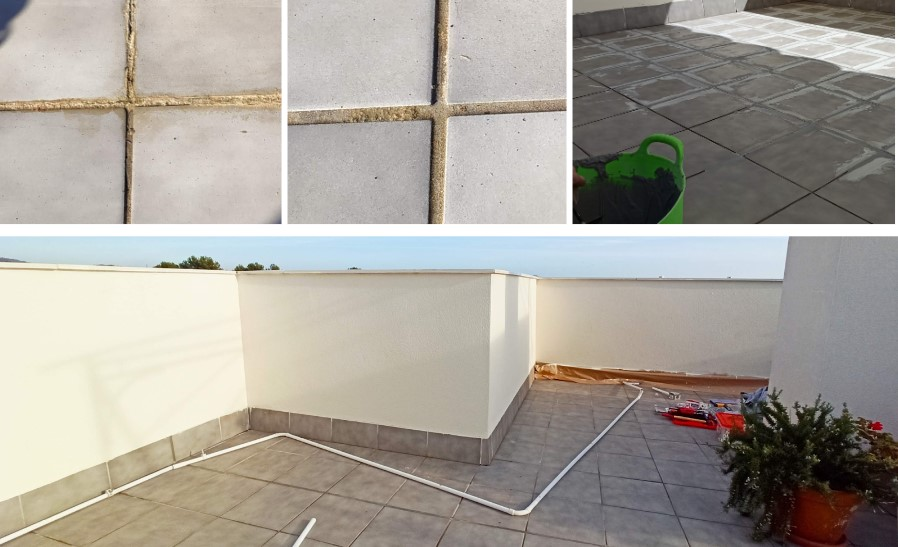
\includegraphics[width=1\textwidth]{./figuras/trabajos_previos.jpg}
\caption{Limpieza, pintura y trabajos previos.}
\label{F:trabajos_previos}
\end{center}
\end{figure}

Así como una adecuación de la instalación eléctrica con la instalación de canalizaciones, cableado y respectivas cajas con el fin de mejorar y separar completamente iluminación de terraza, enchufes húmedos, electricidad de la oficina y cable ethernet.

\begin{figure}[!htb]
\begin{center}
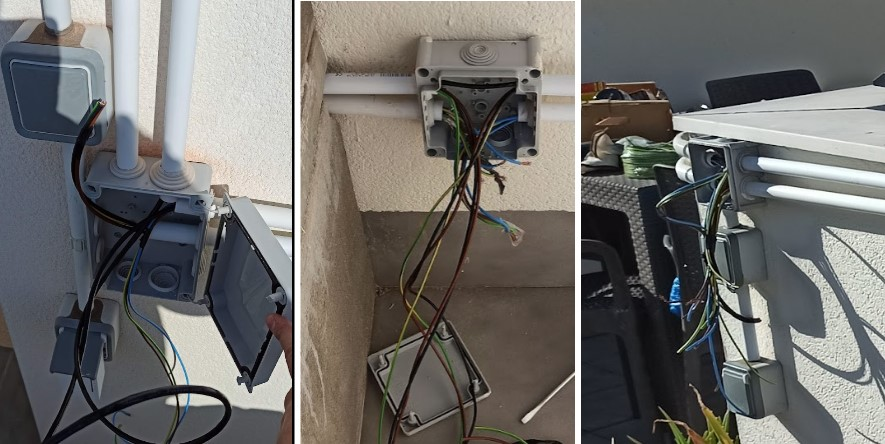
\includegraphics[width=1\textwidth]{./figuras/trabajo_electrico.jpg}
\caption{Montaje de sistema eléctrico y cableado Ethernet.}
\label{F:trabajo_electrico}
\end{center}
\end{figure}

\subsubsection{Estructura, aislamiento y estanqueidad} \label{S:estructura_aislamiento}
La estructura y el aislamiento viene de la mano de paneles sándwich de aluminio, al igual que la separación entre vecinos se basan en anclajes verticales, que unen los paneles de aluminio cada 1.5-2 metros. 
\begin{figure}[!h]
\begin{center}
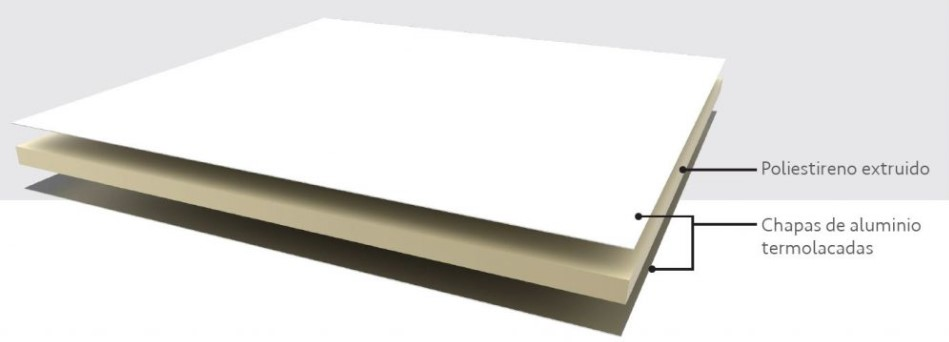
\includegraphics[width=1\textwidth]{./figuras/panel_aluminio.jpg}
\caption{Panel de aluminio lacado con aislante térmico.}
\label{F:panel_aluminio}
\end{center}
\end{figure}
\begin{figure}[!h]
\centering
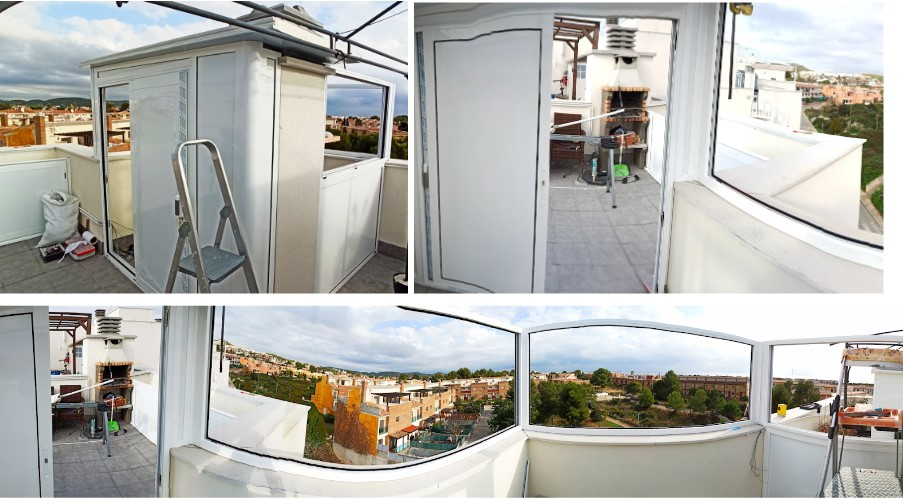
\includegraphics[width=1\textwidth]{./figuras/montaje_aluminio.jpg}
\caption{Montaje paneles aluminio y soportes.}
\label{F:montaje_aluminio}
\end{figure}
\begin{figure}[!h]
\centering
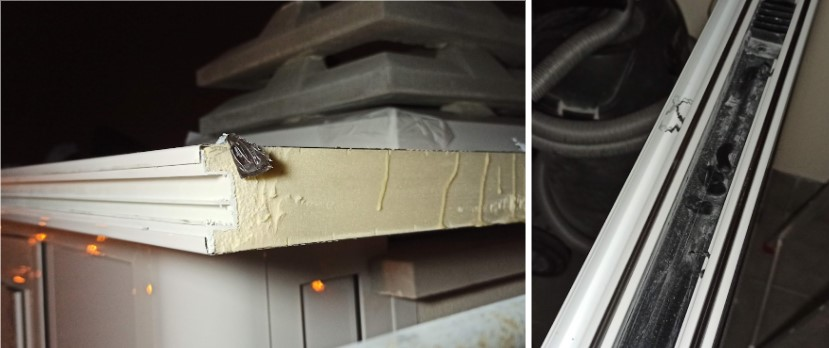
\includegraphics[width=1\textwidth]{./figuras/perfil_aislamiento.jpg}
\caption{Vista de perfiles y techo con aislamiento.}
\label{F:perfil_aislamiento}

\end{figure}
La estrategia se basa en utilizar paneles más grueso de 4 cm para un mayor aislamiento, especialmente en tejado 7 cm, ya que la incidencia solar es directa y prolongada durante los meses de verano. Estos paneles, son sujetados por premarcos de aluminio (similares a ventanas) que a su vez se fijan directamente sobre alféizar, paredes o perfiles estructurales en las esquinas. 
Todos ellos entre sí, así como los elementos que se fijan quedan perfectamente sellados por siliconas especializadas, incluido la base del perfil en contacto con el suelo de la terraza.

\subsubsection{Instalación interna y montaje mobiliario}
Una vez terminados los trabajos de instalación de los cerramientos y el apropiado secado de los mismo, se inició un montaje tanto de cajas, enchufes e interruptores eléctricos de ambos cerramientos
\begin{figure}[!htb]
\begin{center}
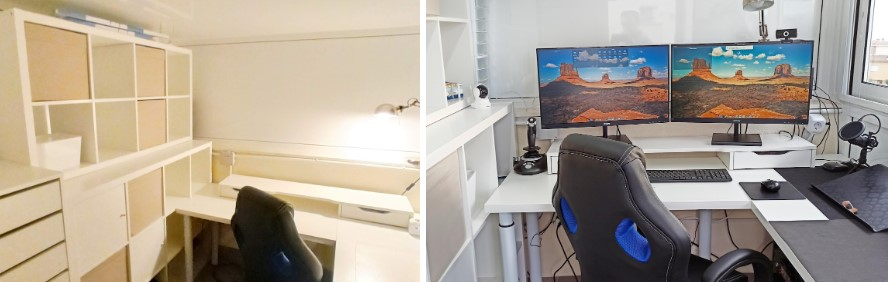
\includegraphics[width=1\textwidth]{./figuras/caseta_mobiliarioysetup.jpg}
\caption{Mobiliario y setup en caseta.}
\label{F:caseta_mobiliarioysetup}
\end{center}
\end{figure}
Junto con una migración del setup validando tanto conectividad, enchufes e iluminación, permitiendo comenzar el teletrabajo desde la oficina conforme se van añadiendo más elementos complementarios necesarios especialmente relacionados con temperatura e iluminación.
\begin{figure}[!htb]
\begin{center}
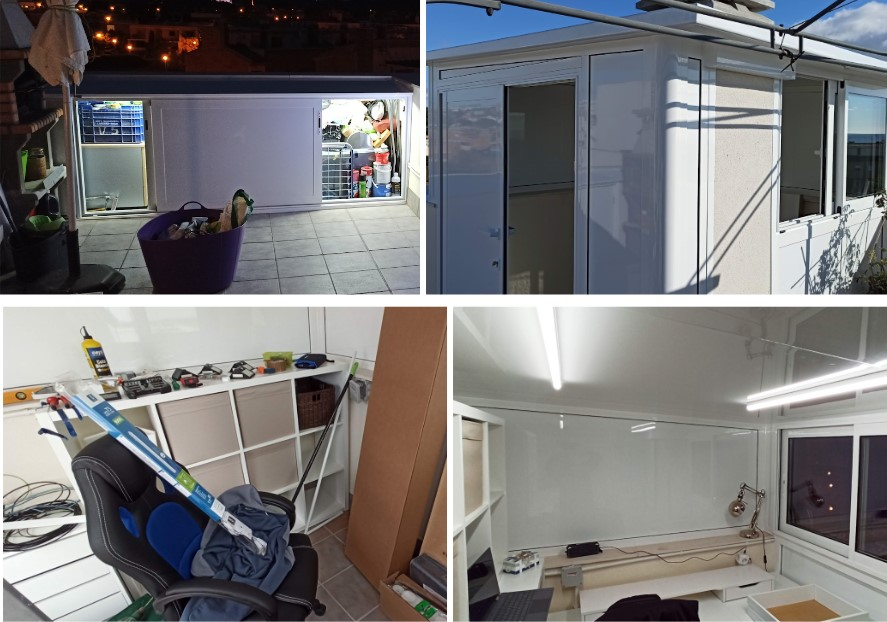
\includegraphics[width=1\textwidth]{./figuras/caseta_electricidad.jpg}
\caption{Instalación eléctrica en caseta y cerramientos.}
\label{F:caseta_electricidad}
\end{center}
\end{figure}

\newpage
\subsubsection{Aclimatación e iluminación}\label{S:iluminacion_caseta}
El primer elemento necesario de la “hermética caseta” es la instalación de varios respiraderos naturales para la circulación de aire, siendo estos fácilmente operados manualmente para evitar la entrada de frío/calor en circunstancias adversas.

 Aunque el aislamiento bastante sobredimensionado para un cerramiento usual, no deja de ser 4-7 cm similar a una puerta de parking, es decir, bastante útil para evitar el calor directo pero insuficiente en invierno para evitar la bajada de temperaturas. Por otra parte tanto el muro como el suelo original son elementos fríos, que permanecen a la temperatura de la estructura del edificio, algo fresca en verano pero fría en invierno.

 Por lo tanto se han instalado alfombras (duras y gruesas) junto a un calefactor eléctrico, así como ventiladores pingüino de bomba de calor aire frío/calor.

 \begin{figure}[!htb]
\begin{center}
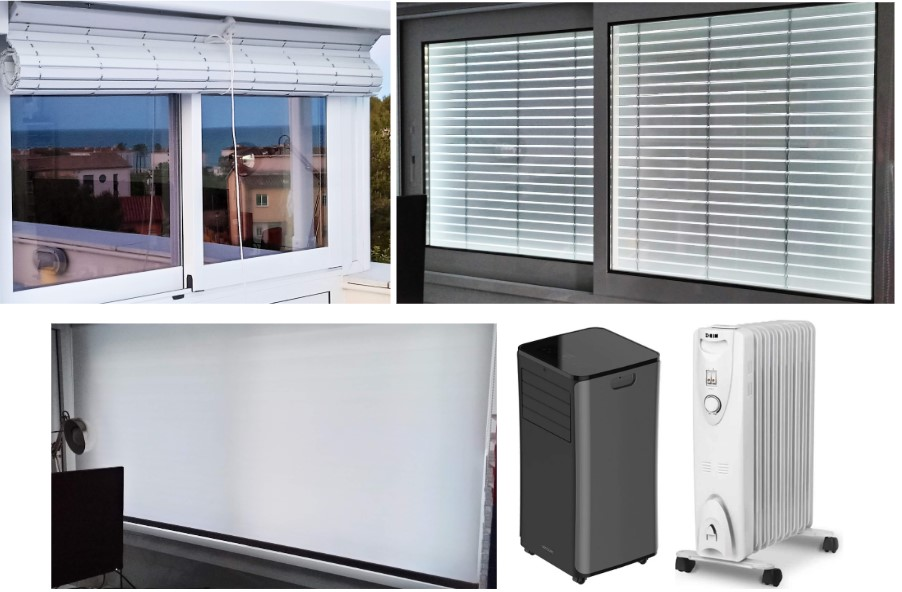
\includegraphics[width=1\textwidth]{./figuras/luz_regulacion_termica.jpg}
\caption{Regulación térmica y lumínica.}
\label{F:luz_regulacion_termica}
\end{center}
\end{figure}

Finalmente la ventana se ha utilizado un cristal especial, que minimiza la entrada de calor por vía solar, especialmente intensa en verano, que a su vez debido también al fuerte reflejo directo continuado por la vista directa al mar, ha obligados a la colocación tanto de un estor difusor de luz, así como una alicantina externa con el objetivo de reducir sustancialmente la intensidad y la dirección lumínica de la luz natural.

\subsection{Mejoras de Terraza}
A continuación se han realizado varias mejoras a la terraza que aunque no tiene conexión directa con la “oficina-caseta” influyen positivamente en la misma.

\begin{figure}[!htb]
\begin{center}
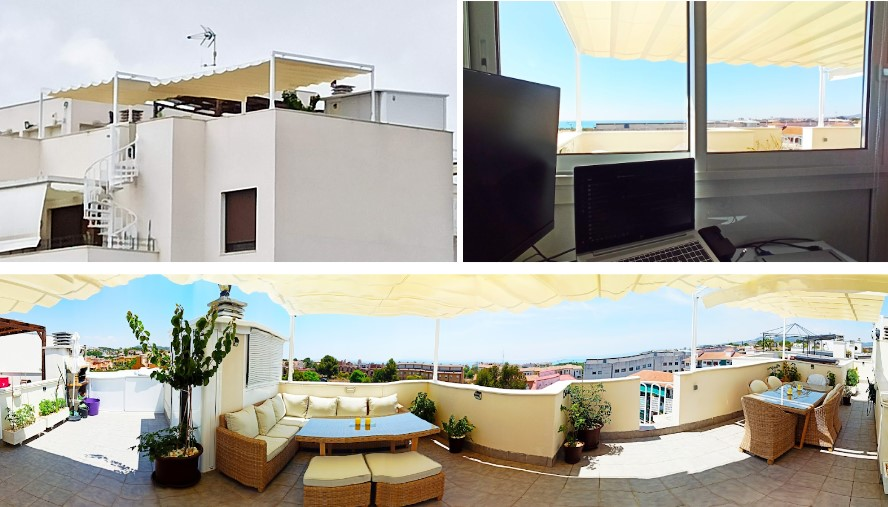
\includegraphics[width=1\textwidth]{./figuras/mejoras_terraza.jpg}
\caption{Mejoras externas de terraza que afectan a la caseta.}
\label{F:mejoras_terraza}
\end{center}
\end{figure}
Una de las grandes desventajas de la terraza es su nulo uso entre junio-septiembre debido a la alta intensidad lumínica y de calor, debido al número de horas de luz directa más el reflejo del mar. Con el objetivo de mejorar su uso, así como reducir la temperatura del suelo y reducir el calor que transmite al ático, se implementado dos toldos corredero de grandes dimensiones, que junto a una vela triangular y una sombrilla, permiten cubrir el 80\% de la terraza en sombra las principales horas del dia 11-17, así como provocan una zona en sombra tanto a la paredes de la caseta como parcialmente en el tejado de la misma.

\begin{figure}[!htb]
\begin{center}
\includegraphics[width=1\textwidth]{./figuras/mejoras_terraza_2.jpg}
\caption{Mejoras externas de terraza II que afectan a la caseta.}
\label{F:mejoras_terraza_2}
\end{center}
\end{figure}

Por otra parte se ha renovado el mobiliario exterior, la distribución del mismo, permitiendo salir al exterior de manera cómoda cuando las condiciones climáticas y lumínicas lo permiten.

\section{Evaluaciones, mejoras y correcciones}\label{S:cambios_2023}
Por otra parte se han detectado mejoras realizadas sobre el diseño original así como estrategias fallidas durante 2022-23 que han requerido de arreglos o un cambio radical en la solución final.

\subsection{Humedades y condensación}
Aunque el hermetismo del cerramiento es perfecto existen dos fuentes de humedades resueltas parcialmente. 

La principal son el alféizar y muros originales del propia cerramiento, aunque están debidamente pintados con pintura transparente anti-humedad, esta capa únicamente limita la salida o la evaporación de la humedad, permitiendo que aquellas semanas con 3-6 días de lluvias continuadas la humedad progrese por la pared hasta llegar al zócalo por donde aparece en forma de superficie húmeda.

Las juntas entre las baldosas, como se ha explicado el cerramiento se sitúa sobre un punto más bajo que el resto de la terraza, esto junto a la porosidad tanto de baldosas como de juntas, promueve un lento avance de humedades los días de lluvia,y de igual manera cuando supera los 2-3 días comienza no solo a “humedecer” sino a acumular 1-3 mm de agua.

\begin{figure}[!htb]
\begin{center}
\includegraphics[width=1\textwidth]{./figuras/humedades.jpg}
\caption{Impermeabilización con pintura y silicona.}
\label{F:humedades}
\end{center}
\end{figure}

La solución de ambos problemas ha sido múltiples capas de pintura anti-humedad junto a el uso de silicona líquida para sellar completamente tanto suelos como zócalos o posibles entradas de agua por porosidad o capilaridad.

Otro problema recurrente es el propio hermetismo de la sala, si se cierran los orificios de ventilación en invierno con la finalidad de mantener la temperatura. Cualquier humedad interna, especialmente el propio vapor humano, termina condensando en los paneles de aluminio o ventanas, cuya única solución es ventilar intervalos de 3-5 horas, con especial interés previos a la noche.

\subsection{Bomba de calor/frío}\label{S:cambios_bombacalor}
El uso del “pingüino” para calentar, enfriar o des humidificar ha sido un completo fracaso. Aunque la potencia del mismo es para habitaciones de 15 {\rm$m^{2}$} (ampliamente sobredimensionado), el caudal de aire entrante-saliente necesario para su funcionamiento hace ineficaz su uso debido a las pequeñas dimensiones de la habitación.

Enfría / calienta un aire que se renueva rápidamente 10-20\%, es decir, que gran parte del movimiento térmico realizado, se utiliza para re-aclimatar el aire nuevo, no permitiendo subir de los 21º en invierno (12-17º exterior), o bajar de 24º en verano (28-33º exterior), a su vez esta renovación de aire trae consigo humedad que el sistema debe retirar, es decir está continuamente eliminando humedad, que debido a al mal drenaje de la terraza se convierte en un charco o un recipiente a vaciar manualmente.

La reducción u obstrucción de la ventilación para reducir el caudal de aire exterior soluciona parcialmente el problema pero convierte la pequeña y hermética caseta, en una sala de presión negativa, sobre esfuerza el motor que expulsa el aire, estresa la estructura de aluminio y genera “silbidos”  por la presión negativa en la puerta corredera. 

Por último su mayor problema es que su uso continuado genera excesivo ruido tanto para vídeo conferencias, dificultando la concentración e incluso generando dolor de cabeza. La humedad es un problema especialmente dañino en verano puesto que aunque la temperatura generada dura 90-120 minutos debido al aislamiento, la humedad se re-equilibra con el exterior rápidamente en cuestión de 15 minutos.

Finalmente la realidad ha sido que la desmantelación total de la bomba de calor y el uso de elementos más rudimentarios tales como un calefactor eléctrico tradicional o el uso de la brisa veraniega combinada con ventiladores, satisfacen de una manera más adecuada y sin problemas (ni el gasto eléctrico sobredimensionado).

\subsection{Paneles solares y SAI}
La desaparición de la bomba de calor portátil ha proporcionado un espacio debajo de la mesa útil para la generación de un SAI casero, véase figura \ref{F:instalacion_electrica} donde se predispone la batería y generador de alterna contiguo a un conjunto de enchufes. 

Con el objetivo de disponer de una fuente de energía alternativo para el setup, así como permitir la alimentación tanto de ventiladores, calefactores eléctricos o servidores autocráticos se ha instalado una batería solar de 128 AH a 12 V de ciclos profundo junto con la instalación de paneles solares que alimentan el sistema.

\begin{figure}[!htb]
\begin{center}
\includegraphics[width=1\textwidth]{./figuras/panel_solar.jpg}
\caption{Paneles solares, tejado y frontal chimenea.}
\label{F:panel_solar}
\end{center}
\end{figure}

Se ha predispuesto de un panel solar de 160 W orientado a  sur en el tejado, cuya eficiencia se ve lastrada por la inclinación del mismo (5º), pero permite una captación de luz permanente durante el 80\% de las horas diurnas, así como el reflejo y dispersión atmosférico. Permite captar 0.5-2 A durante las horas mínimas(6-24w), 6-7A al medio día en invierno y 10-11 A en verano, es decir, entorno 80-130W. Así mismo con el objetivo de compensar la  horizontal y el cambio de posición solar invierno/verano se ha instalado un panel de 100W de alta eficiencia en paralelo en orientación sur vertical, que aparte de la luz directa, recibe de manera constante y directa el reflejo marino durante todo el día.

La conjunción de ambos paneles generan un flujo constante y complementario de corriente, compensando tanto la inclinación solar durante las estaciones, como su transito durante el día. Buscando un suministro constante de 30-50W en las peores condiciones y picos de productividad 150-170W durante el medio día soleado.

La principal función de este sistema es un uso constante de los sistemas ambientales, ventiladores en verano (5w, 5w, 25-50w), el uso de calefactores en invierno 150 w, así como el almacenaje de la energía no utilizada para la funcionalidad de SAI, proporcionada por un generador continua-alterna de 1000W, fácilmente conmutable para alimentar pantallas y laptop en periodo de 4-6 horas.

\subsection{Domótica y alarma}
Durante 2023 he implementado diversos mecanismo de domótica y seguridad en mi vivienda. Entre ellos la instalación de:
\begin{itemize}
    \item Sensores de presencia, sensores magnéticos (puertas, ventanas), sensor de humo/gas, sensor temperatura / humedad, detectores de presencia  y termostato inteligente.
    \item Alarma con batería y conexión 3G / wifi, usando aplicación genérica de domótica y API de eventos.
    \item Actuadores tales como bombillas inteligentes, enchufes inteligentes, regletas y conmutadores inteligentes, PIA inteligente, diferencia rearmable.
    \item Interfaces humanas, smart tv, amazon alexa, google eco.
    \item Gateways de zigbee, z-wave, wifi, bluetooth y 144 Mhz.
    \item Cámaras Ip fijas, o con actuadores.
    \item Rasberry pi con home assitand y API configuradas (google, alexa y gautone).
\end{itemize}

Aunque son elementos asociados a la vivienda y automatizados en mis cuentas personales, afectan a la oficina automatizado el encendido y apagado de elementos tales como climatización, monitorizando terraza o interior de caseta (cámaras y sensores de temperatura y humedad) así como proveen una seguridad y notificación efectiva del área de trabajo.

\chapter{Software y Nube}\label{S:anexo_C}
Este anexo muestra el razonamiento detenido, la comparativa de pruebas de concepto realizadas en el anexo \ref{S:anexo_E} y configuración dentro del capitulo 2.

\section{Software}\label{S:decisiones_software}
El primer punto que debemos decidir\cite{c_inhouse_outsource} es la modalidad del tipo de servicios que queremos utilizar. Desde el punto de vista técnico, podemos optar entre la externalización o la autogestión, y llegado a un extremo la nube autócrata. Por otra parte, la licencia del software a utilizar así como la flexibilidad, customización y costes asociados difieren entre dos tipos de soluciones “la solución completa” dentro de un marco de trabajo (usualmente privado y de pago) o “soluciones concretas” que se integran con diferentes gestores y se basan comunidades auto documentadas (generalmente más económica y libre). 

\subsection{Proveedor, mantenimiento y gestión}
Externalizar significa utilizar un servicio público proveído por empresas ya sea en modalidad gratuita o de pago. Al ser un producto estándar conlleva ventajas y desventajas, no es customizable, pero facilita su uso y mantenimiento, siendo normalmente transparente al usuario. 

Auto gestionar sin embargo indica que aunque sea un producto estándar, la instalación, mantenimiento y solución de incidencias es propia. Requiere de un mayor conocimiento técnico y una dedicación semanal o mensual para tareas de mantenimiento o prevención, sin embargo además de una mayor customización y agilidad con las incidencias, usualmente es mucho más económico en términos generales.

La externalización se puede producir a diferentes niveles, la autogestión usualmente externaliza el hardware/servidor o la gestión de la máquina virtual pero mantiene y gestiona el software instalado. Un usuario puede decidir usar su propio hardware y su conexión a internet para generar una nube autócrata, pero cuya complejidad y mantenimiento a veces no la hace funcional, simplemente autócrata y debido al coste eléctrico asociado lo hace inviable económicamente hablando.

Finalmente se debe entender que a veces un software funciona como un servicio. Gestionar un servicio muchas veces no tiene que ver con el propio software sino con la escalabilidad, backups y transferencia del servicio a otro proveedor, por lo que la autogestión y \textbf{la externalización parcial deben ser fácilmente intercambiables}.

\subsection{Licencias y tipo de software}
Por otra parte, hay que decidir qué aplicativo usamos entre las múltiples posibilidades que ofrecen un resultado similar, pero cuyas características legales y técnicas cambian. 

Existen 5 propiedades intrínsecas a todo software:
\begin{itemize}
    \item Propiedad intelectual.
    \item Tipo de licencia de uso, distribución y/o modificación.
    \item Código abierto (publicado) o cerrado.
    \item Compatibilidad, requisitos o ecosistema integrado.
    \item Vida útil, refiere al mantenimiento, LTS, actualización del software. 
\end{itemize}

\begin{figure}[!htb]
\begin{center}
\includegraphics[width=0.9\textwidth]{./figuras/licencias.jpg}
\caption{Tipos de licencias mas comunes\cite{c_licencias}.}
\label{F:licencias}
\end{center}
\end{figure}

Obviando la casuística concreta de cada software, en una visión global se pueden distinguir dos bloques claros de tipos de software:

“Software privativo”, son aquellos cuyo propietario es una persona o empresa y el uso de dicho software requiere de licencia gratuita o de pago. Así como los requisitos del mismo depende de la compatibilidad realizada por el propietario.
Desde el punto de vista técnico, estos software pueden ser abiertos o cerrados indicando si el código que los construye es público/visible o no. Usualmente estos softwares son de pago, o licencias gratuitas bajo restricciones y suelen funcionar bajo entornos de trabajo privativos que unifican un conjunto de aplicaciones como solución interdisciplinar. Ejemplo entorno de trabajo Microsoft (azure, windows, office, github, atlassian solutions), entornos de trabajo Google(cloud, chromium OS, gmail, maps ...) .

“Software Libre”, es un término que hace referencia a la libertad para usarlo, estudiarlo, distribuirlo, adaptarlo o mejorar el programa. Estos software pueden ser tanto empresariales como realizados por comunidades o programadores independientes, en todos los casos los creadores del software siguen siendo sus propietarios, pero no existe restricciones a su uso o mejora, así como tienen licencias de coste cero. La principal ventajas de estos software son las comunidades y la facilidad de mejora del código al ser abierto. Por otra parte las empresas que colaboran o sustentan estas aplicaciones, ofrecen dichos software a precios competitivos, donde el coste está asociado a la infraestructura, gestión y mantenimiento del software no a la licencia en sí y normalmente permiten la existencia de un mercado de plugins, módulos o configuraciones extras proveídas tanto por empresas como programadores profesionales. Ejemplos: linux, libreoffice y aplicaciones web o frameworks (ubuntu, wordpress, prestashop, frameworks como laravel, angular, spring boot).

Actualmente existe una mayor popularidad de software libre en servidores, aunque por contra posición el mercado es mayoritariamente privativo en el segmento escritorio. Esto se debe especialmente al SO (Sistema Operativo) empleado en las diferentes plataformas que condicionan los ecosistemas utilizados.

\section{Elección de Servidor}\label{S:anexo_segurizacion}
El primer elemento necesario de nuestra cloud, es el servidor principal. Debido a que nuestro objetivo primario es la instalación de múltiples softwares y la gestión de los mismos, lo más intuitivo es el uso de un servidor o VPS (virtual private server) sin embargo otras opciones como la dockerización de servicios directamente por un proveedor también es una opción valida.

\subsection{Servidor Físico vs Servidor virtual vs Cloud Externo}
Existen dos opciones basadas en servidores físicos, la principal es la contratación a un proveedor de una máquina con características específicas; usualmente este tipo de servidores son de un coste alto y unos requisitos de hardware excesivos para nuestras necesidades. La secundaria el uso de VPS o servidores virtuales dinámicos no sólo permite reducir significativamente su coste, sino que también está asociados a un escalado dinámico (vertical) más flexible y en función de la demanda.

\begin{figure}[!htb]
\begin{center}
\includegraphics[width=1\textwidth]{./figuras/servidores_typos_servicios.jpg}
\caption{Tipos de servicios en servidores\cite{i_vps}.}
\label{F:servidores_typos_servicios}
\end{center}
\end{figure}

La alternativa es el uso de un servidor propio instalado, en la “oficina real”. Obviando el hecho de la compra del hardware o el reuso de un pc para dichos fines, requiere de una conexión a internet alta velocidad y simétrica (fibra) y un consumo eléctrico continuado. Dependiendo del ISP(Internet Service Provider), existirá un problema de IP dinámica, puerto dinámico o servicio de pago para la obtención de IP estática, incluso la no existencia de una ip pública por CG-Nat\cite{c_cg_nat}.

\begin{table}[!ht]
    \centering
    \label{T:tipos_servidores}
    \caption{Tabla comparativa opciones servidor.}    
    \begin{tabular}{|p{3cm}|p{3.5cm}|p{3.5cm}|p{3cm}|}
    \hline \hline
        \textbf{Tipo de solución} & \textbf{Ventajas} & \textbf{Desventajas} & \textbf{Coste} \\ \hline
        Virtual Private server (bajos recursos) & Externalizado, alta disponibilidad, escalabilidad y migración & Servicios de backup costoso. Recursos limitados & 3-15 € / mes \\ \hline
        Dedicated Server & Zero problemas técnicos & Coste alto, menos flexible a escalar que VPS & 25-300 € / mes \\ \hline
        Office Server (pc antiguo, ip dinámica) & Autócrata, uso de ddns para la IP gratuitos. Reciclado Hardware & Disponibilidad no asegurada. & 40-70 € / mes (coste eléctrico) 10-20€ / mes (ddns profesional) \\ \hline
        Office Server, de bajo consumo (Raspberry pi, nuc) IP dinámica & Autócrata Uso de ddns para la IP gratuitos & Disponibilidad no asegurada. Recursos limitados Especialmente CPU & 5-20 € / mes (coste eléctrico) 10-20€ / mes (ddns profesional), compra hardware \\ \hline
        Office Server puerto dinámico & Autócrata & Requieren de conexión inversa a través de un enlace exterior Disponibilidad no asegurada. & 5-30 € / mes (coste eléctrico) \\ \hline
        Office Server IP estática & Autócrata & Ip estática excesivamente cara. Disponibilidad no asegurada. & 5-30 € / mes (coste eléctrico) 30-60 € / mes (IP estática) \\ \hline
    \end{tabular}
\end{table}

Analizando los costes de cada una de las posibles opciones tabla \ref{T:tipos_servidores} se concluye en todos los casos en soluciones \textbf{no profesionales} o \textbf{el coste no es proporcional al servicio obtenido}. Por lo tanto las opciones más económica, aceptable y elegida es \textbf{VPS} con unos recursos asegurados o la contratación de ejecución de contenedores en un cloud. Esta elección facilita un despliegue 'low cost' pero condicionara diferentes elecciones durante todo este documento buscando un uso bajo de recursos.

La contratación de containers en una nube, usualmente es proveída por Amazon, Google permiten un uso de recursos basado en escalado, es decir, un pago por uso. Aunque puede ser muy interesante como plataforma base para desplegar un producto que requiere escalar, \textbf{no son los proveedores más económicos} para un uso constante y estático de recursos. Por ello el uso de '\textbf{VPS low cost'} permite obtener un servidor base en precios de \textbf{3-5€ / mes} que pueden compaginarse con escalados, migraciones o el uso en paralelo de las nubes de contenedores para aquellos servicios o productos que sí lo requieran.

En este caso \textbf{se ha seleccionado OVH\cite{c_vps_ovh} o time4vps\cite{c_vps_time4vps} como proveedores}, debido a su gran competitividad en recursos / precio, por los descuentos especiales que se pueden conseguir y ser un proveedor europeo con varias posibles sedes que \textbf{cumplen nuestros requisitos legales como proveedor bajo la legislación europea}\cite{c_ue_rpgd}.

\subsection{Securización}
La seguridad preventiva externa se obtiene exponiendo únicamente el servicio SSH interno del servidor (apropiadamente securizado) y los servicios dockerizados públicos, negando o reaccionando con baneación de IP (black list) a la gran mayoría de ataques reincidentes denegados.

La seguridad preventiva interna se basa en limitar el acceso y traceado. Durante la instalación de docker se subscribe el servicio a un grupo ‘docker’ guid 997, con el fin de centralizar los permisos del servicio como el sistema de archivos de los volúmenes a utilizar. El acceso, cambio y ejecuciones tanto de ‘sudo’ como ‘docker’ y ‘docker-compose’ pueden ser auditados con logs y notificaciones de las acciones. Y especialmente gestionando y evitando el colapso de recursos como disco, ram o cpu con las estrategias pertinentes.

Finalmente solo el administrador de sistema debe tener acceso directo puesto que el resto de acciones referente a software pueden realizarse mediante ansible ejecutado previamente por in CI/CD o scripts automatizados lanzados por eventos de cron.

La utilización de \textbf{redes internas docker}\cite{c_docker_network} donde suscribir aquellos servicios dockerizados no expuestos directamente, y el uso de vpn-intranets, conectado a estas redes internas permite un acceso directo a los servicios, o una red puente por la que acceder a otros servidores o granjas interconectados.

La implementación de un servicio SSO \cite{c_sso}(single sign on) o LDAP\cite{c_ldap}(Lightweight Directory Access Protocol) como autenticación centralizada de usuarios debe evaluarse si la empresa supera los 10 trabajadores(véase anexo \ref{S:sso_example} ejemplo), o las rotaciones de personal son altas, pero no son prácticos o conllevan un coste excesivo para nube personales.

\subsection{Setup y abastecimiento}\label{S:setup_abastecimiento}
Con el objetivo de poder migrar fácilmente nuestro vps, así como el mantenimiento del mismo existe una serie de preceptos que debemos seguir:
\begin{enumerate}
    \item Usar distribuciones \textbf{linux LTS de gran soporte comunitario}, en su versión mínima original, es decir, Debian,  Redhat y derivados de ambos.
    \item \textbf{Utilizar scripts de abastecimiento} (instalado actualización y configuración de los servicios bases) que automatizan y aseguran una configuración estandarizada.
    \item Seguir una guía de securización del servidor, principalmente basada en una configuración estricta no default que deniega toda petición que no sea estrictamente dedicada y minimizar los servicios expuestos al mínimo necesario.
    \item Seguir una guía de buenas prácticas en Linux, creación y configuración de reglas o script que aseguren el nivel de seguridad interna y automatización deseado. Especialmente según sean nuestro requisitos de traceo y auditoría.
    \item Realización de backups, que permitan el replicado de nuestro VPS en cuestión de minutos.
\end{enumerate}
Como decisión personal se usará Debian o equivalentes a RedHat (Centos, Rocky Linux o Alma Linux) por ser aquellas distribuciones con menor uso de recursos y más usadas profesionalmente y afines a las dos distribuciones con soporte de pago Ubuntu y Redhat. 

La principal tarea del “setup y abastecimiento” es el uso de un usuario, autorizado con privilegiados capaz de ejecutar un script como root para:
\begin{enumerate}
    \item Actualización y limpieza del sistema.
    \item Configuración principal del SO y auto-update, script de mantenimiento y cron asociados.
    \item Creación de usuarios y grupos de trabajo.
    \item Instalación de herramientas básicas, alias.
    \item Configuración de servicio SSH y setup firewall.
    \item Instalación de Docker y docker-compose.
    
\end{enumerate}

Las principales apartados del script de ansible para Setup y abastecimiento son:
\begin{longtable}[!ht]{|p{4cm}|p{10cm}|}
    \hline
        \textbf{Apartado} & \textbf{Acciones} \\ \hline
        Tareas en Local &
        \begin{itemize}
            \item  Bash Script y configuración de ansible (knownhost, actualización de ansible proyecto).
            \item  Crea claves asimétricas del VPS RSA, DSA, EC.
        \end{itemize}
        \\ \hline

        Configuración básica de servidor &
        \begin{itemize}
            \item  Recolección de datos del server (so, distro, interfaces, ipv4).  
            \item  Configurar hostname, timezone, file limits,  FQDN. 
            \item  Mensajes personalizados (logging, sudo etc..). 
        \end{itemize}
        \\ \hline

        Actualización e instalación esencial &
        \begin{itemize}
            \item  Actualización de caché y paquetes SO. 
            \item  Purgado de paquetes inseguros o no usados.
            \item  Instalación de paquetes esenciales.
        \end{itemize}
        \\ \hline

         Creación de usuario 'deployer' &
        \begin{itemize}
            \item Creación grupo de usuarios de Administración con permisos de sudo.
            \item Añadir usuario “deployer”.
            \item Autorizar claves simétricas creadas en localhost para conexión de usuario en VPS vía SSH server.
            \item Añadir alias, scripts y archivos de usuario.
        \end{itemize}
        \\ \hline

         Servicio Docker &
        \begin{itemize}
            \item Añadir repositorio de docker para la distribución.
            \item Purga e instalación de paquetes necesarios.
            \item Creación de grupo de usuarios ‘docker’ (997)
            \item Habilitación y arranque de servicio docker.
        \end{itemize}
        \\ \hline

        Securización Básica Exterior &
        \begin{itemize}
            \item Purgado y des habilitación firewall ufw.
            \item Utilizar el puerto ssh diferente al 22 por 22015(ejemplo).
            \item Deshabilita SSH-password.
            \item Seteo de firewall-d sobre interfaz pública.
            \item Añadir excepción SSH server puerto (22015).
            \item Configurar fail2ban y f2bst para bloqueo de ataques.
        \end{itemize}
        \\ \hline

        Securización Básica Interna &
        \begin{itemize}
            \item Configuración de ‘sudo’,  password timeout, notificaciones grupos y registros auditables.
            \item Scripts de filtrados de logs y reportes.
            \item Limitación de usuarios (disco, permisos etc..)
        \end{itemize}
        \\ \hline
       
\end{longtable}

\section{Servicios MVP}\label{S:anexo_mvp}
¿Cuáles son los servicios mínimos que toda empresa debe proveer a sus empleados en remoto? Minimum Viable Products o MVP.

Primero un servicio de comunicación, ya sea mail y/o herramienta de mensajes. Segundo conectividad o web a la que acceder a un mínimo de servicios. Tercero servicio VPN (Virtual Private Network) para acceder a intranets, especialmente si la nube no es pública y queremos tener un acceso rápido, seguro y monitorízable.

Cuarto y quinto una “nube” es decir, servicio de almacenamiento, y servicio de documentación (wiki). Pero hay un elemento administrativo importante, dependiendo del número de empleados, la gestión de los usuarios puede realizarse manualmente o centralizada mente, en aquellos casos con más de 10 trabajadores o rotaciones altas, sexto autenticación centralizada.

Séptimo no hay que olvidar servicios externos de cara a los clientes donde en forma de comunicación tenemos, servicio web, clientes externos (whatsapp, teléfono). Octavo gestión de contraseñas, links, autenticación en clientes de empresa debe almacenarse y gestionarse como un servicio de información accesible por los trabajadores.

Por último, en empresas de software un servicio de repositorios (code, binarios, container) y servicio de CI/CD implementado, así como un servicio de gestión agile-scrum (tickets, versiones, stories etc).

\subsection{Servicio de Comunicación}
Desde mi punto de vista este es un elemento crítico, es decir, no solo de suma importancia sino de mantenimiento y backup. Existen dos vertientes de comunicación, la interna entre los equipos de trabajo y la externa de cara a los clientes. Asimismo tenemos comunicación en tiempo real (chat, videoconferencia) o estática (email).

\begin{figure}[!htb]
\begin{center}
\includegraphics[width=0.75\textwidth]{./figuras/comunicacion.jpg}
\caption{Comunicaciones mas utilizadas.}
\label{F:comunicacion}
\end{center}
\end{figure}

El email, es de suma importancia y de un reducido coste de externalización ya sea en cuenta gratuita (gmail/hotmail) o profesionalizado con tu dominio por ello externalizar el servicio con Don Dominio\cite{c_dondominio} o equivalentes, es la opción mejor. Para sub-dominios o automatizaciones no expuestos al publico puede ser interesante dockerizar internamente véase un servidor de mail\cite{c_docker_mail} así como otras herramientas de mail \cite{c_mail_selfhosted} .

La comunicación interna depende de la cantidad de miembros y del tipo de comunicación que puede utilizarse, audio, llamadas, documentos etc.. Usualmente existen múltiples herramientas especializadas en este nicho de mercado especialmente teams\cite{c_teams}, slack\cite{c_slack} o ecosistema google.

A su vez existen varias alternativas open source que permiten un uso equivalente o clónico a las mencionadas mediante shelf hosting. Sin embargo en estos casos el montaje, mantenimiento y especialmente volumen de datos y backup de estas herramientas puede llegar ser complejo para más de 10-20 personas. 

Por lo que este autor, después de una prueba de concepto basada en Rocket Chat\cite{c_rocket_chat}, y el uso gratuito de Slack\cite{c_slack} y Telegram\cite{c_telegram}, \textbf{recomienda el uso de herramientas externalizadas en versión gratuitas y la implementación de clones opensource de slack, cuando el número de personas del equipo supera las 15 personas }o la confidencialidad de las tareas así lo requiera.

\begin{figure}[!htb]
\begin{center}
\includegraphics[width=1\textwidth]{./figuras/hub_comunicaciones.jpg}
\caption{Clientes centralizadores de comunicaciones.}
\label{F:hub_comunicaciones}
\end{center}
\end{figure}

Debido a que los clientes son un elemento variable e independiente, muchas veces se necesita tener cuentas en diversos servicios, whatsapp, telegram, teams, zoom, con el fin de tener una comunicación directa y fluida con los clientes a parte del típico formato email o llamada directa. Existen clientes hubs o centralizadores de comunicación, son aplicaciones de terceros que permiten autenticar y añadir multitud de servicios en una única interfaz funcional y simple. Permiten por ejemplo aglutinar en una app, whatsapp, telegram, slack, drive, discord. El ejemplo más conocido es Franz\cite{c_franz} software propietario con su clon opensource Ferdi\cite{c_ferdi}, o Station\cite{c_station} otro software similar. Este tipo de software es es el objetivo de nuestras necesidades por lo que es un elemento indispensable del software local, por lo que seleccionaremos comunicaciones externalizadas con elementos centralizadores como clientes.

\subsection{Servicio de interconectividad}

Después del servicio de comunicación, poderse conectarse adecuadamente entre empleados, herramientas sin ser un blanco publico de ciber-ataques, es usar una intranet, es decir, usar una VPN(virtual private network).

 Aparte de las mejoras de seguridad, geo-localización IP, filtrado y monitorización de tráfico, poder interactuar con elementos de intranet (servicios) o otros clientes conectados en formato de LAN, permite el uso de múltiples herramientas no aptas vía internet y ofrece unas mejoras sustanciales para los empleados y minimiza los problemas de configuración o acceso. 

\begin{figure}[!htb]
\begin{center}
\includegraphics[width=1\textwidth]{./figuras/intranet.jpg}
\caption{Intranet ventajas.\cite{c_intranet}}
\label{F:intranet}
\end{center}
\end{figure}
 
 El uso de acceso remoto a pc, impresoras, escáneres, ip cams, samba servers, permite en muchas ocasiones flexibilizar el trabajo físico de oficina convirtiéndolo en un remoto parcial, que puede reducir significativamente el número de horas y días físicamente en la oficina, especialmente cuando la pyme tiene una sede física de cara al público.

Por otra parte en algunos casos puede facilitar la interconexión internacional de diferentes sedes o reducir el coste de servicios internacionalizados a servicios locales por ser conducidos vía la sede internacional más local.  Un caso conocido es el uso de centralitas Asterisk\cite{c_asterisk} para el enrutado telefónico a llamadas locales/nacionales entre países,  otras veces servicios de pago pueden ser accesibles desde la intranet como por ejemplo las publicaciones científicas dentro de las red UPC.


\subsection{Servicio de almacenamiento}
Existen múltiples categorías de servicios de almacenamiento. Podemos tener discos o carpetas en red, como un servidor NFS (Network File System) o servidor samba\cite{c_samba} que nos permite acceder, editar o crear ficheros. Normalmente aunque son sencillos, dependen de una instalación previa y no están enfocados a la compartición o acceso remoto, sino al acceso a través de LAN o intranet.

Un servicio de almacenamiento-sincronizado por cliente y con página web como dropbox\cite{c_dropbox}, drive\cite{c_drive}, mega\cite{c_mega}, etc… que no solo sincroniza múltiples clientes sino que permite compartir ya sea vía cuenta o link carpetas; tener un traceado, historial, restaurar ficheros etc...

Existen multitud de ellos pero la gran mayoría de ellos tiene espacios reducidos o número máximo de clientes que limitan su funcionalidad en pequeñas empresas. Las suscripciones de pago escalan rápidamente o no están ajustadas a las demandas de una pequeña empresa o negocio por lo que no son viables económicamente 10-20 € mes con restricciones de usuarios y espacios de disco sobredimensionados.

Por último existe ecosistema que no solo almacena documentos sino que permiten interactuar con ellos, ya sea modo red social empresarial, otros servicios que acceden a los documentos (office online, drive documents).

Se entiende que un servicio equivalente a dropbox o con ecosistema es lo más apropiado para una pyme, aunque debido a la naturaleza de los recursos del VPS (poco espacio de disco), se debe usar un servidor dedicado a ello, o utilizar un proxy-redireccionador de las peticiones a servidores no limitados en espacio como puede ser una raspberry pi en la oficina o una nube autocrática. En cualquier caso, la combinación de cuentas públicas gratuitas con el servicio interno no es excluyente.

\begin{figure}[!htb]
\begin{center}
\includegraphics[width=1\textwidth]{./figuras/cloud_storage.jpg}
\caption{Opensource alternativas a almacenamiento en la nube.}
\label{F:cloud_storage}
\end{center}
\end{figure}

Se ha evaluado seafile\cite{c_seafile}, owncloud\cite{c_owncloud} y nextcloud\cite{c_nextcloud}, obteniendo un mejor resultado y satisfacción en nextcloud con una amplia integración de terceras aplicaciones y una amplia aceptación para el uso de pymes por su semejanza a plataformas gratuitas conocidas. Así mismo permite el uso de Collabora\cite{c_colabora} como onlyoffice\cite{c_onlyoffice} y su propia tool; todos herramientas de documentos en linea similar a open365 o drive documents.

Aunque requiere de un uso dedicado de recursos, es factible y económicamente viable el uso de un VPS o servidor autocrático dedicado, ya que ofrece un servicio mucho más completo, no limitado, sobre plataformas de un coste asociado reducido 4-8 € / mes, cuya finalidad no es una carga de trabajo alta, sino un servicio a un grupo reducido de usuarios.

\subsection{Servicio de documentación}
Aunque en muchos casos este servicio puede estar “camuflado” bajo servicio de almacenamiento de fichero o con terceras aplicaciones office-online, entendemos que un verdadero servicio de documentación no solo debe permitir la creación, edición y lectura de documentos sino la búsqueda, versionado e historial de los mismos.

Verdaderamente un servicio fork de wikipedia no son especialmente “densos” ni en configuración ni en recursos, por lo que son una buena práctica a utilizar. Se han evaluado 3 casos, similar a wikipedia\cite{c_media_wiki} servicio más complejo Bookstackap\cite{c_bookstack} similar a confluences o wiki de desarrollo y servicio más ligero y funcional especializados en documentación de código PineDocs\cite{c_pinedocs} que no permiten busquedas. El resultado es que cualquiera de los 3 son aptos para su uso, y debe ser una cuestión de dinámica de equipo la decisión del uso de uno de ellos o equivalente en función de si queremos una wiki interactiva publica, solo una documentación o una wiki interna.

\subsection{Servicio de Repositorios y CI}
Cuando nos referimos a entornos CI y repositorios, prácticamente la totalidad de softwares existentes pueden ser útiles, sin embargo por similitud a las plataformas privativas con cuentas gratuitas y a su interconectividad con terceras aplicaciones y plugins se han comparado una dockerización de gitlab\cite{c_gitlab}, bitbucket\cite{c_bitbucket}, gogs\cite{c_gogs} y gitea\cite{c_gitea}. El resultado ha sido que tanto gitlab como gitea son las opciones interdisciplinares y de mayor uso colectivo que son open sources y no tiene limitaciones.

\begin{figure}[!htb]
\begin{center}
\includegraphics[width=0.8\textwidth]{./figuras/ci.jpg}
\caption{Gitea junto a drone opción mas común y actual.}
\label{F:ci}
\end{center}
\end{figure}
Una buena comparativa encontramos en la propia documentación de gitea \cite{c_gitea_comparation}

Respecto a CI/CD existe un gran ganador durante los últimos 15 años que es Jenkins\cite{c_jenkins}, proyecto open source que tiene integración y documentación para ‘casi todo’ por lo que es el CI de referencia. Con el objetivo de probar otras plataforma se ha usado drone\cite{c_drone}, al ser también de uso extensivo, más moderno, pero enfocado a un CI de tamaño más reducido y configurado en los propios proyectos, es decir, que el propio desarrollador interacciona directamente con el CI sin necesidad de tener un administrador dedicado.

\subsection{Servicio de web externa}
La web externa puede ser de dos tipo estática o dinámica, aunque una web estática puede ser de utilidad para únicamente publicitar la empresa, normalmente aunque no tengan un funcionalidad concreta se tiene a usar framework dinámicos que no solo permiten ese dinamismo sino implementan estandarizaciones de temas, plugins y facilitan el mantenimiento y actualización.

 En el mundo el 43\%\cite{c_porcentaje_wordpress} de todas las web usan wordpress\cite{c_wordpress}, que es el ganador indiscutible por lo que la recomendación es clara. Sin embargo en aquellos casos de web enfocada a ventas se ha de destacar que prestashop\cite{c_prestashop} o forks opensource como thirty bees\cite{c_bees} son las maneras más automatizadas, sencillas y económicas de montar una tienda web.

Por último existe una amalgama de frameworks que generan webs estáticas via CI/CD, su principal ventaja es la ligereza, bajos recursos. Su manera de funcionar es similar a un framework dinámico, con la diferencia de que tras la realización de cambios, se compila y genera una nueva versión de la web que el ci/cd actualiza en tiempo real, un ejemplo es Hugo\cite{c_hugo}.

\subsection{Servicio de MetaDatos y contraseñas}
Existe la necesidad de dentro de un conjunto de personas que trabajan en equipo o personalmente a la hora de gestionar múltiples contraseñas, claves link y otro tipo de meta data, utilizar un gestor.
\begin{figure}[!htb]
\begin{center}
\includegraphics[width=0.8\textwidth]{./figuras/keeweb.jpg}
\caption{Gestor de metadatos y contraseñas.}
\label{F:keeweb}
\end{center}
\end{figure}
Existen gestores de nota en linea así como gestores de contraseña. Este documento aboga por la conjunción de 'profiles' en el navegador asociada a un cuenta (drive,nextcloud...) que almacena un fichero de meta-data (principalmente contraseñas), y son abiertos por KeeWeb\cite{c_keeweb} un cliente web, con aplicación de escritorio e integrado en la gran mayoría de navegadores, para acceder a documentos en la nube asociada al profile, y permitir un gestor de contraseñas, meta-data o servicios apropiadamente cifrados por una 'master-passsword'.

\subsection{Servicio de Autenticación Centralizada}
La autenticación centralizada es un mecanismo no solo de agilidad y facilidad para el cliente sino de gestión interna de usuarios y cambios centralizados de contraseña. 
\begin{figure}[!htb]
\begin{center}
\includegraphics[width=1\textwidth]{./figuras/sso.jpg}
\caption{Single Sign on, diagrama\cite{i_sso}.}
\label{F:sso}
\end{center}
\end{figure}
Un SSO o Single Sign on (único inicio de sesión) es un mecanismo centralizado de múltiples servicios a través de un elemento centralizador. Usualmente se basa en servicios con autenticación por token a través de una API centralizadora, que genera un token al logearnos que no solo nos auténtica sino que puede incluir información extra como perfil, permisos o accesos. 

Por otra parte abre la puerta a conceptos más extensos como pueden ser el uso de identidades federadas (acceso a sistemas de terceras empresas),  Open Id, es decir proveer identidad a través de una URL, OAuth de token con acceso a recursos.

No es el objetivo de este trabajo evaluar la implementación de un SSO, pero sí realizar una prueba de concepto basada en servidor LDAP\cite{c_ldap} + Keycloak\cite{c_keycloak} , que permite realizar un ágil SSO para una pyme de más de 10 usuarios.
\begin{figure}[!htb]
\begin{center}
\includegraphics[width=1\textwidth]{./figuras/openldap_keycloak.jpeg}
\caption{Prueba de concepto\cite{c_openldap_keycloak} SSO Keycloak con openldap.}
\label{F:openldap_keycloak}
\end{center}
\end{figure}
Se ha probado y corroborado la prueba de concepto en anexo \ref{S:sso_example} basado en \cite{c_openldap_keycloak}, simple rápida y efectiva de Keycload + openldap que además provee de un fácil precargado de dominio ldap por fichero y comando así como un acceso UI a través de phpLdapAdmin\cite{c_php_ldap_admin}.

Actualmente muchas de las nuevas aplicaciones soportan keycloak de manera nativa a través de uno de su protocolos o vía instalación plugin, por otra parte la fuente openldap usa el protocolo ldap que es antiguo pero también ampliamente usado mecanismo de autenticación. Como concusión la practica totalidad de las aplicaciones permiten uno u otro método.

\section{Tabla de servicios públicos - externos}
Aunque se ha predefinido el uso de servicios dockerizados como principal elección, es necesario la evaluación y coste de aquellas herramientas gratuitas o externas dentro de los requisitos más inmediatos de una oficina en la nube. Se han definido una tabla de servicios y proveedores actuales para permitir evaluar su uso y coste.

\begin{center}
\label{T:externalización}
\begin{longtable}[!ht]{|p{3.25cm}|p{3.25cm}|p{3.25cm}|p{3.25cm}|}
\caption{Tabla servicios públicos para externalización.}  
\\ \hline
\textbf{Tipo de solución} & \textbf{Ventajas} & \textbf{Desventajas} & \textbf{Coste} \\ \hline
\hline
\multicolumn{1}{|c|}{\multirow{3}{*}{Correo electrónico}} &
  Google / Hotmail &
  dominio gmail/hotmail/msn &
  Gratuito \\ \cline{2-4} 
\multicolumn{1}{|p{3.25cm}|}{} &
  \multicolumn{1}{p{3.25cm}|}{gmail con dominio} &
  \multicolumn{1}{p{3.25cm}|}{no hay gratuita} &
  \multicolumn{1}{p{3.25cm}|}{5 € cuenta/año} \\ \cline{2-4} 
\multicolumn{1}{|p{3.25cm}|}{} &
  \multicolumn{1}{p{3.25cm}|}{externalizado} &
  \multicolumn{1}{p{3.25cm}|}{no hay gratuita} &
  \multicolumn{1}{p{3.25cm}|}{1-10 € / año} \\ \hline
  
\multicolumn{1}{|p{3.25cm}|}{\multirow{7}{4em}{Comunicación(real time)}} &
  \multicolumn{1}{p{3.25cm}|}{Microsoft teams} &
  \multicolumn{1}{p{3.25cm}|}{Limitaciones históricas, plugins. No administración} &
  \multicolumn{1}{p{3.25cm}|}{$\sim$5 € / mes por usuario} \\ \cline{2-4} 
\multicolumn{1}{|p{3.25cm}|}{} &
  \multicolumn{1}{p{3.25cm}|}{Zoom} &
  \multicolumn{1}{p{3.25cm}|}{Max videoconferencia 40 min. 100 Asistentes limitación mensajes.} &
  \multicolumn{1}{p{3.25cm}|}{19€ / mes usuario} \\ \cline{2-4} 
\multicolumn{1}{|p{3.25cm}|}{} &
  \multicolumn{1}{p{3.25cm}|}{Discord} &
  \multicolumn{1}{p{3.25cm}|}{Limitaciones de ficheros, histórico, enfocado a streaming} &
  \multicolumn{1}{p{3.25cm}|}{9€ / mes usuario} \\ \cline{2-4} 
\multicolumn{1}{|p{3.25cm}|}{} &
  \multicolumn{1}{p{3.25cm}|}{Slack} &
  \multicolumn{1}{p{3.25cm}|}{Historial (90 días). 10 integraciones, no Admin en canales} &
  \multicolumn{1}{p{3.25cm}|}{6.75€ / mes usuario} \\ \cline{2-4} 
\multicolumn{1}{|p{3.25cm}|}{} &
  \multicolumn{1}{p{3.25cm}|}{WhatsApp (mobile)} &
  \multicolumn{1}{p{3.25cm}|}{Requiere número móvil, usa Drive o similares como almacenamiento (15 gb)} & 
  \multicolumn{1}{p{3.25cm}|}{Gratuito} \\ \cline{2-4} 
\multicolumn{1}{|p{3.25cm}|}{} &
  \multicolumn{1}{p{3.25cm}|}{Telegram (mobile)} &
  \multicolumn{1}{p{3.25cm}|}{Requiere número móvil, no tiene gran mercado en España (como acceso a clientes)} &
  \multicolumn{1}{p{3.25cm}|}{Gratuito} \\ \cline{2-4} 
\multicolumn{1}{|p{3.25cm}|}{} &
  \multicolumn{1}{p{3.25cm}|}{Integradores de mensajería} &
  \multicolumn{1}{p{3.25cm}|}{Franz\cite{c_franz}, Rambox, Unipile software que integran desde escritorio múltiples plataformas de mensajería} &
  \multicolumn{1}{p{3.25cm}|}{Gratuito} \\ \hline
  
\multicolumn{1}{|p{3.25cm}|}{\multirow{2}{4em}{Almacenamiento y documentos en la nube}} &
  \multicolumn{1}{p{3.25cm}|}{Google - platform} &
  \multicolumn{1}{p{3.25cm}|}{Gmail o integración de tu mail con gmail} &
  \multicolumn{1}{p{3.25cm}|}{5.75€ / mes usuario} \\ \cline{2-4} 
\multicolumn{1}{|p{3.25cm}|}{} &
  \multicolumn{1}{p{3.25cm}|}{Microsoft - platform} &
  \multicolumn{1}{p{3.25cm}|}{Outlook (hotmail) o integración con tu mail} &
  \multicolumn{1}{p{3.25cm}|}{5.63 € / mes usuario} \\ \hline
  
\multicolumn{1}{|p{3.25cm}|}{\multirow{3}{4em}{Otras nubes}} &
  \multicolumn{1}{p{3.25cm}|}{NextCloud\cite{c_nextcloud}} &
  \multicolumn{1}{p{3.25cm}|}{Tecnologia opensource.} &
  \multicolumn{1}{p{3.25cm}|}{3€ / mes usuario} \\ \cline{2-4} 
\multicolumn{1}{|p{3.25cm}|}{} &
  \multicolumn{1}{p{3.25cm}|}{Dropbox\cite{c_dropbox}} &
  \multicolumn{1}{p{3.25cm}|}{Espacio limitados.} &
  \multicolumn{1}{p{3.25cm}|}{100€ / año} \\ \cline{2-4} 
\multicolumn{1}{|p{3.25cm}|}{} &
  \multicolumn{1}{p{3.25cm}|}{Owncloud\cite{c_owncloud}} &
  \multicolumn{1}{p{3.25cm}|}{Tecnología open source community y versión enterprise licenciada} &
  \multicolumn{1}{p{3.25cm}|}{Solo grandes empresas} \\ \hline
  
\multicolumn{1}{|p{3.25cm}|}{\multirow{2}{4em}{VPN o intranets}} &
  \multicolumn{1}{p{3.25cm}|}{Múltiples servicios locales no hay proveedores globales estandarizados} &
  \multicolumn{1}{p{3.25cm}|}{Se centran en intranets y redes sociales internas. No facilitan la integración en redes sino el uso online de una intranet a través de sus herramientas.} &
  \multicolumn{1}{p{3.25cm}|}{5-10 € / mes user} \\ \cline{2-4} 
\multicolumn{1}{|p{3.25cm}|}{} &
  \multicolumn{1}{p{3.25cm}|}{Solo Redes} &
  \multicolumn{1}{p{3.25cm}|}{No focalizados en empresas} &
  \multicolumn{1}{p{3.25cm}|}{3-6 € / mes} \\ \hline
  
\multicolumn{1}{|p{3.25cm}|}{\multirow{3}{4em}{Repositories y entornos CI/CD. Comparativa \cite{c_repository_comparative}}} &
  \multicolumn{1}{p{3.25cm}|}{Github\cite{c_github}} &
  \multicolumn{1}{p{3.25cm}|}{Limitación de proyectos privados y acciones ci} &
  \multicolumn{1}{p{3.25cm}|}{5€ / mes (equipo 2GB)} \\ \cline{2-4} 
\multicolumn{1}{|p{3.25cm}|}{} &
  \multicolumn{1}{p{3.25cm}|}{Gitlab\cite{c_gitlab}} &
  \multicolumn{1}{p{3.25cm}|}{Limitación de proyectos privados y acciones ci} &
  \multicolumn{1}{p{3.25cm}|}{5€ / mes full supported con 2000 ci/cd} \\ \cline{2-4} 
\multicolumn{1}{|p{3.25cm}|}{} &
  \multicolumn{1}{p{3.25cm}|}{Bitbucket\cite{c_bitbucket}} &
  \multicolumn{1}{p{3.25cm}|}{Limitación de proyectos privados y acciones ci} &
  \multicolumn{1}{p{3.25cm}|}{4€ / mes hasta 5 usuarios} \\ \hline
  
\multicolumn{1}{|p{3.25cm}|}{\multirow{3}{4em}{Web Service}} &
  \multicolumn{1}{p{3.25cm}|}{Prestashop\cite{c_prestashop}} &
  \multicolumn{1}{p{3.25cm}|}{hospedados o autogestionados} &
  \multicolumn{1}{p{3.25cm}|}{10-20 € / mes} \\ \cline{2-4} 
\multicolumn{1}{|p{3.25cm}|}{} &
  \multicolumn{1}{p{3.25cm}|}{Other custom} &
  \multicolumn{1}{p{3.25cm}|}{solo paginas webs creadas por cms} &
  \multicolumn{1}{p{3.25cm}|}{10-15 € / mes} \\ \cline{2-4} 
\multicolumn{1}{|p{3.25cm}|}{} &
  \multicolumn{1}{p{3.25cm}|}{Wordpress\cite{c_wordpress}} &
  \multicolumn{1}{p{3.25cm}|}{plugins y gestion limitada} &
  \multicolumn{1}{p{3.25cm}|}{4€ / mes} \\ \hline        
\end{longtable}
\end{center}

\textbf{Todos} los proveedores de herramientas \textbf{fidelizan} tanto a sus ecosistemas como evitan la interoperabilidad con otros, así mismo las mejores plataformas (microsoft y google) proveen de un servicio gratuito algo inferior al requerido por una pyme y a su vez no es económicamente viable usar planes business para grupos de trabajo inferiores a las 50 personas.

 La realidad es que si el ecosistema completo puede ser “barato”, una pyme no usa el 100\% de lo ofertado y el precio del pack es desproporcionado a las necesidades. Por lo tanto la implementación de soluciones opensource es la única solución que cumple nuestros requisitos de coste reducido, especialmente aquellas referidas con almacenamiento de espacio, code o intranets (vpn y definición de redes) a la vez que no excluye el uso gratuito de plataformas propietarias, como la comunicación.

\section{Servicios Dockerizados Shelf Host}
Para cada una de las necesidades virtuales existe una amalgama de servicios que suple dicha necesidad, especialmente en entornos open source. En este apartado se proponen diferentes servicios dockerizables como soluciones factibles a las necesidades más prioritarias o habituales.

En muchos de los casos existen múltiples alternativas, por lo que aquí se representan únicamente los más soportados y utilizados. En la siguiente tabla se muestran las soluciones factibles, en las cuales únicamente se han realizado pruebas de concepto en las señalados con un ‘*’. Se ha realizado la prueba de concepto aisladamente (no integrados), que permite evaluar el software y su adecuación a nuestro MVP. Verificando su funcionamientos, complejidad al instalarlo y configurarlo y recursos y agilidad de uso en el VPS.


\begin{center}
\begin{longtable}[!ht]{|p{3cm}|p{4cm}|p{6cm}|}
\caption{Tabla servicios dockerizados.}  
\label{T:servicios_dockerizados}
\\ \hline
\textbf{Tipo de Servicio} & \textbf{Herramienta} & \textbf{Detalles} \\ \hline

\multirow{6}{4em}{ Chat / Vídeo conferencia} & Rocket chat\cite{c_rocket_chat} * & Alternativa completa a slack \\ \cline{2-3} 
 & Tinode \cite{c_tinode} & Alternativa opensource \\ \cline{2-3} 
 & Zulip \cite{c_zulip} & Open source similar slack \\ \cline{2-3} 
 & Element \cite{c_element} & Open source alternativa a discord \\ \cline{2-3} 
 & Wire \cite{c_wire} & Mix de whatsapp, Telegram y signal, open source extremadamente seguro. \\ \cline{2-3} 
 & Mattermost \cite{c_mattermost} & Alternativa a slack y teams open source con integraciones de otros softwares \\ \hline

\multirow{2}{4em}{Correo electrónico} & Docker mail server\cite{c_docker_mail} & Complex but completed \\ \cline{2-3} 
 & Mailu\cite{c_mailu}* & Fácil y completo server \\ \hline
 
\multirow{2}{4em}{Autenticación Centralizada} & LDAP\cite{c_ldap}* &  Implementación de openldap, automatizadas por variables \\ \cline{2-3} 
 & Keycloak\cite{c_keycloak}* &  Federativo y contable a un ldap. \\ \hline
 
\multirow{4}{4em}{Almacenamiento y documentos en la nube} & Samba\cite{c_samba}* & Servidor de ficheros (carpetas en red) \\ \cline{2-3} 
 & Seafile\cite{c_seafile}* & Sincronización y cifrado de ficheros, simple y seguro. \\ \cline{2-3} 
 & owncloud\cite{c_owncloud}* & Clon de dropbox con add-ons, apps e integración en otros softwares \\ \cline{2-3} 
 & nextcloud\cite{c_nextcloud}* & Clon open source owncloud con mejoras y más apps. Pseudo red social y confederado. \\ \hline
 
\multirow{3}{4em}{Servicio de Documentación} & Bookstackapp\cite{c_bookstack}* &  Similar a confluence, más pesada. \\ \cline{2-3} 
 & Mediawiki\cite{c_media_wiki}* &  Equivalente a wikipedia\\ \cline{2-3} 
 & PineDocs\cite{c_pinedocs}* &  Simple ligera, perfecta para documentaciones pero no es una wiki no hay búsqueda.\\ \hline
 
\multirow{4}{4em}{VPN o intranets} & openvpn\cite{c_openvpn}* & Estándar open source actual. Complejo en cierta medida \\ \cline{2-3} 
 & wireguard\cite{c_wireguard}* & Novedoso, más fácil de usar, mejor performance \\ \cline{2-3} 
 & ipsec\cite{c_ipsec}* & estático y tiene problema con firewalls. \\ \cline{2-3} 
 & pritunl\cite{c_pritunl}* & Servidor y cliente vpn que combina múltiples protocolos incluyendo openvpn y wireguard. \\ \hline

\multirow{3}{4em}{Repositories} & gogs\cite{c_gogs}* & Servicio Git auto hospedado simple, estable y extensible, open source. \\ \cline{2-3} 
 & gitea\cite{c_gitea}* & Basado en Gogs, incluye mejoras e integraciones con terceras aplicaciones que lo equivalen a github o gitlab. \\ \cline{2-3} 
 & gitlab\cite{c_gitlab}*/ bitbucket\cite{c_bitbucket}* & tienen versiones self hosted limitadas o licenciadas. \\ \hline

\multirow{2}{4em}{CI/CD} & jenkins\cite{c_jenkins}* &  Ampliamente extendido, pero no focalizado a dockerización\\ \cline{2-3} 
 & drone\cite{c_drone}* &  especialmente enfocado a dockerización\\ \hline
 
\multirow{4}{4em}{Web Service} & wordpress\cite{c_wordpress}* & Servicio mas extendido de web (psudo dinámica)\\ \cline{2-3} 
 & prestashop\cite{c_prestashop}* / bee\cite{c_bees}* & Servicio de gran calidad para tiendas online\\ \cline{2-3} 
 & framework MVC a medida* &  Permite la creación de web dinámicas customizadas.\\ \cline{2-3} 
 & estática o framework compilado\cite{c_hugo} &  Fuente eficiente de web estáticas.\\ \hline
Ticketing & taiga\cite{c_taiga}* &  Web service para Scrum-agile.\\ \hline
 & mattermost\cite{c_mattermost}* & Gestión de comunicación y ticketing en uno. consume bastante recursos.\\ \hline
 & planka\cite{c_planka}* &   Simple Web service para Scrum-agile.\\ \hline

 \multirow{2}{4em}{DNS proxy} & mageddo\cite{c_mageddo}* &  Simple dns relay and proxy, configurable por json y interfaz gráfica.\\ \cline{2-3} 
 & simple go dns proxy\cite{c_dns_proxy_carlsverre}* &  Ejemplo de pruab de servidor dns proxy escrito en go con relay basado en docker dns.\\ \hline

\end{longtable}
\end{center}


También existe una amalgama de servicios no incluidos en el MVP conceptual pero de mayor necesidad como herramientas auxiliares para gestionar nuestra nube véase \ref{T:servicios_dockerizados_extras}

\begin{table}[!ht]
\caption{Tabla servicios dockerizados Extras.}  
\label{T:servicios_dockerizados_extras}
\resizebox{\textwidth}{!}{%
\begin{tabular}{|p{4cm}|p{4cm}|p{5cm}|}
\hline
\textbf{Tipo de Servicio} & \textbf{Herramienta} & \textbf{Detalles} \\ \hline
Gestor de contraseñas & KeeWeb\cite{c_keeweb}*/ Passbolt\cite{c_passbolt} & Un uso muy practico de gestión de contraseñas. \\ \hline
Docker UI & Portainer\cite{c_portainer}* & Un web service de despliegue de contenedores mediante UI.\\ \hline
\multirow{2}{4em}{VPN UI} & wireguard ui\cite{c_wireguar_ui}* &  Practico y eficiente UI para gestionar wireguard.\\ \cline{2-3} 
 & wg-easy\cite{c_wg_easy}* &  Sencillo UI para gestionar wireguard.\\ \hline
Monitorización y bloqueo & adguard\cite{c_adguard} home &  Servicio de bloqueo de anuncios y spam que protege tu privacidad.\\ \hline
\multirow{2}{4em}{Hub de Chat o comunicaciones} & Ferdi\cite{c_ferdi}* / Franz\cite{c_franz} * & Permite la aglutinación de los servicios más populares. \\ \cline{2-3} 
 & Station\cite{c_station} & Permite la aglutinación de los servicios más populares. \\ \hline
\end{tabular}%
}
\end{table}

Por último cabe destacar que cualquier elemento de una red empresarial tales como firewall, dhcp server, etc… todos son susceptibles de ser dockerizados e integrados en intranet, especialmente se ha hecho un uso intensibo de pruebas con ngix\cite{c_ngix} como proxy y traefik\cite{c_traefik}, así como generadores de autoridades de certificación o Let'sencrypt\cite{c_letsencrypt}.


\section{Contenedores y relaciones extendidas}\label{S:docker_compose_details}

Docker compose es una herramienta con una gran cantidad de detalles que permiten no solo agrupar y escribir en un lenguaje mas humano comando docker, sino permite setear relaciones y limitaciones de interés, tales como:
\begin{itemize}
    \item Comandos docker y sus opciones, puertos, volúmenes, variables de environment, creación e inclusión de redes etc..
    \item Dependencias de los containers especialmente a la hora de arranque, política de reinicio de containers, generación de estados o helthycheck points.
    \item Definición y restricción de recursos hardware.
    \item Imágenes, construcción de imágenes, argumentos (docker build).
    \item Labels o propiedades auto descriptivas o usadas como variables finales.
    \item Kernel parameters, para ejecutar en el container.
\end{itemize}

Por otra parte existe varias versiones de docker-compose format, existe V2\cite{c_docker_compose_v2} antigua y centrada en únicamente un host, y V3\cite{c_docker_compose_v3} una versión mas reciente con sintaxis compatible con docker-swarm que permite escalas de un único host a un cluster swarm con el mismo documento y sintaxis.

Entre otras estrategias, se puedes sobre escribir archivos o parte de los ficheros o incluir sub-ficheros para generar un docker-compose completo.

\subsection{Docker multi-capa}\label{S:docker_complex}
¿Se pueden tener un container docker con servicio docker? ¿qué es este concepto?
Por definición docker ejecuta los contenedores directamente en el sistema hospedante, pero aislando los mismos para que desde dentro sea completamente indiferente. Sin embargo si intentamos instalar docker dentro de un container docker, dicho aislamiento inhabilita la ejecución de docker ya que no tiene un control total del kernel ni de los recursos reales del servidor hostpedante.

\begin{figure}[!htb]
\begin{center}
\includegraphics[width=0.7\textwidth]{./figuras/did_vs_dood.png}
\caption{Docker in docker vs Docker out of docker.}
\label{F:did_vs_dood}
\end{center}
\end{figure}

Existe tres soluciones, la denominada 'docker in docker' \cite{c_dind}, la denominada 'docker out of docker' \cite{c_dood} y la utilización de frameworks especializados como sysbox\cite{c_docker_sysbox}. En ambos casos existe una escalación o acceso a privilegios no ordinarios en un container, por lo que siempre son un posible fuente de problemas de seguridad.

Las ventajas de esta complejidad son dos, permitir una realimentación negativa de los containers y el hosts (empleada en este documento) o la creación de diferentes niveles de docker ejecutándose en paralelo en el host (de gran utilidad en CI/CD).

\subsubsection{Docker in docker (dind)}
Docker in docker o contenedores dind\cite{c_dind}, sirven para poder ejecutar docker dentro de un container. Por definición el hilo principal debe ser 'root' real para poder salir del aislamiento, lo que implica un escalado de privilegios y un gran agujero de seguridad.

\begin{figure}[!htb]
\begin{center}
\includegraphics[width=0.7\textwidth]{./figuras/dind.jpg}
\includegraphics[width=0.7\textwidth]{./figuras/dind_command.jpg}
\caption{Docker in docker diagrama de ejecución de comandos\cite{i_dind_dood}.}
\label{F:dind}
\end{center}
\end{figure}
Con el objetivo de no comprometer el sistema hospedante vía un container con dind :
\begin{itemize}
    \item Se genera un nuevo demonio-servicio de docker, que se ejecuta exclusivamente dentro del container, por lo que no es accesible desde el sistema hospedante.
    \item Se define un nuevo usuario 'privileged' muy similar a root, que re-mapea al usuario root dentro del container. Este usuario tiene aparente root-access dentro del container, pero es un usuario con menos permisos que root del sistema hospedante, para permitir la compatibilidad se habilita un flag que permite en casos señalados escapar de su entorno namespace, para poder acceder a ciertos elementos del sistema hospedante especialmente en términos de hardware como redes, devices y particiones.
\end{itemize}
En ambos casos, los contenedores siguen ejecutándose desde el sistema hospedante, pero aquellos creados por dind, su administración se realizada por el daemon incluido en el dind container. Y siguiendo el árbol de jerarquía de procesos parando o eliminando dicho container también se acaba con todo sus subprocesos incluyendo estos contenedores adicionales no gestionados por el sistema hospedante.

La principal utilidad es la creación de contenedores temporales, especialmente en fines de CI/CD o para la ejecución de comandos vía container directamente desde dentro de un contenedor. La principal desventaja es la duplicación de espacio para la gestión de imágenes docker, al desacoplar la gestión del demonio y los posibles de ataques de seguridad directos al hardware.

\subsubsection{Docker out of Docker (dood)}
Una alternativa similar es el acceso del propio daemon docker del sistema hospedante dentro de un contenedor\cite{c_dood} y por consiguiente un acceso a la monitorización, creación o parada de contenedores, desde un propio contenedor en ejecución. De una manera similar esta realimentación negativa, debe ser controlada para evitar inestabilidades o fallos de seguridad, utilizando softwares como docker-gen\cite{c_docker_gen}, que se focalizan en las notificaciones y monitorización.
\begin{figure}[!htb]
\begin{center}
\includegraphics[width=0.7\textwidth]{./figuras/dood.jpg}
\includegraphics[width=0.7\textwidth]{./figuras/dood_command.jpg}
\caption{Docker out of docker diagrama de ejecución de comandos\cite{i_dind_dood}.}
\label{F:dood}
\end{center}
\end{figure}
Se monta en el volumen el socket del daemon de docker hospedante, sobre el mismo daemon docker en el container. Como resultado el contenedor puede acceder vía socket-daemon a información ejecutando comandos, sin incidir en riesgos de seguridad como dind.

Sus principales aplicaciones son notificaciones o monitorizaciones que automatizan muchos procesos, como son en este trabajo los proxy revers, dns-proxy automatizados y los certificados 'let's encrypt', en todos los casos un contenedor 'escanea' a sus contenedores hermanos en ejecución en paralelo y permite el acceso a datos tales como network, hostname, labels, aliases, estatus or helthycheck. En base a la información recopilada, ejecuta o genera configuraciones 'automaticas', que permiten realizar los certificados para los hostnames declarados, la redirección proxy a los mismos o el indexado dentro de nuestras rutas locales dns.

\subsubsection{Sysbox o equivalentes}
Existen frameworks de trabajo como Sysbox\cite{c_docker_sysbox} que proporcionan un entorno de ejecución equivalente a dind, pero sin la necesidad de utilizar los flag de privilegios.
\clearpage
\begin{figure}[!htb]
\begin{center}
\includegraphics[width=1\textwidth]{./figuras/sysbox-diagram.png}
\caption{Sysbox \cite{c_docker_sysbox} diagrama de funcionamiento.}
\label{F:sysbox-diagram}
\end{center}
\end{figure}
Esta es la solución mas innovadora y relevante, ya que la misma compañía de docker ha comprado a sysbox el pasado año. Sin embargo muchos de los imágenes docker utilizadas en este documento requieren de un soporte comunitario para su mantenimiento, que aun no ha sido migrado a ejecuciones bajo sysbox.

\subsection{SystemD service con docker-compose}\label{S:systemD}
Una vez que tenemos un grupo de servicios definidos, automatizados dentro de un docker-compose con ciertos scripts, podemos decir que tenemos unos 'servicios dockerizados' en funcionamiento. Sin embargo para el sistema hospedante no dejan de ser unos procesos arbitrarios como comandos que podemos ejecutar dentro de una terminal. Cuando reiniciamos el servidor o se enciende después de un apagado dichos procesos han muerto y sido eliminados.

Definir dichos servicio/servicios como un servicio o modulo de systemD\cite{c_systemd} no solo aporta valor de cara a estandarizar dentro del sistema linux dichos servicios sino que permite automatizar, reinicio, modos de mantenimiento y arranque del servicio de una manera mas automática y estándar.

Se puede optar por un script genérico que ejecuta los servicios de docker desde un modulo de systemD (customizado), basado en argumento '\%i' pasado al modulo para ejecutarse sobre diferentes sub-carpetas cada una con el docker-compose del servicio (véase \ref{lst:docker_compose_systemD_module}).

\begin{lstlisting}[language=bash, caption={SystemD /etc/systemd/system/docker-compose@.service}, label={lst:docker_compose_systemD_module} ]
[Unit]
Description=%i service with docker compose
PartOf=docker.service
After=docker.service

[Service]
Type=oneshot
RemainAfterExit=true
WorkingDirectory=/yourFolderwithService/group_services/%i
ExecStartPre=/usr/local/bin/docker-compose pull --quiet --parallel
ExecStart=/usr/local/bin/docker-compose up -d
ExecStop=/usr/local/bin/docker-compose down
ExecReload=/usr/local/bin/docker-compose pull --quiet --parallel
ExecReload=/usr/local/bin/docker-compose up -d

[Install]
WantedBy=multi-user.target
\end{lstlisting}

Por otra parte también se pueden automatizar tanto la actualización de imágenes de docker (al basarse en LTS continuamente mantenidos por su comunidad), llamando a un 'Reload' del servicio. Como alternativa definir un servicio customizado de SystemD por cada servicio o agrupación de servicios apuntando a un docker-compose o un script customizado (véase \ref{lst:systemD_custom}). Ambas opciones pueden ser puestas en marcha a la vez, sin embargo hay que tener en cuenta la interacción entre las mismas.

\begin{lstlisting}[language=bash, caption={SystemD /etc/systemd/system/custom-service}, label={lst:systemD_custom} ]
[Unit]
Description=docekrrized services manage by scripting and docker-compose
PartOf=docker.service
After=docker.service

[Service]
Type=oneshot
RemainAfterExit=true
WorkingDirectory=/yourFolderwithYourScripts
ExecStart=./start.sh 
ExecStop=./stop.sh 

[Install]
WantedBy=multi-user.target
\end{lstlisting}

Por ultimo remarcar que la ejecución de ciertas tareas puede automatizarse mediante 'cron' \ref{lst:cron_docker_reload} o directamente usando systemD \ref{lst:systemD_timer_docker_reload} \ref{lst:systemD_docker_reload}

\begin{lstlisting}[language=bash, caption={Crone line /etc/crontab, actualizacion imagenes}, label={lst:cron_docker_reload} ]
0  4    * * *   root    /bin/systemctl reload docker-compose@*.service
\end{lstlisting}

\begin{lstlisting}[language=bash, caption={SystemD /etc/systemd/system/docker-compose-reload.timer}, label={lst:systemD_timer_docker_reload} ]
[Unit]
Description=Refresh images and update containers
Requires=docker-compose.service
After=docker-compose.service

[Timer]
OnCalendar=*:0/15

[Install]
WantedBy=timers.target
\end{lstlisting}

\begin{lstlisting}[language=bash, caption={SystemD /etc/systemd/system/docker-compose.reload.service }, label={lst:systemD_docker_reload} ]
[Unit]
Description=Refresh images and update containers

[Service]
Type=oneshot

ExecStart=/bin/systemctl reload docker-compose@*.service
\end{lstlisting}

Utilizando una aproximación similar podemos centralizar los mecanismos de mantenimiento o backup de los diferentes servicios dockerizados via 'cron-script' o 'systemD service-timer'.

Por ultimo si se desea poder acceder a los logs de los nuevos servicios systemD\cite{c_systemd} desde la plataforma de 'journald'\cite{c_journald} se debe indicar en la configuración de docker el driver de log apropiado:
\begin{lstlisting}[language=json, caption={Fichero de configuracion daemon.json}, label={lst:docker_log_journald} ]
{
  "log-driver": "journald"
}
\end{lstlisting}


\subsection{Backups y restauración de servicios}
Con el fin de realizar los backups se asumido una gestión por scripting o systemD, el principal objetivo es mediante un timer o cron que ejecuta un proceso de apagado de servicios dockerizados y realizar el backup a una horas poco usuales, como puede ser 2-4 de la noche.
\begin{figure}[!htb]
\begin{center}
\includegraphics[width=1\textwidth]{./figuras/backup_diagram}
\caption{Backup diagrama de secuencia.}
\label{F:backup_diagram}
\end{center}
\end{figure}
Como existe una limitación de espacio y de CPU en el VPS, pero no tenemos trafico intenso en las VPS o el VPS durante el periodo nocturno la solución ha sido externalizar el proceso de backup, entendido como almacenamiento de versiones con historial a un servidor externo, que puede perfectamente pertenecer a la VPN (ser autócrata).
Por lo tanto el proceso de backup únicamente realiza una sincronización de carpetas y ficheros con el servidor externo, es decir, en muchos casos servicios que no realizan cambios de manera continuada como el VPN server, pueden ser sincronizados sin necesidad de apagado. Por otra parte es en el servidor externo donde se configura apropiadamente la gestión de backups, donde no tenemos limitaciones de CPU o espacio en disco y se utilizaran herramientas que permiten el almacenamiento de un históricos basados en tags o identificadores y en diferencias entre versiones de una manera similar a git. El objetivo se basa en como en git, permitir un almacenaje reducido, poder acceder a versiones especificas por fecha o identificador, añadir una capa de redundancia, checksum o incluso cifrado al almacenamiento de los backups.
\begin{figure}[!htb]
\begin{center}
\includegraphics[width=1\textwidth]{./figuras/restore_diagram}
\caption{Restore diagrama de secuencia.}
\label{F:restore_diagram}
\end{center}
\end{figure}
Por otra parte la lógica de restauración funciona de manera inversa, puesto que una restauración no es automática, sino que es iniciada por el administrador, inicializa el servidor externo para preparar el backup especifico. Una vez generado el backup requerido se procede a la parada de los servicios docker en el VPS y una posterior sincronización inversa servidor externo - VPS para finalmente volver a arrancar los servicios véase figura \ref{{F:restore_diagram}.


\subsection{Estructura de ficheros}
La estructura de ficheros y docker-compose debe ser coherente y ágil para realizar backups, declarar servicios systemD o permitir el arranque, parada o actualización local de grupos de containers. Se han probado diferentes soluciones durante la realización de este trabajo, aunque no se ha definido 'la mejor manera de trabajar' y simplemente queda mostrada varios casos para que el administrador use la mas adecuada a sus necesidades.

Por una parte es importante definir una carpeta principal sobre la que trabajar, en esta carpeta contiene un docker-compose general con todos los servicios, carpetas de volúmenes compartidos por uno o mas servicios, o contraseñas token segurizados correctamente mediante secrets.
Debido al gran numero de servicios, redes y otras propiedades, es probable que se separen diferentes grupos de contenedores, en base a servicios principales y auxiliares de estos servicios principales (figura \ref{F:DockerServiceFolder}).
\begin{figure}[!htb]
\begin{center}
\includegraphics[width=1\textwidth]{./figuras/DockerServiceFolder}
\caption{Estructura de un Servicio A.}
\label{F:DockerServiceFolder}
\end{center}
\end{figure}

\begin{figure}[!htb]
\begin{center}
\includegraphics[width=0.8\textwidth]{./figuras/Ejemplos_estrcutura}
\caption{Estructura completa y ejemplos de include, merge o makeFile.}
\label{F:Ejemplos_estrcutura}
\end{center}
\end{figure}
Para la gestión de los servicios se puede optar por un script 'services.sh' o como se ha indicado en \ref{S:systemD} un servicio SystemD, en ambos casos la estructura de subcarpetas por servicio principal, nos permite auto-gestionar por argumento '\%i' el servicio en cuestión, o aplicar comandos al conjunto de ellos ('i = *').

Utilizar las funcionalidades de 'include'\cite{c_docker_compose_include} y 'merge'\cite{c_docker_compose_merge} puede permitirnos definir en diferentes fichero aquellos elementos globales (redes, volumen compartido), como los servicios principales y sus auxiliares, permitiendo definir las funcionalidades en un único fichero que es posteriormente incluido en un docker-compose.

El concepto es permitir gestionar autonómicamente el servicio principal, ya sea desde su docker-compose desde la sub-carpeta ServicioA, o directamente desde el conglomerado de servicios de la carpeta principal.

Por ultimo, existen los script de 'backup.sh' y 'restore.sh' realizar dichas tarea de manera reiterativa sobre los subfolder y scripts de cada servicio. O por una temática similar a bash script, archivos makeFile, con comandos de instalación, arranque, parada, backup y restauración, equivalentes muy similar.

Se tiene que comprender, que dependiendo de las necesidades y especialmente del numero de servicios, una nube mas compleja, requerirá de una segmentación mas clara, y una estructura jerárquica mas definida. Por ejemplo podemos definir nuestros servicios dockerizados tal y como muestra el ejemplo, e incluirlo en un proyecto de git, que excluya aquellos volúmenes variables (con datos), y folders sensibles como secrets. De esta manera podemos guardar nuestra 'backup de configuración' sin datos asociados a un proyecto fácilmente desplegable vía ansible.

Otro ejemplo puede ser similar a mars-server\cite{c_mars_server}, pre-configurar el caso mas complejo, y únicamente habilitar o 'instalar' aquellos servicios que realmente deseemos utilizar dentro del servidor.

En todo caso la opción mas apropiada seria la generación de un aplicativo capaz de aglutinar las diferentes pruebas de concepto de este trabajo, y generar dinámicamente vía ui, los docker-compose o ficheros a utilizar, así como una gestión mas intuitiva. Desgraciadamente debido a limitaciones de recursos y tiempo no ha sido objetivo dentro de este documento, aunque probablemente se materialice durante 2024.

\chapter{Redes}\label{S:anexo_D}
Este anexo muestra el razonamiento y pruebas de concepto realizadas durante el tema 3 de  redes.

\section{Conceptos básicos}

Para entender la naturaleza de las redes informáticas así como el servicio que brinda una VPN, inicialmente hay que tener un contexto y conceptos básicos. Una red es un conjunto de dispositivos informáticos interconectados por medio físico o inalámbrico. Para la apropiada conexión y gestión de las comunicaciones entre los dispositivos existe una infraestructura, cables, routers, switch, antenas así como identificadores y software interrelacionados.

\begin{figure}[!htb]
\begin{center}
\includegraphics[width=0.7\textwidth]{./figuras/capas_osi}
\caption{Diagrama capa OSI \cite{c_osi}.}
\label{F:capas_osi}
\end{center}
\end{figure}

Para entender la comunicaciones dentro de una red, se necesita el modelo de la capa OSI\cite{c_osi} así como nociones básicas de la capa física (cables, antenas, hubs, ethernet) y de la capa de enlace (L2) como protocolos arp, icmp e identificadores MAC.

Podemos resumir brevemente que la capa L1 físico, es propiamente el hardware y la manera 'física' de comunicarse a través de señales electromagnéticas, procesar las señales y software-drivers de dicho hardware.

La capa L2 o Enlace, se refiere al conjunto de protocolos, identificadores que permiten la comunicación y repetición de comunicaciones de elementos conectados físicamente.

La capa L3 o de red, son los protocolos, identificadores y funcionalidades (enrutar, nat, dns ...) que auxilian, permiten y realizan el envió de paquetes a través de una red. 

La capa L4 o transporte son principalmente protocolos de transporte, permiten verificar y optimizar la transmisión de paquetes entre elementos de la red.

El resto de capas superiores se focalizan en la seguridad, protocolos de aplicación o los datos intrínsecos.

Cuando hablamos de transmisión de datos en una red, hablamos de 'paquetes' es decir conjuntos organizados de datos. Estos paquetes se organizan a capas siguiendo las funciones de la pila OSI, por lo tanto para cada nivel existen una cabeceras y una carga útil de datos que contiene niveles superiores.

Un punto importante a entender es que no existe una única red, sino multitud de redes, las cuales están interconectadas entre si. A el conjunto de redes publicas interconectadas entre si es lo que hoy en día llamamos Internet, a los subconjuntos de redes privadas no publicas se les denomina intranet o red privada, y aquellas mono-redes privas locales que disponemos en nuestro router de casa se les denomina LANs (Local Area Network).

Es importante entender que el principal objetivos de este trabajo en temática de redes es configurar adecuadamente nuestras LANs en casa en conjunción con una red privada virtual (VPN) de carácter profesional, o la interconexión de LANs mediante VPN.

\subsection{VPN y encapsulado}
Una VPN es una red privada, virtual, es decir no tiene capa física real sino que es emulada. Para emular dicha capa se puede utilizar opciones de hardware especificas de fabricantes o un software. Nuestro caso software implica que usaremos una red real, sobre la cual se utilizara un servicio o aplicación de VPN, es decir, los paquetes de datos que se envían dentro de una VPN, son paquetes encapsulados en la capa de datos de aplicación.

\begin{figure}[!htb]
\begin{center}
\includegraphics[width=0.9\textwidth]{./figuras/tunel_paneque}
\caption{Encapsulado túnel paquete de  VPN en red real.}
\label{F:tunel_paneque}
\end{center}
\end{figure}

Esta virtualiación puede degradar la condiciones respecto a la red real, especialmente por que los protocolos de transporte, no son capaces de ajustarse, al estar funcionando virtualizada mente sobre otra red.

\subsection{Protocolo y tecnología}
Actualmente existen múltiples opciones donde una política de confianza, mantenimiento o facilidad de configuración en uno y otro software es el desencadenante para su elección. Como soluciones validadas y evaluadas se han utilizado las siguientes tecnologías:

\subsubsection{Openswan / libreswan}
Ipsec\cite{c_ipsec} vpn, basada en un conjunto de protocolos de los 90 extendido bajo en nombre de librewan o openswan que permite hacer túneles p2p, principalmente estáticos, no dispone de interfaz gráfica y tiene una configuración compleja.

 Su principal ventaja es la sencillez de ser nativo y robusto, mientras su principal desventaja es su complejidad para poder pasar un firewall o NAT. Por lo que únicamente lo utilizaremos para túneles estáticos sobre elementos públicos, aunque es posible su configuración, requiere de un conocimiento previo así como no es user-friendly . Su principal característica es rapidez y simplicidad entre ip públicas.

 \subsubsection{OpenVPN y derivados}
 Openvpn\cite{c_openvpn}, es una conjunto de protocolos y software server/cliente con más de 15 años, en definitiva todo un estándar, estable, fácil de usar, pensado para evadir firewall y NATs. Su principal desventaja es que no es nativo, es decir requiere de instalación en ambos server y cliente, así como la velocidad del mismo no es a nivel de kernel del SO, por lo que induce un delay que degrada la condiciones de la conexión vpn, especialmente cuando utiliza TCP como protocolo de transporte. Su principal característica es su uso extensivo.

\subsubsection{Wireguard y derivados}
 Wireguard\cite{c_wireguard}, más moderno (2015) es prácticamente una mejora sobre los dos anteriores. Incluye la totalidad de las funcionalidades de openvpn al igual que permite una ejecución pseudo-nativa en kernel en el servidor. Requiere instalar tanto servidor como cliente ya que no es un protocolo incluido en los SO. Desde 2020 es estable y el actual reemplazo como protocolo estándar de vpn por lo que actualmente es la opción óptima.

\subsubsection{Otros protocolos}
Otros, existen software del nivel y calidad de wireguard, incluso más enfocados a conexiones p2p o descentralizadas como freelan, cjdns, o mejoras sobre protocolos antiguos vulnerados como sstp (mejora sobre pptp). Todos ellos tienen un factor en común, no son de amplio uso y por lo tanto su configuración, instalación y mantenimiento, no es simple y tiende a generar más problemas así como un soporte y documentación más reducido y menos actualizada. Por lo que no son adecuados para todos los públicos.

\subsubsection{VPN as Service}
Por último existen una multitud de servicios y software licenciado gratuito en sheft-host basado en openvpn, wireguard y combinaciones, especialmente en el área de clientes y gestión web-gráfica del servidor y las redes vpn. Sin embargo los más usados como “netmaker”\cite{c_netmaker}, requieren de unos recursos y herramientas “sobredimensionadas” ya que se centran en calidad y facilidad al cliente final y exceden nuestros recursos añadiendo complejidad adicional.

Por ello este documento centra sus pruebas de concepto en estos dos conjuntos de protocolos, \textbf{openvpn} y especialmente \textbf{wireguard} por su rapidez, en combinación con interfaces gráficas o gestores sencillos, asi como su gran uso, incluido por ejemplo en multitud de routers, televisores de manera nativa.

\subsection{Enrutado}\label{S:enrutado_sedes}
Debemos entender que todo elemento de una red es susceptible de estar interconectado en paralelo a otras redes, es decir, en un nodo con múltiples interfaces. Si dicho elemento permite el enrutado entre redes, puede recibir y reenviar paquetes entre ambas redes, esta propiedad es conocida en sistemas linux como ip forwarding.

Cuando nos conectamos a una red, se proveen de varios parámetros uno de ellos es el default gateway, es decir, la ruta por defecto. Normalmente tiene el valor de la IP del router (dentro de una LAN-NAT), puesto que para salir al exterior se debe enviar los paquetes al router. Sin embargo existe la posibilidad de añadir más rutas en “la tabla de enrutado”. 

Existen multitud de protocolos (RIP, OSPF, BGP..) para transmitir qué redes son accesibles a través de qué nodo y añadir las rutas predefinidas en la tabla de enrutado. Pero no es el objetivo de este trabajo, por lo que para los casos de uso actual utilizaremos enrutamientos estáticos añadidos, es decir, modificar en los router, vpn server o clientes vpn la tabla de enrutado para permitir la intercomunicación de redes. Ejemplo de 2 sedes y red en la nube interconectadas:
\begin{figure}[!htb]
\begin{center}
\includegraphics[width=0.8\textwidth]{./figuras/interconexion_redes}
\caption{Diagrama interconexión de redes por vpn.}
\label{F:interconexion_redes}
\end{center}
\end{figure}

Por ejemplo desde un elemento en la red naranja la tabla de enrutado es la siguiente:
\begin{table}[htb]
\begin{center}
\label{T:tabla_enrutado__redNaranja}
\caption{Tabla enrutado elemento solo conectado a la red naranja.}
\begin{tabular}{|l|c|c|}
\hline \hline
\multicolumn{1}{|c|}{Destino} & Interfaz   & Pasarela           \\ \hline
default / 0.0.0.0             & naranja    & R1.naranja \\ \hline
192.168.0.0/24                & naranja    & destinatario.naranja      \\ \hline
192.168.1.0/24                & naranja    & A.naranja          \\ \hline
10.10.0.0/16                  & naranja    &  A.naranja        \\ \hline
\end{tabular}
\end{center}
\end{table}
Es decir el router R1 gestiona todas las peticiones dentro y fuera de la red naranja a excepción de las peticiones a la red verde y azul, que son redirigidas al elemento A, conectado con la red azul(vpn) y a través de esta a vía la red verde.

\begin{table}[htb]
\begin{center}
\label{T:tabla_enrutado_A}
\caption{Tabla enrutado desde A.}
\begin{tabular}{|l|c|c|}
\hline \hline
\multicolumn{1}{|c|}{Destino} & Interfaz  & Pasarela           \\ \hline
default / 0.0.0.0             & A.azul    & azul vpn server ip \\ \hline
192.168.0.0/24                & A.naranja & destinatario.naranja     \\ \hline
192.168.1.0/24                & A.azul    & B.azul          \\ \hline
10.10.0.0/16                  & A.azul    & azul vpn server ip         \\ \hline
\end{tabular}
\end{center}
\end{table}

Queda patente que en la tabla de enrutado del elemento A este 'sale a internet' a través de la red VPN, lo cual es coherente puesto que su red principal es la VPN, aunque como se explico en figura \ref{F:tunel_paneque}, dichos paquetes son encapsulados dentro de paquetes que si utilizan la tabla de enrutado de la red naranja, por que físicamente salen a través del R1.
Desde la red verde podemos hacer observaciones equivalentes:

\begin{table}[htb]
\begin{center}
\label{T:tabla_enrutado_red_verde}
\caption{Tabla enrutado desde un elemento solo conectado a la red verde.}
\begin{tabular}{|l|c|c|}
\hline \hline
\multicolumn{1}{|c|}{Destino} & Interfaz  & Pasarela           \\ \hline
default / 0.0.0.0             & verde     & R2.verde \\ \hline
192.168.0.0/24                & verde     & A.azul.ip      \\ \hline
192.168.1.0/24                & verde     & destinatario.verde          \\ \hline
10.10.0.0/16                  & verde     & B.verde         \\ \hline
\end{tabular}
\end{center}
\end{table}

Similar al caso de A, B tiene como red principal y gateway la VPN, que es por donde sale a internet. En ambos casos A  y B utilizan su segunda interfaz conectada a la red azul, para enrutar paquetes dirigidos a la red azul o a redes que azul permite conectarse, y en contrapartida cuando algún paquete les llega desde la red azul hacia sus redes (naranja y verde) lo enrutan internamente. Son por lo tanto la "gateway" de interconexión en sus respectivas redes locales hacia el resto de redes de la intranet.

\begin{table}[htb]
\begin{center}
\label{T:tabla_enrutado_B}
\caption{Tabla enrutado desde B.}
\begin{tabular}{|l|c|c|}
\hline \hline
\multicolumn{1}{|c|}{Destino} & Interfaz  & Pasarela           \\ \hline
default / 0.0.0.0             & B.azul    & azul vpn server ip \\ \hline
192.168.0.0/24                & B.azul    & A.azul     \\ \hline
192.168.1.0/24                & B.verde   & destinatario.verde          \\ \hline
10.10.0.0/16                  & B.azul     & azul vpn server ip         \\ \hline
\end{tabular}
\end{center}
\end{table}

Con estas configuraciones cualquier elemento que conectemos a cualquiera de las 3 redes (naranja, azul o verde) tendrá acceso a ellas y por lo tanto es similar a estar todos en una única red privada, una intranet.

Entiéndase que un elemento ajeno a las sedes (trabajador teletrabajando) que se conecte únicamente a la red azul VPN, sin exponer su propia LAN, a la vez que también tendrá acceso a las 3 redes al ser un elemento de una de ellas.

\subsection{Nat Masquerade}
Cuando una red es privada, es decir no pública, significa que la numeración IP es propia y no se expone a internet. Por lo tanto no es accesible desde fuera, y de igual manera si intentamos acceder a internet mediante un mecanismo de salida, los paquetes ip nunca regresaran puesto que nuestra dirección remitente IP es privada.

Es un problema similar a enviar una carta sin remitente porque vivimos en una zona no urbana, o de difícil acceso. Normalmente se utiliza un apartado de correos, o una dirección pública existente, donde recibir la contestación.

La solución a este problema se llama nat-masquerade, y consiste exactamente en eso, nuestro router adsl/fibra está conectado a un ISSP y el si tiene una dirección pública como nuestro “apartado de correos”. El router genera nuestra red privada LAN e implanta un mecanismo de reemplazo de las cabecera IP, con el objetivo de que toda petición a internet sea él quien aparece como remitente y cuando la contestación es recibida, la enruta hace la fuente original.

Este mecanismo es el más habitual para interconectar redes privadas y públicas manteniendo la conectividad hacia afuera, pero negando la conectividad desde fuera de la red, únicamente se puede acceder al router que genera el NAT(Network Address Translation) o contestaciones a peticiones iniciadas desde dentro de la LAN.

Un caso especial son las ISP CG-NAT\cite{c_cg_nat}, que indica que la red de nuestro proveedor de internet también es privada, por lo que en realidad estamos navegando desde dos capas de NAT consecutivas.

\subsection{DNS}\label{S:dns}
DNS o sistema de nombres de dominio, es el servicio de red que nos permite traducir una URL “www.dominio.es” por la correspondiente IP a la que enviar nuestros paquetes. Es de especial importancia ya que aunque estemos conectados correctamente a una red con acceso a internet, sin el apropiado acceso a un dns, creeremos no tener internet ya que las peticiones en “lenguaje humano” no serán resultas.
\begin{figure}[!htb]
\begin{center}
\includegraphics[width=0.9\textwidth]{./figuras/dns_resolution}
\caption{Diagrama resolución de queries dns proxy\cite{i_dns}.}
\label{F:dns_resolution}
\end{center}
\end{figure}
Los DNS permiten no sólo la traducción sino el balanceo de carga, el filtrado de peticiones y la monitorización del tipo de tráfico a través de las peticiones dns. 
Un DNS interno, suele ser un dns relay o proxy, es decir, un punto de repetición hacia un dns exterior que incluye el mapeado de dominios internos de nuestra redes privadas, para permitir resolver dominios privados.

El objetivo principal es que aquellas peticiones tales como, ‘webempresaria.internal’, ‘dropbox.internal’, ‘email.internal’, ‘productoA.internal’ puedan resolverse solas sin necesidad de saber la ip o ips indicadas, ya que esta puede ser dinámicas  y no depender de una puesta en marcha estática.

Es de especial interés ya que docker permite la generación de redes privadas entre el host y los container. Con el objetivo de evitar el uso de ip internal variables, implementa un sistema interno dns permitiendo el acceso a los container de múltiples formas, nombre, alias de red, hostname del container, identificador del container, ip internas de docker y el mapeo de puertos directamente en la host de docker.

Por ejemplo al configurar un wordpress y su db, como es una configuración que no debe depender de las ip asignadas, se utilizan estas resolución del nombre del container como ip de los servicios.

Existen herramientas como pi hole\cite{c_pi_hole}, adguard, nextdns que sobre escriben dominios reales o inspeccionan la queries dns bloqueando anuncios, spam o llamadas inseguras.

\subsection{Proxy}\label{S:proxy_reverse}
Un Proxy es un elemento intermediario, es decir, similar al concepto de nat, utilizar un elemento de la red para que envié y reciba los paquetes por nosotros.

Si es utilizado por los clientes, aquellos servicios que reciben las peticiones creen que es el proxy quien las realiza. Esta casuística era muy común en los 90, ya que debido a las bajas velocidades de conexión (15-64 kbps) recurrente mente se utilizaban un proxy-cache en empresas con el objetivo de obtener información previamente cacheada y optimizar tiempo y recursos. Actualmente se utiliza como método para enmascarar tu geo-ip o para tener acceso a servicios no disponibles en tu zona geográfica.

Si es utilizado por los servidores se le denomina reverse-proxy, ya que funciona de manera invertida. Los clientes realizan múltiples peticiones a un único proxy expuesto públicamente, el proxy identifica las peticiones y las redirige internamente a los servidores de los diferentes servicios. Principalmente permite balancear flujos, añadir https por redirección, centralizar las conexiones y aplicar filtros previos para rechazar peticiones sin usar recursos en los servidores.

\subsubsection{Let's Encrypt Https}
Actualmente todas las paginas web o servicios "profesionales" y especialmente seguros requieren de TLS (Transport Layer Segurity) o focalizados en peticiones web HTTPS\cite{c_https}.

Para implementar el HTTPS es necesario el uso de certificados, dichos certificados si queremos que sean confiables, es decir de utilidad publica, deben estar registrados o emitidos por entes confiables. Actualmente solicitar un certificado puede costar de 6-15€, pero el servicio de Let's Encrypt\cite{c_letsencrypt} provee de certificados temporales (3 meses) validos y gratuitos para dominios concretos.

\begin{figure}[!htb]
\begin{center}
\includegraphics[width=0.9\textwidth]{./figuras/webproxy}
\caption{Ngix-rever proxy + Let's encrypt dockerized\cite{i_ngix_proxy}.}
\label{F:webproxy}
\end{center}
\end{figure}

Con el objetivo de que todas nuestras paginas publicas sea aceptadas por los navegadores y confiables se utilizara una estrategia de proxy-reverse basada en ngix y un bot automatizado de Let's encrypt que crea y actualiza los certificados que utiliza el reverse proxy.

\section{Seguridad}
La seguridad natural de una red se consigue por 3 métodos:
\begin{itemize}
    \item Dificultad o fortaleza de acceso, aquellas redes con protocolos de autenticación más robustos (certificados, algoritmo wireless seguros WPA2-AES), uso de cifrados temporales o medios físicos (cable, roseta) limitados, dificultan o impiden un acceso no autorizado al medio. 
    \item Limitación de acción o autorización por identificadores. Una manera de incrementar esta dificultad puede ser un filtrado de MAC (L2), o autenticación (L3 o superiores) para poder tener acceso real a los recursos de la red.  Desgraciadamente existen métodos de clonado e interceptación que permiten engañar a al red, pudiendo suplantar identificadores (MAC, IP) así como suplantar elementos una vez se tiene acceso a la red. 
    \item Limitación de comunicaciones por capas y sub-áreas de la red, el uso de VLAN, switch (L2) que limita las comunicaciones L1, router (L3) que limita las comunicaciones L2 es importante ya que una red jerárquica que aísla las diferentes capas OSI en sub-areas es mas robusta ante un ataque de suplantación, ya que únicamente un porcentaje de las comunicaciones de las red total es accesible en las diferentes capas. Por otra parte ataques masivos que bloquean las capacidades de la red, no son efectivos puesto únicamente afecta a segmentos parciales. Especialmente menciónale que elementos como WIFI, no permiten separar capas L1-L2-L3, siendo vulnerables, ya que una vez conseguido desencriptar el canal de , se pueden acceder a las otras dos capas.
\end{itemize}

Existen otros métodos activos, como escaneo y monitorización de la propia red para poder identificar intrusos pero no son objetivo de este trabajo.

\subsection{VLAN}\label{S:vlan}
VLAN o virtual LAN, es un mecanismo de generaciones de LAN virtuales.
Inicialmente se implemento por puerto, es decir, permitir utilizar los mismos elementos físicos (switch, router) en múltiples LAN sin interactuar entre ellas, creando una segregación de los puertos o cables (L1) que permite convivir múltiples Lan virtuales, sobre una única red física.

También existe un concepto similar a L2, por filtrado de MAC asignado en las diferentes VLAN. Usualmente VLAN se utiliza para cortar o aislar las comunicaciones L2, por ejemplo dentro de una misma LAN-router que dispone de conexiones cableada y wireless.

Desde la aparición de Ipv6, también puede segregar en VLAN (L3) por protocolo Ipv4 / ipv6 dentro de una misma red física y mismo elementos de hardware. O protocolos customizados Apple talk, IPX etc...

Finalmente continuando con el concepto de segregación, se pueden utilizar parámetros como subred, puertos, protocolo de servicio (ftp, multimedia,...) forma de acceso en la separación elementos de las diferentes VLAN. 

La conclusión de este punto es que el uso de VLAN nos permite no solo aislar nuestra red cableada de vulneraciones wireless en capa L2, sino que también permite reducir los accesos a regiones concretas de nuestro cableado, por consiguiente es un elemento interesante a la hora de programar una conexión directa RouterHome-Router oficina en casa que permite aislar con mayor robustez un despacho de teletrabajo.

\subsection{Filtrado Mac}\label{S:vlan}
Como se ha mencionado una configuración con filtrado de mac no es invulnerable pero si es mas robusta. Debido al reducido numero de elementos que son necesario de interconectar a nuestra Red de teletrabajo, un requisito indispensable debería ser el filtrado MAC tanto de elementos cableados como wireless.

\section{Encendido Remoto}
Existen muchas estrategias de reducción de consumo, la mas interesante el encendido remoto, ya que permite tener los recursos apagados, encenderlos remotamente, lo cual implica un gasto energético únicamente por recursos en uso, con la única contraprestación de un tiempo mínimo de arranque para disponer de ellos.

Para realizar este encendido de recursos en remoto se han utilizados múltiples técnicas compatibles entre si.

\subsection{Wake on LAN}\label{S:wake_on_lan}
Wake on LAN, es un método basado en el arranque por red, es decir,  existe una gran gama de elementos (pc, portátil, servidores u otros) que permiten apagar la casi totalidad de elementos de hardware a excepción del conector red. Dicho elemento permanece encendido, siendo capaz de identificar la recepción de paquetes específicos para su MAC. Si recibe un mensaje especifico ('wake up') dirigido a su MAC, realizan un arranque del hardware, equivalente a pulsar el botón de power on.

Este mecanismo no solo requiere de un soporte del mismo por hardware (algo bastante común), sino de su apropiada habilitación y configuración (BIOS) y de un cableado, router o switch que lo permitan. Idealmente todos los router-switch giga ethetnet, de 8 pins lo permite, pero no es un elemento usual en router-switch ethernet (100 Mbps) o de cableado o comunicación half (4 pines).

\subsection{Clock - Scheduler wake up}
Similar a 'wake on lan', es un mecanismo equivalente que se basa en los relojes internos de la placa del elemento, los cuales siempre mantienen una pequeña batería capaz de ejecutar encendidos a una hora, día, fecha concreta o cada periodos de tiempo definido.

Sigue siendo una funcionalidad explicita del hardware pero aun mas extendida en su implementación que 'wake on lan'. Por lo tanto un simple mecanismo de scripting hace un elemento externo, permite encender por alarma-reloj el dispositivo, verificar si se desea que se mantenga encendido o apagar lo, para que la siguiente alarma-reloj repita el mecanismo.

\subsection{Smart switch, grid}
Por ultimo existen mecanismo de arranque en función de la alimentación eléctrica, es decir, encender cuando se dispone de energía eléctrica, sin necesidad de pulsar power on. Aunque no es un mecanismo propio de el elemento de Red, pc server, permite combinar enchufes inteligentes, conmutadores o relés controlados por terceros elementos que mediante una acción online, conecta el dispositivo.


\section{Elementos Usados}
Para la realización tanto del montaje de red de 'la oficina física' capitulo \ref{S:tema_1} y anexo \ref{S:anexo_B}, así como otros proyectos personales o la aplicación parcial de este documento a la empresa Elenkar se han utilizado los siguientes elementos.

\subsection{Conexión}
Se ha procedido a uso de cableado Cat5/Cat6 RJ45 para el uso de giga ethernet como plataforma física principal. Igualmente debido a las características del cable así como de las longitudes del mismo es factible el uso de ethernet a 2.5Gbps, especialmente entre los elementos principales de la red.

\begin{figure}[!htb]
\begin{center}
\includegraphics[width=1\textwidth]{./figuras/cables_cat}
\caption{Cables Cat con sus diferentes trenzados y apantallamientos\cite{i_cables}.}
\label{F:cables_cat}
\end{center}
\end{figure}

Como la conexión principal con el ISP actualmente de los diferentes domicilios/locales oscila entre 300-1000 Mbps, ha prevalecido el uso de Giga ethernet sobre Ethernet para permitir un uso maximizado de la conexión, pero no se han utilizado routers o switch 2.5Gbps, ni protocolos Wifi6, que permiten velocidades superiores a Giga ethernet debido a los aumentos de los costes. 

\subsection{Switch}
Tanto para la instalación de la oficina física, como el cableado de diferentes viviendas, incluso ciertos proyectos personales se han usado una multitud de switch entre los que destacan los siguientes modeles giga ethernet:

\subsubsection{TP-LINK TL-SG108 Switch 8 Puertos}
Especialmente utilizado como switch principal, administrado y configurado con VLAN, perfecto para cablear una oficina o casa, figura \ref{F:giga_switch_8p}.
\begin{figure}[htbp]
\begin{center}
\includegraphics[width=0.8\textwidth]{./figuras/giga_switch_8p}
\caption{Imagen TP-LINK TL-SG108 Switch 8 Puertos (PCComponent imágenes).}
\label{F:giga_switch_8p}
\end{center}
\end{figure}
\subsubsection{TP-Link LS1005G Switch 5 Puertos Gigabit}
Adecuado como una versión inferior, con menor cantidad de puertos,figura \ref{F:giga_switch_5p}.
\begin{figure}[htbp]
\begin{center}
\includegraphics[width=0.8\textwidth]{./figuras/giga_switch_5p}
\caption{Imagen TP-Link LS1005G Switch 5 Puertos (PCComponent imágenes).}
\label{F:giga_switch_5p}
\end{center}
\end{figure}
\subsubsection{Mercusys MS105G Switch 5 Puertos Gigabit}
Low cost giga switch, perfecto para redistribución de elementos conectado en la propia oficina, así como wake up o alimentación por ethernet, figura \ref{F:lowcost_giga_switch}.
\begin{figure}[htbp]
\begin{center}
\includegraphics[width=0.8\textwidth]{./figuras/lowcost_giga_switch}
\caption{Imagen Mercusys MS105G Switch 5 Puertos (PCComponent imágenes).}
\label{F:lowcost_giga_switch}
\end{center}
\end{figure}

\subsection{Router}
Actualmente cualquier router WLAN-LAN en un presupuesto 20€-60€, incluye un puerto WLAN giga ethernet(azul), al menos 4 o mas puertos giga ethernet LAN, un hotspod wifi con protocolo 802.11n o superiores y permite la configuración de múltiples modos:
\begin{itemize}
    \item Modo Router-Broker, genere comunicación entre WLAN, LAN y la WLAN generadas. Tiene servicio DHCP y permite la configuración estática manual (filtros, IPs, tabla de rutas.
    \item Modo NAT-LAN, similar al anterior genera un LAN y un WLAN interconectadas pero separadas por VLAN, todas ellas con una NAT-MASQUERADE hacia la WLAN que provee de internet. Es equivalente a un router ADSL o fibra.
    \item Modo wireless WAN, es decir conectarse a otro router de manera inalámbrica que actúa de WAN.
    \item Modo Repetidor, permite extender las funcionalidades de una LAN/WLAN ya existente (vía cable o wireless).
    \item Muchos de ellos incluyen 1 o 2 USB, con perspectivas a servicios que requieren almacenamiento o para la interconexión de router-3G/4G como fuente de conectividad en caso de desconexión del puerto WLAN.
\end{itemize}

Por otra parte suelen incluir múltiples servicios externos tales como:
\begin{itemize}
    \item[--] Clientes VPN, especialmente openVPN y wireguard o derivados. Algunos también incluyen API de clientes VPN de proveedores externos basados en protocolos estándares.
    \item[--] Clientes DynamicDNS, son principales clientes de redirección de dominios dns, que se actualizan para permitir apuntar a un IP dinámica desde internet.
    \item[--] DMZ, firewall filtrado o redirección de puertos, IPv6, servidor multimedia (ftp, vídeo), e incluso servidores vozip configuración de asterix y otros servicios relacionados con multimedia dentro de una LAN.
\end{itemize}

Se han utilizado múltiples modelos de routers especialmente Linksys E5400-EU Router WiFi AC, Xiaomi Mi Router WiFi AC y Asus RT-AX53U Router WiFi 6, así como algún que otro modelo genérico chino de aliexpress.

Las principales funcionalidades de estos router son basadas en software, es decir, en muchos casos con formatear y cambiar el software embeded del router a versiones como dd-wrt\cite{c_dd_wrt} habilita una mejor gestión y mas posibilidades especialmente en clientes VPN y enrutado customizable.

\subsubsection{Router Portable}
Un router portable es básicamente un dispositivo similar a una rasberry pi o placas similares o un router especialmente reducido. Usualmente cuenta con 1 o 2 puertos ethernet, un usb para interconectar router 3G/4G o directamente slot para sim.
\begin{figure}[!htbp]
\begin{center}
\includegraphics[width=0.7\textwidth]{./figuras/router_portable}
\caption{Router portable GL-MT300N-V2 (amazon products).}
\label{F:router_portable}
\end{center}
\end{figure}
Similar a los router WAN, permite la interconexión por cable, wireless o moden telefónico y dispone especialmente de conectores VPN-cliente, NAT-Masquerade y la configuración customizada de filtros, rutas y otras herramientas de diagnostico. En muchos casos se alimenta vía USB o 5V, con reducidos consumos, la antenas son co-planar embeded y no tiene una cobertura muy amplio (10-20 m).

Su principal función es ser configurados (sus clientes y parámetros internos) para se 'desplegados' de manera portable usualmente por Cable Ethernet o conexión móvil (3G/4G) aunque también permite conectarse a hotspot wireless. Su bajo consumo permite a su vez desplegarlo con un powerbank durante varias horas.

La principal ventaja de este route es su portabilidad y movilidad, es decir, permite de una manera practica utilizarlo como router con vpn integrada en cualquier LAN a la que se conecte físicamente, facilitando la configuración de un entorno seguro en cualquier acceso con a internet median rj45.

\subsection{Servidor autocrático}
Los servidores autocráticos son por definición servidores en casa o en la oficina, permiten un uso mayor de recursos aunque la 'availability' de sus recursos se ve resentida por la red eléctrica y la conexión de comunicaciones de la sede en la que se sitúan.

Por otra parte esta el tema de gasto eléctrico; para evitar un consumo eléctrico mayor al coste de un servidor en la nube o dedicado es necesario limitar la potencia del servidor o las horas encendido.

Existen varias estrategias:
\begin{itemize}
    \item Hardware especializado, que tiene bajo consumos en momento de baja actividad.
    \item Utilización de mini-pc con bajos consumos 6-10 W (CPU N100 , N300) o plataformas arm como raspberry pi o similares 1-6W. 
    \item Encendidos y apagados programados basado en un scheduler y demanda de trabajo por realizar.
\end{itemize}

En todas ellas el objetivo es un coste reducido o en función del trabajo realizado, y es factible la combinación de más de una solución con el fin de no perjudicar el principal activo que es la mayor disponibilidad de recursos en el servidor autocrático que un VPS.

\subsubsection{Arm servers}
Debido a la naturaleza de bajo coste y especialmente bajo consumo las placas basados en arm son perfectas para servidores low cost con consumos de 1-6 w.

\begin{figure}[!htb]
\begin{center}
\includegraphics[width=0.7\textwidth]{./figuras/rasberripi}
\caption{Placa Rasberry pi (amazon products imagen).}
\label{F:rasberripi}
\end{center}
\end{figure}
\begin{figure}[!htbp]
\begin{center}
\includegraphics[width=0.7\textwidth]{./figuras/orangepi_pc}
\caption{Placa Orange Pi PC 3 (Aliexpress products imagen).}
\label{F:orangepi_pc}
\end{center}
\end{figure}
En las implementaciones de los diversos proyectos donde se ha aplicado este documento se han utilizado múltiples versiones, todas ellas basadas en rasberri pi OS, raspbian (custom debian para rasberry pi), ubuntu/fedora/debian arm versión, armbian (custom debian para arm boards) entre otros.

Así mismo se han utilizado placas Rasberry pi V1, V2, V3, junto a otras placas similares OrangePi Pc3, BananaPI M2+, en cada uno de los domicilios o sedes donde existen servidores autocráticos, elementos de red, interconexiones LAN-VPN o directamente como servidor autocrático en si.
\begin{figure}[!htbp]
\begin{center}
\includegraphics[width=0.7\textwidth]{./figuras/bananapi}
\caption{Placa Banana Pi M2+(Aliexpress products imagen).}
\label{F:bananapi}
\end{center}
\end{figure}

\subsubsection{Noc server}
Aquellos casos que se requiere de un servidor de recursos aceptables y especialmente procesador X86-64, es decir, para ejecutar servicios dockerizados no especializados en plataforma arm. Se han seleccionado mini-pc con los CPU N100-N305 con consumo de 6-15W pero la potencia en recursos de un ordenador de 2010-15.
\begin{figure}[!htbp]
\begin{center}
\includegraphics[width=1\textwidth]{./figuras/minipc}
\caption{EQ12 Pro y Chuwi LarkBox X (Aliexpress products imagen).}
\label{F:minipc}
\end{center}
\end{figure}

\subsubsection{PC y portátiles viejos}
Un gran abanico de antiguos portátiles o torres, semi actualizadas pueden ser utilizados como servidores temporales, es decir fuente de recursos encendidos remotamente para por ejemplo mediante ansible setear un cluste de docker swarm o kubernetes con propósitos de pruebas y desarrollo, para ser apagado después de su uso.

\subsection{Camaras IP}
Se dispone de una amalgama de cámaras IP la gran mayoría con imagen normal, infrarrojo, sonido y altavoz sobre el actuar. Así como motorizadas 360º o con seguimiento de humanos, tanto interiores como exteriores; todas con costes entre los 10€-60€ (low cost).

La principal característica dentro de este documento es el uso de VPS-VPN para centralizar y permitir un acceso ágil a las IP cam, permitiendo usar software dockerizado para la monitorización y generación de flujow de vídeo, tanto para almacenamiento como para procesado de imágenes. Todas la cámaras IP se sitúan en zonas privadas, por lo que la regulación de no es aplicable y tiene un carácter preventivo de seguridad.

El uso de esta VPN e interconexión de fuentes ipcam con servicios dockerizados que las utilizan, permite evadir el uso de las aplicaciones nativas de dichas cámaras, usualmente con fallos de seguridad y blindar el firewall de las diferentes LAN, para evitar tener ataques reversos a través de las cámaras ip, con software no parcheado.

Por ultimo, el relego de la generación de diferentes señales Wireless en cada LAN, especialmente en el caso de las ipcam, con el objetivo de separar compartimentando, pero especialmente evitando degradar la señal de la WLAN como el protocolo usado debido a enlaces de datos degradados (ipcam-router). 

\subsection{Smart Devices}

Se han utilizado diferentes elementos inteligentes o red de sensores, focalizado en demótica o acciona-dores. Como elementos principales destacan el uso de Alexa / Google Home como interfaz audio-vocal y gateways vía bluetooth o WIFI, así como la instalación de gateways de zigbee, z-wave o sensores a 144 Mhz.

Inicialmente se buscaba una interacción entre diversos elementos, luces, sensores y acciones para elementos de la oficina tales como, luz, temperatura, y automatismos. Sin embargo en un segunda revisión como proyecto personal involucro la seguridad y monitorización de elementos como el consumo eléctrico, para finalmente también añadir actuadores.

Como conclusión se han utilizado una plataforma de sensores y actuadores (incluyendo alarma y centralita) basada en Gautone, plataformas Alexa / google home, la interconexión de diversos electrodomésticos todo ello centralizado por una rasberry pi con Home Assistan, que es el elemento que a través de autenticación de token API en las otras plataformas, permite unir transversalmente todos los elementos, aísla o federa-liza los recursos de las API bajo un criterio mas seguro y privado.

Destaco por su sencillez y bajo coste:
\begin{itemize}
    \item Sensores magnéticos, sensores de presencia, sensor de temperatura y humedad.
    \item Sensor-adicionador termostato (accesible y programable vía nube), luces, enchufes inteligentes o conmutadores, así como PIA conectados.
    \item La facilidad de integración de sensores propios vía placas ESP32 o rasberry en API  de terceros.
\end{itemize}
\chapter{Pruebas de concepto y MVP}\label{S:anexo_E}

En este anexo se citas las principales y mas útiles elementos de pruebas de concepto así como Mínimo Producto Viable MVP basico de cara a usar en proyecto o necesidades de una pequeña empresa.

\section{Pruebas de Concepto}\label{S:pruebas_concepto}
Las pruebas de conceptos, son docker-compose en donde se instancian los servicios auxiliares y servicios a probar. Aunque no requiere de las restricciones o interconexiones con otras redes usualmente se tiene a definir redes internas de docker si es necesario así como volúmenes en las mismas carpeta del docker-compose. Muchas de estas pruebas se basan en la versión oficial o ejemplos proveídos por su principal comunidad mantenedora.

\subsection{Comunicación}
Existen multitud de servicios de comunicación revisadas incluso probados durante la realización de este documento tabla \ref{T:servicios_dockerizados}. En muchos casos especialmente en los relacionados con email la configuración es bastante compleja o en muchos sistemas similares a slack usan demasiados recursos o subsistemas auxiliares. Uno de los sistemas mas aceptables de ser usado es rocket chat\cite{c_rocket_chat} con una base de datos auxiliar en este caso mongodb.

\begin{lstlisting}[style=yaml, caption={docker-compose.yml Rocket Chat prueba de concepto.}, label={lst:rocket_chat} ]
version: '3.3'
services:  
  rocketchat:
    image: registry.rocket.chat/rocketchat/rocket.chat:6.1.0
    restart: unless-stopped
    volumes:
      - rocketchat-uploads:/app/uploads
    environment:
      MONGO_URL: mongodb://mongodb:27017/rocketchat?replicaSet=rs0
      MONGO_OPLOG_URL: mongodb://mongodb:27017/local?replicaSet=rs0
      ROOT_URL: http://localhost:3000    # https://rocketchat.example.com
      PORT: 3000
      DEPLOY_METHOD: docker
      Accounts_UseDNSDomainCheck: 'false'
    depends_on:
      - mongodb
    expose:
      - 3000
    ports:
      - "3000:3000"

  mongodb:
    image: bitnami/mongodb:4.4
    restart: unless-stopped
    volumes:
      - mongodb_data:/bitnami/mongodb
    environment:
      MONGODB_REPLICA_SET_MODE: primary
      MONGODB_REPLICA_SET_NAME: rs0
      MONGODB_PORT_NUMBER: 27017
      MONGODB_INITIAL_PRIMARY_HOST: mongodb
      MONGODB_INITIAL_PRIMARY_PORT_NUMBER: 27017
      MONGODB_ADVERTISED_HOSTNAME: mongodb
      MONGODB_ENABLE_JOURNAL: 'true'
      ALLOW_EMPTY_PASSWORD: 'yes'

volumes:
  mongodb_data:
  rocketchat-uploads:    

\end{lstlisting}

\subsection{Ejemplo web}
La herramienta mas fácil de generar una web dinámica así como gestionarla es utilizar un framework, especialmente si hablamos de un framework que debe ser gestionado por personas no técnicas sin tocar código. Wordpress es una excelente opción, es mayoritario, existen una gran cantidad de plugins y módulos prefabricados y guías extensas que permiten crear una web rápida y fácilmente.

\begin{lstlisting}[style=yaml, caption={docker-compose.yml Wordpress prueba de concepto.}, label={lst:wordpress} ]
version: "3.5"
services:
#
# Wordpress blog page
#
  mariadb:
    container_name: mariadb
    image: docker.io/bitnami/mariadb:11.0
    ports:
      - '23306:3306'
    volumes:
      - './mariadb/:/bitnami/mariadb'
    environment:
      #ALLOW_EMPTY_PASSWORD: "yes"
      MARIADB_USER: ${MARIADB_USER:-bn_wordpress}
      MARIADB_PASSWORD: ${MARIADB_PASSWORD:-p4ssw0rd_wordpress}
      MARIADB_DATABASE: ${MARIADB_DATABASE:-bitnami_wordpress}
      MARIADB_ROOT_PASSWORD: ${MARIADB_ROOT_PASS:-root_pass}
      
  wordpress:
    container_name: wordpress
    image: docker.io/bitnami/wordpress:6
    ports:
      - '28080:8080'
      - '28443:8443'
    volumes:
      - './wordpress/:/bitnami/wordpress'
    depends_on:
      - mariadb
      - nginx
    environment:
      VIRTUAL_HOST: blog.programing.es
      VIRTUAL_PORT: 8080
      LETSENCRYPT_HOST: blog.programing.es
      WORDPRESS_DATABASE_HOST: mariadb
      WORDPRESS_DATABASE_PORT_NUMBER: 3306
      WORDPRESS_DATABASE_NAME: ${MARIADB_DATABASE:-bitnami_wordpress}
      WORDPRESS_DATABASE_USER: ${MARIADB_USER:-bn_wordpress}
      WORDPRESS_DATABASE_PASSWORD: ${MARIADB_PASSWORD:-p4ssw0rd_wordpress}
      WORDPRESS_USERNAME: ${WORDPRESS_USER:-ropnom}
      WORDPRESS_PASSWORD: ${WORDPRESS_PASSWORD:-tfg}
      WORDPRESS_EMAIL: ${WORDPRESS_EMAIL:-rodrigo.sc@programing.es}
      WORDPRESS_FIRST_NAME: ${WORDPRESS_FIRST_NAME:-Rodrigo}
      WORDPRESS_LAST_NAME: ${WORDPRESS_LAST_NAME:-Sampedro}
      WORDPRESS_BLOG_NAME: ${WORDPRESS_BLOG_NAME:-"Programar Ingenieria"}
      WORDPRESS_PLUGINS: ${WORDPRESS_PLUGINS}
      WORDPRESS_SMTP_HOST: ${WORDPRESS_SMTP_HOST}
      WORDPRESS_SMTP_PORT: ${WORDPRESS_SMTP_PORT}
      WORDPRESS_SMTP_USER: ${WORDPRESS_SMTP_USER}
      WORDPRESS_SMTP_PASSWORD: ${WORDPRESS_SMTP_PASSWORD}
      WORDPRESS_ENABLE_REVERSE_PROXY: "yes"
\end{lstlisting}

\subsection{Ejemplo wiki}
Para la evaluación del uso de wiki o documentación existen múltiples alternativas. Dependiendo de la casuística, documentación de software, pagina de documentación e información colectiva, foros de debate y reporte, existen múltiples herramientas aplicables. Con el fin de cubrir diversas casuísticas especialmente en nivel de recursos se han evaluado 3 opciones, bajos recursos para documentación PineDocs\cite{c_pinedocs}, intermedio en recursos y comunitario MediaWiki\cite{c_media_wiki}, y casos customizados para desarrollo sin usar excesivos recursos BookStack\cite{c_bookstack}.

\subsubsection{PineDocs}
\begin{lstlisting}[language=yml, style=yaml, caption={docker-compose.yml PineDocs prueba de concepto.}, label={lst:pinedocs} ]
version: '3'
services:
  web:
    image: xy2z/pinedocs:1.2.5
    ports:
      - 3000:80
    volumes:
      - ./data:/data/pinedocs
\end{lstlisting}

\subsubsection{MediaWiki}
\begin{lstlisting}[ style=yaml, caption={docker-compose.yml MediaWiki prueba de concepto.}, label={lst:mediawiki} ]
version: '3'
services:
  mediawiki:
    image: mediawiki
    restart: always
    ports:
      - 8080:80
    links:
      - database
    volumes:
      - ./images:/var/www/html/images
      # After initial setup, download LocalSettings.php to the same directory as
      # this yaml and uncomment the following line and use compose to restart
      # the mediawiki service
      #- ./LocalSettings.php:/var/www/html/LocalSettings.php
  # This key also defines the name of the database host used during setup instead of the default "localhost"
  database:
    image: mariadb
    restart: always
    environment:
      # @see https://phabricator.wikimedia.org/source/mediawiki/browse/master/includes/DefaultSettings.php
      MYSQL_DATABASE: my_wiki
      MYSQL_USER: wikiuser
      MYSQL_PASSWORD: example
      MYSQL_RANDOM_ROOT_PASSWORD: 'yes'
    volumes:
      - ./db:/var/lib/mysql
\end{lstlisting}

\subsubsection{BookStack}

\begin{lstlisting}[ style=yaml, caption={docker-compose.yml BookStack prueba de concepto.}, label={lst:bookstack} ]
version: "3"
services:
  bookstack:
    image: ghcr.io/linuxserver/bookstack
    container_name: bookstack
    environment:
      - PUID=1000
      - PGID=1000
      - TZ=Europe/Madrid  
      - APP_URL=http://localhost:6875   
      - DB_HOST=bookstack_db
      - DB_USER=bookstack
      - DB_PASS=p4ssw0rd
      - DB_DATABASE=bookstackapp
    volumes:
      - ./app-data:/config
    ports:
      - "6875:80"
    restart: unless-stopped
    depends_on:
      - bookstack_db

  bookstack_db:
    image: ghcr.io/linuxserver/mariadb
    container_name: bookstack_db
    environment:
      - PUID=1000
      - PGID=1000
      - TZ=Europe/Madrid    
      - MYSQL_ROOT_PASSWORD=p4ssw0rd
      - MYSQL_DATABASE=bookstackapp
      - MYSQL_USER=bookstack
      - MYSQL_PASSWORD=p4ssw0rd
    volumes:
      - ./db-data:/config
    restart: unless-stopped
\end{lstlisting}

\subsection{Cloud Storage}
Se han evaluado diferentes opciones de bajos y medianos recursos como servicios de almacenamiento de datos extendido y sincronizado (cloud).

\subsubsection{Sea File}
\begin{lstlisting}[ style=yaml, caption={docker-compose.yml SeaFile prueba de concepto.}, label={lst:sea_file} ]
version: '2.0'
services:
  db:
    image: mariadb:10.6
    container_name: seafile-mysql
    environment:
      - MYSQL_ROOT_PASSWORD=db_dev  # Requested, set the root's password of MySQL service.
      - MYSQL_LOG_CONSOLE=true
    volumes:
      - ./db:/var/lib/mysql  # Requested, specifies the path to MySQL data persistent store.
    networks:
      - seafile-net

  memcached:
    image: memcached:1.6.18
    container_name: seafile-memcached
    entrypoint: memcached -m 256
    networks:
      - seafile-net
          
  seafile:
    image: seafileltd/seafile-mc:latest
    container_name: seafile
    ports:
      - "80:80"
#     - "443:443"  # If https is enabled, cancel the comment.
    volumes:
      - ./seafile-data:/shared   # Requested, specifies the path to Seafile data persistent store.
    environment:
      - DB_HOST=db
      - DB_ROOT_PASSWD=db_dev  # Requested, the value shuold be root's password of MySQL service.
      - TIME_ZONE=Etc/UTC  # Optional, default is UTC. Should be uncomment and set to your local time zone.
      - SEAFILE_ADMIN_EMAIL=me@example.com # Specifies Seafile admin user, default is 'me@example.com'.
      - SEAFILE_ADMIN_PASSWORD=asecret     # Specifies Seafile admin password, default is 'asecret'.
      - SEAFILE_SERVER_LETSENCRYPT=false   # Whether to use https or not.
      - SEAFILE_SERVER_HOSTNAME=docs.seafile.com # Specifies your host name if https is enabled.
    depends_on:
      - db
      - memcached
    networks:
      - seafile-net

networks:
  seafile-net:
\end{lstlisting}

\subsubsection{Samba server}
\begin{lstlisting}[style=yaml, caption={docker-compose.yml Samba prueba de concepto.}, label={lst:samba} ]
version: '3.4'
services:
  samba:
    image: dperson/samba
    environment:
      TZ: 'EST5EDT'
    networks:
      - default
    ports:
      - "137:137/udp"
      - "138:138/udp"
      - "139:139/tcp"
      - "445:445/tcp"
    read_only: true
    tmpfs:
      - /tmp
    restart: unless-stopped
    stdin_open: true
    tty: true
    volumes:
      - /mnt:/mnt:z
      - /mnt2:/mnt2:z
    command: '-s "Mount;/mnt" -s "Bobs Volume;/mnt2;yes;no;no;bob" -u "bob;bobspasswd" -p'

networks:
  default:
\end{lstlisting}

\subsubsection{NextCloud}
\begin{lstlisting}[ style=yaml, caption={docker-compose.yml NextCloud prueba de concepto.}, label={lst:nextcloud} ]
version: "3.4"
#https://gist.github.com/mrzapp/08947dd861bc826c4e02cee2d4da51ae
networks: 
    postgres: ~
    redis: ~

services:
    # PostgreSQL
    postgres: 
        container_name: postgres
        environment: 
            - POSTGRES_PASSWORD=somepassword
            - POSTGRES_USER=someuser
        image: postgres:latest
        restart: always
        volumes: 
            - "./postgres/init:/docker-entrypoint-initdb.d/"
            - "./postgres/data:/var/lib/postgresql/data"
            - "/etc/localtime:/etc/localtime:ro"
        networks: 
            - postgres

    # NextCloud
    nextcloud: 
        container_name: nextcloud
        depends_on: 
          - postgres
        image: nextcloud:latest
        restart: always
        ports:
            - 1000:80
        volumes: 
            - "./nextcloud/data:/var/www/html/data"
            - "./nextcloud/config:/var/www/html/config"
            - "./nextcloud/themes:/var/www/html/themes"
            - "./nextcloud/custom_apps:/var/www/html/custom_apps"
            - "/etc/localtime:/etc/localtime:ro"
        networks: 
            - postgres
            - redis

    # Redis
    redis:
        container_name: redis
        image: redis:latest
        restart: always
        networks:
            - redis

    # Collabora
    collabora:
        container_name: collabora
        image: collabora/code:latest
        cap_add: 
            - MKNOD
        environment: 
            - domain=test\.local:9980
            - username=someuser
            - password=somepassword
        ports:
            - 9980:9980
        restart: always
        volumes:
            - "/etc/localtime:/etc/localtime:ro"
\end{lstlisting}

\subsection{Reverse Proxy y https}\label{S:reverse_proxy_example}
Aunque se ha evaluado Traefik\cite{c_traefik} y Ngix\cite{c_ngix}, pero debido a una mayor cantidad de soporte y documentación, se ha entendido que Ngix es mas apropiado como prueba de concepto resolutiva.

\begin{lstlisting}[style=yaml, caption={docker-compose.yml Ngix proxy y Let's Encrypt prueba de concepto.}, label={lst:https_ngix} ]
version: "3.5"
services:
  nginx:
    container_name: nginx
    image: nginxproxy/nginx-proxy
    restart: unless-stopped
    labels: 
      - com.github.nginx-proxy.nginx
    ports:
      - 80:80
      - 443:443
    volumes:
      - /var/run/docker.sock:/tmp/docker.sock:ro
      - ./nginx/html:/usr/share/nginx/html
      - ./nginx/certs:/etc/nginx/certs
      - ./nginx/vhost:/etc/nginx/vhost.d
    logging:
      options:
          max-size: "10m"
          max-file: "3"

  letsencrypt-companion:
    container_name: letsencrypt-companion
    image: jrcs/letsencrypt-nginx-proxy-companion
    restart: unless-stopped
    volumes:
      - /var/run/docker.sock:/var/run/docker.sock
      - ./nginx/html:/usr/share/nginx/html
      - ./nginx/certs:/etc/nginx/certs
      - ./nginx/vhost:/etc/nginx/vhost.d
      - ./nginx/acme:/etc/acme.sh
    environment:
      DEFAULT_EMAIL: ropnom5291@gmail.com
      NGINX_PROXY_CONTAINER: nginx

  hello-world:
    container_name: hello-world
    image: kornkitti/express-hello-world
    expose:
      - "8080"
    environment:
      VIRTUAL_HOST: test.programing.es
      LETSENCRYPT_HOST: test.programing.es
\end{lstlisting}

\subsection{Ticketing}
Después de evaluar diferentes softwares dockerizados de ticketing,he llegado a la conclusión que la gran mayoría de servicios externos gratuitos son bastante adecuados para  un equipo reducido.

Por otra parte la mayor parte de servicios de ticketing son muy costosos en recursos por lo que el único ejemplo valido bajo en recursos es Planka\cite{c_planka}.

\begin{lstlisting}[style=yaml, caption={docker-compose.yml Planka prueba de concepto.}, label={lst:planka} ]
version: '3'
services:
  planka:
    image: ghcr.io/plankanban/planka:latest
    command: >
      bash -c
        "for i in `seq 1 30`; do
          ./start.sh &&
          s=$$? && break || s=$$?;
          echo \"Tried $$i times. Waiting 5 seconds...\";
          sleep 5;
        done; (exit $$s)"
    restart: unless-stopped
    volumes:
      - ./user-avatars:/app/public/user-avatars
      - ./project-background-images:/app/public/project-background-images
      - ./attachments:/app/private/attachments
    ports:
      - 3000:1337
    environment:
      - BASE_URL=http://localhost:3000
      - TRUST_PROXY=0
      - DATABASE_URL=postgresql://postgres@postgres/planka
      - SECRET_KEY=notsecretkey

      # Can be removed after installation
      - DEFAULT_ADMIN_EMAIL=demo@demo.demo # Do not remove if you want to prevent this user from being edited/deleted
      - DEFAULT_ADMIN_PASSWORD=demo
      - DEFAULT_ADMIN_NAME=Demo Demo
      - DEFAULT_ADMIN_USERNAME=demo

      # related: https://github.com/knex/knex/issues/2354
      # As knex does not pass query parameters from the connection string we
      # have to use environment variables in order to pass the desired values, e.g.
      # - PGSSLMODE=<value>

      # Configure knex to accept SSL certificates
      # - KNEX_REJECT_UNAUTHORIZED_SSL_CERTIFICATE=false
    depends_on:
      - postgres

  postgres:
    image: postgres:14-alpine
    restart: unless-stopped
    volumes:
      - ./db-data:/var/lib/postgresql/data
    environment:
      - POSTGRES_DB=planka
      - POSTGRES_HOST_AUTH_METHOD=trust


\end{lstlisting}

\subsection{SSO Ldap y Keycloak}\label{S:sso_example}
Con el fin de implementar un SSO, se ha utilizado LDAP\cite{c_ldap} y una interfaz gráfica de configuración y un servicio de Keycloak\cite{c_keycloak}.

\begin{lstlisting}[ style=yaml, caption={docker-compose.yml SSO LDAP-Keycloak prueba de concepto.}, label={lst:sso_keycloak} ]
version: '3.8'
services:      
  mysql:
    image: mysql:5.7.43
    container_name: mysql
    ports:
      - "3306:3306"
    environment:
      - MYSQL_DATABASE=keycloak
      - MYSQL_USER=keycloak
      - MYSQL_PASSWORD=password
      - MYSQL_ROOT_PASSWORD=root_password
    healthcheck:
      test: "mysqladmin ping -u root -p$${MYSQL_ROOT_PASSWORD}"

  keycloak:
    image: quay.io/keycloak/keycloak:22.0.3
    container_name: keycloak
    environment:
      - KEYCLOAK_ADMIN=admin
      - KEYCLOAK_ADMIN_PASSWORD=admin
      - KC_DB=mysql
      - KC_DB_URL_HOST=mysql
      - KC_DB_URL_DATABASE=keycloak
      - KC_DB_USERNAME=keycloak
      - KC_DB_PASSWORD=password
      - KC_HEALTH_ENABLED=true
    ports:
      - "8080:8080"
    command: start-dev
    depends_on:
      - mysql
    healthcheck:
      test: "curl -f http://localhost:8080/health/ready || exit 1"
     
  openldap:
    image: osixia/openldap:1.5.0
    container_name: openldap
    environment:
      - LDAP_ORGANISATION="MyCompany Inc."
      - LDAP_DOMAIN=mycompany.com
    ports:
      - "389:389"

  phpldapadmin:
    image: osixia/phpldapadmin:0.9.0
    container_name: phpldapadmin
    environment:
      - PHPLDAPADMIN_LDAP_HOSTS=openldap
    ports:
      - "6443:443"
    depends_on:
      - openldap
\end{lstlisting}

\subsection{VPN}
En el caso de VPN se han evaluado las dos opciones mas utilizadas OpenVPN y wireguard, sin embargo se han descartado  los clientes multiprotocolo y comerciales por opciones ligeras, eficientes e integradas con una UI simple.

\subsubsection{OpenVPN}
Se ha buscado una versión especialmente ligera de openvpn y una interfaz web sencilla y fácil de gestionar:
\begin{lstlisting}[ style=yaml, caption={docker-compose.yml OpenVPN con UI.}, label={lst:openvpn} ]
---
version: "3.5"
#define networks
networks:
  openvpn:
    name: openvpn
    #external: true
    internal: false
    driver: bridge
    driver_opts:
      com.docker.network.bridge.name: openvpn
    ipam:
      config:
        - subnet: 192.168.88.0/24
services:
    openvpn:
       container_name: openvpn
       image: d3vilh/openvpn-server:latest-amd64
       privileged: true
       ports: 
          - "1194:1194/udp"
       environment:
           TRUST_SUB: 10.0.70.0/24
           GUEST_SUB: 10.0.71.0/24
           HOME_SUB: 192.168.88.0/24
       volumes:
           - ./pki:/etc/openvpn/pki
           - ./clients:/etc/openvpn/clients
           - ./config:/etc/openvpn/config
           - ./staticclients:/etc/openvpn/staticclients
           - ./log:/var/log/openvpn
           - ./fw-rules.sh:/opt/app/fw-rules.sh
       cap_add:
           - NET_ADMIN
       networks:
        - openvpn
       restart: always

    openvpn-ui:
       container_name: openvpn-ui
       image: d3vilh/openvpn-ui:latest-amd64
       environment:
           - OPENVPN_ADMIN_USERNAME=admin
           - OPENVPN_ADMIN_PASSWORD=gagaZush
       privileged: true
       ports:
           - "8080:8080/tcp"
       volumes:
           - ./:/etc/openvpn
           - ./db:/opt/openvpn-ui/db
           - ./pki:/usr/share/easy-rsa/pki
           - /var/run/docker.sock:/var/run/docker.sock:ro
       restart: always
       networks:
        - openvpn
\end{lstlisting}

\subsubsection{Wireguard}
En el caso de wireguard se han encontrado dos soluciones alternativas que han sido utilizadas para crear el ejemplo de múltiples layer de vpn.

\subsubsection{Wireguard UI}
\begin{lstlisting}[style=yaml, caption={docker-compose.yml Wireguard prueba de concepto.}, label={lst:wireguard-ui} ]
version: "3.8"
networks:
  external_net:
    external: true
    name: external_net
services:
  # WireGuard VPN service
  wireguard:
    image: linuxserver/wireguard:latest
    container_name: wireguard
    cap_add:
      - NET_ADMIN
      - SYS_MODULE
    volumes:
      - ./config:/config
    ports:
      # Port of the WireGuard VPN server
      - 51820:51820/udp

  # WireGuard-UI service
  wireguard-ui:
    image: ngoduykhanh/wireguard-ui:latest
    container_name: wireguard-ui
    depends_on:
      - wireguard
    cap_add:
      - NET_ADMIN
    # Use the network of the 'wireguard' service
    # This enables to show active clients in the status page
    #network_mode: service:wireguard
    environment:
      - SENDGRID_API_KEY
      - EMAIL_FROM_ADDRESS
      - EMAIL_FROM_NAME
      - SESSION_SECRET
      - WGUI_USERNAME=admin
      - WGUI_PASSWORD=password
      - WG_CONF_TEMPLATE
      - WGUI_MANAGE_START=true
      - WGUI_MANAGE_RESTART=true
    logging:
      driver: json-file
      options:
        max-size: 50m
    volumes:
      - ./db:/app/db
      - ./config:/etc/wireguard
    ports:
      # Port for WireGuard-UI
      - 5000:5000
  http:
      image: nginxdemos/hello:latest
      labels:
        SERVICE_80_NAME: http
        SERVICE_TAGS: production
      ports:
        - 8080:80
\end{lstlisting}

\subsubsection{Wireguard Easy}
\begin{lstlisting}[style=yaml, caption={docker-compose.yml Wireguard Easy prueba de concepto.}, label={lst:wg-easy} ]
version: "3.5"
networks:
  external_front:
    name: external_front
    #external: true
    internal: false
    driver: bridge
    driver_opts:
      com.docker.network.bridge.name: docker_external
    ipam:
      config:
        - subnet: 192.168.99.0/24
services:
  wg-easy:
    environment:
      - WG_HOST=programing.es
      # Optional:
      - PASSWORD=pass
      # - WG_PORT=21821
      - WG_DEFAULT_ADDRESS=10.252.1.x
      # - WG_DEFAULT_DNS=1.1.1.1
      # - WG_MTU=1420
      # - WG_ALLOWED_IPS=192.168.15.0/24, 10.0.1.0/24
      # - WG_PRE_UP=echo "Pre Up" > /etc/wireguard/pre-up.txt
      # - WG_POST_UP=echo "Post Up" > /etc/wireguard/post-up.txt
      # - WG_PRE_DOWN=echo "Pre Down" > /etc/wireguard/pre-down.txt
      # - WG_POST_DOWN=echo "Post Down" > /etc/wireguard/post-down.txt
      
    image: weejewel/wg-easy
    container_name: wg-easy
    volumes:
      - .config:/etc/wireguard
    ports:
      - "51820:51820/udp" # 51820/udp"
      - "51821:51821/tcp"
    restart: unless-stopped
    cap_add:
      - NET_ADMIN
      - SYS_MODULE
    sysctls:
      - net.ipv4.ip_forward=1
      - net.ipv4.conf.all.src_valid_mark=1
    networks:
      - external_front

  http2:
    image: nginxdemos/hello:latest
    labels:
      SERVICE_80_NAME: http
      SERVICE_TAGS: production
    hostname: demo2.internal
    # ports:
    #   - 80
    networks:
      - external_front
\end{lstlisting}

\subsection{CI / CD}\label{S:ci_ejemplo}
Se han realizado diferentes pruebas de CI/CD especialmente con jenkins sin embargo el ejemplo mas simple y dockerizable con bajos recursos es drone, así mismo se ha utilizado gitea\cite{c_gitea} como principal repositorio de control de versiones.

\begin{lstlisting}[style=yaml, caption={docker-compose.yml Gitea-Drone CI prueba de concepto.}, label={lst:ci_gitea_drone} ]
version: '3.6'
services:
  gitea:
    container_name: gitea
    image: gitea/gitea:${GITEA_VERSION:-1.20}
    restart: unless-stopped
    environment:
      # https://docs.gitea.io/en-us/install-with-docker/#environments-variables
      - APP_NAME="Gitea"
      - USER_UID=1000
      - USER_GID=1000
      - RUN_MODE=prod
      - DOMAIN=${IP_ADDRESS}
      - SSH_DOMAIN=${IP_ADDRESS}
      - HTTP_PORT=3000
      - ROOT_URL=http://${IP_ADDRESS}:3000
      - SSH_PORT=222
      - SSH_LISTEN_PORT=22
      - DB_TYPE=sqlite3
    ports:
      - "3000:3000"
      - "222:22"
    networks:
      - cicd_net
    volumes:
      - ./gitea:/data

  drone:
    container_name: drone
    image: drone/drone:${DRONE_VERSION:-2.20}
    restart: unless-stopped
    depends_on:
      - gitea
    environment:
      # https://docs.drone.io/server/provider/gitea/
      - DRONE_DATABASE_DRIVER=sqlite3
      - DRONE_DATABASE_DATASOURCE=/data/database.sqlite
      - DRONE_GITEA_SERVER=http://${IP_ADDRESS}:3000/
      - DRONE_GIT_ALWAYS_AUTH=false
      - DRONE_RPC_SECRET=${DRONE_RPC_SECRET}
      - DRONE_SERVER_PROTO=http
      - DRONE_SERVER_HOST=${IP_ADDRESS}:3001
      - DRONE_TLS_AUTOCERT=false
      - DRONE_USER_CREATE=${DRONE_USER_CREATE}
      - DRONE_GITEA_CLIENT_ID=${DRONE_GITEA_CLIENT_ID}
      - DRONE_GITEA_CLIENT_SECRET=${DRONE_GITEA_CLIENT_SECRET}
    ports:
      - "3001:80"
      - "9001:9000"
    networks:
      - cicd_net
    volumes:
      - /var/run/docker.sock:/var/run/docker.sock
      - ./drone:/data

  drone-runner:
    container_name: drone-runner
    image: drone/drone-runner-docker:${DRONE_RUNNER_VERSION:-1.8}
    restart: unless-stopped
    depends_on:
      - drone
    environment:
      # https://docs.drone.io/runner/docker/installation/linux/
      # https://docs.drone.io/server/metrics/
      - DRONE_RPC_PROTO=http
      - DRONE_RPC_HOST=drone
      - DRONE_RPC_SECRET=${DRONE_RPC_SECRET}
      - DRONE_RUNNER_NAME="${HOSTNAME}-runner"
      - DRONE_RUNNER_CAPACITY=2
      - DRONE_RUNNER_NETWORKS=cicd_net
      - DRONE_DEBUG=false
      - DRONE_TRACE=false
    ports:
      - "3002:3000"
    networks:
      - cicd_net
    volumes:
      - /var/run/docker.sock:/var/run/docker.sock

networks:
  cicd_net:
    name: cicd_net

\end{lstlisting}

\section{Wireguard LAN-VPN-LAN}
Se ha seleccionado wireguard como vpn principal, sin embargo la configuración de wireguard tanto en servidor como en cliente se basa en script estáticos de re-direccionamiento y enrutado para las diferentes LAN, redes docker internas y VPN.

En este apartado se muestra ejemplo de configuración de ambos, servidor y clientes par que el usuario a traves de la UI, pueda configurar manual y estáticamente sus decisiones.

\subsection{Nat masquerade hace red docker}
Para permitir la comunicación entre la red docker interna principal y la red VPN se puede utilizar un nat masquerada como indica la siguiente configuración de de ejemplo:

\begin{lstlisting}[language=bash, caption={Ejemplo de configuracion servidor Nat masquerade}, label={lst:wireguard_server_nat} ]
[Interface]
Address = 10.10.1.0/24 # vpn range
ListenPort = 51820 # vpn server port
PrivateKey = <private key> # vpn server private key
MTU = 1450 # vpn MTU size (1500 - overhead bytes encapsulated)
PostUp = iptables -A FORWARD -i %i -j ACCEPT; iptables -A FORWARD -o %i -j ACCEPT; iptables -t nat -A POSTROUTING -s 10.10.1.0/24 -o eth0 -j MASQUERADE; iptables -A INPUT -p udp -m udp --dport 21820 -j ACCEPT
PostDown = iptables -D FORWARD -i %i -j ACCEPT; iptables -D FORWARD -o %i -j ACCEPT; iptables -t nat -D POSTROUTING -s 10.10.1.0/24 -o eth0 -j MASQUERADE; iptables -D INPUT -p udp -m udp --dport 21820 -j ACCEPT
Table = auto
\end{lstlisting}

\subsection{Script en cliente}
Uno de los  punto manuales en este documentos, es la configuración de un elemento de la RED VPN y LAN como nodo intermedio de comunicaciones.
Debido a la naturaleza del elemento normalmente router portable o una rasberry pi, requiere en todo momento de:
\begin{itemize}
    \item Tener el ip forwarding activado para permitir el enrutado de paquetes entre redes.
    \item Definir su tabla de rutas, añadiendo manualmente que otras Redes permite enrutar y por que elemento. 
    \item Incluir la configuración pertinente de su IP en la VPN y rango de su LAN para ser ofertada en otros elementos de la red
\end{itemize}

En un proceso iterativo, es decir, una vez definida el 'mapa' de las redes que vamos a interconectar y que elementos participan en dicha interconexión, es necesario agrupar el conjunto de LAN a ofrecerse al resto de clientes VPN, y manipular dicha configuración para obviar las redes LAN en los elementos interconectadores.

Debido a la naturaleza de Wireguar UI, no es un mecanismo automatizado y debe hacerse a mano cliente a cliente. De igual manera aunque los elementos interconectores funcionen y la configuración de la VPN, es necesario editar manualmente los routers de las LAN para que indiquen adecuadamente a través de que elementos se puede acceder tanto ala VPN como al resto de LAN.

\begin{lstlisting}[language=bash, caption={Ejemplo de configuracion servidor para homenets}, label={lst:wireguard_LAN_config} ]
[Interface]
PrivateKey = <private key>
Address = <client ip>
DNS = <internal dns proxy relay>
PostUp = DROUTE=$(ip route | grep default | awk '{print $3}'); HOMENET=192.168.0.0/16; HOMENET2=10.0.0.0/8; HOMENET3=172.16.0.0/12; ip route add $HOMENET3 via $DROUTE;ip route add $HOMENET2 via $DROUTE; ip route add $HOMENET via $DROUTE;iptables -I OUTPUT -d $HOMENET -j ACCEPT;iptables -A OUTPUT -d $HOMENET2 -j ACCEPT; iptables -A OUTPUT -d $HOMENET3 -j ACCEPT;  iptables -A OUTPUT ! -o %i -m mark ! --mark $(wg show %i fwmark) -m addrtype ! --dst-type LOCAL -j REJECT
PreDown = HOMENET=192.168.0.0/16; HOMENET2=10.0.0.0/8; HOMENET3=172.16.0.0/12; ip route del $HOMENET3 via $DROUTE;ip route del $HOMENET2 via $DROUTE; ip route del $HOMENET via $DROUTE; iptables -D OUTPUT ! -o %i -m mark ! --mark $(wg show %i fwmark) -m addrtype ! --dst-type LOCAL -j REJECT; iptables -D OUTPUT -d $HOMENET -j ACCEPT; iptables -D OUTPUT -d $HOMENET2 -j ACCEPT; iptables -D OUTPUT -d $HOMENET3 -j ACCEPT
\end{lstlisting}

Aunque es factible automatizar con protocolos estándar OSPF o RIP, la interconexión automática y anunciado de estas redes, requiere de funcionalidades a típicas de un router LAN por lo que se han descartado esta opción ante la falta de soporte en muchos router habituales.

En el ejemplo \ref{lst:wireguard_LAN_config} podemos observar como el cliente cunado inicia la vpn wireguard, añade routas estáticas de destinación al vpn server, si estas son adecuadamente seteadas con las IP o elementos que interconectan las LAN, los clientes podran hacer peticiones a las LAN interconectadas por la VPN.


\section{Mínimo Viable Producto}
El MVP es una prueba de concepto que valida tanto las funcionalidades de servicios dockerizados en VPS, el rever proxy con https funciona, la generación de un dns interno y el uso de VPN para acceder a los servicios no públicos, así como una prueba de dos capas de VPN para servicios específicos.

Al ser un propósito general de prueba, muchos servicios web como pueden ser una wiki, un respositorio espejo etc se han sustituido pro meros mock web, que permiten visionar un mensaje de 'hello word' o propiedades del servidor web que los ejecuta.

\begin{lstlisting}[style=yaml, caption={docker-compose.yml MVP prueba de concepto.}, label={lst:mvp_mock} ]
version: "3.5"

#define networks
networks:
  external:
    name: z_external
    #external: true
    internal: false
    driver: bridge
    driver_opts:
      com.docker.network.bridge.name: external
    ipam:
      config:
        - subnet: 192.168.66.0/24
  vpn_layer1:
    name: vpn
    #external: true
    internal: false
    driver: bridge
    driver_opts:
      com.docker.network.bridge.name: vpn_layer1
    ipam:
      config:
        - subnet: 192.168.99.0/24
  vpn_layer2:
    name: depp_vpn
    #external: true
    internal: false
    driver: bridge
    driver_opts:
      com.docker.network.bridge.name: vpn_layer2
    ipam:
      config:
        - subnet: 192.168.100.0/24

services:

# ------------------
# Public services
# ------------------
# all manage by ngix-proxy and let's encrypt
#

  # reverse proxy service
  nginx:
    container_name: nginx-proxy
    image: nginxproxy/nginx-proxy
    restart: unless-stopped
    labels: 
      - com.github.nginx-proxy.nginx
    ports:
      - 80:80
      - 443:443
    volumes:
      - /var/run/docker.sock:/tmp/docker.sock:ro
      - ./nginx/html:/usr/share/nginx/html
      - ./nginx/certs:/etc/nginx/certs
      - ./nginx/vhost:/etc/nginx/vhost.d
    logging:
      options:
          max-size: "10m"
          max-file: "3"
    networks:
      - external

  # Let's encrypt service (tls certificates for https service)
  letsencrypt-companion:
    container_name: letsencrypt-companion
    image: jrcs/letsencrypt-nginx-proxy-companion
    restart: unless-stopped
    volumes:
      - /var/run/docker.sock:/var/run/docker.sock
      - ./nginx/html:/usr/share/nginx/html
      - ./nginx/certs:/etc/nginx/certs
      - ./nginx/vhost:/etc/nginx/vhost.d
      - ./nginx/acme:/etc/acme.sh
    environment:
      DEFAULT_EMAIL: ropnom5291@gmail.com
      NGINX_PROXY_CONTAINER: nginx
    networks:
      - external

#
# Wordpress blog page
#
  mariadb:
    container_name: mariadb
    image: docker.io/bitnami/mariadb:11.0
    volumes:
      - './mariadb/:/bitnami/mariadb'
    environment:
      #ALLOW_EMPTY_PASSWORD: "yes"
      MARIADB_USER: ${MARIADB_USER:-bn_wordpress}
      MARIADB_PASSWORD: ${MARIADB_PASSWORD:-p4ssw0rd_wordpress}
      MARIADB_DATABASE: ${MARIADB_DATABASE:-bitnami_wordpress}
      MARIADB_ROOT_PASSWORD: ${MARIADB_ROOT_PASS:-root_pass}
    networks:
      - external
      
  wordpress:
    container_name: wordpress_blog
    image: docker.io/bitnami/wordpress:6
    # ports:
    #   - '28080:8080'
    #   - '28443:8443'
    expose:
      - '8080'
    volumes:
      - './wordpress/:/bitnami/wordpress'
    depends_on:
      - mariadb
      - nginx
    environment:
      VIRTUAL_HOST: blog.programing.es
      VIRTUAL_PORT: 8080
      LETSENCRYPT_HOST: blog.programing.es
      WORDPRESS_DATABASE_HOST: mariadb
      WORDPRESS_DATABASE_PORT_NUMBER: 3306
      WORDPRESS_DATABASE_NAME: ${MARIADB_DATABASE:-bitnami_wordpress}
      WORDPRESS_DATABASE_USER: ${MARIADB_USER:-bn_wordpress}
      WORDPRESS_DATABASE_PASSWORD: ${MARIADB_PASSWORD:-p4ssw0rd_wordpress}
      WORDPRESS_USERNAME: ${WORDPRESS_USER:-ropnom}
      WORDPRESS_PASSWORD: ${WORDPRESS_PASSWORD:-tfg}
      WORDPRESS_EMAIL: ${WORDPRESS_EMAIL:-rodrigo.sc@programing.es}
      WORDPRESS_FIRST_NAME: ${WORDPRESS_FIRST_NAME:-Rodrigo}
      WORDPRESS_LAST_NAME: ${WORDPRESS_LAST_NAME:-Sampedro}
      WORDPRESS_BLOG_NAME: ${WORDPRESS_BLOG_NAME:-"Programar Ingenieria"}
      WORDPRESS_PLUGINS: ${WORDPRESS_PLUGINS}
      WORDPRESS_SMTP_HOST: ${WORDPRESS_SMTP_HOST}
      WORDPRESS_SMTP_PORT: ${WORDPRESS_SMTP_PORT}
      WORDPRESS_SMTP_USER: ${WORDPRESS_SMTP_USER}
      WORDPRESS_SMTP_PASSWORD: ${WORDPRESS_SMTP_PASSWORD}
      WORDPRESS_ENABLE_REVERSE_PROXY: "yes"
    networks:
      - external

#
# Other services like next cloud service
#

#
# VPN services
#
  # WireGuard VPN service
  wireguard:
    container_name: wireguard_vpn1
    image: linuxserver/wireguard:latest
    sysctls:
      - net.ipv4.ip_forward=1
      - net.ipv4.conf.all.src_valid_mark=1
    cap_add:
      - NET_ADMIN
      - SYS_MODULE
    volumes:
      - ./vpn/config:/config
    environment:
      VIRTUAL_HOST: vpn.programing.es
      LETSENCRYPT_HOST: vpn.programing.es
      VIRTUAL_PORT: 5000
    ports:
      # Port of the WireGuard VPN server
      - 21820:21820/udp
      # UI port
      # - 21500:5000
    networks:
      vpn_layer1:
      external:

  # WireGuard-UI service
  wireguard-ui:
    container_name: wireguard-ui-vpn1
    image: ngoduykhanh/wireguard-ui:latest
    depends_on:
      - wireguard
    cap_add:
      - NET_ADMIN
    environment:
      # SENDGRID_API_KEY:
      # EMAIL_FROM_ADDRESS:
      # EMAIL_FROM_NAME:
      # SESSION_SECRET:
      WGUI_USERNAME: admin
      WGUI_PASSWORD: pass
      # WG_CONF_TEMPLATE:
      WGUI_MANAGE_START: "true"
      WGUI_MANAGE_RESTART: "true"
    logging:
      driver: json-file
      options:
        max-size: 50m
    volumes:
      - ./vpn/ui/db:/app/db
      - ./vpn/config:/etc/wireguard
    # Use the network of the 'wireguard' service
    # This enables to show active clients in the status page
    network_mode: service:wireguard
    # ports: #using service:wireguard
    #   # Port for WireGuard-UI
    #   - 21500:5000
    # networks:
    #   - external

  wg-easy:
    image: weejewel/wg-easy
    container_name: wg-easy
    volumes:
      - ./config:/etc/wireguard
    # ports:
    #   - "51820:51820/udp"
    #   - "51821:51821/tcp"
    restart: unless-stopped
    environment:
      WG_HOST: vpn2.internal      
      PASSWORD: pass
      WG_PORT: 51820
      WG_DEFAULT_ADDRESS: 10.252.1.x
      WG_DEFAULT_DNS: 192.168.100.53
      WG_PERSISTENT_KEEPALIVE: 20
      WG_MTU: 1400
      WG_ALLOWED_IPS: "10.252.1.0/24,192.168.100.0/24"
      # - WG_PRE_UP=echo "Pre Up" > /etc/wireguard/pre-up.txt
      WG_POST_UP: "DETH=$$(ip route | grep default | awk '{print $$5}');iptables -A FORWARD -i %i -j ACCEPT; iptables -A FORWARD -o %i -j ACCEPT; iptables -t nat -A POSTROUTING -s 10.252.1.0/24 -o $$DETH -j MASQUERADE"
      # - WG_PRE_DOWN=echo "Pre Down" > /etc/wireguard/pre-down.txt
      WG_POST_DOWN: "DETH=$$(ip route | grep default | awk '{print $$5}');iptables -D FORWARD -i %i -j ACCEPT; iptables -D FORWARD -o %i -j ACCEPT; iptables -t nat -D POSTROUTING -s 10.252.1.0/24 -o $$DETH -j MASQUERADE"
    cap_add:
      - NET_ADMIN
      - SYS_MODULE
    sysctls:
      - net.ipv4.ip_forward=1
      - net.ipv4.conf.all.src_valid_mark=1
    networks:
      vpn_layer1:
        ipv4_address: 192.168.99.100
        aliases:
          - vpn2.internal
      vpn_layer2:

  # VPN dns service
  dns-proxy:
    container_name: dns-proxy_mageddo
    image: defreitas/dns-proxy-server:3.14.5
    # ports:
    #   - "192.168.99.53:53:53/udp"
    #   - "5380:5380"
    volumes:
      - /var/run/docker.sock:/var/run/docker.sock
      - /etc/resolv.conf:/etc/resolv.conf
      - ./dns/config/:/app/conf/
    environment:
      MG_REGISTER_CONTAINER_NAMES: "true"
    networks:
      vpn_layer1:
        ipv4_address: 192.168.99.53 #fix ip for relay dns
        aliases:
          - "dns1.internal"
      vpn_layer2:
        ipv4_address: 192.168.100.53 #fix ip for relay dns
        aliases:
          - "dns2.internal"

  dns-proxy2:
    container_name: dns-proxy-dynamic
    image: carlsverre/damn-simple-dns-proxy:latest
    # ports:
    #   - "192.168.99.53:53:53/udp"
    networks:
        vpn_layer1:
          ipv4_address: 192.168.99.54 #fix ip for main dns
  

  # demo web
  http:
    image: nginxdemos/hello:latest
    labels:
      SERVICE_80_NAME: http
      SERVICE_TAGS: production
    hostname: demo.internal
    # ports:
    #   - 80
    networks:
      vpn_layer1:
        aliases:
          - webtest.internal
    depends_on:
      - dns-proxy
      - dns-proxy2

  http2:
    image: nginxdemos/hello:latest
    labels:
      SERVICE_80_NAME: http
      SERVICE_TAGS: production
    hostname: demo2.internal
    # ports:
    #   - 80
    networks:
      vpn_layer2:
        aliases:
          - webtest2.internal
    depends_on:
      - dns-proxy
      - dns-proxy2


  hello-world:
    container_name: hello-world
    image: kornkitti/express-hello-world
    expose:
      - "8080"
    environment:
      VIRTUAL_HOST: test.programing.es
      LETSENCRYPT_HOST: test.programing.es
    networks:
      - external


\end{lstlisting}

\section{Aprovisionamiento básico Ansible}\label{S:ansible_ejemplo}
Debido a restricciones de seguridad y privacidad, así como evitar futuros ataques a la plataforma de Elenkar únicamente se muestras los procesos de abastecimiento junto a segurización básica del VPS.

Véase código del proyecto \cite{c_code}.

\chapter{Proyectos de aplicación}\label{S:anexo_F}
Este anexo explica los usos o aplicaciones reales de este documento.

Aunque existe una implementación real del Capitulo \ref{S:tema_1}, la realidad es que mi casuística personal de teletrabajo, toda la parte virtual o software no es auto-gestionada, sino que sigue los estándares directrices y decisiones de la empresa en la que trabajo.

En conclusión en mi realidad diaria, no es aplicable. Sin embargo existen otras realidades en las que si se ha implementado los temas \ref{S:tema_2} y \ref{S:tema_3} como parte de la flexibilización o trabajo remoto parcial para mi pareja, donde si tengo margen de maniobra para decidir y aplicar este documento.

Finalmente en casos como el inicio de un negocio (autónomo o startup) requiere de unos patrones o automatizaciones muy similares, por lo tanto he colaborado y ayudado a varios amigos o ex-compañeros de trabajo en una aplicación customizada de 'la nube virtual' para beneficio en sus proyectos personales, así como queda claro que lo utilizo parcialmente en mis proyectos amateur, o del ámbito casero-familiar.

\section{Elenkar}
Elenkar S.L es una pequeña empresa de 3-4 trabajadores enfocada en servicios inmobiliarios y servicios exclusivos relacionados, afincada en el baix penedes.

Sus principales necesidades eran Web (captación de clientes), mail (método de comunicación vía internet), capacidad de almacenaje y compartición de documentos (dropbox / drive) con otras inmobiliarias y un acceso externo remoto cuando no se esta en la oficina.

El servicio web son externalizados actualmente especialmente por la intermodalidad de portales por ciertos CRM específicos para inmobiliarias y aunque en el periodo 2013-2017 este autor genero un software Java completo para la gestión de la empresa, quedo totalmente desfasado tras el boom de portales inmobiliarios 2017-19 y su concentración posterior.

El servicio mail externalizado en este caso no solo por un tema de 'availability' sino por términos legales y espacio, para almacenar y guardar los mails durante un tiempo estipulado, no es viable o excesivamente complejo auto gestionar el servicio de mail.

El servicio de almacenamiento, compartido en muchos casos con otras empresas obliga a la contratación de dropbox bussines (200-250€ la año) ha sido sustituido por un servicio Nextcloud mas adecuado a las necesidades y con múltiples extensiones no plausibles en dropbox, por 48€ / año.
La implementación de un servidor samba interno dentro de la LAN de la oficina principal también ha permitido el traspaso de ficheros de una manera ágil y eficaz, evitando la sobrecarga de nextcloud. Por otra parte la introducción de otras herramientas como weTransfer\cite{c_we_transfer} y \cite{c_franz} ha permitido un canal seguro de comunicación externa especialmente para información confidencial.

Uno de los puntos mas interesantes ha sido la combinación de un servicio de VPN, cámaras ip, sensores y interruptores/enchufes inteligentes.
La necesidad de permitir un trabajo flexible y remoto a la oficina requiere de una ágil conexión remota a los PC de la oficina, únicamente proveída por una VPN. Por otra parte la VPN facilito el uso en remoto de impresora y escáneres, así como el acceso al servidor samba. Destaca el uso de una banana pi, no solo como servidor autócrata, sino como elemento de 'wake on lan' para el arranque de los pc y el acceso en remoto directamente al pc de trabajo (véase \ref{S:wake_on_lan}).

Finalmente se instalo un conjunto de ipcam, sensores y alarma que son accesibles desde la LAN-VPN permitiendo un acceso ágil sin necesidad de exponer dichas ipcam a aplicaciones oficiales made in china de escasa ciberseguridad o confianza. Integración y utilización de una rapberry pi con home assistan junto a ungateway zigbee, que permite monitorizar en paralelo sensores de alarma(magnéticos y de presencia), grabaciones cámaras IP, así como automatizaciones de luz, enchufes, calefactores o aire acondicionado.

Desgraciadamente debido a cuestiones de seguridad así como privacidad, Elenkar no ha permitido la publicación detallada o al pormenor tanto de los scripts, mapa de red o diagramas de interacción de sus elementos inteligentes.

\section{Casos menores, emprendimiento}
Principalmente proveer de un multi-hosting, vpn personal a un coste económico a amigos y conocidos, reduciendo sus gasto de emprendedores.

Normalmente la contratación de un hosting para Wordpress, prestashop necesario para cualquier negocio, requiere de un coste 10-15€ / mes, dominio 6-15€/año, certificado SSL (6-15 €/año), mail (10-50€/año) y usualmente los honorarios de un profesional que nos realiza dichas tareas, normalmente customizando el wordpress, plugins etc... En resumen mantener una web de un pequeño negocio puede costar entorno a 150€/año y su montaje asumiendo casos sencillos de 300-800€ según el profesional y la calidad del trabajo desarrollado.

Este proyecto no solo permite reducir los costes de 150€/año a un precio entorno 60€/año sino que permite una actualización continuada sin mantenimiento de terceros (al menos en periodos inferiores a un año), así como facilita la gestión y la introducción de los propietarios a docker-compose, con su ágil e intuitivo funcionamiento, para permitir desplegar elementos autonómicamente.

Es de especial utilizad la facilidad de desplegar nuevos contenedores para web auxiliares o derivadas, que pueden auto gestionarse con certificados https, sin necesidad de ningún profesional.

 Por ultimo remarco la usabilidad de la VPN, ya que aunque puede que solo sea útil para pymes o negocios digitalizados, elementos claves como seguridad, domótica, que permiten tener servicios propios que externamente son excesivamente caros de mantener o de instalar.

 \section{Mi uso personal}
 Mi mayor uso personal radica en la VPN y la accesibilidad a las diferentes LAN familiares así como para mis proyectos personales como monitorización de todo tipo de sensores.

 Verdaderamente dispongo de múltiples ordenadores, mini pc, rasberry pi y banana pi diseminados entre diferentes domicilios y localizaciones, centralizar esta infraestructura gracias al VPS y la VPN así como disponer de un lugar públicos para desplegar mis proyectos, blog personal y mail es una infraestructura considerables raramente asumible a  tan ínfimo coste.

 Multitud de proyectos de índole de sensores, smarthings y en especial de procesado de imagen basado en ipcams, son de extrema dificultad si se desea interconectar las fuentes, y micro servicios dockerizados que procesen dicha información, y ejecuten acciones sobre una infraestructura unificada.

 


%%%%%%%%%%%%%%%%%%%%%%%%%%%%%%%%%%%%%%%%%%%%%%%%%%%%%%%%%%%%%%%%%%%%%%%%%%
%%%%%%%%%%%%%%%%%%%%%%%%%%%%%%%%%%%%%%%%%%%%%%%%%%%%%%%%%%%%%%%%%%%%%%%%%%
%%%%%%%%%%%%%%%%%%%%%%%%%%%%%%%%%%%%%%%%%%%%%%%%%%%%%%%%%%%%%%%%%%%%%%%%%%
% i  aixo es tot! ;)
\end{document}






